\documentclass[11pt,oneside]{book}
\usepackage{fontspec}
\setmainfont{Noto Serif}
\setsansfont{Noto Sans}
\setmonofont{Noto Sans Mono}
\newfontfamily\proseunicodefont{DejaVu Serif}
\usepackage[margin=1in]{geometry}
\usepackage{microtype}
\usepackage{amsmath,amssymb,amsthm,mathtools,bm}
\usepackage{graphicx}
\usepackage{adjustbox}
\usepackage{xcolor}
\usepackage{booktabs}
\usepackage{array}
\usepackage{longtable}
\usepackage{enumitem}
\usepackage{float}
\usepackage{caption}
\usepackage{hyperref}
\usepackage{fancyhdr}
\usepackage{tikz}
\usetikzlibrary{arrows.meta,positioning,calc,decorations.pathmorphing}

\hypersetup{
  colorlinks=true,
  linkcolor=blue!50!black,
  urlcolor=blue!50!black,
  citecolor=blue!50!black
}

\setlength{\parskip}{0.5em}
\setlength{\parindent}{0pt}
\setlist[itemize]{topsep=0.25em,itemsep=0.2em}
\setlist[enumerate]{topsep=0.25em,itemsep=0.2em}
\setlength{\headheight}{40pt}
\numberwithin{equation}{chapter}

\newtheorem{theorem}{Satz}[chapter]
\newtheorem{proposition}[theorem]{Proposition}
\newtheorem{lemma}[theorem]{Lemma}
\newtheorem{corollary}[theorem]{Korollar}
\theoremstyle{definition}
\newtheorem{definition}[theorem]{Definition}
\newtheorem{example}[theorem]{Beispiel}
\theoremstyle{remark}
\newtheorem{remark}[theorem]{Bemerkung}

\providecommand{\ket}[1]{\left\lvert#1\right\rangle}
\providecommand{\bra}[1]{\left\langle#1\right\rvert}
\providecommand{\braket}[2]{\left\langle#1\,\middle|\,#2\right\rangle}
\providecommand{\expect}[1]{\left\langle#1\right\rangle}
\newcommand{\lectureoverview}[1]{\paragraph{Überblick.} #1}

\makeatletter
\newcommand{\course@headerfont}{\normalfont\small\itshape}
\newcommand{\course@pagefont}{\normalfont\small}
\newcommand{\course@headerraise}{14pt}
\newlength{\course@headerboxheight}
\setlength{\course@headerboxheight}{\dimexpr\headheight-\course@headerraise-9pt\relax}
\newcommand{\course@leftheadbox}[1]{%
  \raisebox{\course@headerraise}{%
    \parbox[t][\course@headerboxheight][t]{0.82\textwidth}{%
      \raggedright\course@headerfont\strut\MakeUppercase{#1}\strut%
    }%
  }%
}
\newcommand{\course@rightheadbox}[1]{%
  \raisebox{\course@headerraise}{%
    \parbox[t][\course@headerboxheight][t]{0.82\textwidth}{%
      \raggedleft\course@headerfont\strut\MakeUppercase{#1}\strut%
    }%
  }%
}
\renewcommand{\chaptermark}[1]{\markboth{\MakeUppercase{\chaptername\ \thechapter.\ #1}}{}}
\renewcommand{\sectionmark}[1]{\markright{\MakeUppercase{\thesection\hspace{0.4em}#1}}}
\fancyhf{}
\fancyhead[L]{\course@leftheadbox{\leftmark}}
\fancyhead[R]{\course@pagefont\thepage}
\renewcommand{\headrulewidth}{0.5pt}
\pagestyle{fancy}
\fancypagestyle{plain}{%
  \fancyhf{}
  \fancyhead[L]{\course@leftheadbox{\leftmark}}
  \fancyhead[R]{\course@pagefont\thepage}
  \renewcommand{\headrulewidth}{0.5pt}
}
\makeatother

% Video2Book editorial provenance macros
\newenvironment{classroomqa}{%
  \par\medskip\noindent\begin{minipage}{\linewidth}\small\hrule\medskip
}{%
  \medskip\hrule\end{minipage}\par\medskip
}
\newcommand{\audiencequestion}[1]{\noindent\textbf{Frage aus dem Publikum.} #1\par\smallskip}
\newcommand{\lecturerresponse}[1]{\noindent\textbf{Antwort.} #1\par}
\newcommand{\lecturetimestamp}[1]{\footnote{Vorlesungszeit: #1.}}
\newcommand{\lectureframe}[1]{\par\smallskip{\centering\footnotesize\itshape Vorlesungsbild: #1.\par}}
\newcommand{\editorialnote}[1]{\footnote{Redaktionelle Klarstellung: #1}}

\usepackage{polyglossia}
\setdefaultlanguage{german}
\usepackage{sectsty}
\renewcommand{\contentsname}{Inhaltsverzeichnis}
\renewcommand{\chaptername}{Kapitel}
\renewcommand{\figurename}{Abbildung}
\renewcommand{\tablename}{Tabelle}
\renewcommand{\proofname}{Beweis}
\renewcommand{\bibname}{Literatur}
\sectionfont{\raggedright}
\subsectionfont{\raggedright}
\makeatletter
\renewcommand{\@pnumwidth}{2.2em}
\renewcommand{\@tocrmarg}{3.2em}
\makeatother
\usepackage{tocloft}
\renewcommand{\cftchapfont}{\small\bfseries}
\renewcommand{\cftchappagefont}{\small\bfseries}
\renewcommand{\cftsecfont}{\small}
\renewcommand{\cftsecpagefont}{\small}
\setlength{\cftsecnumwidth}{3em}
\renewcommand{\cftsubsecfont}{\small}
\renewcommand{\cftsubsecpagefont}{\small}
\setlength{\cftsubsecindent}{4.5em}
\setlength{\cftsubsecnumwidth}{4em}
\emergencystretch=6em
\pdfstringdefDisableCommands{\def\proseunicodefont{}}

\geometry{paperwidth=177.6mm,paperheight=252mm,left=16mm,right=16mm,
 top=18mm,bottom=18mm,includeheadfoot,headheight=28pt,headsep=7mm,footskip=9mm}
\usepackage{scrextend}
\changefontsizes[17pt]{12pt}
\raggedbottom
\renewenvironment{classroomqa}{\par\medskip\begingroup}{\par\endgroup\medskip}
\fancyhf{}
\setlength{\headwidth}{\textwidth}
\fancyhead[L]{\parbox{\textwidth}{\raggedright\fontsize{9}{11}\selectfont\nouppercase{\leftmark}}}
\fancyfoot[C]{\small\thepage}
\renewcommand{\headrulewidth}{0.3pt}
\fancypagestyle{plain}{\fancyhf{}\fancyfoot[C]{\small\thepage}\renewcommand{\headrulewidth}{0pt}}

\graphicspath{{../../../generated_course_notes/supplementary/advanced_quantum_mechanics/2013_fall/figures/}{../../../generated_course_notes/supplementary/advanced_quantum_mechanics/2013_fall/assets/}}
\begin{document}
\frontmatter
\hypersetup{pageanchor=false}
\begin{titlepage}
\hyphenpenalty=10000\exhyphenpenalty=10000
\thispagestyle{empty}
\begin{tikzpicture}[remember picture,overlay]
  \node[anchor=center,inner sep=0] at (current page.center) {%
    \includegraphics[height=\paperheight,keepaspectratio]{../../../generated_course_notes/supplementary/advanced_quantum_mechanics/2013_fall/assets/cover-art.png}%
  };
  \node[
    anchor=north west,
    align=left,
    text width=0.78\paperwidth,
    fill=white,
    fill opacity=0.9,
    rounded corners=8pt,
    inner xsep=10pt,
    inner ysep=8pt
  ] at ([xshift=0.08\paperwidth,yshift=-0.06\paperheight]current page.north west) {%
    {\fontsize{30}{33}\selectfont\bfseries\color{black!88} Fortgeschrittene Quantenmechanik\\[0.85em]}
    {\large\color{black!72} Deutsche Ausgabe / Herbst 2013}
  };
  \node[
    anchor=south west,
    align=left,
    text width=0.68\paperwidth,
    fill=white,
    fill opacity=0.82,
    text opacity=1,
    rounded corners=6pt,
    inner sep=12pt
  ] at ([xshift=0.08\paperwidth,yshift=0.08\paperheight]current page.south west) {%
    {\normalsize\color{black!78} Originalvorlesungen: Leonard Susskind\\[0.35em]}
    {\small\color{black!72} Begleitausgabe: \href{https://lazying.art}{LazyingArt LLC} / \href{https://github.com/lachlanchen/Video2Book}{Video2Book}}
  };
\end{tikzpicture}
\mbox{}
\end{titlepage}
\hypersetup{pageanchor=true}

\clearpage
\chapter*{Über diese Notizen}
Diese unabhängig redigierten Begleitnotizen folgen den Vorlesungen von Leonard Susskind. Sie wurden anhand maschineller Transkripte, Untertitel und ausgewählter Tafelbilder rekonstruiert und anschließend mit dem verfügbaren Quellenmaterial abgeglichen. Sie sind kein Originalmanuskript von Professor Susskind und wurden von ihm weder geprüft noch gebilligt.

Die Ausgabe wurde von \href{https://lazying.art}{LazyingArt LLC} mithilfe des quelloffenen Workflows \href{https://github.com/lachlanchen/Video2Book}{Video2Book} erstellt. Maschinelle Transkripte sind separat verfügbar und können Erkennungsfehler enthalten. Redaktionelle Klarstellungen und nichttriviale Rekonstruktionen sind in Fußnoten gekennzeichnet.
\clearpage
\tableofcontents
\mainmatter
\chapter{Zustandsvektoren, unitäre Zeitentwicklung und Translationssymmetrie}
\providecommand{\ket}[1]{\left\lvert#1\right\rangle}
\providecommand{\bra}[1]{\left\langle#1\right\rvert}

Nach einer Pause von zwei Quartalen ist eine kurze Wiederholung der Quantenmechanik sinnvoll. Sie kann nicht das ganze Quartal in Anspruch nehmen. Im Folgenden geht es um die Anwendung der Quantenmechanik auf die Probleme, zu deren Lösung sie ursprünglich entwickelt wurde: Atome, Elektronen und verwandte Teilchen sowie Photonen.

Zunächst betrachten wir Atome. Wie können Atome vor den Elektronen kommen, wenn Elektronen Bestandteile von Atomen sind? Am Anfang brauchen wir nur so viel Elektronenmechanik, dass sich die Grundgleichungen des Wasserstoffatoms aufstellen lassen. Eine ausführlichere Untersuchung elektronenartiger Teilchen kann später folgen. Symmetrie wird in diesen Anwendungen immer wieder eine Rolle spielen: Wir fragen, wie Symmetrien in der Quantenmechanik dargestellt werden und was sie über ein System aussagen.

\section{Zustände, Observablen und Orthogonalität}

In der klassischen Mechanik wird ein Zustand durch einen Punkt im Phasenraum dargestellt. In der Quantenmechanik wird er durch einen Vektor in einem komplexen Vektorraum dargestellt. Dabei handelt es sich um einen abstrakten Vektor, nicht um einen Pfeil im gewöhnlichen dreidimensionalen Raum. Zustandsvektoren lassen sich addieren und mit komplexen Zahlen multiplizieren; der Raum, in dem sie liegen, muss keine bestimmte endliche Dimension haben.

In der Dirac-Notation schreibt man einen Zustandsvektor als Ket,
\begin{equation}
\ket{\psi},
\end{equation}
und ordnet ihm einen Bra zu,
\begin{equation}
\bra{\psi}.
\end{equation}
Braš und Kets sind durch hermitesche Konjugation miteinander verknüpft. Bildet man aus einem Bra und einem Ket ein Paar, erhält man ein Skalarprodukt,
\begin{equation}
\langle\phi|\psi\rangle,
\end{equation}
das im Allgemeinen eine komplexe Zahl ist.

Eine Observable ist eine messbare Größe: etwa Ort, Impuls, Energie oder eine andere messbare Größe. In der Quantenmechanik wird eine Observable durch einen linearen hermiteschen Operator \(A\) dargestellt,
\begin{equation}
A^\dagger=A.
\end{equation}
Hermitizität ist das Gegenstück zur Realität bei Operatoren. Insbesondere sind die Eigenwerte eines hermiteschen Operators reell.

Ein Eigenvektor von \(A\) erfüllt
\begin{equation}
A\ket{\alpha}=\alpha\ket{\alpha}.
\end{equation}
Die möglichen Eigenwerte sind die möglichen Ergebnisse einer Messung von \(A\). Kann eine Observable beispielsweise nur die Werte \(1\), \(3\) oder \(7\) annehmen, so sind dies ihre Eigenwerte. Ihre Eigenvektoren sind die Zustände, in denen das Messergebnis feststeht und nicht statistisch verteilt ist. Im Zustand \(\ket{\alpha}\) ergibt eine Messung von \(A\) mit Sicherheit den Wert \(\alpha\).

Das Skalarprodukt bringt eine wichtige logische Beziehung zwischen Zuständen zum Ausdruck. Angenommen, es gibt eine Messung, die \(\ket{\phi}\) mit Sicherheit von \(\ket{\psi}\) unterscheiden kann. Dann sind die Zustände orthogonal:
\begin{equation}
\langle\phi|\psi\rangle=0.
\end{equation}
Orthogonalität bedeutet, dass sich die Zustände physikalisch eindeutig unterscheiden lassen. Für einen normierten Zustand gilt
\begin{equation}
\langle\psi|\psi\rangle=1.
\end{equation}

\section{Ein Teilchen in der Ortsdarstellung}

Betrachten wir zunächst ein Teilchen, das sich auf einer Geraden bewegt. Sein Ort \(x\) ist eine Observable. Zu jedem möglichen Ort \(x_0\) gibt es einen Zustand \(\ket{x_0}\), in dem eine Ortsmessung mit Sicherheit den Wert \(x_0\) ergibt.

Zustände, die verschiedenen Orten zugeordnet sind, lassen sich unterscheiden und sind daher orthogonal:
\begin{equation}
x\neq x'
\quad\Longrightarrow\quad
\langle x'|x\rangle=0.
\end{equation}
Für einen beliebigen Zustand \(\ket{\psi}\) definiert sein Überlapp mit einem Ortszustand die Wellenfunktion:
\begin{equation}
\psi(x)=\langle x|\psi\rangle.
\end{equation}
Dies ist die Ortsdarstellung des Zustandsvektors.

Die Wellenfunktion ist selbst keine Wahrscheinlichkeit. Sie kann positiv, negativ, imaginär oder allgemein komplex sein. Die Wahrscheinlichkeitsdichte für den Ort lautet
\begin{equation}
P(x)=\psi^*(x)\psi(x)=|\psi(x)|^2.
\end{equation}
Das Produkt ist nichtnegativ, wie es für eine Wahrscheinlichkeitsdichte sein muss. Für eine normierte Wellenfunktion gilt
\begin{equation}
\int_{-\infty}^{\infty}dx\,|\psi(x)|^2=1.
\end{equation}

In der Ortsdarstellung wirkt der Ortsoperator durch Multiplikation:
\begin{equation}
(\hat x\psi)(x)=x\psi(x).
\end{equation}
Seine Eigenfunktionen sind idealisierte Funktionen, die an einem einzigen Punkt konzentriert sind. Formal beschreibt man sie als Dirac-Deltafunktionen: sehr schmale Spitzen, deren Zentrum beim Orts-Eigenwert liegt. Ihre genaue distributionelle Definition benötigen wir für diese Wiederholung nicht.

Im dreidimensionalen Fall hat der Ort drei Komponenten, \(x\), \(y\) und \(z\); ein Ortszustand steht für einen Punkt im dreidimensionalen Raum. Zwei solche Zustände sind orthogonal, sobald sich die Punkte in mindestens einer Koordinate unterscheiden. Meist behalten wir die eindimensionale Notation bei und verstehen die entsprechende Erweiterung auf drei Dimensionen als mitgemeint.

\section{Impuls und Zustände mit bestimmtem Impuls}

Zu jeder Ortskomponente gibt es eine entsprechende Impulskomponente. In der Ortsdarstellung lautet der Impulsoperator entlang der \(x\)-Achse
\begin{equation}
\hat p_x=-i\hbar\frac{d}{dx}.
\end{equation}
Ein abstrakter hermitescher Operator lässt sich also auch konkret als Operation auf Wellenfunktionen auffassen.

Ein Zustand mit bestimmtem Impuls \(p_0\) erfüllt die Eigenwertgleichung
\begin{equation}
\hat p_x\psi_{p_0}(x)=p_0\psi_{p_0}(x).
\end{equation}
Setzt man die Differentialform von \(\hat p_x\) ein, erhält man
\begin{equation}
-i\hbar\frac{d\psi_{p_0}(x)}{dx}
=p_0\psi_{p_0}(x).
\end{equation}
Die Ableitung der Wellenfunktion ist proportional zur Wellenfunktion selbst, daher hat die Lösung eine Exponentialform:
\begin{equation}
\psi_{p_0}(x)\propto
\exp\left(\frac{ip_0x}{\hbar}\right).
\end{equation}

\begin{classroomqa}
\lecturetimestamp{00:24:26}
\audiencequestion{Gilt diese Differentialgleichung für jede Wellenfunktion?}
\lecturerresponse{Nein. Sie ist die Eigenwertgleichung für einen Zustand mit bestimmtem Impuls. Die meisten Wellenfunktionen erfüllen sie nicht; sie legt die Impulseigenfunktionen fest.}
\end{classroomqa}

Der Unterschied zwischen Orts- und Impulseigenzuständen ist deutlich. Eine Ortseigenfunktion ist an einem Punkt konzentriert. Bei einer Impulseigenfunktion gilt
\begin{equation}
\left|\exp\left(\frac{ip_0x}{\hbar}\right)\right|^2=1.
\end{equation}
Ihr Betrag ist daher auf der gesamten Geraden konstant. In diesem idealisierten Sinn bedeutet ein bestimmter Impuls vollständige Unbestimmtheit des Ortes; entsprechend bedeutet ein bestimmter Ort vollständige Unbestimmtheit des Impulses. Dies ist die Extremform der Orts--Impuls-Unschärferelation.

\begin{classroomqa}
\lecturetimestamp{00:26:36}
\audiencequestion{Wenn der Impuls als \(p_0\) bekannt ist, warum gibt es dann noch eine Wahrscheinlichkeitsverteilung?}
\lecturerresponse{Die dargestellte Größe bezieht sich auf eine Ortsmessung, nicht auf eine weitere Impulsmessung. Impuls und Ort sind verschiedene Observablen. Beim idealisierten Impulseigenzustand ist der Betrag der Ortsamplitude auf der gesamten Geraden konstant. Amplituden für den Impuls gehören zur Impulsdarstellung und sind über eine Fourier-Transformation mit der Ortswellenfunktion verknüpft.}
\end{classroomqa}

\begin{classroomqa}
\lecturetimestamp{00:28:02}
\audiencequestion{Wie sieht die Ortswahrscheinlichkeit aus, wenn die Wellenfunktion eine Dirac-Deltafunktion ist?}
\lecturerresponse{Sie ist am angegebenen Ort konzentriert. Die idealisierte Spitze bringt die Gewissheit des Ortes zum Ausdruck.}
\end{classroomqa}

\editorialnote{Exakte Orts- und Impulseigenzustände sind verallgemeinerte Zustände. Eine Dirac-Deltafunktion und eine ebene Welle sind auf der gesamten Geraden keine gewöhnlichen quadratintegrierbaren normierten Wellenfunktionen; auch das gewöhnliche Quadrat einer Deltafunktion ist keine Distribution. Die obigen Aussagen beziehen sich auf ihre idealisierte Lokalisierung beziehungsweise ihren konstanten Betrag.}

Formal lässt sich eine Wellenfunktion als Vektor mit einer Komponente für jeden Wert von \(x\) auffassen. Anders als ein gewöhnlicher Vektor mit endlich vielen Einträgen hat sie jedoch unendlich viele, stetig indizierte Komponenten.

\begin{classroomqa}
\lecturetimestamp{00:28:53}
\audiencequestion{Werden Zustandsvektoren durch Spaltenvektoren dargestellt?}
\lecturerresponse{Das ist möglich, doch eine Ortswellenfunktion lässt sich nur umständlich als gewöhnlicher Spaltenvektor schreiben, denn \(x\) nimmt kontinuierlich viele Werte an. Formal kann man sie als stetigen Spaltenvektor auffassen und den entsprechenden Bra als stetigen Zeilenvektor.}
\end{classroomqa}

\section{Zeitentwicklung und Unitarität}

Wie ändert sich ein Zustand mit der Zeit? Die Zeitentwicklung ist eine Transformation im Zustandsraum. Bezeichne \(U(t)\) die Entwicklung während einer verstrichenen Zeitspanne \(t\). Dann gilt
\begin{equation}
U(t)\ket{\psi(t_1)}=\ket{\psi(t_1+t)}.
\end{equation}
Insbesondere gilt
\begin{equation}
\ket{\psi(t)}=U(t)\ket{\psi(0)},
\qquad
U(0)=\mathbf 1.
\end{equation}

Die Bedingung an \(U(t)\) folgt aus der Erhaltung der Information. Sind zwei Anfangszustände unterscheidbar, darf die Zeitentwicklung diesen Unterschied nicht auslöschen. Orthogonale Zustände müssen orthogonal bleiben. Allgemeiner bleibt das Skalarprodukt beliebiger Zustände erhalten:
\begin{equation}
\langle U(t)\phi|U(t)\psi\rangle
=\langle\phi|\psi\rangle.
\end{equation}
Da
\begin{equation}
\langle U(t)\phi|U(t)\psi\rangle
=\langle\phi|U^\dagger(t)U(t)|\psi\rangle,
\end{equation}
erfordert die Erhaltung sämtlicher Skalarprodukte
\begin{equation}
U^\dagger(t)U(t)=\mathbf 1.
\end{equation}
Ein Operator, der diese Gleichung erfüllt, heißt unitär.

\begin{classroomqa}
\lecturetimestamp{00:36:36}
\audiencequestion{Ist die Erhaltung sämtlicher Skalarprodukte eine stärkere Bedingung als die bloße Erhaltung der Orthogonalität?}
\lecturerresponse{Bei den hier betrachteten linearen Zustandstransformationen folgt aus der Erhaltung der Orthogonalität die Erhaltung der Skalarprodukte. Eine vertraute Analogie sind gewöhnliche Drehungen: Sie erhalten Orthogonalität und Skalarprodukte.}
\end{classroomqa}

\editorialnote{Genau genommen lässt die bloße Erhaltung der Orthogonalität eine gemeinsame Skalierung mit einem von null verschiedenen Faktor zu. Die Erhaltung der Normierung, die für physikalische Zeitentwicklung ohnehin erforderlich ist, beseitigt diese Freiheit und führt zur Erhaltung der Skalarprodukte.}

Unitäre Operatoren sind nicht mit hermiteschen Observablen zu verwechseln. Ort und Impuls sind hermitesch, aber im Allgemeinen nicht unitär. Die Eigenwerte eines unitären Operators sind Phasen, also Zahlen der Form \(e^{i\theta}\) auf dem Einheitskreis.

\begin{classroomqa}
\lecturetimestamp{00:38:12}
\audiencequestion{Was ist ein Beispiel für eine nichtunitäre Transformation?}
\lecturerresponse{Die Orts- und Impulsoperatoren sind Beispiele: Sie sind hermitesche Observablen, aber nicht unitär. Ein unitärer Operator hat Eigenwerte vom Betrag eins, seine Eigenwerte sind also Phasen.}
\end{classroomqa}

\section{Der Hamiltonoperator und die Schr\"odinger-Gleichung}

Wir nehmen an, dass die Zeitentwicklung stetig verläuft. Über ein sehr kleines Zeitintervall \(\epsilon\) muss der Zeitentwicklungsoperator daher nahe an der Identität liegen:
\begin{equation}
U(\epsilon)=\mathbf 1+\epsilon G+\mathcal O(\epsilon^2).
\end{equation}
Aus der Unitarität folgt
\begin{align}
U^\dagger(\epsilon)U(\epsilon)
&=
\left(\mathbf 1+\epsilon G^\dagger\right)
\left(\mathbf 1+\epsilon G\right)
+\mathcal O(\epsilon^2)
\\
&=
\mathbf 1+\epsilon(G^\dagger+G)
+\mathcal O(\epsilon^2).
\end{align}
In erster Ordnung ergibt sich
\begin{equation}
G^\dagger=-G.
\end{equation}
Damit ist \(G\) antihermitesch. Er lässt sich schreiben als
\begin{equation}
G=-\frac{i}{\hbar}H,
\end{equation}
wobei \(H\) hermitesch ist:
\begin{equation}
H^\dagger=H.
\end{equation}
Der infinitesimale Zeitentwicklungsoperator lautet somit
\begin{equation}
U(\epsilon)
=
\mathbf 1-\frac{i\epsilon}{\hbar}H
+\mathcal O(\epsilon^2).
\end{equation}
Der hermitesche Operator \(H\) ist der Hamiltonoperator.

\begin{classroomqa}
\lecturetimestamp{00:45:48}
\audiencequestion{Was erlaubt es, den Term \(\epsilon^2\) zu vernachlässigen?}
\lecturerresponse{Die Rechnung wird durchgängig bis zur ersten Ordnung in \(\epsilon\) geführt. Eine Rechnung zweiter Ordnung müsste alle Terme zweiter Ordnung berücksichtigen, einschließlich des Terms proportional zu \(-\epsilon^2H^2/(2\hbar^2)\). Die Näherung liegt im abgeschnittenen Ausdruck für \(U(\epsilon)\), nicht in der Hermitizität von \(H\).}
\end{classroomqa}

Ein endliches Zeitintervall lässt sich aus vielen kleinen Intervallen zusammensetzen. Zerlegen wir \(t\) in \(N\) Schritte der Länge \(t/N\). Durch wiederholte Anwendung der infinitesimalen Transformation ergibt sich
\begin{equation}
U(t)
=
\lim_{N\to\infty}
\left(
\mathbf 1-\frac{itH}{N\hbar}
\right)^N
=
\exp\left(-\frac{iHt}{\hbar}\right).
\end{equation}
Die Exponentialfunktion ist die endliche Form der infinitesimalen Transformation.

Entwickeln wir nun einen Zustand von \(t\) bis \(t+\epsilon\):
\begin{align}
\ket{\psi(t+\epsilon)}
&=
U(\epsilon)\ket{\psi(t)}
\\
&=
\left(
\mathbf 1-\frac{i\epsilon}{\hbar}H
\right)\ket{\psi(t)}
+\mathcal O(\epsilon^2).
\end{align}
Subtrahiert man \(\ket{\psi(t)}\), dividiert durch \(\epsilon\) und bildet den Grenzwert, so erhält man
\begin{equation}
\frac{d}{dt}\ket{\psi(t)}
=
-\frac{i}{\hbar}H\ket{\psi(t)}.
\end{equation}
Äquivalent dazu gilt
\begin{equation}
i\hbar\frac{d}{dt}\ket{\psi(t)}
=
H\ket{\psi(t)}.
\end{equation}
Dies ist die zeitabhängige Schr\"odinger-Gleichung. In der Ortsdarstellung lautet sie
\begin{equation}
i\hbar\frac{\partial}{\partial t}\psi(x,t)
=
H\psi(x,t),
\end{equation}
wobei \(H\) als Operator auf die Wellenfunktion wirkt.

Die zeitunabhängige Schr\"odinger-Gleichung ist die Eigenwertgleichung des Hamiltonoperators:
\begin{equation}
H\ket{E}=E\ket{E}.
\end{equation}
Die Eigenwerte \(E\) sind die möglichen gemessenen Energien, also die Energieniveaus. Derselbe Hamiltonoperator bestimmt somit sowohl die erlaubten Energien als auch die Entwicklung des Zustands.

Ist der Anfangszustand ein Energieeigenzustand, so entwickelt er sich gemäß
\begin{equation}
\ket{E;t}
=
\exp\left(-\frac{iEt}{\hbar}\right)\ket{E}.
\end{equation}
Er bleibt derselbe Energieeigenvektor und erhält lediglich einen Phasenfaktor.\footnote{Das Minuszeichen ergibt sich aus der vorangegangenen Herleitung von \(U(t)=\exp(-iHt/\hbar)\). Eine spätere mündliche Wiedergabe der Phase weist das entgegengesetzte Vorzeichen auf und widerspricht dieser Herleitung.}

\begin{classroomqa}
\lecturetimestamp{01:01:05}
\audiencequestion{Wie entwickelt sich ein Energieeigenvektor gemäß der zeitabhängigen Schr\"odinger-Gleichung?}
\lecturerresponse{Behalte den Ket bei. Da \(H\ket{E}=E\ket{E}\) gilt, multipliziert die Zeitentwicklung den Energieeigenvektor mit einem durch seine Energie bestimmten Phasenfaktor: \(\exp(-iEt/\hbar)\).}
\end{classroomqa}

\section{Was gilt als Symmetrie?}

Die Zeitentwicklung ist eine unitäre Transformation im Zustandsraum. Symmetrietransformationen bilden eine weitere wichtige Klasse.

Rotationssymmetrie ist für die Atomphysik zentral. Im Wasserstoffatom bewegt sich das Elektron im zentralen Coulomb-Potential. Eine Drehung des Koordinatensystems ändert die Gleichungen nicht; auch wenn man das Atom physikalisch dreht, bleibt es ein Wasserstoffatom, für das dieselben Gleichungen gelten. Der Zustand kann sich unter der Drehung ändern, das dynamische Gesetz jedoch nicht.

Die Translation liefert ein weiteres Beispiel. Ein isoliertes System im leeren Raum sollte sich gleich verhalten, wenn man alle seine Bestandteile um denselben Betrag verschiebt. Diese Einschränkung ist wichtig. Befindet sich ein Ofen in der Nähe und wird nur das System näher an ihn herangerückt, kann es sich anders verhalten; der Ofen bricht diese Translationssymmetrie. Werden dagegen das System und der Ofen gemeinsam verschoben, ist die ursprüngliche Beziehung zwischen ihnen wiederhergestellt.

Nicht jede Operation ist eine Symmetrie. Wird ein Steinsalzkristall um den Faktor zwei zusammengedrückt, ändert sich sein Verhalten im Allgemeinen. Zusammendrücken ist eine wohldefinierte Transformation, aber im Allgemeinen keine Symmetrie.

Eine Symmetrie ist also eine Operation auf Zuständen, die die Form der Dynamik erhält. Bezeichnen wir sie mit \(V\). Sie muss die Unterscheidbarkeit erhalten: Zwei orthogonale Zustände müssen auch nach der Transformation orthogonal bleiben. Daher gilt
\begin{equation}
V^\dagger V=\mathbf 1,
\end{equation}
also ist \(V\) unitär.

\section{Symmetrien kommutieren mit der Zeitentwicklung}

Angenommen, ein Anfangszustand \(\ket{\psi_1}\) entwickelt sich zu \(\ket{\psi_2}\):
\begin{equation}
\ket{\psi_2}=U(t)\ket{\psi_1}.
\end{equation}
Wenden wir eine mögliche Symmetrie \(V\) auf beide Zustände an:
\begin{equation}
\ket{\psi_1'}=V\ket{\psi_1},
\qquad
\ket{\psi_2'}=V\ket{\psi_2}.
\end{equation}
Ist \(V\) eine Symmetrie der Dynamik, muss sich der transformierte Anfangszustand zum transformierten Endzustand entwickeln:
\begin{equation}
\ket{\psi_2'}=U(t)\ket{\psi_1'}.
\end{equation}
Setzen wir die Definitionen ein, erhalten wir
\begin{equation}
VU(t)\ket{\psi_1}
=
U(t)V\ket{\psi_1}.
\end{equation}
Dies muss für jeden Anfangszustand gelten. Folglich gilt
\begin{equation}
VU(t)=U(t)V.
\end{equation}

Die beiden äquivalenten Wege lassen sich in einem kommutativen Diagramm darstellen.\footnote{Das Diagramm rekonstruiert die Argumentation mit den beiden Wegen, die zwischen 01:10:30 und 01:16:34 entwickelt wurde.}
\begin{figure}
\centering
\begin{tikzpicture}[>=Stealth]
\node (a) at (0,0) {$\ket{\psi_1}$};
\node (b) at (4.2,0) {$\ket{\psi_2}=U(t)\ket{\psi_1}$};
\node (c) at (0,-2.0) {$V\ket{\psi_1}$};
\node (d) at (4.2,-2.0) {$V\ket{\psi_2}=U(t)V\ket{\psi_1}$};

\draw[->] (a) -- node[above] {$U(t)$} (b);
\draw[->] (c) -- node[below] {$U(t)$} (d);
\draw[->] (a) -- node[left] {$V$} (c);
\draw[->] (b) -- node[right] {$V$} (d);
\end{tikzpicture}
\caption{Eine Symmetrieoperation und die Zeitentwicklung führen unabhängig von ihrer Reihenfolge zum selben Endzustand.}
\end{figure}

\begin{classroomqa}
\lecturetimestamp{01:16:38}
\audiencequestion{Muss die Symmetrie für alle Zeiten mit der Zeitentwicklung kommutieren?}
\lecturerresponse{Ja. Eine Symmetrie der Dynamik muss die Kommutationsbedingung für die vollständige Zeitentwicklung erfüllen.}
\end{classroomqa}

\begin{classroomqa}
\lecturetimestamp{01:17:13}
\audiencequestion{Bedeutet das, dass man erst drehen und dann warten kann oder erst warten und dann drehen?}
\lecturerresponse{Genau. Ist die Drehung eine Symmetrie, so führen beide Reihenfolgen zum selben transformierten Endzustand.}
\end{classroomqa}

Für ein kleines Zeitintervall gilt
\begin{equation}
U(\epsilon)
=
\mathbf 1-\frac{i\epsilon}{\hbar}H
+\mathcal O(\epsilon^2).
\end{equation}
Die Kommutationsbedingung wird damit zu
\begin{equation}
V\left(
\mathbf 1-\frac{i\epsilon}{\hbar}H
\right)
=
\left(
\mathbf 1-\frac{i\epsilon}{\hbar}H
\right)V
+\mathcal O(\epsilon^2).
\end{equation}
Die Identitätsterme heben sich auf, sodass
\begin{equation}
VH=HV,
\end{equation}oder
\begin{equation}
[V,H]=0.
\end{equation}
Eine unitäre Operation ist also genau dann eine Symmetrie der Dynamik, wenn sie mit dem Hamiltonoperator kommutiert.

\begin{classroomqa}
\lecturetimestamp{01:19:29}
\audiencequestion{Was erfordert, dass der Symmetrieoperator \(V\) unitär ist?}
\lecturerresponse{Eine Symmetrie muss die logischen Unterschiede zwischen Zuständen erhalten. Sie sollte nicht zwei zueinander orthogonale, sich gegenseitig ausschließende Zustände in Zustände überführen, die sich nicht mehr unterscheiden lassen. Die Erhaltung dieser Beziehungen erfordert eine unitäre Transformation.}
\end{classroomqa}

Ein Operator ohne explizite Zeitabhängigkeit, der mit \(H\) kommutiert, ist eine Erhaltungsgröße. Das stellt den Zusammenhang zwischen Symmetrie und Erhaltung her. In der klassischen Mechanik bringt Noethers Theorem diesen Zusammenhang zum Ausdruck. In der hier betrachteten quantenmechanischen Form ist der entscheidende Test der Kommutator mit dem Hamiltonoperator.

\section{Diskrete und kontinuierliche Symmetrien}

Symmetrien können diskret oder kontinuierlich sein. Eine Spiegelung ist diskret: Sie vertauscht links und rechts; zwischen den beiden gibt es keine Folge infinitesimaler Spiegelungen. Die Vertauschung zweier identischer Teilchen ist eine weitere diskrete Operation. Ein unmarkierter, zweiseitiger Gegenstand, den man umdreht, ist ein Beispiel derselben Art.

Drehungen sind kontinuierlich. Eine Drehung um \(90^\circ\) lässt sich aus vielen kleinen Drehungen um dieselbe Achse zusammensetzen. Räumliche Translationen sind aus demselben Grund kontinuierlich: Eine endliche Verschiebung lässt sich aus vielen winzigen Verschiebungen aufbauen.

Diese Zerlegbarkeit in kleine Transformationen verleiht kontinuierlichen Symmetrien eine besondere Form. In der Nähe der Identität schreiben wir
\begin{equation}
V(\epsilon)
=
\mathbf 1-i\epsilon G+\mathcal O(\epsilon^2),
\end{equation}
wobei \(\epsilon\) den Parameter der Transformation bezeichnet. Aus der Unitarität folgt
\begin{equation}
G^\dagger=G.
\end{equation}
Der hermitesche Operator \(G\) heißt Erzeuger der Symmetrie.

Ist die Transformation eine Symmetrie, gilt
\begin{equation}
[H,V(\epsilon)]=0.
\end{equation}
Entwickeln wir bis zur ersten Ordnung, erhalten wir
\begin{equation}
[H,G]=0.
\end{equation}
Kontinuierliche Symmetrien werden somit durch hermitesche Operatoren erzeugt, die mit dem Hamiltonoperator kommutieren. Diese Erzeuger sind Erhaltungsgrößen.

Das Wort ``erzeugt'' hat hier eine konkrete Bedeutung. Eine endliche Transformation entsteht durch wiederholte Anwendung der infinitesimalen Transformation, so wie eine endliche Zeitentwicklung aus vielen kurzen Zeitschritten aufgebaut wird.

\section{Translationssymmetrie und Impuls}

Betrachten wir eine aktive Translation einer Wellenfunktion um die Strecke \(\epsilon\) nach rechts. Hat die ursprüngliche Wellenfunktion ihr Maximum bei \(x_0\), sollte das Maximum der verschobenen Wellenfunktion bei \(x_0+\epsilon\) liegen. Ihr Wert an der Koordinate \(x\) ist daher gleich dem Wert der ursprünglichen Wellenfunktion bei \(x-\epsilon\):
\begin{equation}
(T(\epsilon)\psi)(x)=\psi(x-\epsilon).
\end{equation}
Für eine kleine Verschiebung gilt
\begin{equation}
\psi(x-\epsilon)
=
\psi(x)-\epsilon\frac{d\psi(x)}{dx}
+\mathcal O(\epsilon^2).
\end{equation}
Daher
\begin{equation}
T(\epsilon)
=
\mathbf 1-\epsilon\frac{d}{dx}
+\mathcal O(\epsilon^2).
\end{equation}
Mit
\begin{equation}
\hat p_x=-i\hbar\frac{d}{dx},
\qquad
\frac{d}{dx}=\frac{i}{\hbar}\hat p_x,
\end{equation}
lautet die infinitesimale Translation
\begin{equation}
T(\epsilon)
=
\mathbf 1-\frac{i\epsilon}{\hbar}\hat p_x
+\mathcal O(\epsilon^2).
\end{equation}
Die entsprechende endliche Translation ist
\begin{equation}
T(\epsilon)
=
\exp\left(-\frac{i\epsilon}{\hbar}\hat p_x\right).
\end{equation}
Bei der Konvention \(V(\epsilon)=\mathbf 1-i\epsilon G+\cdots\) ergibt sich für den dimensionsbehafteten Translationsparameter
\begin{equation}
G_{\mathrm{trans}}=\frac{\hat p_x}{\hbar}.
\end{equation}
Äquivalent dazu sagt man, der Impuls sei der Erzeuger räumlicher Translationen, wenn der Faktor \(\hbar\) in der Exponentialfunktion explizit angegeben wird.

\begin{classroomqa}
\lecturetimestamp{01:34:08}
\audiencequestion{Ist bei der Herleitung der Translation ein Minuszeichen verloren gegangen?}
\lecturerresponse{Entscheidend ist, welche Richtung der verschobenen Wellenfunktion zugeordnet wird. Eine aktive Verschiebung nach rechts wird durch \(\psi(x-\epsilon)\) dargestellt, nicht durch \(\psi(x+\epsilon)\). Mit dieser Korrektur gilt \(T(\epsilon)=\mathbf 1-i\epsilon\hat p_x/\hbar+\cdots\).}
\end{classroomqa}

Ob der Impuls erhalten ist, hängt vom Hamiltonoperator ab. Für ein freies Teilchen, das sich eindimensional bewegt, gilt
\begin{equation}
H=\frac{\hat p_x^2}{2m}.
\end{equation}
Da jeder Operator mit jeder Funktion von sich selbst kommutiert,
\begin{equation}
[H,\hat p_x]=0.
\end{equation}
ist der Hamiltonoperator des freien Teilchens translationsinvariant, und \(\hat p_x\) ist erhalten. Physikalisch verhält sich das Teilchen unabhängig davon gleich, wo seine Anfangsposition gewählt wird. Eine Translation der Anfangsbedingung verschiebt die gesamte Bewegung entsprechend.

In drei Dimensionen gilt
\begin{equation}
H
=
\frac{\hat p_x^2+\hat p_y^2+\hat p_z^2}{2m}.
\end{equation}
Jede Impulskomponente kommutiert mit \(H\):
\begin{equation}
[H,\hat p_x]=[H,\hat p_y]=[H,\hat p_z]=0.
\end{equation}
In jeder Raumrichtung gibt es eine eigene Translationssymmetrie. Der Impuls ist sowohl die Erhaltungsgröße als auch der zu diesen Translationen gehörende Erzeuger.

Als Nächstes betrachten wir die Rotationssymmetrie. Drehungen sind komplizierter, weil Drehungen um verschiedene Achsen im Allgemeinen nicht kommutieren: Eine Drehung um die \(x\)-Achse, gefolgt von einer Drehung um die \(y\)-Achse, ergibt nicht dasselbe wie die umgekehrte Reihenfolge. Daraus folgen nichtkommutierende Symmetrieerzeuger und die gruppentheoretische Struktur der Drehungen.

\chapter{Symmetrie, Entartung und Drehimpuls-Leiteroperatoren}
\providecommand{\ket}[1]{\left\lvert#1\right\rangle}

\section{Symmetrien und entartete Energieniveaus}

Eine Symmetrie ist eine Operation, die die physikalische Beschreibung eines Systems nicht verändert. Sie verändert weder den Hamiltonoperator noch die Schr\"odinger-Gleichung oder die möglichen Energien. Wird die Operation durch einen unitären Operator \(S\) dargestellt, bedeutet Invarianz
\begin{equation}
S H S^\dagger=H,
\end{equation}
oder äquivalent dazu
\begin{equation}
[S,H]=0.
\end{equation}

Eine Translation ist ein Beispiel. Verschiebt man ein Atom von einem Ort zu einem anderen, ändert sich seine Energie nicht. Das gilt für jeden Zustand des Atoms, nicht nur für den Grundzustand. Ein weiteres Beispiel ist die Rotation, um die es hier hauptsächlich gehen wird.

Auch die Vertauschung zweier identischer Teilchen ist eine Symmetrie. Zwei Elektronen Elektron eins und Elektron zwei oder Harry und Fred zu nennen, macht sie nicht verschieden. Eine Vertauschung der Bezeichnungen kann die Eigenschaften des Atoms nicht ändern.

Ein Kristall besitzt eine weitere Art von Translationssymmetrie. Den ganzen Kristall durch den Raum zu verschieben, ist eine gewöhnliche Translation. Bei einem unendlichen Kristall ergibt eine Translation um einen Gitterabstand jedoch wieder dieselbe physikalische Anordnung. Äquivalent dazu lassen sich die Gitterplätze umbenennen, indem man jeden Platzindex um eins verschiebt. Bei einem endlichen Kristall verhindern die Ränder diese exakte Aussage; weit entfernt von den Enden eines sehr langen Kristalls ist sie jedoch eine gute Symmetrie.

Die Homogenität des Raums---die Tatsache, dass jeder Ort jedem anderen gleicht---ist Translationssymmetrie. Die Isotropie des Raums---die Tatsache, dass jede Richtung jeder anderen gleicht---ist Rotationssymmetrie.

Entartung hängt mit Symmetrie zusammen, ist aber nicht dasselbe. Ein Energieniveau ist entartet, wenn mehr als ein Zustand genau dieselbe Energie hat. Bei einem generischen Hamiltonoperator mit diskretem Spektrum wäre die exakte Gleichheit zweier nicht miteinander verbundener Niveaus ein bemerkenswerter Zufall. Übereinstimmung auf einen Teil in \(10^{15}\) ist noch keine exakte Gleichheit. Exakte Entartungen weisen gewöhnlich auf eine Symmetrie hin.

Symmetrie kann manchmal Entartung zur Folge haben, aber nicht immer. Das erste Beispiel zeigt sowohl, warum das so sein kann, als auch, weshalb eine einzelne Symmetrie manchmal nicht ausreicht.

\section{Ein Teilchen auf einem Kreis}

Betrachten wir eine Perle, die sich auf einem kreisförmigen Draht bewegen kann. Ihre Position ließe sich durch die kartesischen Koordinaten \(x\) und \(y\) beschreiben, doch eine Winkelkoordinate genügt:
\begin{equation}
\psi=\psi(\theta).
\end{equation}
Die Wahrscheinlichkeitsdichte der Position auf dem Kreis ist \(\psi^*(\theta)\psi(\theta)\).

Eine aktive Drehung gegen den Uhrzeigersinn um einen kleinen Winkel \(\epsilon\) transformiert
\begin{equation}
\psi(\theta)\longrightarrow\psi(\theta-\epsilon).
\end{equation}
Daher gilt
\begin{align}
\delta\psi(\theta)
&=\psi(\theta-\epsilon)-\psi(\theta)\\
&=-\epsilon\frac{d\psi}{d\theta}
+\mathcal O(\epsilon^2).
\end{align}

Der Operator
\begin{equation}
L_z=-i\hbar\frac{d}{d\theta}
\end{equation}
ist hermitesch auf dem Raum der periodischen Wellenfunktionen. Er ist das Winkelanalogon von
\begin{equation}
p_x=-i\hbar\frac{d}{dx}.
\end{equation}
Der Faktor \(i\) ist für die Hermitizität entscheidend. In Bezug auf \(L_z\) gilt
\begin{equation}
\delta\psi
=-\frac{i\epsilon}{\hbar}L_z\psi
+\mathcal O(\epsilon^2),
\end{equation}
Der infinitesimale Rotationsoperator lautet somit
\begin{equation}
R(\epsilon)
=1-\frac{i\epsilon}{\hbar}L_z
+\mathcal O(\epsilon^2).
\end{equation}
Damit ist \(L_z\) als Erzeuger von Drehungen um die zur Kreisebene senkrechte Achse identifiziert.

\begin{classroomqa}
\lecturetimestamp{00:11:19}
\audiencequestion{Müsste nicht einer der Faktoren mit \(i\) das entgegengesetzte Vorzeichen haben?}
\lecturerresponse{Eine Überprüfung der Vorzeichen ergibt die obige Beziehung. Mit der Konvention \(\psi(\theta)\to\psi(\theta-\epsilon)\) ist die Änderung \(-\epsilon\,d\psi/d\theta\), was gleich \(-i\epsilon L_z\psi/\hbar\) ist.}
\end{classroomqa}

Bestimmen wir nun die Eigenzustände des Drehimpulses:
\begin{equation}
L_z\psi=M\psi.
\end{equation}
Einsetzen des Differentialoperators ergibt
\begin{equation}
-i\hbar\frac{d\psi}{d\theta}=M\psi,
\end{equation}
Deren Lösungen haben die Form
\begin{equation}
\psi(\theta)=C\exp\left(\frac{iM\theta}{\hbar}\right).
\end{equation}

Es gibt eine zusätzliche Bedingung, die bei der Bewegung auf einer unendlichen Geraden nicht auftritt. Die Punkte \(\theta=0\) und \(\theta=2\pi\) sind derselbe Punkt. Daher muss eine eindeutige orbitale Wellenfunktion erfüllen:
\begin{equation}
\psi(\theta+2\pi)=\psi(\theta).
\end{equation}
Für die obige Eigenfunktion erfordert das
\begin{equation}
\exp\left(\frac{2\pi iM}{\hbar}\right)=1.
\end{equation}
Folglich gilt
\begin{equation}
M=m\hbar,
\qquad
m\in\mathbb Z.
\end{equation}
Die möglichen orbitalen Drehimpulse auf dem Kreis sind daher
\begin{equation}
\ldots,-2\hbar,-\hbar,0,\hbar,2\hbar,\ldots.
\end{equation}

Muss ein Zustand mit Drehimpuls \(m\hbar\) dieselbe Energie haben wie ein Zustand mit Drehimpuls \(-m\hbar\)? Positive und negative Werte von \(m\) beschreiben entgegengesetzte Umlaufrichtungen. Die Frage ist, ob die Rotationssymmetrie allein verlangt, dass diese beiden Bewegungen dieselbe Energie haben.

\begin{classroomqa}
\lecturetimestamp{00:22:51}
\audiencequestion{Bedeutet die Verwendung von \(\psi(\theta-\epsilon)\), dass sich das Teilchen im Uhrzeigersinn bewegt?}
\lecturerresponse{Nein. Diese Konvention legt lediglich fest, welche Richtung als positive Drehung bezeichnet wird. Sie definiert die Vorzeichen von Winkelposition und Drehimpuls, bestimmt aber nicht die tatsächliche Bewegungsrichtung des Teilchens.}
\end{classroomqa}

Ein Magnetfeld senkrecht zur Kreisebene liefert ein Gegenbeispiel. Es kann die Energien von positivem und negativem Drehimpuls in entgegengesetzte Richtungen verschieben und dadurch das Paar aufspalten. Das Vorzeichen der Verschiebung hängt von den Konventionen für Ladung und Orientierung ab; entscheidend ist jedoch die Aufspaltung.

Ein solches Feld erhält weiterhin die Drehungen um die senkrechte Achse. Es zeigt daher, dass die Rotationssymmetrie allein nicht verlangt, dass
\begin{equation}
E(m)=E(-m).
\end{equation}
Ohne die Aufspaltung können \(m=1\) und \(m=-1\) ein entartetes Paar bilden, ebenso \(m=2\) und \(m=-2\). Der Zustand \(m=0\) hat keinen verschiedenen Partner dieser Art.

\section{Spiegelungssymmetrie und das Paar \texorpdfstring{\(m,-m\)}{m, -m}}

Fügen wir eine diskrete Spiegelungssymmetrie hinzu. Sei \(\mathcal M\) die Spiegelung an einem Durchmesser des Kreises:
\begin{equation}
(\mathcal M\psi)(\theta)=\psi(-\theta).
\end{equation}
Sie kehrt die Umlaufrichtung um:
\begin{equation}
\mathcal M\psi_m=\psi_{-m}.
\end{equation}

Ist die Spiegelung eine Symmetrie, so gilt
\begin{equation}
[\mathcal M,H]=0.
\end{equation}
Nehmen wir an,
\begin{equation}
H\ket{m}=E_m\ket{m}.
\end{equation}
Die Anwendung von \(\mathcal M\) ergibt
\begin{align}
H\mathcal M\ket{m}
&=\mathcal M H\ket{m}\\
&=E_m\mathcal M\ket{m}.
\end{align}
Da \(\mathcal M\ket{m}\) der Zustand mit Drehimpuls \(-m\hbar\) ist, gilt
\begin{equation}
E_{-m}=E_m.
\end{equation}
Die Rotationssymmetrie erhält den Drehimpuls; die Spiegelungssymmetrie verknüpft die beiden entgegengesetzten Werte. Zusammen erzwingen sie die Entartung des Paars.

\begin{classroomqa}
\lecturetimestamp{00:29:54}
\audiencequestion{Da die Moden \(m\) und \(-m\) dieselbe Wahrscheinlichkeitsdichte haben, zeigt das nicht bereits, dass ihre Energien gleich sind?}
\lecturerresponse{Nein. Die Wellenfunktionen \(e^{im\theta}\) und \(e^{-im\theta}\) sind verschieden, obwohl ihre Betragsquadrate übereinstimmen. Die Drehimpuls-Eigenwertgleichung betrifft die Wellenfunktion, nicht nur \(\psi^*\psi\). Die Quantenmechanik erfordert Amplituden, nicht nur Wahrscheinlichkeiten.}
\end{classroomqa}

Das Magnetfeld erhält die Drehungen um seine Achse, bricht aber die oben betrachtete Spiegelungssymmetrie.

\begin{classroomqa}
\lecturetimestamp{00:33:05}
\audiencequestion{Kehrt eine Spiegelungssymmetrie das Magnetfeld um?}
\lecturerresponse{Ja. Ein Magnetfeld ist ein Axialvektor. Bei einer Spiegelung wird ein in die Tafelebene gerichtetes Feld zu einem aus der Tafelebene heraus gerichteten Feld. Äquivalent dazu fließt der Strom in einer Leiterschleife und ihrem Spiegelbild in entgegengesetzten Richtungen, sodass sie entgegengesetzt gerichtete Felder erzeugen.}
\end{classroomqa}

Die Nichtvertauschbarkeit von Drehung und Spiegelung lässt sich direkt erkennen. Auf eine Drehimpuls-Eigenfunktion angewandt gilt
\begin{align}
\mathcal M L_z\psi_m
&=m\hbar\,\psi_{-m},\\
L_z\mathcal M\psi_m
&=-m\hbar\,\psi_{-m}.
\end{align}
Somit gilt
\begin{equation}
[\mathcal M,L_z]\psi_m
=2m\hbar\,\psi_{-m},
\end{equation}
was für \(m\neq0\) nicht null ist. Erst zu drehen und dann zu spiegeln ist nicht dieselbe Operation wie erst zu spiegeln und dann zu drehen.

Wenn beide Transformationen Symmetrien sind, vertauschen beide Operatoren mit \(H\), aber nicht miteinander. Dieses Muster ist für die Entartung verantwortlich.

\begin{classroomqa}
\lecturetimestamp{00:40:28}
\audiencequestion{Erzeugt jedes nichtvertauschende Heisenberg-Paar, etwa \(x\) und \(p\), Entartungen?}
\lecturerresponse{Im Allgemeinen nicht. Die Operatoren müssen außerdem Symmetrien sein, also mit dem Hamiltonoperator vertauschen. Ort und Impuls sind normalerweise nicht beide Erhaltungsgrößen. Würden beide mit \(H\) vertauschen, so würde ihre Nichtvertauschbarkeit Entartung zur Folge haben.}
\end{classroomqa}

\section{Kommutatoralgebren von Symmetrien}

Seien \(A\) und \(B\) hermitesche Erzeuger zweier kontinuierlicher Symmetrien:
\begin{equation}
[A,H]=0,
\qquad
[B,H]=0.
\end{equation}
Nichts in diesen Gleichungen verlangt, dass \(A\) und \(B\) miteinander vertauschen.

Der Kommutator \([A,B]\) ist antihermitesch. Definieren wir daher den hermiteschen Operator
\begin{equation}
C=i[A,B].
\end{equation}
Zahlenfaktoren und ein globales Vorzeichen sind hier unerheblich. Entscheidend ist, dass auch \(C\) mit dem Hamiltonoperator vertauscht. In der Tat gilt
\begin{equation}
[AB,H]
=A[B,H]+[A,H]B=0,
\end{equation}
und entsprechend
\begin{equation}
[BA,H]=0.
\end{equation}
Daher gilt
\begin{equation}
[C,H]
=i\bigl([AB,H]-[BA,H]\bigr)=0.
\end{equation}

Der neue Erzeuger \(C\) kann unabhängig von \(A\) und \(B\) sein oder lediglich eine Linearkombination bereits bekannter Erzeuger darstellen. Ist er neu, fügen wir ihn der Liste hinzu und bilden weitere Kommutatoren. Dieser Vorgang kann sich unbegrenzt fortsetzen, doch oft schließt er sich nach endlich vielen Erzeugern: Jeder weitere Kommutator ist dann eine Linearkombination der bereits vorhandenen. Dieses abgeschlossene System heißt Kommutatoralgebra oder Lie-Algebra.

Die endlichen Symmetrietransformationen bilden eine Gruppe. Ihre infinitesimalen Erzeuger bilden die zugehörige Lie-Algebra.

Entartungen sind wichtig, weil sie Spektren strukturieren. Haben zwei Zustände dieselbe Energie, kann der eine nicht in den anderen übergehen, indem er ein Photon abstrahlt, das ihre Energiedifferenz trägt. In der Atomspektroskopie bestimmen Anordnung und Entartung der Energieniveaus die möglichen Spektrallinien. Dieselbe Überlegung gilt für angeregte Hadronen und ihre Übergänge.

\begin{classroomqa}
\lecturetimestamp{00:49:07}
\audiencequestion{Sind diese Kommutatoren selbst Elemente der Symmetriegruppe?}
\lecturerresponse{Bei den betrachteten Operatoren handelt es sich um Erzeuger. Die Erzeuger und ihre Kommutatoren bilden eine Kommutatoralgebra oder Lie-Algebra. Endliche Symmetrieoperationen, die aus den Erzeugern aufgebaut sind, sind die Gruppenelemente.}
\end{classroomqa}

Wenn alle Symmetrieerzeuger miteinander vertauschen, heißt die Symmetrie abelsch. Sind einige ihrer Kommutatoren ungleich null, ist sie nichtabelsch.

\begin{classroomqa}
\lecturetimestamp{00:50:25}
\audiencequestion{Was ist die grundlegende Definition eines Erzeugers?}
\lecturerresponse{Man nehme eine unitäre Symmetrietransformation, die sehr nahe an der Identität liegt, und schreibe sie als \(1-i\epsilon G/\hbar+\cdots\). Der hermitesche Operator \(G\) ist ihr Erzeuger. Durch wiederholte Anwendung der entsprechenden infinitesimalen Transformation lässt sich eine endliche Transformation aufbauen.}
\end{classroomqa}

\begin{classroomqa}
\lecturetimestamp{00:52:08}
\audiencequestion{Was versteht man unter der Algebra der Symmetrieerzeuger?}
\lecturerresponse{Sie ist eine Menge von Erzeugern, die addiert, subtrahiert, mit gewöhnlichen Zahlen multipliziert und miteinander kommutiert werden können. In dieser Algebra übernimmt der Kommutator die Rolle der Multiplikation. Abgeschlossenheit bedeutet, dass diese Operationen keine Erzeuger außerhalb der Menge hervorbringen.}
\end{classroomqa}

\section{Drehungen um verschiedene Achsen}

Drehungen liefern das wichtigste Beispiel einer nichtabelschen Symmetrie. Eine Drehung um die \(x\)-Achse, gefolgt von einer Drehung um die \(y\)-Achse, ist im Allgemeinen nicht dasselbe wie die Ausführung in umgekehrter Reihenfolge. Die Abweichung hängt selbst mit einer Drehung um die dritte Achse zusammen.

\begin{classroomqa}
\lecturetimestamp{00:54:22}
\audiencequestion{Vertauschen infinitesimale Drehungen miteinander, obwohl endliche Drehungen das nicht tun?}
\lecturerresponse{Sie unterscheiden sich in zweiter Ordnung der beiden kleinen Drehwinkel. Das genügt: Nachdem man diese kleinen Parameter herausgekürzt hat, bleibt ein von null verschiedener Kommutator der Erzeuger selbst.}
\end{classroomqa}

Bevor wir die quantenmechanischen Kommutatoren berechnen, betrachten wir das entsprechende klassische Bild. Nehmen wir eine kreisförmige Planetenbahn mit einem Drehimpuls senkrecht zu ihrer Ebene. Dreht man die gesamte Bahn um die \(y\)-Achse, erhält man eine andere zulässige Bahn mit exakt derselben Energie. Ihr Drehimpulsvektor hat nun jedoch eine andere \(x\)-Komponente.

Rotationsinvarianz erzeugt also Konfigurationen gleicher Energie mit verschiedenen Drehimpulskomponenten. In der Quantenmechanik zeigt sich das als Nichtvertauschbarkeit der Erzeuger von Drehungen um verschiedene Achsen.

\section{Drehimpuls in kartesischen Koordinaten}

Betrachten wir zunächst ein Teilchen, das sich in der \(xy\)-Ebene bewegt, ohne auf einen Kreis beschränkt zu sein. Bei einer kleinen Drehung gegen den Uhrzeigersinn gilt
\begin{equation}
\delta x=-\epsilon y,
\qquad
\delta y=\epsilon x.
\end{equation}
Für den aktiv gedrehten Zustand wird die transformierte Wellenfunktion an den invers gedrehten Koordinaten ausgewertet:
\begin{equation}
\psi_\epsilon(x,y)
=\psi(x+\epsilon y,y-\epsilon x).
\end{equation}
Folglich gilt
\begin{align}
\delta\psi
&=\epsilon\left(
y\frac{\partial}{\partial x}
-x\frac{\partial}{\partial y}
\right)\psi
+\mathcal O(\epsilon^2)\\
&=-\frac{i\epsilon}{\hbar}
\left(xp_y-yp_x\right)\psi
+\mathcal O(\epsilon^2).
\end{align}
Der Erzeuger von Drehungen um die \(z\)-Achse ist daher
\begin{equation}
L_z=xp_y-yp_x.
\end{equation}
Dies ist die \(z\)-Komponente des bekannten klassischen Vektors
\begin{equation}
\mathbf L=\mathbf r\times\mathbf p.
\end{equation}
Sie ist nicht nur der mechanische Drehimpuls; in der Quantenmechanik ist sie der Operator, der Drehungen der Wellenfunktion erzeugt.\footnote{Die Konvention der aktiven Drehung wird so gewählt, dass sie mit der früheren Transformation \(\psi(\theta)\mapsto\psi(\theta-\epsilon)\) und der abschließenden Identifikation \(L_z=xp_y-yp_x\) übereinstimmt, nachdem in der mündlichen Herleitung zwischenzeitlich Unsicherheit über das Vorzeichen aufgetreten war.}

Durch zyklisches Vertauschen von \(x\to y\to z\to x\) erhält man die übrigen Komponenten.\footnote{Die Formeln für \(L_x\) und \(L_y\) erhält man, indem man die in der Vorlesung ausdrücklich vorgegebene zyklische Ersetzung \(x\to y\to z\to x\) auf \(L_z=xp_y-yp_x\) anwendet.}
\begin{align}
L_x&=yp_z-zp_y,\\
L_y&=zp_x-xp_z,\\
L_z&=xp_y-yp_x.
\end{align}

Für ein rotationsinvariantes System vertauschen diese Operatoren mit dem Hamiltonoperator:
\begin{equation}
[H,L_x]=[H,L_y]=[H,L_z]=0.
\end{equation}
Ein Teilchen in einem Zentralkraftfeld ist das Standardbeispiel. Diese Gleichungen sind die Erhaltung des Drehimpulses in quantenmechanischer Form.

\section{Die Lie-Algebra des Drehimpulses}

Die kanonischen Vertauschungsrelationen lauten
\begin{align}
[x_i,x_j]&=0,\\
[p_i,p_j]&=0,\\
[x_i,p_j]&=i\hbar\,\delta_{ij}.
\end{align}
Koordinaten vertauschen mit Impulskomponenten in anderen Richtungen. So vertauscht etwa \(x\) mit \(p_y\), während \(x\) nicht mit \(p_x\) vertauscht.

Berechnen wir nun
\begin{equation}
[L_x,L_y]
=
[yp_z-zp_y,\;zp_x-xp_z].
\end{equation}
Die meisten Terme verschwinden. Die beiden von null verschiedenen Beiträge sind
\begin{align}
[yp_z,zp_x]&=-i\hbar\,yp_x,\\
[zp_y,xp_z]&=i\hbar\,xp_y.
\end{align}
Daher gilt
\begin{align}
[L_x,L_y]
&=i\hbar\left(xp_y-yp_x\right)\\
&=i\hbar L_z.
\end{align}
Durch zyklisches Vertauschen der Koordinatenbezeichnungen erhält man
\begin{align}
[L_x,L_y]&=i\hbar L_z,\\
[L_y,L_z]&=i\hbar L_x,\\
[L_z,L_x]&=i\hbar L_y.
\end{align}

\begin{classroomqa}
\lecturetimestamp{01:14:50}
\audiencequestion{Wenn der Kommutator \(L_z\) ergibt, müssen wir dann noch zeigen, dass \(L_z\) keine Linearkombination von \(L_x\) und \(L_y\) ist?}
\lecturerresponse{Ja. Diese Unabhängigkeit muss nachgewiesen und darf nicht einfach vorausgesetzt werden. Ein direkter algebraischer Beweis wird an dieser Stelle nicht geführt.}
\end{classroomqa}

Die dargestellten Kommutatoren schließen sich auf dem Spann von \(L_x\), \(L_y\) und \(L_z\): Sind alle drei enthalten, erzeugen weitere Kommutatoren keinen Operator außerhalb dieses Spanns. Das ist die Lie-Algebra des Drehimpulses. Zusammen mit
\begin{equation}
[H,L_i]=0,
\qquad i=x,y,z,
\end{equation}
enthalten diese Relationen wesentliche Informationen über das Energiespektrum, ohne dass die Schr\"odinger-Gleichung für die Winkelabhängigkeit direkt gelöst werden muss.

Eine ähnliche algebraische Methode wird beim quantenmechanischen harmonischen Oszillator verwendet, bei dem Erzeugungs- und Vernichtungsoperatoren sein Spektrum erzeugen. Hier verändern die analogen Operatoren die \(z\)-Komponente des Drehimpulses statt der Energie.

Die Wahl der \(z\)-Achse ist lediglich eine Wahl der Darstellung. Nichts macht \(z\) physikalisch vorteilhafter als \(x\) oder \(y\), aber die Wahl einer Komponente liefert eine zweckmäßige Basis. Schreiben wir
\begin{equation}
L_z\ket{m}=m\hbar\ket{m}.
\end{equation}
Zu bestimmen ist, welche Werte von \(m\) auftreten können und wie Zustände mit verschiedenen Werten von \(m\) miteinander zusammenhängen.

\begin{classroomqa}
\lecturetimestamp{01:24:02}
\audiencequestion{Meinen Sie beim Vergleich mit dem harmonischen Oszillator den quantenmechanischen harmonischen Oszillator? Der wurde in der vorherigen Vorlesung nicht behandelt.}
\lecturerresponse{Ja, der Vergleich bezieht sich auf den quantenmechanischen Oszillator. Die vorliegende Argumentation zum Drehimpuls ist in sich abgeschlossen und setzt keine Kenntnis des Oszillators voraus. Die Analogie lässt sich später auch in umgekehrter Richtung betrachten: Beim Oszillator kommt eine ähnliche algebraische Methode zum Einsatz.}
\end{classroomqa}

\section{Drehimpuls anheben und absenken}

Definieren wir
\begin{equation}
L_+=L_x+iL_y,
\qquad
L_-=L_x-iL_y.
\end{equation}
Aus den Drehimpuls-Kommutatoren folgt
\begin{equation}
[L_z,L_+]=\hbar L_+,
\qquad
[L_z,L_-]=-\hbar L_-.
\end{equation}

Wenden wir die erste Relation auf einen Eigenzustand von \(L_z\) an:
\begin{align}
L_zL_+\ket{m}
&=\left(L_+L_z+[L_z,L_+]\right)\ket{m}\\
&=(m+1)\hbar\,L_+\ket{m}.
\end{align}
Sofern \(L_+\ket{m}=0\) nicht gilt, ist dies ein weiterer Eigenzustand von \(L_z\), nun mit dem Eigenwert \((m+1)\hbar\). Entsprechend gilt
\begin{equation}
L_zL_-\ket{m}
=(m-1)\hbar\,L_-\ket{m}.
\end{equation}
Damit erhöht \(L_+\) den Wert von \(m\) um eins und \(L_-\) senkt ihn um eins.

Ausgehend von einem beliebigen Eigenwert erzeugt die Algebra eine Folge mit ganzzahligen Abständen. Diese Folge kann sich unbegrenzt fortsetzen oder enden, weil
\begin{equation}
L_+\ket{m_{\mathrm{top}}}=0
\end{equation}
am oberen Ende und
\begin{equation}
L_-\ket{m_{\mathrm{bottom}}}=0
\end{equation}
am unteren Ende gilt.

\begin{classroomqa}
\lecturetimestamp{01:35:11}
\audiencequestion{War der Drehimpuls durch die Argumentation für den Kreis nicht bereits auf ganzzahlige Werte festgelegt?}
\lecturerresponse{Diese Argumentation weist ganzzahlige Werte für den orbitalen Drehimpuls nach, der durch eindeutige Ortswellenfunktionen dargestellt wird. Die abstrakte Drehimpulsalgebra liefert ein weniger enges Ergebnis: Die Leiter kann ganzzahlige oder halbzahlig Werte enthalten.}
\end{classroomqa}

Endet eine Leiter, verknüpft die Rotationsinvarianz ihre beiden Enden. Eine Drehung um \(180^\circ\) um eine zu \(z\) senkrechte Achse transformiert
\begin{equation}
L_z\longrightarrow-L_z.
\end{equation}
Das Spektrum muss daher symmetrisch um null sein:
\begin{equation}
m_{\mathrm{bottom}}=-m_{\mathrm{top}}.
\end{equation}
Da sich benachbarte Werte um eins unterscheiden, gibt es zwei Möglichkeiten. Die Leiter enthält entweder ganze Zahlen,
\begin{equation}
\ldots,-2,-1,0,1,2,\ldots,
\end{equation}
oder halbe Zahlen,
\begin{equation}
\ldots,-\frac{5}{2},-\frac{3}{2},-\frac{1}{2},
\frac{1}{2},\frac{3}{2},\frac{5}{2},\ldots,
\end{equation}
mit Endpunkten dort, wo der Hebe- beziehungsweise Senkoperator null ergibt.

Die Argumentation mit der eindeutigen Wellenfunktion auf dem Kreis legt für den orbitalen Drehimpuls die ganzzahlige Möglichkeit fest:
\begin{equation}
\mathbf L=\mathbf r\times\mathbf p.
\end{equation}
Auch die halbzahlige Möglichkeit ist physikalisch und gehört zum Spin-Drehimpuls, der gesondert behandelt wird.

Schließlich haben die Leiterzustände dieselbe Energie, wenn der Hamiltonoperator rotationsinvariant ist. Nehmen wir an,
\begin{equation}
H\ket{m}=E\ket{m}.
\end{equation}
Da jede Komponente \(L_i\) mit \(H\) vertauscht, gilt dies auch für \(L_+\) und \(L_-\). Somit gilt
\begin{align}
H L_+\ket{m}
&=L_+H\ket{m}\\
&=E L_+\ket{m}.
\end{align}
Immer wenn \(L_+\ket{m}\neq0\) gilt, hat der angehobene Zustand dieselbe Energie wie der ursprüngliche Zustand. Dieselbe Rechnung ergibt
\begin{equation}
H L_-\ket{m}=E L_-\ket{m}.
\end{equation}
Anheben und Absenken erzeugen somit eine Zustandsfamilie mit verschiedenen Eigenwerten von \(L_z\), aber exakt derselben Energie. Dies ist der Zusammenhang zwischen nichtvertauschenden Symmetrien und Entartung, der sich durch die ganze Vorlesung zieht.

\begin{classroomqa}
\lecturetimestamp{01:44:13}
\audiencequestion{Sind diese Leiterzustände mit der Wahl verschiedener Drehachsen verbunden?}
\lecturerresponse{Sie hängen durch Drehungen zusammen. Eigenvektoren von \(L_x\) oder \(L_y\) sind Linearkombinationen der gewählten \(L_z\)-Eigenvektoren. Eine Drehung des Zustands verändert seine Drehimpulskomponenten, lässt seine Energie aber unverändert.}
\end{classroomqa}

Die Wahl von \(L_+\) und \(L_-\) ist zweckmäßig, weil diese Kombinationen die Leiterstruktur unmittelbar sichtbar machen. Dieser Kunstgriff tritt in der Quantenmechanik immer wieder auf: Schließt sich eine Kommutatoralgebra, ordnen Hebe- und Senkoperatoren häufig ihr Eigenwertspektrum.

\begin{classroomqa}
\lecturetimestamp{01:46:33}
\audiencequestion{Was geschieht, wenn \(L_+\) auf den Zustand mit dem maximalen Wert wirkt, und wie ist der oberste Zustand definiert?}
\lecturerresponse{Das Ergebnis ist null. Das ist die Definition des obersten Zustands einer endenden Leiter. Entsprechend ergibt \(L_-\) am unteren Ende null. Eine abstrakte Leiter muss nicht enden. Bei den später betrachteten atomaren Drehimpulszuständen trifft man typischerweise auf endende Leitern.}
\end{classroomqa}

Als Nächstes entwickeln wir diese Drehimpulsstruktur weiter und wenden sie auf Atome einschließlich des Wasserstoffatoms an. Die hier gefundenen Rotationsmultipletts erklären einen Teil des Entartungsmusters; weitere Strukturen müssen noch entwickelt werden.

\chapter{Drehimpulsmultipletts, Radialbewegung und die Leiter des Oszillators}

\section{Die Winkelabhängigkeit der Wellenfunktion}

Ein Teilchen in einem Zentralfeld besitzt eine radiale Koordinate und zwei Winkelkoordinaten. Klassisch ist
\begin{equation}
\mathbf L=\mathbf r\times\mathbf p
\end{equation}
als Vektor erhalten. Seine Richtung legt die Bahnebene fest, auch wenn die Bahn nicht kreisförmig sein muss.

Quantenmechanisch wird das Teilchen beschrieben durch
\begin{equation}
\Psi=\Psi(r,\theta,\phi),
\end{equation}
und der Drehimpuls betrifft die Winkelabhängigkeit dieser Wellenfunktion.

In zwei Dimensionen gibt es nur eine Drehimpulskomponente, den Generator der Drehungen um die zur Ebene senkrechte Achse:
\begin{equation}
L_z=-i\hbar\frac{\partial}{\partial\theta}.
\end{equation}
Eine Eigenfunktion zum Eigenwert \(\hbar\ell\) erfüllt
\begin{equation}
-i\hbar\frac{\partial}{\partial\theta}\psi(r,\theta)
=\hbar\ell\,\psi(r,\theta).
\end{equation}
Die Koordinate \(r\) ist in dieser Gleichung ein Parameter. Die Lösung hat die Form
\begin{equation}
\psi(r,\theta)=\chi(r)e^{i\ell\theta}.
\end{equation}
Für eine gewöhnliche, einwertige orbitale Wellenfunktion muss \(\ell\) eine ganze Zahl sein, damit die Wellenfunktion nach \(\theta\to\theta+2\pi\) wieder denselben Wert annimmt. Der Radialfaktor \(\chi(r)\) kann die Energie beeinflussen, nicht aber diesen Drehimpulseigenwert.

Das dreidimensionale Analogon trennt die radiale Abhängigkeit von Funktionen auf der Kugeloberfläche:
\begin{equation}
\Psi(r,\theta,\phi)=R(r)Y_{\ell m}(\theta,\phi).
\end{equation}
Die Funktionen \(Y_{\ell m}\) heißen Kugelflächenfunktionen. Ihre expliziten Formeln werden hier nicht benötigt. Drehungen wirken auf den Winkelfaktor, während die Radialfunktion unverändert bleibt.

\section{Endliche Drehimpulsmultipletts}

Die Drehimpulskomponenten erfüllen
\begin{equation}
\begin{aligned}
[L_x,L_y]&=i\hbar L_z,\\
[L_y,L_z]&=i\hbar L_x,\\
[L_z,L_x]&=i\hbar L_y.
\end{aligned}
\end{equation}
Wir wählen Eigenzustände von \(L_z\),
\begin{equation}
L_z|\ell,m\rangle=\hbar m\,|\ell,m\rangle,
\end{equation}
und definieren
\begin{equation}
L_\pm=L_x\pm iL_y.
\end{equation}
Aus den Kommutatoren
\begin{equation}
[L_z,L_\pm]=\pm\hbar L_\pm
\end{equation}
folgt
\begin{align}
L_z\bigl(L_\pm|\ell,m\rangle\bigr)
&=\bigl(L_\pm L_z+[L_z,L_\pm]\bigr)|\ell,m\rangle \\
&=\hbar(m\pm1)L_\pm|\ell,m\rangle.
\end{align}
Damit erhöht \(L_+\) den Wert von \(m\) um eins und \(L_-\) verringert ihn um eins, sofern der resultierende Vektor nicht verschwindet.

Bei einem endlichen Multiplett gibt es einen Zustand mit dem höchsten und einen mit dem niedrigsten Wert:
\begin{equation}
L_+|\ell,\ell\rangle=0,
\qquad
L_-|\ell,-\ell\rangle=0.
\end{equation}
Die Richtungen \(+z\) und \(-z\) sind durch eine Drehung miteinander verknüpft; daher ist das endliche Spektrum symmetrisch um null. Die möglichen Werte sind somit
\begin{equation}
m=-\ell,-\ell+1,\ldots,\ell-1,\ell,
\end{equation}
und die Zahl der Zustände beträgt
\begin{equation}
2\ell+1.
\end{equation}
Da benachbarte Werte sich um eins unterscheiden, können die Endpunkte ganzzahlig oder halbzahlige Vielfache sein. Gewöhnliche orbitale Kugelflächenfunktionen realisieren den ganzzahligen Fall; die abstrakte Drehimpulsalgebra lässt auch Multipletts mit halbzahligen Werten zu.

\begin{classroomqa}\lecturetimestamp{00:16:12}\audiencequestion{Kann ein Drehimpulsmultiplett unendlich viele Zustände enthalten?}\lecturerresponse{Diese Möglichkeit lässt sich in Betracht ziehen, wird hier aber nicht benötigt. Bei unveränderten übrigen Eigenschaften eines Zustands erhöht der Drehimpuls im Allgemeinen die Energie. Zustände mit unendlichem Drehimpuls sind daher für die Betrachtung von Zuständen mit endlicher Energie nicht relevant.}\end{classroomqa}

\section{Der gemeinsame Wert von \texorpdfstring{\(L^2\)}{L zum Quadrat}}

Der Operator, der das Quadrat des Drehimpulsbetrags misst, ist
\begin{equation}
L^2=L_x^2+L_y^2+L_z^2.
\end{equation}
Das geordnete Produkt der Leiteroperatoren lautet
\begin{align}
L_-L_+
&=(L_x-iL_y)(L_x+iL_y) \\
&=L_x^2+L_y^2+i[L_x,L_y] \\
&=L_x^2+L_y^2-\hbar L_z.
\end{align}
Daraus folgt
\begin{equation}
L^2=L_z^2+\hbar L_z+L_-L_+.
\end{equation}
Wir wenden diese Identität auf den Zustand mit dem höchsten Wert an. Da \(L_+|\ell,\ell\rangle=0\), gilt
\begin{align}
L^2|\ell,\ell\rangle
&=\left(L_z^2+\hbar L_z+L_-L_+\right)|\ell,\ell\rangle \\
&=\hbar^2\left(\ell^2+\ell\right)|\ell,\ell\rangle,
\end{align}
und damit
\begin{equation}
L^2|\ell,\ell\rangle
=\hbar^2\ell(\ell+1)|\ell,\ell\rangle.
\end{equation}
Das Quadrat des Betrags ist nicht \(\hbar^2\ell^2\). Der zusätzliche Term ist eine Folge der Nichtvertauschbarkeit der Drehimpulskomponenten.

Derselbe Wert gilt für jeden Zustand des Multiplets, nicht nur für den Zustand mit dem höchsten Wert.

\begin{classroomqa}\lecturetimestamp{00:26:08}\audiencequestion{Was genau zeigt die Übung, wenn sie nachweist, dass die übrigen Zustände denselben Wert von \(L^2\) haben?}\lecturerresponse{Zeigen Sie, dass \(L^2\) mit jeder Drehimpulskomponente und damit auch mit \(L_-\) kommutiert. Vertauschen Sie dann \(L^2\) mit \(L_-\): Hat der Zustand mit dem höchsten Wert den Eigenwert \(\hbar^2\ell(\ell+1)\), so hat auch der nächstniedrigere Zustand denselben Eigenwert. Wiederholt man das Argument, überträgt sich dieser Wert auf die gesamte Leiter.}\end{classroomqa}

Tatsächlich gilt
\begin{equation}
[L^2,L_i]=0,
\qquad i=x,y,z,
\end{equation}
also
\begin{equation}
[L^2,L_\pm]=0.
\end{equation}
Zum Beispiel:
\begin{align}
L^2\bigl(L_-|\ell,\ell\rangle\bigr)
&=L_-L^2|\ell,\ell\rangle \\
&=\hbar^2\ell(\ell+1)L_-|\ell,\ell\rangle.
\end{align}
Geht man weiter nach unten, erhält man
\begin{equation}
L^2|\ell,m\rangle
=\hbar^2\ell(\ell+1)|\ell,m\rangle
\end{equation}
für jedes \(m=-\ell,\ldots,\ell\).

Die umgekehrte Reihenfolge ergibt eine äquivalente Faktorisierung:
\begin{align}
L_+L_-
&=(L_x+iL_y)(L_x-iL_y) \\
&=L_x^2+L_y^2-i[L_x,L_y] \\
&=L_x^2+L_y^2+\hbar L_z,
\end{align}
und folglich
\begin{equation}
L^2=L_z^2-\hbar L_z+L_+L_-.
\end{equation}

\begin{classroomqa}\lecturetimestamp{00:32:05}\audiencequestion{Lässt sich \(L_x^2+L_y^2\) auch in umgekehrter Reihenfolge mit \(L_+L_-\) faktorisieren?}\lecturerresponse{Ja. Dabei wechselt das Vorzeichen des Terms \(L_z\). Bei dieser Reihenfolge wenden Sie die Identität auf den Zustand mit dem niedrigsten Wert an, der von \(L_-\) annihiliert wird, statt auf den Zustand mit dem höchsten Wert. Es ergibt sich derselbe Eigenwert \(\hbar^2\ell(\ell+1)\).}\end{classroomqa}

Die Kugelflächenfunktionen erfüllen somit
\begin{align}
L^2Y_{\ell m}
&=\hbar^2\ell(\ell+1)Y_{\ell m}, \\
L_zY_{\ell m}
&=\hbar m\,Y_{\ell m}.
\end{align}
Zu jedem orbitalen Wert \(\ell=0,1,2,\ldots\) gibt es \(2\ell+1\) Funktionen, die durch \(m=-\ell,\ldots,\ell\) indiziert sind.

Für ein Zentralpotential gilt
\begin{equation}
[H,L_i]=0.
\end{equation}
Hält man einen radialen Energieeigenzustand und \(\ell\) fest, so ändert sich die Energie nicht, wenn man \(m\) bei festem \(L_\pm\) variiert. Jeder solche radiale Eigenzustand erzeugt daher ein magnetisches Multiplett der Dimension \(2\ell+1\).

Die ganzzahlige orbitale Leiter ist unten dargestellt.\footnote{Das Diagramm wurde anhand der Skizze des Multiplets und der Operatoridentitäten rekonstruiert, die bei \(00{:}35{:}53\) im Vorlesungsvideo zu sehen sind.}

\begin{figure}[htbp]\centering
\begin{tikzpicture}[x=1cm,y=0.85cm,>=stealth]
\draw[->] (0,-3.5) -- (0,3.5) node[above] {$m$};

\fill (0,3) circle (2.2pt);
\fill (0,2) circle (2.2pt);
\fill (0,0) circle (2.2pt);
\fill (0,-2) circle (2.2pt);
\fill (0,-3) circle (2.2pt);

\node[left] at (0,3) {$\ell$};
\node[left] at (0,2) {$\ell-1$};
\node[left] at (0,0) {$0$};
\node[left] at (0,-2) {$-\ell+1$};
\node[left] at (0,-3) {$-\ell$};

\node at (0,1) {$\vdots$};
\node at (0,-1) {$\vdots$};

\draw[->] (-1.15,-2.65) -- (-1.15,2.65)
node[midway,left] {$L_+$};
\draw[->] (1.15,2.65) -- (1.15,-2.65)
node[midway,right] {$L_-$};

\node[anchor=west] at (2.1,1.35)
{$L_z|\ell,m\rangle=\hbar m|\ell,m\rangle$};
\node[anchor=west] at (2.1,0.25)
{$L^2|\ell,m\rangle=\hbar^2\ell(\ell+1)|\ell,m\rangle$};
\node[anchor=west] at (2.1,-0.85)
{$L_\pm|\ell,m\rangle\propto|\ell,m\pm1\rangle$};
\end{tikzpicture}\caption{Ein ganzzahliges orbitales Drehimpulsmultiplett. \(L_+\) und \(L_-\) ändern \(m\) jeweils um eins, während \(L^2\) im gesamten Multiplett den Wert \(\hbar^2\ell(\ell+1)\) behält.}\lectureframe{00:35:53}\end{figure}

\section{Das Zentralfeldproblem}

Betrachten wir
\begin{equation}
H=\frac{\mathbf p^2}{2m}+V(r),
\end{equation}
wobei \(V\) nur vom Abstand zum Ursprung abhängt. Aufgrund der Rotationssymmetrie ist der Drehimpuls erhalten. Klassisch haben \(\mathbf L\) einen festen Betrag und eine feste Richtung, sodass die Bahn in einer Ebene senkrecht zu \(\mathbf L\) verläuft. Die Bahn muss weder kreisförmig noch geschlossen sein.

Wir wählen die Koordinaten so, dass diese klassische Bahnebene die \(xy\)-Ebene ist, und zerlegen den Impuls in eine radiale und eine tangentiale Komponente:
\begin{equation}
\mathbf p^2=p_r^2+p_\theta^2.
\end{equation}
Da der Betrag des Drehimpulses
\begin{equation}
L=r p_\theta,
\end{equation}
beträgt, lässt sich der tangentiale Anteil schreiben als
\begin{equation}
p_\theta^2=\frac{L^2}{r^2}.
\end{equation}
Der Hamiltonoperator nimmt dann die Form an
\begin{equation}
H=\frac{p_r^2}{2m}+\frac{L^2}{2mr^2}+V(r).
\end{equation}
Bei festem \(L\) ist dies ein eindimensionales Problem in der Radialkoordinate mit dem effektiven Potential
\begin{equation}
V_{\mathrm{eff}}(r)=\frac{L^2}{2mr^2}+V(r).
\end{equation}
Der radiale Hamiltonoperator ist unten an der Tafel zu sehen.\footnote{Ausgangsbild: \texttt{\detokenize{lecture_03_frame_02.png}}, Vorlesungsvideo bei \(00{:}47{:}15\).}

\begin{figure}[htbp]\centering
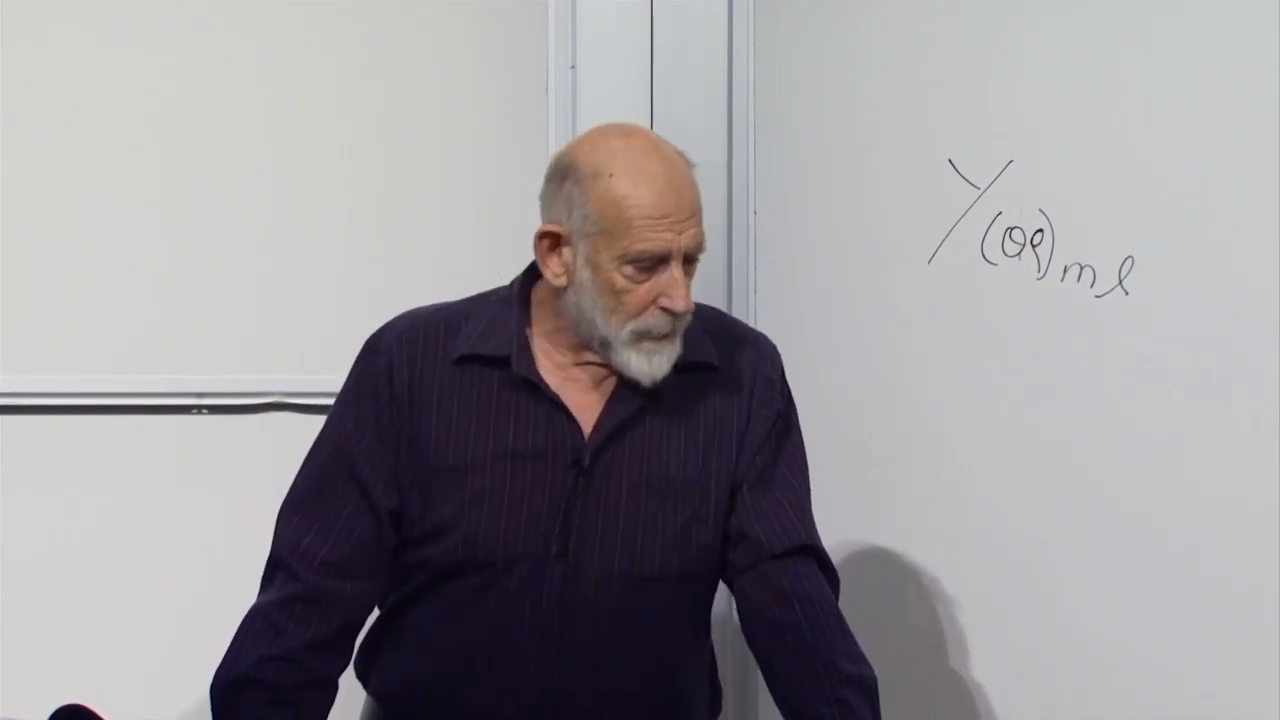
\includegraphics[width=0.9\linewidth]{lecture_03_frame_02.png}\caption{Bei festem klassischem Drehimpuls enthält der radiale Hamiltonoperator die radiale kinetische Energie, den Zentrifugalterm \(L^2/(2mr^2)\) und das Zentralpotential \(V(r)\).}\lectureframe{00:47:15}\end{figure}

Der Term \(1/r^2\) bildet die Zentrifugalbarriere. Sie steigt an, wenn sich das Teilchen dem Ursprung nähert, sodass die zugehörige Kraft nach außen gerichtet ist. Bei den hier betrachteten coulombartigen Anziehungspotentialen schwingt eine Bahn mit \(L\neq0\) um das Zentrum, statt es zu erreichen. Für \(L=0\) fehlt die Barriere.

Für das attraktive Coulombpotential gilt
\begin{equation}
V(r)=-\frac{\kappa}{r},
\end{equation}
Bei kleinen \(r\) dominiert der Zentrifugalterm, während der Coulombterm langsamer abfällt und bei großen \(r\) überwiegt. Für \(L\neq0\) besitzt die Summe ein Minimum. Die Bewegung am Minimum hat einen konstanten Radius und ist daher kreisförmig. Gebundene Bewegungen oberhalb des Minimums und unterhalb der Fluchtschwelle oszillieren zwischen einem minimalen und einem maximalen Radius; im Coulombproblem sind dies die radialen Oszillationen einer elliptischen Bahn.

\section{Die reduzierte Radialgleichung}

In der Quantenmechanik ist der Winkelanteil eines Zustands mit bestimmtem orbitalem Drehimpuls eine Kugelflächenfunktion. Wir schreiben den separierten Zustand als
\begin{equation}
\Psi_{n_r\ell m}(r,\theta,\phi)
=\frac{u_{n_r\ell}(r)}{r}\,
Y_{\ell m}(\theta,\phi).
\end{equation}
Der Winkeloperator \(L^2\) hat den Eigenwert
\begin{equation}
L^2Y_{\ell m}
=\hbar^2\ell(\ell+1)Y_{\ell m}.
\end{equation}
Für ein festes Wertepaar \(n_r,\ell\) kürzen wir \(u_{n_r\ell}(r)\) mit \(u(r)\) ab. Für die reduzierte Radialfunktion bleibt die Gleichung
\begin{equation}
\begin{aligned}
&-\frac{\hbar^2}{2m}\frac{d^2u}{dr^2}
+\frac{\hbar^2\ell(\ell+1)}{2mr^2}u(r)\\
&\qquad+V(r)u(r)=E_{n_r\ell}\,u(r).
\end{aligned}
\end{equation}

\editorialnote{Die rein eindimensionale Gleichung mit der zweiten Ableitung verwendet die reduzierte Radialfunktion \(u=rR\). Daher entspricht das \(\psi(r)\) in der dargestellten Vorlesungsgleichung \(u(r)\), während der gewöhnliche Radialfaktor in \(\Psi=R(r)Y_{\ell m}\) gleich \(R=u/r\) ist. Diese Konvention vermeidet, \(-i\hbar\,d/dr\) als eigenständigen hermiteschen Radialimpulsoperator im dreidimensionalen radialen Hilbertraum zu behandeln.}

Die reduzierte Radialgleichung ist unten an der Tafel zu sehen.\footnote{Ausgangsbild: \texttt{\detokenize{lecture_03_frame_03.png}}, Vorlesungsvideo bei \(00{:}54{:}32\).}

\begin{figure}[htbp]\centering
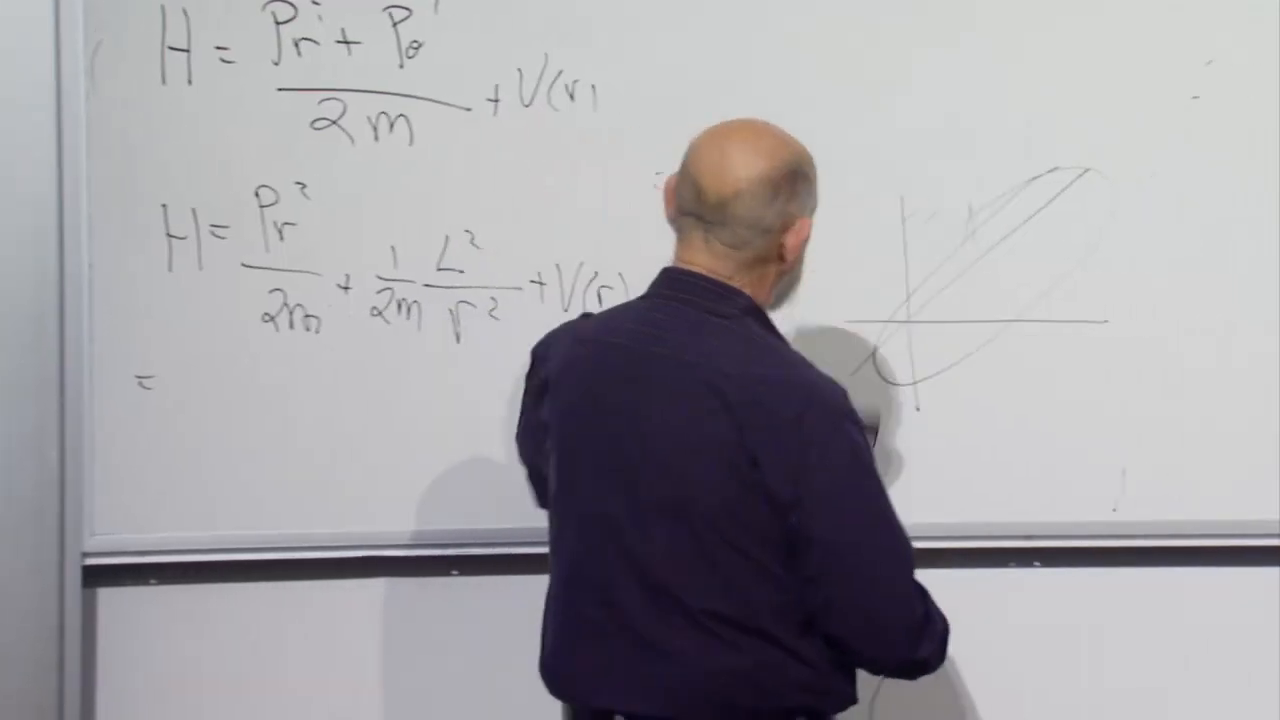
\includegraphics[width=0.9\linewidth]{lecture_03_frame_03.png}\caption{Bei festem \(\ell\) erfüllt die reduzierte Radialwellenfunktion eine eindimensionale Schr\"odinger-Gleichung mit einem Zentrifugalterm proportional zu \(\ell(\ell+1)/r^2\).}\lectureframe{00:54:32}\end{figure}

Die dreidimensionale Winkelstruktur ist im Parameter \(\ell\) zusammengefasst. Die magnetische Quantenzahl \(m\) tritt in der Radialgleichung nicht auf.

\begin{classroomqa}\lecturetimestamp{00:55:34}\audiencequestion{Haben die \(2\ell+1\) magnetischen Zustände bei gegebenem \(\ell\) dieselbe Energie?}\lecturerresponse{Ja, sofern auch der radiale Eigenzustand festgehalten wird. Bei jedem gewählten \(u_{n_r\ell}\) haben alle Werte \(m=-\ell,\ldots,\ell\) dieselbe Energie, weil \(m\) nicht in die Radialgleichung eingeht. Verschiedene radiale Eigenzustände bei demselben \(\ell\) haben im Allgemeinen unterschiedliche Energien.}\end{classroomqa}

\begin{classroomqa}\lecturetimestamp{00:56:03}\audiencequestion{Warum darf \(L^2\) durch \(\hbar^2\ell(\ell+1)\) ersetzt werden, und wie hängt \(\ell\) mit den erlaubten Werten von \(m\) zusammen?}\lecturerresponse{Die Zahl \(\ell\) kennzeichnet ein Drehimpulsmultiplett und ist der größte darin auftretende \(m\)-Wert. Alle Zustände dieses Multiplets haben denselben \(L^2\)-Eigenwert, nämlich \(\hbar^2\ell(\ell+1)\); dieser Eigenwert wird daher in die Radialgleichung eingesetzt.}\end{classroomqa}

Die expliziten Lösungen mit speziellen Funktionen werden für die vorliegende Argumentation nicht benötigt. Entscheidend ist, wie die Lösungen angeordnet sind.

\section{Radiale Knoten und Energieniveaus}

Bei festem \(\ell\) ist die reduzierte Radialgleichung ein gewöhnliches eindimensionales Eigenwertproblem. Seine gebundenen Zustände sind nach der Zahl ihrer inneren Knoten geordnet. Der niedrigste radiale Zustand hat keinen inneren Knoten, der nächste einen und der darauffolgende zwei. Eine größere Knotenzahl bedeutet, dass sich die Wellenfunktion schneller ändert; dadurch ist der Impuls größer und folglich auch die kinetische Energie.

Jeder Wert von \(\ell\) definiert einen anderen radialen Operator, denn der Zentrifugalterm ändert sich mit \(\ell\). Somit bilden \(\ell=0,1,2,\ldots\) getrennte radiale Niveautürme. Der positive Zentrifugalterm verschiebt die Niveaus nach oben, wenn der Drehimpuls zunimmt. Jeder radiale Eigenwert bei festem \(\ell\) gehört zu einem magnetischen Multiplett der Dimension
\begin{equation}
2\ell+1.
\end{equation}
Die Niveaus mit \(\ell=0\) sind Singuletts, diejenigen mit \(\ell=1\) Tripletts und diejenigen mit \(\ell=2\) Quintetts. Dies sind die durch die Rotationssymmetrie gewährleisteten Entartungen; eine zusätzliche Symmetrie kann auch Zustände mit verschiedenen Werten von \(\ell\) entarten lassen.

Für Potentiale vom Typ eines Atompotentials, die die Bedingung \(V(r)\to0\) bei großen \(r\) erfüllen, liegt die Fluchtschwelle üblicherweise bei \(E=0\). Die Zustände mit negativer Energie bilden das diskrete gebundene Spektrum. Bei und oberhalb von \(E=0\) liegt das Streukontinuum vor. Diese Aussage hängt vom Verhalten des Potentials bei großen \(r\) ab und gilt nicht für ein einschließendes Zentralpotential.

\section{Die besondere Coulomb-Entartung}

Beim exakten nichtrelativistischen Coulombpotential fallen zusätzlich bestimmte Energieniveaus zusammen. Der niedrigste radiale Zustand mit \(\ell=1\) hat dieselbe Energie wie der erste angeregte Zustand mit \(\ell=0\). Der nächsthöhere Zustand mit \(\ell=1\) fällt mit dem zweiten angeregten Zustand mit \(\ell=0\) zusammen; auch der niedrigste Zustand mit \(\ell=2\) gehört zu dieser Gruppe. Das Muster setzt sich bei den höheren radialen und Drehimpulstürmen fort.

\begin{classroomqa}\lecturetimestamp{01:09:57}\audiencequestion{Deutet diese zusätzliche Coulomb-Entartung auf eine weitere Symmetrie hin?}\lecturerresponse{Ja. Sie beruht auf einer ungewöhnlichen zusätzlichen Symmetrie des exakten Coulombpotentials. Kleine Änderungen des Potentials heben das Zusammenfallen der Niveaus auf; die Herleitung wird hier nicht behandelt.}\end{classroomqa}

Die daraus resultierenden Entartungsgrade der orbitalen Schalen sind
\begin{equation}
1,\qquad 4,\qquad 9,\qquad 16,\qquad \ldots
\end{equation}
noch ohne Berücksichtigung des Elektronenspins.

\begin{classroomqa}\lecturetimestamp{01:11:46}\audiencequestion{Gilt diese Entartung für Wasserstoff oder nur für das ideale Coulombproblem?}\lecturerresponse{Für Wasserstoff gilt sie mit sehr guter Näherung, aber nicht exakt. Relativistische Korrekturen und die endliche Größe des Atomkerns stören das ideale Coulombmuster.}\end{classroomqa}

Ein punktförmiger Kern erzeugt ein exaktes \(1/r\)-Potential. Ist die Kernladung über ein kleines Volumen verteilt, entsteht ein leicht anderes Potential, wenn das Elektron in dieses Volumen eindringt. Selbst diese kleine Abweichung hebt einen Teil der besonderen Entartung auf.

Auch der Spin wurde bisher nicht berücksichtigt. Bezieht man die beiden Elektronenspinzustände ein, verdoppeln sich die Schalenbesetzungszahlen zu
\begin{equation}
2,\qquad 8,\qquad 18,\qquad 32,\qquad \ldots
\end{equation}
bevor die weiteren Aufspaltungen einer vollständigeren atomaren Beschreibung berücksichtigt werden.

\section{Noch einmal zur kartesischen Gleichung}

Die Gleichung, von der das Radialproblem ausging, ist die dreidimensionale zeitunabhängige Schr\"odinger-Gleichung
\begin{equation}
\begin{aligned}
-\frac{\hbar^2}{2m}\nabla^2\Psi+V(r)\Psi&=E\Psi,\\
\nabla^2&=\frac{\partial^2}{\partial x^2}
+\frac{\partial^2}{\partial y^2}
+\frac{\partial^2}{\partial z^2},\\
r&=\sqrt{x^2+y^2+z^2}.
\end{aligned}
\end{equation}
Wir wechseln zu Radial- und Winkelkoordinaten und wählen einen Eigenzustand von \(L^2\).
Ersetzt man \(L^2\) durch \(\hbar^2\ell(\ell+1)\), so wird die partielle Differentialgleichung auf die oben angegebene gewöhnliche Radialgleichung reduziert.

\begin{classroomqa}\lecturetimestamp{01:16:42}\audiencequestion{Lässt sich aus Abweichungen vom idealen Coulombspektrum die Größe des Atomkerns bestimmen?}\lecturerresponse{Nicht durch diesen einfachen Vergleich. Andere Korrekturen sind viel größer und müssen zuerst berücksichtigt werden. Die Kerngröße wird hier erwähnt, weil sie unmittelbar ein Beispiel für eine Abweichung vom Punkt-Coulombpotential liefert.}\end{classroomqa}

\begin{classroomqa}\lecturetimestamp{01:17:09}\audiencequestion{Was ist der wichtigste Unterschied zwischen den klassischen und quantenmechanischen Drehimpulstermen?}\lecturerresponse{Klassisch ist \(L^2\) einfach das Quadrat des Betrags eines erhaltenen Vektors. In einem quantenmechanischen orbitalen Multiplett ist der Eigenwert \(\hbar^2\ell(\ell+1)\) und nicht einfach \(\hbar^2\ell^2\). Der zusätzliche Term ergibt sich aus der Nichtvertauschbarkeit der Drehimpulskomponenten.}\end{classroomqa}

\begin{classroomqa}\lecturetimestamp{01:17:58}\audiencequestion{Haben die Wellenfunktionen gebundener Zustände kompakten Träger?}\lecturerresponse{Nein. Sie erstrecken sich beliebig weit vom Zentrum weg. Bei den hier betrachteten gebundenen Atomzuständen fallen sie bei großen Abständen exponentiell ab. Die Wahrscheinlichkeit wird dadurch vernachlässigbar klein, verschwindet aber nicht außerhalb irgendeines endlichen Radius.}\end{classroomqa}

\begin{classroomqa}\lecturetimestamp{01:18:48}\audiencequestion{Was geschieht mit dem stabilen Punkt, wenn \(\ell=0\) die Zentrifugalmulde beseitigt?}\lecturerresponse{Ein Minimum, das aus dem Zusammenspiel von Zentrifugalbarriere und Anziehung entsteht, gibt es dann nicht mehr. Im idealisierten Punkt-Coulombpotential bewegt sich das klassische Teilchen auf das singuläre Zentrum zu. Quantenmechanisch kann der niedrigste Zustand nicht zugleich eine exakt bestimmte Position im Zentrum und einen Impuls von null haben; daher weist die Wellenfunktion des niedrigsten Zustands eine endliche räumliche Ausdehnung auf.}\end{classroomqa}

\editorialnote{Bei einem regulären Zentralpotential kann eine klassische Bahn mit Drehimpuls null durch den Ursprung weiterlaufen. Beim idealen Punkt-Coulombpotential ist \(r=0\) dagegen eine Kollisionssingularität; die Fortsetzung der klassischen Bahn erfordert eine zusätzliche Vorschrift.}

Bei der klassischen Reduktion wurde eine einzelne Bahn in eine Ebene gelegt. Dieser Schritt lässt sich jedoch nicht auf dieselbe Weise auf eine quantenmechanische Wellenfunktion anwenden. Ein orbitaler Quantenzustand erstreckt sich über den dreidimensionalen Raum. Der vollständige Winkeloperator lautet \(L^2=L_x^2+L_y^2+L_z^2\), und sein Eigenwert bewahrt das dreidimensionale Ergebnis \(\hbar^2\ell(\ell+1)\).

\begin{classroomqa}\lecturetimestamp{01:21:30}\audiencequestion{Wie kann das quantenmechanische Problem dreidimensional bleiben, nachdem die klassische Bahn in eine Ebene gelegt wurde?}\lecturerresponse{Nur die klassische Bahn wurde durch eine Koordinatenwahl in eine feste Ebene gelegt, deren Normale parallel zum erhaltenen Drehimpulsvektor ist. Eine quantenmechanische Wellenfunktion nimmt den dreidimensionalen Raum ein. Die übrigen Drehimpulskomponenten bleiben über \(L^2\) erhalten. Deshalb enthält die Radialgleichung \(\ell(\ell+1)\) und nicht nur das Quadrat einer einzelnen Komponente.}\end{classroomqa}

\begin{classroomqa}\lecturetimestamp{01:22:54}\audiencequestion{Gibt es in jedem quantenmechanischen Problem Erzeugungs- und Vernichtungsoperatoren?}\lecturerresponse{Nein. Sie treten in besonders günstigen Fällen auf. Der Drehimpuls ist ein solcher Fall, der harmonische Oszillator ein weiterer. Der Oszillator ist besonders nützlich, weil die Bewegung in der Nähe eines stabilen Gleichgewichts so häufig näherungsweise harmonisch ist. Dazu gehören kleine radiale Schwingungen nahe dem Minimum eines effektiven Potentials.}\end{classroomqa}

An dieser Stelle wird das Atomproblem zurückgestellt. Als nächstes Beispiel folgt der harmonische Oszillator, dessen Spektrum sich mithilfe von Leiteroperatoren bestimmen lässt.

\section{Kleine Schwingungen und der harmonische Oszillator}

In der Nähe eines stabilen Gleichgewichts führt eine hinreichend kleine Auslenkung häufig zu harmonischer Bewegung. Das effektive Radialpotential bei von null verschiedenem Drehimpuls liefert ein Beispiel dafür: Nahe dem Tiefpunkt seiner Mulde ist die radiale Bewegung näherungsweise harmonisch.

Betrachten wir einen eindimensionalen Oszillator mit Einheitsmasse. Die Auslenkung aus der Gleichgewichtslage sei \(x\), und die Federkonstante schreiben wir als \(k=\omega^2\). Der klassische Hamiltonian lautet
\begin{equation}
H=\frac{p^2}{2}+\frac{\omega^2x^2}{2}.
\end{equation}
Aus den Hamilton-Gleichungen folgt
\begin{equation}
\dot{x}=\frac{\partial H}{\partial p}=p,
\qquad
\dot{p}=-\frac{\partial H}{\partial x}=-\omega^2x,
\end{equation}
und damit
\begin{equation}
\ddot{x}=-\omega^2x.
\end{equation}
Somit ist \(\omega\) die klassische Schwingungsfrequenz.

\section{Faktorisierung und Nullpunktsenergie}

Quantenmechanisch gilt
\begin{equation}
[x,p]=i\hbar.
\end{equation}
Der Hamiltonoperator ist eine Summe von Quadraten, was eine Faktorisierung nahelegt:
\begin{align}
\frac{1}{2}(p+i\omega x)(p-i\omega x)
&=\frac{1}{2}\left(p^2+\omega^2x^2+i\omega[x,p]\right) \\
&=\frac{1}{2}\left(p^2+\omega^2x^2-\hbar\omega\right).
\end{align}
Daraus folgt
\begin{equation}
H=\frac{1}{2}(p+i\omega x)(p-i\omega x)
+\frac{1}{2}\hbar\omega.
\end{equation}
Der additive Term \(\hbar\omega/2\) ist die Nullpunktsenergie.

Klassisch würde die niedrigste Energie bei \(x=p=0\) auftreten. Quantenmechanisch kann kein Zustand sowohl einen exakt festgelegten Ort als auch einen exakt festgelegten Impuls gleich null haben. Zudem sind die beiden Terme \(p^2/2\) und \(\omega^2x^2/2\) positiv und können einander nicht aufheben. Eine von null verschiedene Grundzustandsenergie ist daher unvermeidlich.

Für die Berechnung mit den Leiteroperatoren kann die gemeinsame additive Konstante vorübergehend beiseitegelassen und am Ende wieder hinzugefügt werden.

\begin{classroomqa}\lecturetimestamp{01:36:10}\audiencequestion{Lässt sich aus dem positiven Vorzeichen des Nullpunktsenergie-Terms noch etwas Weiteres schließen?}\lecturerresponse{Der Hamiltonoperator des Oszillators ist positiv: Er ist eine Summe positiver Quadrate, daher kann seine Energie nicht negativ sein.}\end{classroomqa}

\section{Die Leiter des Oszillators}

Wir führen die dimensionslosen Operatoren ein.\footnote{In \(01{:}37\)--\(01{:}42\) wird mit \(\hbar=1\) gerechnet. In diesen normierten Definitionen wird der Faktor \(\hbar\) wieder eingesetzt, sodass \(A_\pm\) dimensionslos sind und ihr Kommutator eins beträgt.}
\begin{equation}
A_+=\frac{p+i\omega x}{\sqrt{2\hbar\omega}},
\qquad
A_-=\frac{p-i\omega x}{\sqrt{2\hbar\omega}}.
\end{equation}
Sie sind zueinander adjungiert:
\begin{equation}
A_+^\dagger=A_-.
\end{equation}
Ihr Kommutator lautet
\begin{align}
[A_-,A_+]
&=\frac{1}{2\hbar\omega}
\left([p,i\omega x]+[-i\omega x,p]\right) \\
&=1.
\end{align}

Wir definieren
\begin{equation}
N=A_+A_-.
\end{equation}
Dann lautet der Hamiltonoperator
\begin{equation}
H=\hbar\omega\left(N+\frac{1}{2}\right).
\end{equation}
Damit reduziert sich die Bestimmung des Energiespektrums auf die Bestimmung der Eigenwerte von \(N\).

Es sei
\begin{equation}
N|n\rangle=n|n\rangle.
\end{equation}
Die Kommutatoren mit \(N\) lauten wie folgt.\footnote{Die Zwischenschritte bei \(01{:}45{:}37\)--\(01{:}48{:}10\) lassen sich unmittelbar aus den angegebenen Relationen \(N=A_+A_-\) und \([A_-,A_+]=1\) rekonstruieren.}
\begin{align}
[N,A_+]
&=A_+[A_-,A_+]=A_+, \\
[N,A_-]
&=[A_+,A_-]A_-=-A_-.
\end{align}
Daraus folgt
\begin{align}
N\bigl(A_+|n\rangle\bigr)
&=(n+1)A_+|n\rangle, \\
N\bigl(A_-|n\rangle\bigr)
&=(n-1)A_-|n\rangle.
\end{align}
Somit erhöht \(A_+\) einen Eigenwert von \(N\) um eins und \(A_-\) verringert ihn um eins, sofern der resultierende Vektor nicht verschwindet.

Der Operator \(N\) ist nichtnegativ:
\begin{equation}
\langle\psi|N|\psi\rangle
=\langle\psi|A_+A_-|\psi\rangle
=\|A_-|\psi\rangle\|^2
\geq0.
\end{equation}
Der Absenkprozess kann daher nicht zu negativen Eigenwerten führen. Bei einem untersten Zustand \(|b\rangle\) muss er enden:
\begin{equation}
A_-|b\rangle=0.
\end{equation}

Bei normierten Eigenzuständen sind die Koeffizienten der Leiter durch ihre Normen festgelegt:
\begin{align}
\|A_-|n\rangle\|^2
&=\langle n|A_+A_-|n\rangle=n, \\
\|A_+|n\rangle\|^2
&=\langle n|A_-A_+|n\rangle=n+1.
\end{align}
Die Phasen lassen sich daher so wählen, dass
\begin{equation}
A_-|n\rangle=\sqrt{n}\,|n-1\rangle,
\qquad
A_+|n\rangle=\sqrt{n+1}\,|n+1\rangle.
\end{equation}

\begin{classroomqa}\lecturetimestamp{01:52:42}\audiencequestion{Wenn \(A_-\) einen Zustand absenkt und \(A_+\) ihn wieder anhebt, wie ergibt \(A_+A_-\) dann den Eigenwert \(n\)?}\lecturerresponse{Die Wirkung der Leiter enthält Normierungsfaktoren. Die Anwendung von \(A_-\) liefert den Faktor \(\sqrt n\), und bei der anschließenden Anwendung von \(A_+\) auf den resultierenden Zustand kommt ein weiterer Faktor \(\sqrt n\) hinzu. Ihr Produkt ist \(n\).}\end{classroomqa}

Tatsächlich gilt
\begin{equation}
A_+A_-|n\rangle
=\sqrt n\,A_+|n-1\rangle
=n|n\rangle.
\end{equation}

\begin{classroomqa}\lecturetimestamp{01:55:52}\audiencequestion{Muss der niedrigste Eigenwert von \(N\) null sein, oder könnte er positiv sein?}\lecturerresponse{Er muss null sein, und das Spektrum von \(N\) besteht aus den nichtnegativen ganzen Zahlen. Der Beweis für diesen Endpunkt wurde noch nicht erbracht.}\end{classroomqa}

\editorialnote{Sei \(|b\rangle\) ein Zustand mit dem niedrigsten Eigenwert. Da der Absenkprozess enden muss, gilt \(A_-|b\rangle=0\). Daraus folgt unmittelbar \(N|b\rangle=A_+A_-|b\rangle=0\); der niedrigste Eigenwert von \(N\) ist also null.}

Ausgehend von diesem untersten Zustand erhalten wir durch wiederholte Anwendung von \(A_+\)
\begin{equation}
n=0,1,2,\ldots.
\end{equation}
Nach Wiederherstellung des additiven Nullpunktsenergie-Terms lauten die Oszillatorenergien
\begin{equation}
E_n=\hbar\omega\left(n+\frac{1}{2}\right),
\qquad n=0,1,2,\ldots.
\end{equation}

Die Oszillatoralgebra wird weiterentwickelt und zur Lösung anderer quantenmechanischer Probleme eingesetzt.
\chapter{Oszillator-Wellenfunktionen, Spin-einhalb und Teilchenaustausch}

\section{Oszillatoren überall}

Jedes System mit einem stabilen Gleichgewicht kann schwingen, wenn es aus diesem Gleichgewicht ausgelenkt wird. Es kann eine oder mehrere Frequenzen haben. Eine Violinsaite besitzt zum Beispiel eine Grundschwingung und höhere Harmonische. Zupft man sie an, wird eine bestimmte Kombination dieser Schwingungsmoden angeregt.

Die wichtigeren Beispiele hier sind Felder. Die Gleichgewichtskonfiguration des elektromagnetischen Feldes ist das Vakuum: kein elektrisches Feld, kein magnetisches Feld und keine elektromagnetische Schwingung. Strahlt man in einen Hohlraum oder einen Wellenleiter ein, kann das Feld in seinen erlaubten Moden schwingen, jede mit ihrer eigenen Frequenz. In der Quantentheorie beschreiben diese Moden Ansammlungen von Photonen.

Dieselbe Idee gilt für einen Kristall. Es wäre irreführend, sich jedes Atom als unabhängigen Oszillator vorzustellen. Die Atome üben Kräfte aufeinander aus, sodass die Auslenkung eines Atoms seine Nachbarn beeinflusst und eine Welle durch den Kristall läuft. Die Normalmoden dieser gekoppelten Bewegung sind harmonische Oszillatoren; ihre Quanten heißen Phononen. Photonen und Phononen sind unterschiedliche physikalische Objekte, führen aber beide zurück zur selben Oszillatoralgebra.

\section{Die Oszillatoralgebra}

Für die Betrachtung des Oszillators setzen wir Masse und reduziertes Plancksches Wirkungsquantum gleich eins:
\[
m=1,\qquad \hbar=1.
\]
Der Hamiltonoperator lautet
\begin{equation}
H=\frac{p^{2}}{2}+\frac{\omega^{2}x^{2}}{2}.
\end{equation}
Der Parameter \(\omega\) legt die Krümmung des Potentials fest und ist zugleich die Schwingungsfrequenz.

Wir definieren die Auf- und Absteigeoperatoren durch
\begin{equation}
A_{\pm}=\frac{p\pm i\omega x}{\sqrt{2\omega}}.
\end{equation}
Die Normierung ist so gewählt, dass
\begin{equation}
[A_{-},A_{+}]=1.
\end{equation}
Der Zahloperator ist
\begin{equation}
N=A_{+}A_{-}.
\end{equation}
Zusammen bedeuten diese Gleichungen, dass \(A_{+}\) einen Eigenwert von \(N\) um eins erhöht und \(A_{-}\) ihn um eins erniedrigt. Das resultierende Spektrum lautet
\begin{equation}
n=0,1,2,3,\ldots .
\end{equation}

Das Produkt der beiden Leiteroperatoren macht auch die quantenmechanische Korrektur der klassischen Energie sichtbar:
\begin{align}
N
&=\frac{1}{2\omega}(p+i\omega x)(p-i\omega x)\\
&=\frac{1}{2\omega}\left(p^{2}+\omega^{2}x^{2}
 +i\omega[x,p]\right)\\
&=\frac{1}{2\omega}\left(p^{2}+\omega^{2}x^{2}-\omega\right),
\end{align}
wobei \([x,p]=i\) gilt. Folglich ist
\begin{equation}
H=\omega\left(N+\frac12\right).
\end{equation}
Ist die additive Konstante für das Problem unerheblich, verwendet man zweckmäßig den verschobenen Hamiltonoperator
\begin{equation}
H_{\mathrm{shifted}}=H-\frac{\omega}{2}=\omega N.
\end{equation}
Der Term \(\omega/2\) ist die Nullpunktsenergie oder Grundzustandsenergie des Oszillators. Bei einer Feldmode heißt der entsprechende Term Vakuumenergie. Er spiegelt die Unschärferelation wider: Kein Zustand kann zugleich \(x\) und \(p\) exakt gleich null haben; daher können die beiden positiven quadratischen Terme in \(H\) nicht beide den Erwartungswert null haben.

\begin{classroomqa}
\lecturetimestamp{00:09:46}
\audiencequestion{Warum gehört null zum Spektrum des Zahloperators?}
\lecturerresponse{Das lässt sich explizit zeigen, indem man die Wellenfunktion des Grundzustands konstruiert. Dabei wird ein Zustand mit \(N=0\) sichtbar.}
\end{classroomqa}

Beginnen wir diese Konstruktion, indem wir Zustandsvektoren durch Ortswellenfunktionen ersetzen. Die Energieeigenzustände werden zu
\[
\psi_{0}(x),\ \psi_{1}(x),\ \psi_{2}(x),\ldots,
\]
und die Grundoperatoren wirken als
\begin{equation}
X\longmapsto x,\qquad
P\longmapsto -i\frac{d}{dx}.
\end{equation}
Stellt man \(\hbar\) wieder her, lautet die zweite Ersetzung
\(P\mapsto-i\hbar\,d/dx\).

Bevor wir \(\psi_{0}\) bestimmen, gibt es eine schnellere, abstrakte Antwort auf die Frage. Auf der diskreten Leiter der normierbaren Oszillatoreigenzustände ist \(N=A_{+}A_{-}\) nichtnegativ; wiederholtes Absteigen in Einerschritten kann daher nicht unbegrenzt weitergehen. Am Endpunkt---dessen normierbare Wellenfunktion wir unten konstruieren---muss es einen Zustand geben, bezeichnet mit \(\lvert0\rangle\), für den gilt:
\begin{equation}
A_{-}\lvert0\rangle=\mathbf 0.
\end{equation}
Andernfalls wäre \(A_{-}\lvert0\rangle\) ein weiterer Zustand eine Stufe tiefer. Daraus folgt unmittelbar
\begin{equation}
N\lvert0\rangle
=A_{+}A_{-}\lvert0\rangle
=\mathbf 0
=0\,\lvert0\rangle.
\end{equation}
Der unterste Zustand hat also den Zahleneigenwert null.

\begin{classroomqa}
\lecturetimestamp{00:14:57}
\audiencequestion{Wenn null der Eigenwert ist, müsste dann auf der rechten Seite ein Eigenvektor zum Eigenwert null stehen?}
\lecturerresponse{Das Ket \(\lvert0\rangle\) ist ein normierter, von null verschiedener Vektor mit der Bezeichnung null. In \(N\lvert0\rangle=0\,\lvert0\rangle\) ist die rechte Seite der Nullvektor. Das Ket des Grundzustands und der Nullvektor sind verschiedene Objekte.}
\end{classroomqa}

\section{Die Schr\"odinger-Gleichung und physikalische Lösungen}

Kehren wir nun zur Ortsdarstellung zurück. Die zeitunabhängige Schr\"odinger-Gleichung lautet
\begin{equation}
\left[
-\frac12\frac{d^{2}}{dx^{2}}
+\frac12\omega^{2}x^{2}
\right]\psi(x)=E\psi(x).
\end{equation}
Als Differentialgleichung zweiter Ordnung besitzt sie formale Lösungen für beliebige Werte von \(E\). Die meisten dieser formalen Lösungen sind keine physikalischen Osillatorzustände. Für große \(\lvert x\rvert\) wachsen sie exponentiell, sodass ihre Norm divergiert.

Für einen gebundenen Zustand muss die Wellenfunktion quadratintegrabel sein:
\begin{equation}
\int_{-\infty}^{\infty}\psi^{*}(x)\psi(x)\,dx<\infty.
\end{equation}
Dann kann sie so normiert werden, dass das Integral eins ergibt. Nur bestimmte Energiewerte liefern solche Lösungen. Orts- und Impulszustände auf einer unendlichen Geraden sind diesbezüglich Ausnahmefälle; exponentiell anwachsende Oszillatorlösungen werden dagegen einfach aus dem Zustandsraum ausgeschlossen.

\section{Der gaußförmige Grundzustand}

Die Differentialgleichung zweiter Ordnung lässt sich lösen, doch die Leiteralgebra liefert eine einfachere Gleichung erster Ordnung:
\begin{equation}
A_{-}\psi_{0}(x)=0.
\end{equation}
Der Vorfaktor in \(A_{-}\) ist unerheblich, wenn die rechte Seite null ist; dies ist daher äquivalent zu
\begin{equation}
(p-i\omega x)\psi_{0}(x)=0.
\end{equation}
Mit \(p=-i\,d/dx\) ergibt sich
\begin{equation}
\left(\frac{d}{dx}+\omega x\right)\psi_{0}(x)=0.
\end{equation}

\begin{classroomqa}
\lecturetimestamp{00:22:32}
\audiencequestion{Lässt sich das durch Trennung der Variablen lösen?}
\lecturerresponse{Es gibt nur eine unabhängige Variable, also keine zwei Variablen, die man trennen könnte. In der Form \(\psi_{0}'/\psi_{0}=-\omega x\) hat die Gleichung die Gestalt einer logarithmischen Ableitung. Das legt nahe, die Wellenfunktion als Exponentialfunktion anzusetzen.}
\end{classroomqa}

Eine nützliche Lösungsmethode besteht darin, anzusetzen:
\begin{equation}
\psi_{0}(x)=e^{f(x)}.
\end{equation}
Dann gilt
\[
\psi_{0}'(x)=f'(x)e^{f(x)},
\]
und der gemeinsame Exponentialfaktor kürzt sich heraus. Die Gleichung vereinfacht sich zu
\begin{equation}
\frac{df}{dx}+\omega x=0.
\end{equation}

\begin{classroomqa}
\lecturetimestamp{00:26:28}
\audiencequestion{Müsste in \(f(x)\) ein Minuszeichen stehen?}
\lecturerresponse{Ja. Da \(df/dx=-\omega x\) gilt, ergibt die Integration einen negativen quadratischen Term.}
\end{classroomqa}

Somit gilt
\begin{equation}
f(x)=-\frac12\omega x^{2}+C,
\end{equation}
und
\begin{equation}
\psi_{0}(x)\propto e^{-\omega x^{2}/2}.
\end{equation}
Die multiplikative Normierungskonstante bleibt unbestimmt. Entscheidend ist die gaußförmige Gestalt: Die Wellenfunktion ist glatt, um den Ursprung konzentriert und fällt für große \(\lvert x\rvert\) rasch ab. Sie ist offensichtlich quadratintegrabel.

Man muss die Lösung nicht in die Differentialgleichung zweiter Ordnung einsetzen, um ihre Energie zu bestimmen. Die Algebra liefert bereits
\begin{equation}
E_{0}=\frac{\omega}{2}.
\end{equation}

\section{Angeregte Zustände, Knoten und klassische Bewegung}

Der erste angeregte Zustand ergibt sich, indem man auf den Grundzustand den Aufsteigeoperator anwendet:
\begin{equation}
\psi_{1}(x)\propto A_{+}\psi_{0}(x)
\propto(p+i\omega x)e^{-\omega x^{2}/2}.
\end{equation}
Die Grundzustandsgleichung besagt
\[
p\psi_{0}=i\omega x\,\psi_{0}.
\]
Durch das Vorzeichenwechseln im Leiteroperator wird aus der Auslöschung eine Addition:
\begin{equation}
(p+i\omega x)\psi_{0}
=2i\omega x\,\psi_{0}.
\end{equation}
Bis auf einen Gesamtfaktor gilt
\begin{equation}
\psi_{1}(x)\propto x\,e^{-\omega x^{2}/2}.
\end{equation}

Diese Wellenfunktion ist ungerade:
\begin{equation}
\psi_{1}(-x)=-\psi_{1}(x).
\end{equation}
Ihre Wahrscheinlichkeitsdichte ist gerade, hat aber am Ursprung einen Knoten:
\begin{equation}
\lvert\psi_{1}(0)\rvert^{2}=0.
\end{equation}
Die Wahrscheinlichkeitsdichte des ersten angeregten Zustands hat also bei \(x=0\) einen Knoten.

Wiederholte Anwendung von \(A_{+}\) liefert Polynome höheren Grades, die mit derselben gaußförmigen Einhüllenden multipliziert sind.\footnote{Die Vorlesung nennt die Polynomfaktoren höheren Grades, den bei jedem Schritt hinzukommenden Knoten und den Symmetriewechsel von \(00{:}34{:}25\) bis \(00{:}35{:}49\). Die Form als Produkt aus Gaußfunktion und Polynom wird durch Leonard Susskind und Art Friedman, \emph{Quantum Mechanics: The Theoretical Minimum} (2014), in ihrer Behandlung der Oszillatoreigenfunktionen bestätigt.} Bis auf einen Normierungsfaktor gilt
\begin{equation}
\psi_{n}(x)=P_{n}(x)e^{-\omega x^{2}/2}.
\end{equation}
Die Parität wechselt zwischen gerade und ungerade, und bei jedem Schritt kommt ein Knoten hinzu. Mit wachsendem \(n\) breitet sich die Wellenfunktion weiter vom Ursprung aus und weist raschere Oszillationen auf.

Diese beiden Eigenschaften haben direkte physikalische Bedeutungen. Eine größere Ausdehnung vom Ursprung entspricht einer höheren potenziellen Energie, weil das Potential wie \(x^{2}\) anwächst. Rasche Oszillationen im Ortsraum signalisieren einen größeren Impuls. Ein stark angeregter Oszillator gelangt wahrscheinlich weiter vom Zentrum weg; beim Durchgang durch den Zentralbereich trägt er mehr Impuls, und seine Wellenfunktion oszilliert dort rascher.

\begin{classroomqa}
\lecturetimestamp{00:37:18}
\audiencequestion{Nähert sich der harmonische Oszillator keinem klassischen Verhalten an, wenn \(n\) groß wird?}
\lecturerresponse{Klassische Bewegung wird nicht durch einen einzigen stationären Energieeigenzustand beschrieben. Sie zeigt sich in einem Wellenpaket, das viele Energieniveaus enthält. Eine verschobene Gaußfunktion entwickelt sich beispielsweise wie ein klassischer Oszillator hin und her, und die relative Unschärfe wird kleiner, je größer die Schwingungsamplitude ist.}
\end{classroomqa}

Beginnen wir mit der gaußförmigen Wellenfunktion des Grundzustands und verschieben sie vom Ursprung weg. Das verschobene Wellenpaket ist kein Energieeigenzustand mehr, sondern eine Überlagerung vieler solcher Zustände. Unter der zeitabhängigen Schr\"odinger-Gleichung sammeln seine Komponenten unterschiedliche Phasen an. Das Paket schwingt von einer Seite des Potentials zur anderen, wobei es nahe dem Zentrum eine rasche Phasenvariation entwickelt und an einem Umkehrpunkt wieder glatt wird. Je größer die Auslenkung im Verhältnis zur Breite des Pakets ist, desto klassischer erscheint die Bewegung.

\begin{classroomqa}
\lecturetimestamp{00:39:29}
\audiencequestion{Müsste die Wellenfunktion des zweiten angeregten Zustands am Ursprung null sein?}
\lecturerresponse{Nein. Ihr Polynomfaktor ist nicht einfach \(x^{2}\); er enthält auch einen konstanten Term, sodass die Wellenfunktion bei \(x=0\) nicht notwendigerweise verschwindet.}
\end{classroomqa}

Das Leiterargument setzt außerdem voraus, dass \(A_{+}\) und \(A_{-}\) auf dem quadratintegrablen Oszillatordomänenbereich hermitesch konjugiert sind und das für die Adjungiertheitsrelation erforderliche Randverhalten erfüllen. Exponentiell anwachsende formale Lösungen gehören nicht zu diesem Definitionsbereich.

\begin{classroomqa}
\lecturetimestamp{00:40:45}
\audiencequestion{Gibt es eine allgemeine Methode zu erkennen, ob sich ein Hamiltonoperator mit diesen algebraischen Methoden lösen lässt?}
\lecturerresponse{Eine solche allgemeine Regel gibt es nicht. Exakt lösbare Beispiele sind selten. Der harmonische Oszillator und das ideale nichtrelativistische Wasserstoffatom sind glückliche Fälle, in denen algebraische Methoden funktionieren.}
\end{classroomqa}

\section{Spin-einhalb als Drehimpuls}

Spin ist ein Drehimpuls, den ein Teilchen unabhängig von seiner Schwerpunktsbahbewegung trägt. Ein ruhendes Teilchen besitzt keinen Bahndrehimpuls \(\mathbf R\times\mathbf P\), kann aber dennoch Spin haben. Man kann versuchen, sich ein winziges rotierendes Objekt vorzustellen, oder Spin als intrinsische Quanteneigenschaft auffassen. Entscheidend ist die mathematische Aussage: Seine Komponenten transformieren sich unter räumlichen Drehungen und erfüllen die Kommutationsrelationen des Drehimpulses.

Von hier an stellen wir \(\hbar\) wieder her. Die Drehimpulskomponenten erfüllen
\begin{equation}
[L_{z},L_{x}]=i\hbar L_{y},
\end{equation}
wobei sich die beiden anderen Relationen durch zyklische Vertauschung ergeben. Die dimensionslosen Pauli-Matrizen sind
\begin{equation}
\begin{aligned}
\sigma_{z}&=
\begin{pmatrix}
1&0\\
0&-1
\end{pmatrix},\\[0.4em]
\sigma_{x}&=
\begin{pmatrix}
0&1\\
1&0
\end{pmatrix},\\[0.4em]
\sigma_{y}&=
\begin{pmatrix}
0&-i\\
i&0
\end{pmatrix}.
\end{aligned}
\end{equation}
In dieser Basis ist \(\sigma_{z}\) diagonal. Seine Eigenwerte sind \(+1\) und
\(-1\).

\begin{classroomqa}
\lecturetimestamp{00:47:35}
\audiencequestion{Müsste in \(\sigma_x\) ein Minuszeichen stehen?}
\lecturerresponse{Nein. Beide Nebendiagonalelemente von \(\sigma_x\) sind positiv.}
\end{classroomqa}

Die Tafelrechnung bei \(00{:}49{:}35\) beginnt mit der Multiplikation der einzelnen Matrixeinträge. Führt man die Produkte vollständig aus, erhält man
\begin{align}
\sigma_{z}\sigma_{x}
&=
\begin{pmatrix}
0&1\\
-1&0
\end{pmatrix}
=i\sigma_{y},\\
\sigma_{x}\sigma_{z}
&=
\begin{pmatrix}
0&-1\\
1&0
\end{pmatrix}
=-i\sigma_{y}.
\end{align}
Damit gilt
\begin{equation}
[\sigma_{z},\sigma_{x}]=2i\sigma_{y}.
\end{equation}
Der zusätzliche Faktor zwei entfällt, wenn man die physikalischen Spinoperatoren wie folgt definiert:\footnote{Bei der Tafelrechnung wird \(\hbar\) unterdrückt. Hier wird es wieder eingesetzt, damit \(S_i\) die Einheit eines Drehimpulses hat.}
\begin{equation}
S_{i}=\frac{\hbar}{2}\sigma_{i}.
\end{equation}
Dann gilt
\begin{equation}
[S_{z},S_{x}]=i\hbar S_{y},
\end{equation}
und entsprechend für zyklische Vertauschungen. Die Hälfte der Pauli-Matrizen bildet, mit wiederhergestelltem Faktor \(\hbar\), somit ein Drehimpulssystem.

Setzt man \(\hbar=1\), erhält man die unten gezeigte Form.\footnote{Das Quellbild ist \texttt{lecture\_04\_frame\_02.png}.}
\begin{figure}[htbp]
\centering
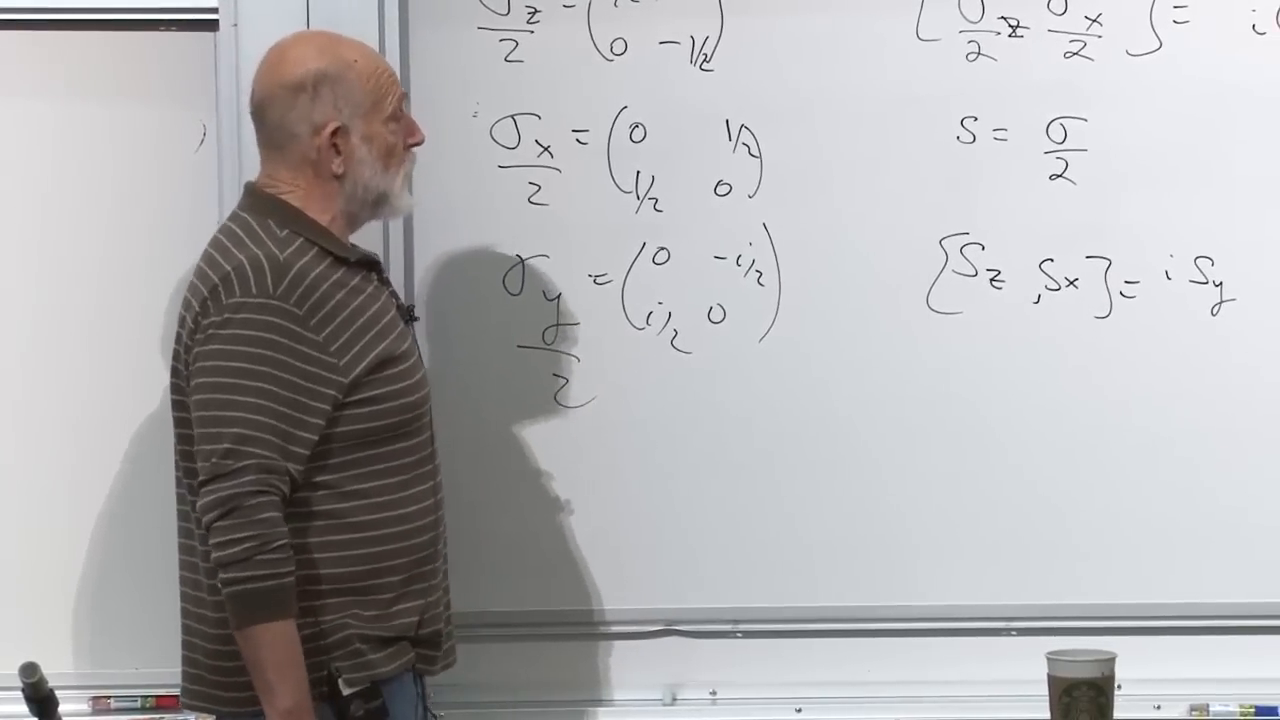
\includegraphics[width=0.9\linewidth]{lecture_04_frame_02.png}
\caption{In Einheiten, in denen \(\hbar=1\) gilt, sind die halben Pauli-Matrizen die Drehimpulsoperatoren für Spin einhalb und erfüllen \([S_z,S_x]=iS_y\).}
\lectureframe{00:55:41}
\end{figure}

Die beiden Eigenwertgleichungen für \(S_z\) lauten
\begin{equation}
S_z\lvert\pm\rangle
=\pm\frac{\hbar}{2}\lvert\pm\rangle.
\end{equation}
Äquivalent dazu ist die dimensionslose magnetische Quantenzahl
\begin{equation}
m_{s}=\pm\frac12,
\qquad
S_{z}\lvert m_{s}\rangle
=m_{s}\hbar\,\lvert m_{s}\rangle.
\end{equation}
Drehimpuls-Auf- und -Absteigeoperatoren verschieben \(m\) in ganzzahligen Schritten; daraus folgt jedoch nicht, dass jede Leiter durch null verlaufen muss. Multipletts mit ganzzahligem Drehimpuls enthalten ganzzahlige \(m\)-Werte, während Multipletts mit halbzahligen Drehimpulswerten halbzahlige Werte enthalten. Für Spin-einhalb umfasst die Leiter nur die beiden Zustände \(m_s=+1/2\) und \(m_s=-1/2\).

Diese beiden Zustände bilden das Spin-einhalb-Dublett. Elektronen, Myonen, Neutrinos und Quarks gehören zu den Teilchen, die durch solche Multipletts mit halbzahligem Spin beschrieben werden.

\section{Bahn- und Spin-Drehimpuls}

Es gibt nun zwei Arten von Drehimpuls. Der Bahndrehimpuls beschreibt die Bewegung relativ zu einem Ursprung:
\begin{equation}
\mathbf L=\mathbf R\times\mathbf P,
\end{equation}
\(\mathbf S\) ist dagegen intrinsischer Spin. Ihre Vektorsumme ist der Gesamtdrehimpuls:
\begin{equation}
\mathbf J=\mathbf L+\mathbf S.
\end{equation}

\begin{classroomqa}
\lecturetimestamp{00:56:49}
\audiencequestion{Wie lässt sich bei einem System mit dem Gesamtdrehimpuls \(\mathbf J\) sein Spin \(\mathbf S\) bestimmen?}
\lecturerresponse{Die Spin- und Bahndrehimpulsquantenzahlen werden gewöhnlich getrennt angegeben. Wenn \(L=0\) gilt, ist der gesamte Drehimpuls Spin. Andernfalls benötigt man die Quantisierungsregeln für die Addition von Drehimpulsen, die hier erst später behandelt werden.}
\end{classroomqa}

Die Additionsregeln gelten gleichermaßen für Bahndrehimpuls plus Spin, für zwei Spins oder für zwei Bahndrehimpulse. Das zusammengesetzte System besitzt eigene erlaubte Werte des Gesamtdrehimpulses; diese Regeln brauchen wir aber noch nicht.

\begin{classroomqa}
\lecturetimestamp{00:58:18}
\audiencequestion{Welche experimentellen Befunde führten zur Einführung des Spins?}
\lecturerresponse{Die Spektroskopie lieferte Hinweise, doch das Periodensystem bietet eine besonders anschauliche Motivation: Seine Schalenstruktur erfordert, dass Elektronen eine zusätzliche zweifach mögliche Eigenschaft besitzen.}
\end{classroomqa}

\section{Entartung des wasserstoffähnlichen Atoms und Schalenbesetzung}

Für den Bahndrehimpuls lautet die Eigenwertgleichung von \(L^{2}\)
\begin{equation}
L^{2}\lvert\ell,m\rangle
=\hbar^{2}\ell(\ell+1)\lvert\ell,m\rangle,
\end{equation}
Zu einem festen Wert von \(\ell\) gehören
\begin{equation}
2\ell+1
\end{equation}
magnetische Zustände, entsprechend \(m=-\ell,-\ell+1,\ldots,\ell\).

Das ideale nichtrelativistische Coulomb-Problem weist eine zusätzliche Entartung auf. Seine gebundenen Zustände haben negative Energien, die sich von unten null annähern; für die Zählung kommt es jedoch nur auf die Zuordnung der Niveaus zueinander an. Das erste Niveau mit \(\ell=1\) fällt mit dem nächsten Niveau mit \(\ell=0\) zusammen; das erste Niveau mit \(\ell=2\) kommt zur nächsten Hauptschale hinzu; und das Muster setzt sich fort.\footnote{\texttt{lecture\_04\_frame\_03.png}, \(01{:}02{:}01\); die vollständige Zuordnung der Hauptschalen wird von \(01{:}02{:}33\) bis \(01{:}04{:}10\) gezeigt.}

\begin{figure}[htbp]
\centering
\begin{tikzpicture}[x=1.55cm,y=1.0cm]
\draw[->] (-0.65,0) -- (-0.65,4.35);
\draw[->] (-0.85,0) -- (4.75,0);
\node at (-0.95,4.08) {\(E\)};
\node at (4.55,-0.28) {\(\ell\)};
\node at (0,-0.30) {\(0\)};
\node at (2,-0.30) {\(1\)};
\node at (4,-0.30) {\(2\)};

\draw (-0.20,0.75) -- (0.20,0.75);

\draw (-0.20,2.00) -- (0.20,2.00);
\foreach \dx in {-0.18,0,0.18}
  \draw (2+\dx-0.06,2.00) -- (2+\dx+0.06,2.00);

\draw (-0.20,3.15) -- (0.20,3.15);
\foreach \dx in {-0.18,0,0.18}
  \draw (2+\dx-0.06,3.15) -- (2+\dx+0.06,3.15);
\foreach \dx in {-0.32,-0.16,0,0.16,0.32}
  \draw (4+\dx-0.05,3.15) -- (4+\dx+0.05,3.15);

\node[anchor=west] at (0.35,0.75) {\(n=1\)};
\node[anchor=west] at (2.35,2.00) {\(n=2\)};
\node[anchor=west] at (4.40,3.15) {\(n=3\)};
\end{tikzpicture}
\caption{Die ersten drei idealen Coulomb-Schalen vereinigen Bahndrehimpulsmultipletts gleicher Hauptenergie: einen Zustand in der ersten Schale, \(1+3\) in der zweiten und \(1+3+5\) in der dritten.}
\lectureframe{01:02:01}
\end{figure}

In der Hauptschale \(n\) sind die erlaubten Bahndrehimpulsquantenzahlen\footnote{Dieser kompakte Bereich für \(\ell\) und die folgende Summe ergeben wieder die Zuordnungen der Niveaus sowie die Anzahlen \(1,4,9,16,\ldots\), die von \(01{:}02{:}33\) bis \(01{:}04{:}10\) angegeben werden. Der Anfang der Spektrumszeichnung ist bei \texttt{lecture\_04\_frame\_03.png} bei \(01{:}02{:}01\)zu sehen.}
\[
\ell=0,1,\ldots,n-1.
\]
Die Anzahl der räumlichen Zustände ist daher
\begin{equation}
\sum_{\ell=0}^{n-1}(2\ell+1)=n^{2},
\end{equation}woraus sich die Folge ergibt
\begin{equation}
1,\ 4,\ 9,\ 16,\ldots .
\end{equation}
Dies zählt nur die Bahndrehimpulszustände. Zu jedem räumlichen Zustand sind zwei Spinwerte möglich, sodass sich die entsprechenden idealisierten Gesamtzahlen ergeben:
\begin{equation}
2,\ 8,\ 18,\ 32,\ldots=2n^{2}.
\end{equation}

\section{Ausschlussprinzip und die zweifache Eigenschaft des Elektrons}

Betrachten wir zunächst Helium in der Näherung unabhängiger Elektronen. Sein Kern hat die doppelte Protonenladung, wodurch die wasserstoffähnlichen Energieniveaus skaliert werden und die Elektronen nach innen gezogen werden. Vernachlässigt man vorerst die Wechselwirkungen zwischen Elektronen--, können zwei Elektronen das niedrigste räumliche Orbital besetzen und so eine brauchbare erste Näherung für den Helium-Grundzustand ergeben.

Warum kann man nicht auch noch ein drittes Elektron dort unterbringen? Dadurch würde seine Orbitalenergie sinken, doch das geschieht nicht. Die Einschränkung ist das Pauli-Ausschlussprinzip: Keine zwei Elektronen dürfen denselben vollständigen Einteilchenzustand besetzen. Es wäre irreführend, dies als gewöhnliche abstoßende Kraft zu bezeichnen. Es handelt sich um eine Einschränkung der erlaubten Quantenzustände.

Hier scheint ein Widerspruch vorzuliegen. Die beiden Heliumelektronen besetzen tatsächlich dasselbe räumliche Orbital. Die Auflösung besteht darin, dass ein vollständiger Elektronenzustand mehr enthält als die Orbitalwellenfunktion. Er umfasst auch einen Freiheitsgrad mit zwei möglichen Werten. Nennen wir sie Spin-auf und Spin-ab. Ein Elektron im niedrigsten Orbital kann Spin-auf und das andere Spin-ab haben; ihre räumlichen Zustände stimmen überein, ihre vollständigen Quantenzustände aber nicht.

An dieser Stelle beginnt die Zählung mit Lithium und geht anschließend einen Schritt zurück. Dieser Rückschritt zeigt, warum sowohl das Ausschlussprinzip als auch der Spin notwendig sind. Stellen wir uns eine Ausschlussregel ganz ohne Spin vor. Dann könnte nur ein Elektron den niedrigsten räumlichen Zustand besetzen. Ein zweites Elektron müsste in einen der vier räumlichen Zustände der nächsten Hauptschale eintreten, sodass es mehrere Möglichkeiten für den Helium-Grundzustand gäbe, obwohl dieser beobachtbar eindeutig ist. Diese spinlose Fassung des Ausschlussprinzips ist falsch.

Berücksichtigen wir wieder die beiden Spinwerte. Zwei Elektronen füllen das niedrigste Orbital mit entgegengesetztem Spin. Ein drittes Elektron, wie bei neutralem Lithium, muss in die nächste Hauptschale eintreten. Diese Schale hat einen räumlichen Zustand mit \(\ell=0\) und drei räumliche Zustände mit \(\ell=1\). Vor Berücksichtigung des Spins gibt es also vier Möglichkeiten.

\begin{classroomqa}
\lecturetimestamp{01:14:58}
\audiencequestion{Wie ergeben die \(s\)- und \(p\)-Zustände acht Möglichkeiten in der ersten angeregten Schale?}
\lecturerresponse{Es gibt einen räumlichen Zustand mit \(\ell=0\) und drei mit \(\ell=1\), also insgesamt vier räumliche Zustände. Zu jedem sind zwei Spinwerte möglich, sodass sich insgesamt \(2(1+3)=8\) ergibt.}
\end{classroomqa}

Diese einfache Zählung erklärt die acht Einträge in der zweiten Zeile des Periodensystems. Sie ist bewusst idealisiert: Wie die spätere Diskussion zeigen wird, beeinträchtigen die Wechselwirkungen zwischen Elektronen-- das Bild unabhängiger wasserstoffähnlicher Schalen schon bald.

Die zweifache Eigenschaft lässt sich auch als Drehimpuls prüfen. Der Spin des Elektrons geht mit einem magnetischen Moment einher, sodass ein Magnetfeld den beiden Spinprojektionen unterschiedliche Energien verleiht. Ein Energieniveau, das bei verschwindendem Feld entartet war, spaltet sich in zwei auf, wie man es für ein kleines magnetisches Moment erwartet, das parallel oder antiparallel zum Feld ausgerichtet ist. Die Aufspaltung prüft, ob sich der zusätzliche zweifache Freiheitsgrad wie Drehimpuls verhält und nicht bloß wie eine beliebige binäre Kennzeichnung.

\section{Photonen, Elektronen und die Grenzen des Schalenmodells}

Teilchen folgen nicht alle derselben Besetzungsregel. Viele Photonen können dieselbe elektromagnetische Mode besetzen; eine klassische Lichtwelle lässt sich als Zustand mit einer großen Zahl von Photonen in dieser Mode verstehen. Elektronen verhalten sich anders: Das Ausschlussprinzip verhindert, dass sie sich in einem vollständigen Quantenzustand ansammeln. Dieser Gegensatz begründet die Unterscheidung zwischen den beiden Teilchenstatistiken.

\begin{classroomqa}
\lecturetimestamp{01:20:28}
\audiencequestion{Was gilt für einen freien Elektronenstrahl statt für Elektronen, die in Atomen gebunden sind?}
\lecturerresponse{Das Ausschlussprinzip gilt weiterhin: Die Elektronen können nicht alle denselben Quantenzustand einnehmen. Ein Laser kann viele Photonen in denselben Modus bringen, doch ein Elektronenstrahl lässt sich nicht auf diese Weise präparieren.}
\end{classroomqa}

Diese Einschränkung ist eine Eigenschaft der Elektronen und keine Besonderheit der atomaren Bindung.

\begin{classroomqa}
\lecturetimestamp{01:21:12}
\audiencequestion{Ist der Bahndrehimpuls speziell eine Drehung um einen Atomkern?}
\lecturerresponse{Der Drehimpuls ist bezüglich eines gewählten Ursprungs definiert. In einem Atom ist der Kern der natürliche Ursprung; ein freies Teilchen hat dagegen bezüglich des jeweils gewählten Ursprungs den Drehimpuls \(\mathbf R\times\mathbf P\).}
\end{classroomqa}

Bei jeder Betrachtung einer Rotation wählt man einen Punkt, um den die Rotation erfolgt. Ein Atom besitzt ein natürliches Zentrum, weil sein Kern das Zentrum des annähernd zentralen Potentials ist. Im freien Raum ist kein Ursprung ausgezeichnet, doch der Drehimpuls lässt sich weiterhin bezüglich eines beliebig gewählten Ursprungs berechnen.

\begin{classroomqa}
\lecturetimestamp{01:22:34}
\audiencequestion{Warum gibt es im Periodensystem wiederholt Reihen mit acht und dann mit achtzehn Elementen?}
\lecturerresponse{Das einfache Schalenmodell unabhängiger Elektronen erklärt das vollständige Muster nicht. Es versagt rasch, weil es die Wechselwirkungen zwischen den Elektronen vernachlässigt.}
\end{classroomqa}

Bei einem großen Atom wechselwirken die äußeren Elektronen sowohl mit einer beträchtlichen inneren Elektronenwolke als auch mit dem Kern. Es ist nicht mehr sinnvoll, jedes Elektron so zu behandeln, als bewege es sich unabhängig in einem ungeschirmten Coulomb-Feld.

\begin{classroomqa}
\lecturetimestamp{01:23:33}
\audiencequestion{Warum werden Atome nicht dramatisch größer, wenn weitere Elektronen hinzukommen?}
\lecturerresponse{Mit den zusätzlichen Elektronen kommen auch Protonen zum Kern hinzu. Die größere Kernladung zieht die inneren Elektronen nach innen, während diese inneren Elektronen den Kern abschirmen. In diesem einfachen Bild bewegt sich ein äußeres Valenzelektron dann in einer effektiven Ladung von ungefähr eins.}
\end{classroomqa}

Die erhöhte Kernladung zieht die innere Elektronenwolke zusammen. Bei einem Atom mit einem äußeren Valenzelektron heben sich Kern und innere Elektronen in großer Entfernung nahezu auf, sodass das Valenzelektron einem Feld ausgesetzt ist, das ungefähr dem einer positiven Elementarladung entspricht. Die Atomgröße nimmt daher nicht einfach proportional zur Zahl der Elektronen zu.

\begin{classroomqa}
\lecturetimestamp{01:24:49}
\audiencequestion{Ist die elektrische Abstoßung der Grund dafür, dass benachbarte Atome voneinander getrennt bleiben?}
\lecturerresponse{Nicht für sich allein. Das Pauli-Ausschlussprinzip bewirkt eine wichtige effektive Abstoßung, wenn sich Elektronenwolken überlappen, und bei vielen Atomen ist es der vorherrschende Grund dafür, dass sie einer weiteren Überlappung entgegenwirken.}
\end{classroomqa}

Die Pauli-Abstoßung ist eine effektive Folge des Ausschlussprinzips und kein zusätzliches Kraftgesetz.

\begin{classroomqa}
\lecturetimestamp{01:25:23}
\audiencequestion{Ist das Ausschlussprinzip ein eigenständiges Postulat?}
\lecturerresponse{In der nichtrelativistischen Quantenmechanik wird es als Postulat vorausgesetzt. In der relativistischen Quantentheorie gibt ihm der Spin--Statistik-Zusammenhang eine tiefergehende Begründung.}
\end{classroomqa}

\section{Identische Teilchen in klassischer und Quantenmechanik}

Bevor wir dieses Postulat formulieren, betrachten wir, wie identische Teilchen klassisch gezählt werden. Man bringe zwei Teilchen derselben Art in einer Menge von Kästen unter. Tragen die Teilchen insgeheim Namen---Harry und Sally---, dann scheint Harry im ersten Kasten und Sally im zweiten etwas anderes zu sein als Sally im ersten und Harry im zweiten.

Die klassische Mechanik lässt dieses Bild zu, selbst wenn die Bezeichnungen nicht deutlich genug sind, um sie zu erkennen. Man kann sich eine beliebig schwache Markierung auf jedem Teilchen vorstellen und ihre Bahnen dennoch als verschieden betrachten. In der klassischen statistischen Mechanik entscheidet man sich üblicherweise dafür, Vertauschungen identischer Teilchen nicht als neue Konfigurationen zu zählen. Für \(N\) Teilchen ergibt diese Konvention den bekannten Faktor \(1/N!\).

Die Quantenmechanik ist strenger. Identische Teilchen tragen keine verborgenen individuellen Kennzeichnungen, die sich prinzipiell verfolgen ließen. Zwei Elektronen sind als Elektronen vertauschbar. Ein Elektron gegen ein Photon auszutauschen ergäbe eine physikalisch andere Anordnung, da es sich um verschiedene Teilchenarten handelt. Durch die Vertauschung der beiden Elektronenplätze lässt sich jedoch nicht feststellen, welches Elektron tatsächlich welches war.

Ein Einteilchenzustand hat eine Wellenfunktion
\[
\psi(x)=\langle x\vert\psi\rangle.
\]
Für zwei Teilchen ist der Zustand eine Funktion zweier Ortsargumente:
\begin{equation}
\psi(x_{1},x_{2}).
\end{equation}
Die Indizes bezeichnen die beiden Plätze in der Beschreibung, nicht zwei Raumrichtungen. Ihr Betragsquadrat ist die gemeinsame Wahrscheinlichkeitsdichte für die Positionen.

\section{Der Vertauschungsoperator und das Statistikpostulat}

Vertauschen wir die beiden Teilchenplätze:
\begin{equation}
\psi(x_{1},x_{2})\longmapsto\psi(x_{2},x_{1}).
\end{equation}
In Anlehnung an die hier verwendete Notation bezeichnen wir den Vertauschungsoperator mit \(S\). Dabei steht \(S\) für den Austausch und nicht für den Spinvektor \(\mathbf S\). Seine Wirkung ist
\begin{equation}
(S\psi)(x_{1},x_{2})=\psi(x_{2},x_{1}).
\end{equation}
Eine allgemeine Funktion zweier Variablen muss nicht symmetrisch sein; diese Operation kann daher eine andere Wellenfunktion ergeben.

Zweimaliges Vertauschen stellt die ursprüngliche Reihenfolge wieder her:
\begin{equation}
S^{2}=I.
\end{equation}
Die Vertauschung ist umkehrbar und erhält die Skalarprodukte, sie wird also durch einen unitären Operator dargestellt. Ist \(\psi\) ein Eigenvektor von \(S\) mit dem Eigenwert \(\lambda\), dann gilt
\[
S^{2}\psi=\lambda^{2}\psi=\psi,
\]
und folglich
\begin{equation}
\lambda=\pm1.
\end{equation}

Diese Schlussfolgerung weist zwei Austauscheigenräume aus, besagt aber nicht, dass jede beliebige Zweiteilchen-Wellenfunktion bereits ein Eigenvektor von \(S\) ist. Jede solche Wellenfunktion lässt sich in ihre beiden Anteile zerlegen,\footnote{Diese Zerlegung ist eine redaktionelle algebraische Klarstellung der beiden durch \(S^{2}=I\) implizierten Eigenräume. Die aufgezeichnete Argumentation nennt die beiden Eigenwerte und führt anschließend das zusätzliche Statistikprinzip ein.}\begin{equation}
\psi_{\pm}=\frac12(I\pm S)\psi,
\end{equation}die folgende Beziehungen erfüllen:
\begin{equation}
S\psi_{\pm}=\pm\psi_{\pm}.
\end{equation}
Damit gilt:
\begin{align}
\psi_{+}(x_{2},x_{1})&=\psi_{+}(x_{1},x_{2}),\\
\psi_{-}(x_{2},x_{1})&=-\psi_{-}(x_{1},x_{2}).
\end{align}

Nun kommt ein zusätzliches Prinzip hinzu, das nicht allein aus \(S^{2}=I\) folgt. Bei identischen Teilchen einer festgelegten Teilchensorte liegen die erlaubten Zustände vollständig in einem dieser Austauschräume: Beim Austausch eines Teilchenpaars ergibt sich stets dieselbe Wellenfunktion oder stets ihr Negatives. Der Sektor \(+1\) ist symmetrisch, der Sektor \(-1\) antisymmetrisch. Die physikalische Deutung dieser beiden Möglichkeiten als die beiden Teilchenstatistiken ist der nächste Schritt und bleibt der folgenden Diskussion vorbehalten.

\chapter{Austauschsymmetrie, Spin und die beiden Minuszeichen}

\section{Schalenbesetzung und die Frage nach der Spin--Statistik}

Die Betrachtung des Schalenmodells beginnt mit zwei Eigenschaften der Elektronen. Ein Elektron hat den Spin eins halb, mit den beiden dimensionslosen Spinprojektionen
\begin{equation}
m_s=+\frac12,
\qquad
m_s=-\frac12,
\end{equation}
und Elektronen gehorchen dem Pauli-Ausschlussprinzip. Diese Tatsachen hängen zusammen, sind aber nicht dieselbe Aussage.

Der Ausdruck ``derselbe Zustand'' bedarf einer Präzisierung. Keine zwei Elektronen dürfen denselben vollständigen Einteilchenzustand besetzen. Zwei Elektronen können dennoch dasselbe räumliche Orbital teilen, wenn ihre Spinzustände verschieden sind. In der Näherung unabhängiger Elektronen für Helium besetzen beide Elektronen das niedrigste räumliche Orbital, eines mit Spin nach oben, das andere mit Spin nach unten. Genauer gesagt gehören die Alternativen ``das erste hat Spin nach oben und das zweite nach unten'' und ``das erste hat Spin nach unten und das zweite nach oben'' zu einem verschränkten Zweielektronen-Spinzustand.

Dies ist lediglich die alte Näherung des Schalenmodells. Sie vernachlässigt die Wechselwirkung zwischen den Elektronen und dient hier der einfachen Zählung. Bei Lithium besetzen die ersten beiden Elektronen das niedrigste räumliche Orbital mit entgegengesetztem Spin. Das dritte Elektron kann keinen dieser vollständigen Zustände einnehmen und muss ein höheres Orbital besetzen.

Als Nächstes folgt das vertraute Diagramm des Bahndrehimpulses. Die Bereiche mit
\begin{equation}
\ell=0,\qquad \ell=1,\qquad \ell=2
\end{equation}
heißen \(S\)-, \(P\)- und \(D\)-Zustände. Zu einem festen Wert von \(\ell\) gehören
\begin{equation}
2\ell+1
\end{equation}
Bahndrehimpulszustände, also
\begin{equation}
\ell=0\Rightarrow 1,
\qquad
\ell=1\Rightarrow 3,
\qquad
\ell=2\Rightarrow 5.
\end{equation}
Das Coulomb-Problem weist zusätzliche Entartungen auf: Radialzustände aus verschiedenen \(\ell\)-Sektoren können dieselbe Energie haben. Für die Betrachtung der Schalenbesetzung enthält die nächste Schale ein \(S\)-Orbital und drei \(P\)-Orbitale. Sie hat daher
\begin{equation}
1+3=4
\end{equation}
räumliche Zustände. Der Spin verdoppelt diese Zahl:
\begin{equation}
2(1+3)=8.
\end{equation}

Diese acht vollständigen Einteilchenzustände werden in der einfachen Abfolge von Lithium bis Neon aufgefüllt. Nach der abgeschlossenen Schale hat Natrium wieder ein äußeres Elektron; deshalb ähnelt es in diesem groben Bild Lithium. Um die Chemie geht es hier nicht. Entscheidend ist, dass halbzahliger Spin und Ausschluss gemeinsam auftreten.

Photonen bilden den Gegenfall. Sie haben ganzzahligen Spin und unterliegen keiner Ausschlussregel. Einer klassischen elektromagnetischen Welle entsprechen viele Photonen, die denselben Modus besetzen. Bosonen können sich in einem gemeinsamen Zustand ansammeln, während identische Fermionen einen vollständigen Zustand höchstens einmal besetzen können. Die Frage ist, ob diese beiden Zuordnungen auch andersherum möglich sein könnten: halbzahligen Spin ohne Ausschluss oder ganzzahligen Spin mit Ausschluss. In drei räumlichen Dimensionen lautet die Antwort gemäß der Spin--Statistik-Beziehung nein. Die vertraute Aussage bedarf in einer und zwei räumlichen Dimensionen einer Einschränkung; ein Beweis des feldtheoretischen Ergebnisses wird hier nicht versucht.

\begin{classroomqa}
\lecturetimestamp{00:11:48}
\audiencequestion{Gibt es eine Höchstzahl an Bosonen, die einen Zustand besetzen können?}
\lecturerresponse{Nein. Für Bosonen gibt es keine Besetzungsgrenze, und sie sammeln sich tendenziell im selben Zustand an.}
\end{classroomqa}

\section{Wellenfunktionen vieler Teilchen}

Dem Zusammenhang nähern wir uns über zwei Minuszeichen: eines stammt vom Austausch, das andere von der Rotation. Wir beginnen mit dem Austausch und lassen den Spin zunächst außer Betracht.

Sei \(x_i\) die Position des Teilchens \(i\). Der Index bezeichnet ein Teilchen und keine kartesische Komponente; die drei räumlichen Koordinaten werden in einem einzigen Symbol zusammengefasst: \(x_i\). Eine Ortsbasis für \(n\) Teilchen ist
\begin{equation}
\lvert x_1,x_2,\ldots,x_n\rangle.
\end{equation}
Für einen abstrakten Zustand \(\lvert\Psi\rangle\) lautet die Ortswellenfunktion
\begin{equation}
\psi(x_1,x_2,\ldots,x_n)
=
\langle x_1,x_2,\ldots,x_n\mid\Psi\rangle.
\end{equation}
Ihr Betragsquadrat,
\begin{equation}
\bigl\lvert\psi(x_1,x_2,\ldots,x_n)\bigr\rvert^2,
\end{equation}
ist die gemeinsame Wahrscheinlichkeitsdichte dafür, Teilchen \(1\) bei \(x_1\), Teilchen \(2\) bei \(x_2\) und so weiter zu finden.

Nehmen wir nun an, die Teilchen seien identisch. Stellen wir uns zunächst vor, ein Elektron sei blau und ein anderes rot angemalt. Dann ließe sich ``blau bei \(x_1\), rot bei \(x_2\)'' von ``blau bei \(x_2\), rot bei \(x_1\) unterscheiden.'' Tatsächliche Elektronen tragen keine solchen Farben oder individuellen Kennzeichnungen. Eine Vertauschung der Buchführungsindizes kann keine neue physikalische Anordnung erzeugen.

Eine globale Phase ändert weder Wahrscheinlichkeiten noch Erwartungswerte. Für einen Zustand mit bestimmtem Austauschverhalten kann die Ortswellenfunktion daher folgende Beziehung erfüllen:
\begin{equation}
\psi(x_2,x_1)=\eta\,\psi(x_1,x_2),
\qquad
\lvert\eta\rvert=1.
\end{equation}
Wendet man denselben Austausch zweimal an, erhält man die ursprünglichen Argumente zurück und es gilt
\begin{equation}
\eta^2=1,
\end{equation}
Die beiden möglichen Austauscheigenwerte sind somit
\begin{equation}
\eta=+1
\qquad\hbox{or}\qquad
\eta=-1.
\end{equation}

\editorialnote{Die Algebra des doppelten Austauschs legt die möglichen Eigenwerte erst fest, nachdem für einen Zustand ein bestimmtes Austauschverhalten vorausgesetzt wurde. Die weitergehende Einschränkung, dass die zulässigen Zustände einer festen Teilchensorte zu einem einzigen Austauschsektor gehören, ist eine physikalische Regel; sie folgt nicht allein aus \(\eta^2=1\). Dieselbe Einschränkung gilt für das folgende Ausschlussargument: Antisymmetrie impliziert Ausschluss, sobald der fermionische Sektor gewählt ist, aber die Algebra des Austauschs allein wählt diesen Sektor nicht aus.}

Bei Bosonen sind die zulässigen Wellenfunktionen symmetrisch,
\begin{equation}
\psi_B(x_1,x_2)=\psi_B(x_2,x_1),
\end{equation}
bei Fermionen dagegen antisymmetrisch,
\begin{equation}
\psi_F(x_1,x_2)=-\psi_F(x_2,x_1).
\end{equation}
Das Minuszeichen bleibt unsichtbar, wenn es den gesamten Zustand multipliziert, spielt aber eine Rolle, wenn Amplituden addiert werden. So hat die Austauschsymmetrie beobachtbare Folgen.

\section{Produkte, Summen und Ausschluss}

Betrachten wir zunächst zwei Teilchen, die demselben Einteilchenorbital \(\psi_0\) zugeordnet sind. Ihr Produkt lautet
\begin{equation}
\psi_0(x_1)\psi_0(x_2).
\end{equation}
Beim Austausch der Teilchenkoordinaten ergibt sich
\begin{equation}
\psi_0(x_2)\psi_0(x_1)
=
\psi_0(x_1)\psi_0(x_2).
\end{equation}
Wellenfunktionswerte sind Zahlen, keine Operatoren; die Faktoren kommutieren also. Das Produkt für denselben Zustand ist symmetrisch. Es ist eine zulässige bosonische Form, kann aber keine zwei identischen Fermionen beschreiben.

Ordnen wir die Teilchen nun verschiedenen Einteilchenorbitalen zu:
\begin{equation}
\psi_0(x_1)\psi_1(x_2).
\end{equation}
Beim Austausch erhält man
\begin{equation}
\psi_0(x_2)\psi_1(x_1).
\end{equation}
Für verschiedene Funktionen ist das vertauschte Produkt im Allgemeinen weder der ursprüngliche Ausdruck noch dessen Negatives. Das bloße Produkt besitzt daher keine der erforderlichen Austauschsymmetrien. Damit ist nicht ausgeschlossen, dass ein Teilchen \(\psi_0\) besetzt und ein anderes \(\psi_1\). Es bedeutet, dass der Zweiteilchenzustand die beiden Zuordnungen kombinieren muss.

Die symmetrische Kombination lautet
\begin{equation}
\psi_B^{(01)}(x_1,x_2)
\propto
\psi_0(x_1)\psi_1(x_2)
+
\psi_0(x_2)\psi_1(x_1),
\end{equation}
die antisymmetrische Kombination
\begin{equation}
\psi_F^{(01)}(x_1,x_2)
\propto
\psi_0(x_1)\psi_1(x_2)
-
\psi_0(x_2)\psi_1(x_1).
\end{equation}
Proportionalitätszeichen genügen, da für das Austauschargument keine Normierung erforderlich ist. Beide Zustände enthalten je ein Teilchen in jedem Orbital; sie unterscheiden sich nur darin, wie die beiden ununterscheidbaren Zuordnungen kombiniert werden.

Lassen wir nun die Orbitale zusammenfallen. Die bosonische Kombination wird zu
\begin{align}
\psi_B^{(00)}(x_1,x_2)
&\propto
\psi_0(x_1)\psi_0(x_2)
+
\psi_0(x_2)\psi_0(x_1)\\
&=
2\psi_0(x_1)\psi_0(x_2),
\end{align}
und ist von null verschieden. Die fermionische Kombination ergibt
\begin{align}
\psi_F^{(00)}(x_1,x_2)
&\propto
\psi_0(x_1)\psi_0(x_2)
-
\psi_0(x_2)\psi_0(x_1)\\
&=0.
\end{align}
Mit der antisymmetrischen Austauschregel folgt der Ausschluss: Es gibt keinen von null verschiedenen antisymmetrischen Zustand, in dem sich beide Fermionen im selben Einteilchenzustand befinden.

Bei einem Zustand aus vielen Teilchen gilt die Regel für jede Vertauschung zweier Argumente. Eine Vertauschung lässt eine bosonische Wellenfunktion unverändert und kehrt bei einer fermionischen ihr Vorzeichen um. Wiederholt man dieselbe Vertauschung, ist das in beiden Fällen trivial. Erstaunlich ist, dass ein einzelner Austausch zwar keine beobachtbaren Teilchenkennzeichnungen verändert, aber das Vorzeichen eines fermionischen Zustands umkehrt.

\section{Der Spin in der vollständigen Teilchenkennzeichnung}

Der Spin lässt sich nun mit einer kleinen Änderung wieder einbeziehen. Eine Einteilchenamplitude hängt sowohl von der Position als auch von einer diskreten Spinbezeichnung ab:
\begin{equation}
\psi(x,\sigma),
\end{equation}
wobei \(\sigma=+1\) oder \(-1\) das gewählte Ergebnis von \(\sigma_z\) bezeichnet. Das Betragsquadrat ist die gemeinsame Wahrscheinlichkeitsdichte für die angegebene Position und Spinbezeichnung.

Für viele Teilchen lautet die Wellenfunktion
\begin{equation}
\psi(x_1,\sigma_1;\,x_2,\sigma_2;\,\ldots).
\end{equation}
Beim Austausch wird alles vertauscht, was zu den beiden Teilchen gehört, nicht nur ihre Positionen:
\begin{align}
\psi_B(x_1,\sigma_1;\,x_2,\sigma_2)
&=
+\psi_B(x_2,\sigma_2;\,x_1,\sigma_1),\\
\psi_F(x_1,\sigma_1;\,x_2,\sigma_2)
&=
-\psi_F(x_2,\sigma_2;\,x_1,\sigma_1).
\end{align}
Dies ist die präzise Form der eingangs gemachten Aussage zum Schalenmodell. Zwei Elektronen können dasselbe räumliche Orbital nur dann teilen, wenn ihre vollständigen Zustände einschließlich des Spins verschieden sind.

\begin{classroomqa}
\lecturetimestamp{00:34:33}
\audiencequestion{Ist die Austauschsymmetrie ein Beispiel für die Permutationsgruppe?}
\lecturerresponse{Ja. Der Austausch von Teilchen ist eine Permutation, und das Plus- oder Minus-Transformationsgesetz liefert eine Darstellung der Permutationsgruppe.}
\end{classroomqa}

\begin{classroomqa}
\lecturetimestamp{00:35:12}
\audiencequestion{Warum ist die Zweiteilchenkonstruktion ein Produkt und keine Summe der Einteilchenwellenfunktionen?}
\lecturerresponse{Eine Summe beschreibt ein Teilchen in einer Superposition. Ein Produkt gehört zum Zweiteilchen-Tensorproduktraum und beschreibt ein Teilchen, das jeweils einem der beiden Einteilchenzustände zugeordnet ist.}
\end{classroomqa}

Der Austausch der vollständigen Teilchenkennzeichnungen ist auf der folgenden Tafel dargestellt.\footnote{Die Reihenfolge der Orts--Spin-Bezeichnungen wurde anhand des lesbaren Tafelbilds und der umgebenden Erläuterung von 00:33:43 bis 00:34:25 rekonstruiert.}
\begin{figure}[htbp]
\centering
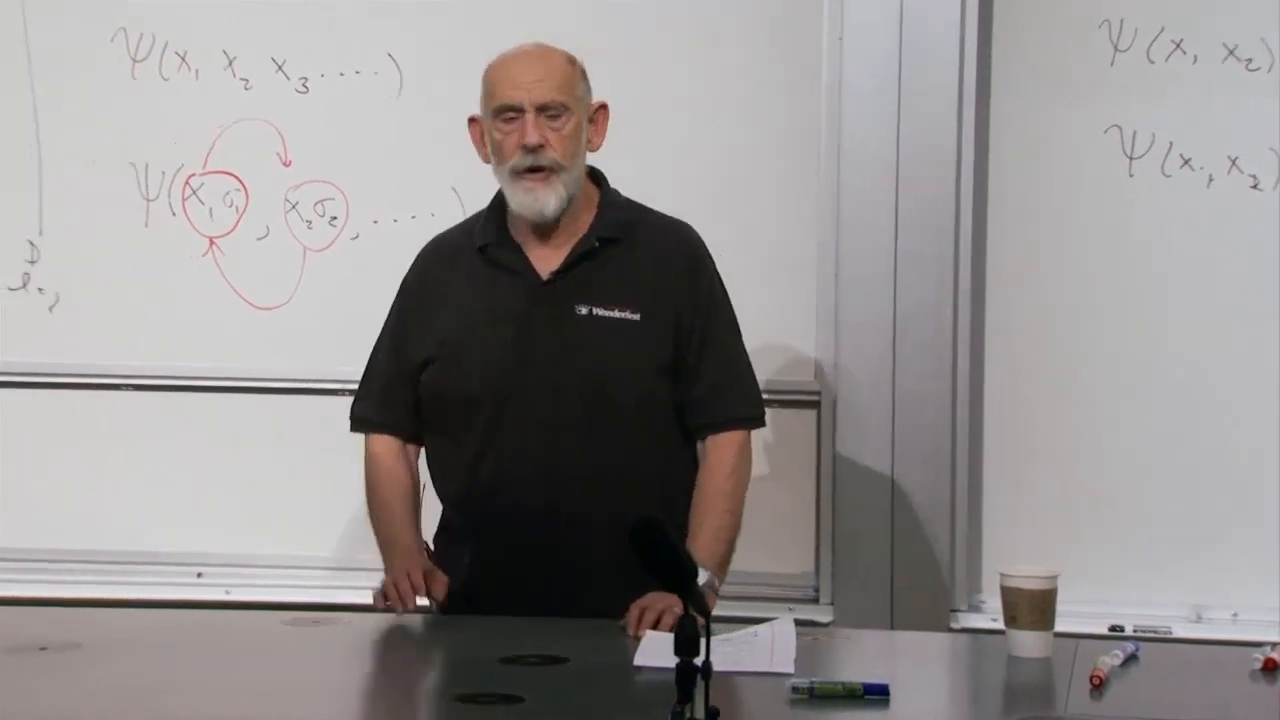
\includegraphics[width=0.9\linewidth]{lecture_05_frame_03.png}
\caption{Beim Austausch zweier identischer Teilchen werden ihre vollständigen Orts--Spin-Bezeichnungen vertauscht. Ein bosonischer Zustand bleibt unverändert, während ein fermionischer sein Vorzeichen ändert.}
\lectureframe{00:35:25}
\end{figure}

Hier kommen zwei verschiedene Arten von Linearität zum Einsatz. Für ein Teilchen ist
\begin{equation}
\alpha\psi_0(x)+\beta\psi_1(x)
\end{equation}
eine Superposition zweier Alternativen. Für zwei Teilchen ist
\begin{equation}
\psi_0(x_1)\psi_1(x_2)
\end{equation}
eine Produktamplitude in einem Raum mit zwei Teilchenkoordinaten. Durch Symmetrisierung oder Antisymmetrisierung wird dieses Produkt mit seinem vertauschten Gegenstück kombiniert.

\begin{classroomqa}
\lecturetimestamp{00:36:13}
\audiencequestion{Führt der Teilchenaustausch zu einem Interferenzeffekt?}
\lecturerresponse{Ja. Die verschwindende fermionische Amplitude für denselben Zustand lässt sich als destruktive Interferenz der beiden ausgetauschten Beiträge verstehen.}
\end{classroomqa}

\begin{classroomqa}
\lecturetimestamp{00:37:13}
\audiencequestion{Hat Pauli den Ausschluss mithilfe desselben Symmetriearguments hergeleitet?}
\lecturerresponse{Pauli ging von einer empirischen Tatsache aus und fand einen mathematischen Rahmen, in dem sie sich ausdrücken ließ. Zunächst leitete er den Ausschluss nicht aus einer fundamentaleren Theorie her.}
\end{classroomqa}

Die Antisymmetrie liefert den mathematischen Rahmen, in dem sich die empirische Ausschlussregel ausdrücken lässt.

\begin{classroomqa}
\lecturetimestamp{00:39:01}
\audiencequestion{Hängt die Interferenz beim Teilchenaustausch mit der Interferenz zwischen alternativen Wegen zusammen?}
\lecturerresponse{Ja. In einer möglichen Geschichte passieren die beiden Teilchen einander, ohne sich zu kreuzen; in einer anderen kreuzen sie sich und gelangen so zu den vertauschten Endorten. Bei Bosonen addieren sich die Amplituden, bei Fermionen können sie sich auslöschen.}
\end{classroomqa}

Der Austausch liefert das erste Minuszeichen. Die Rotation liefert das zweite.

\section{Das zweite Minuszeichen: Rotation um \texorpdfstring{\(2\pi\)}{2 pi}}

Eine vollständige Rotation scheint nichts zu bewirken. Jede gewöhnliche geometrische Richtung kehrt nach einem Winkel von \(2\pi\) zu ihrer Ausgangslage zurück. Zurückkehren müssen jedoch die Wahrscheinlichkeiten und Erwartungswerte. Der Zustandsvektor selbst kann mit einer globalen Phase zurückkehren, ebenso wie beim Austausch.

\begin{classroomqa}
\lecturetimestamp{00:42:12}
\audiencequestion{Um welche Achse wird rotiert, und ist der Generator der Bahndrehimpuls, der Spin oder beides?}
\lecturerresponse{Man kann eine äußere Achse wählen; im Folgenden nehmen wir die \(z\)-Achse. Der Generator ist der Gesamtdrehimpuls, einschließlich der orbitalen und der Spinbeiträge. Der Spin selbst muss nicht entlang der gewählten Achse zeigen.}
\end{classroomqa}

\editorialnote{In dieser Diskussion werden die Formeln für den Drehimpuls mit \(\hbar=1\) geschrieben; \(m\) ist daher der dimensionslose Eigenwert von \(J_z\).}

Sei \(\psi(\theta)\) der Zustand, der entsteht, wenn der Rotationsparameter einen Winkel von \(\theta\) durchläuft. In der hier verwendeten Konvention gilt
\begin{equation}
J_z\psi(\theta)
=
-i\frac{\partial}{\partial\theta}\psi(\theta).
\end{equation}
Für einen Zustand mit bestimmtem \(J_z\) gilt
\begin{equation}
J_z\psi(\theta)=m\psi(\theta).
\end{equation}
Durch Kombination der Gleichungen erhält man
\begin{equation}
-i\frac{\partial}{\partial\theta}\psi(\theta)
=
m\psi(\theta),
\end{equation}
mit der Lösung
\begin{equation}
\psi(\theta)=e^{im\theta}\psi(0).
\end{equation}

Die zulässigen Werte von \(m\) sind ganzzahlig oder halbzahlig. Daher gilt
\begin{equation}
\psi(2\pi)
=
\begin{cases}
+\psi(0), & m\in\mathbb Z,\\[4pt]
-\psi(0), & m\in\mathbb Z+\tfrac12.
\end{cases}
\end{equation}
Nach einer weiteren vollständigen Drehung gilt in beiden Fällen
\begin{equation}
\psi(4\pi)=\psi(0)
\end{equation}
Dies ist das zweite Minuszeichen: Ein Zustand aus einem Drehimpulsmultiplett mit halbzahligem Drehimpuls ändert bei einer Rotation um \(2\pi\) sein Vorzeichen.

Das Vorzeichen ändert \(\lvert\psi\rvert^2\) nicht und bleibt daher unsichtbar, wenn es den gesamten Zustand multipliziert. Dennoch wird eine Rotation um \(2\pi\) bei einem Zustand mit halbzahligem Spin nicht durch die Identität dargestellt. Beobachtbar wird der Unterschied, wenn das Vorzeichen relativ zu einer anderen kohärenten Amplitude auftritt.

\section{Die Wege mit \texorpdfstring{\(2\pi\) und \(4\pi\)}{2 pi und 4 pi}}

Der Unterschied zwischen \(2\pi\) und \(4\pi\) lässt sich ohne weitere Algebra sichtbar machen. Halten Sie eine Tasse in einer Hand und drehen Sie sie um eine volle Umdrehung, ohne sie loszulassen. Die Tasse kehrt in ihre ursprüngliche Ausrichtung zurück, aber der Arm ist verdreht. Drehen Sie sie eine weitere Umdrehung, lässt sich der Arm in seine ursprüngliche Lage zurückbringen, ohne die Drehbewegung der Tasse umzukehren.

Eine verwandte Konstruktion verwendet eine Kugel in einer Schachtel, die mit Schnüren an der Schachtel befestigt ist. Dreht man die Kugel um \(2\pi\), entsteht ein Wirrwarr. Im gewöhnlichen dreidimensionalen Raum lässt sich das Gewirr, das einer Drehung um \(4\pi\) entspricht, entwirren. Entscheidend ist nicht nur die Endausrichtung der Kugel, sondern der Weg durch den Raum der Rotationen.

\begin{classroomqa}
\lecturetimestamp{00:54:22}
\audiencequestion{Wenn die Kugel zweimal um dieselbe Achse gedreht wird, lassen sich die Schnüre dann wirklich entwirren? Erfordert das eine weitere räumliche Dimension?}
\lecturerresponse{Der Weg mit \(4\pi\) lässt sich im gewöhnlichen dreidimensionalen Raum entwirren. Die Zeit parametrisiert die Bewegung; sie ist keine weitere räumliche Richtung. Ein Weg mit \(2\pi\) lässt sich auf diese Weise nicht entwirren, ein Weg mit \(4\pi\) dagegen schon.}
\end{classroomqa}

Die Demonstrationen unterscheiden einen nichttrivialen Weg mit \(2\pi\) von einem entwirrbaren Weg mit \(4\pi\), ohne eine formale Theorie der Rotationsgruppe zu entwickeln.

\section{Austausch und Rotation im Gürtelbild}

Nun stehen die beiden Minuszeichen nebeneinander. Der Austausch zweier identischer Fermionen ändert das Vorzeichen ihrer gemeinsamen Wellenfunktion. Auch eine Rotation eines Zustands mit halbzahligem Spin um \(2\pi\) ändert sein Vorzeichen. Ein Gürtel stellt eine geometrische Beziehung zwischen diesen beiden Vorgängen her.

Ordnen Sie den Gürtel so an, dass seine beiden unteren Enden vertauscht sind. Anders betrachtet weist derselbe Gürtel eine Verdrehung um \(2\pi\) auf. Führt man den Austausch zusammen mit der Rotation um \(2\pi\) aus, verschwindet die Verdrehung und der Gürtel bleibt unverdrillt. Der kombinierte Vorgang lässt sich stetig auf nichts tun zurückführen.\footnote{Die Beobachtung zum Austausch und zur--Rotation wird in der Vorlesung David Finkelstein zugeschrieben. Da die Quellenaufzeichnung keine bestimmte Veröffentlichung nennt, wird der Name hier nur als diese Zuschreibung beibehalten.}

\begin{classroomqa}
\lecturetimestamp{01:01:12}
\audiencequestion{Beschreibt dies nur die Einbettung des Gürtels in den Raum oder auch die Topologie von Teilchen?}
\lecturerresponse{Der Gürtel lässt sich als Teilchengeschichte in der Raumzeit auffassen. Zeigt die Zeit nach oben, liefert ein Querschnitt teilchenartige Objekte. Paare werden erzeugt, ein Objekt wird um \(2\pi\) gedreht und zwei identische Objekte werden vertauscht. In dieser Geschichte heben sich die Rotations- und Austauschphasen auf.}
\end{classroomqa}

An dieser Geschichte lässt sich die Phasenbilanz explizit ablesen. Beginnen wir ohne Teilchen. An zwei voneinander getrennten Orten wird jeweils ein Teilchen--Antiteilchen-Paar erzeugt, sodass es zu einem Zwischenzeitpunkt vier Teilchen gibt. Während ein Teilchen um \(2\pi\) gedreht wird, werden an anderer Stelle in der Konfiguration zwei identische Teilchen vertauscht. Die vollständige Geschichte lässt sich in die elementare Geschichte umformen, in der ein Paar erzeugt und später wieder vernichtet wird. In der hier betrachteten Vorzeichenbilanz hat diese triviale Geschichte keine zusätzliche Phase. Bezeichnen \(\eta_{\mathrm{rot}}\) und \(\eta_{\mathrm{ex}}\) die beiden Vorzeichen, lässt sich die mündlich beschriebene Aufhebung knapp so schreiben:\footnote{Diese Phasengleichung hält die Aufhebung fest, die von 01:06:50 bis 01:07:18 beschrieben wird; die Vorlesung stellt die Konstruktion als anschaulich, nicht als strengen Beweis dar.}
\begin{equation}
\eta_{\mathrm{rot}}\eta_{\mathrm{ex}}=1.
\end{equation}

\begin{classroomqa}
\lecturetimestamp{01:03:34}
\audiencequestion{Lässt sich der Austausch mit Rotationen verknüpfen, indem sich beide Teilchen um \(\pi\) bewegen und anschließend neu ausrichten?}
\lecturerresponse{Diese Konstruktion könnte verwandte Mathematik widerspiegeln, verwendet aber zwei getrennte Rotationen um \(\pi\). Der hier analysierte Vorgang umfasst eine Rotation um \(2\pi\); die beiden Argumente sind also nicht identisch.}
\end{classroomqa}

Das Argument setzt voraus, dass teilchenartige Objekte erzeugt und vernichtet werden können. In einer Theorie mit ewigen Teilchen hätte es nicht diese Form. Es wird auch nicht als Standardbeweis des Spin--Statistik-Theorems vorgelegt. Es soll einen topologischen Grund dafür veranschaulichen, dass die Vorzeichen von Austausch und Rotation zusammenpassen.

\section{Klumpen, Spiegelbilder und Vernichtung}

Die Konstruktion lässt sich mit lokalisierten Feldkonfigurationen wiederholen. Nehmen wir an, ein oder mehrere Felder nehmen fast überall ihre Vakuumwerte an, weisen aber in einem kleinen Bereich eine nichtverschwindende Form und Struktur auf. Eine solche lokalisierte Konfiguration ist ein Klumpen.

Erzeugen wir nun eine zweite Konfiguration als das passende Spiegelbild der ersten. Nennen wir die eine Teilchen und die andere Antiteilchen. Bringen wir sie zusammen. Entsprechende Teile der Feldkonfigurationen treffen aufeinander und heben sich gegenseitig auf. In einem Zwischenstadium können manche Teile der Klumpen bereits verschwunden sein, während andere noch bestehen. Durch Fortsetzen der Verformung verschwindet auch die übrige Struktur, und die Felder kehren zur Vakuumkonfiguration zurück. Zwei entgegengesetzt angeordnete Verdrehungen in einem Gürtel veranschaulichen dasselbe: Schiebt man sie zusammen, entwirren sie sich.

Der Vorgang lässt sich rückwärts ablaufen. Aus dem leeren Raum können ein Klumpen und sein Spiegelbild entstehen. Man kann zwei solcher Paare erzeugen, einen Klumpen um \(2\pi\) drehen, zwei identische Klumpen vertauschen und die Paare wieder vernichten. Dieselbe Aufhebung von Austausch und--Rotation gilt dann auch hier. Dies bleibt eine heuristische Erweiterung der Konstruktion und ist kein Theorem über jede lokalisierte Anregung.

\begin{classroomqa}
\lecturetimestamp{01:11:30}
\audiencequestion{Gibt es physikalische Realisierungen solcher klumpenartigen Feldkonfigurationen?}
\lecturerresponse{Ja. Beispiele sind Kerne in Skyrmion-artigen Beschreibungen, magnetische Monopole und andere teilchenartige Anregungen von Feldern.}
\end{classroomqa}

Das Bild der gespiegelten Klumpen macht die Verallgemeinerung verständlich. Entscheidend ist nicht, dass das Objekt ursprünglich ein elementares Punktteilchen war, sondern dass eine teilchenartige Anregung und ihr Partner kontinuierlich erzeugt, zusammengebracht und vernichtet werden können. Diese Eigenschaft legt eine allgemeinere Beziehung zwischen Rotations- und Austauschverhalten nahe.

\begin{classroomqa}
\lecturetimestamp{01:16:12}
\audiencequestion{Bedeutet Spin eins halb, dass der Zustand nur die Hälfte der üblichen Rotationsphase annimmt?}
\lecturerresponse{Die Phase lautet in dieser Konvention \(e^{im\theta}\). Für halbzahliges \(m\) ergibt eine Rotation um \(2\pi\) den Faktor \(-1\), während eine Rotation um \(4\pi\) den Faktor \(+1\) ergibt.}
\end{classroomqa}

\section{Ein globales Vorzeichen und ein Nullresultat}

Lässt sich das Minuszeichen einer Rotation um \(2\pi\) beobachten? Beginnen wir mit einem Experiment, bei dem das nicht möglich ist. Fangen wir ein Elektron in einem Magnetfeld ein, lassen seinen Spin dem Feld folgen, während die Apparatur langsam um \(2\pi\) gedreht wird, und geben das Elektron anschließend in eine Interferenzapparatur frei. Vergleichen wir dies mit demselben Ablauf ohne Rotation.

Die Rotation verändert den Zustand gemäß
\begin{equation}
\psi\longmapsto-\psi,
\end{equation}
Doch das Minuszeichen multipliziert den gesamten Zustand. Alle Wahrscheinlichkeiten bleiben unverändert; das abschließende Interferenzmuster enthält daher keine Information darüber, ob die vorherige Rotation stattgefunden hat. Dies ist ein Nullresultat: Eine gemeinsame Phase hat nichts, womit sie interferieren könnte.

\begin{classroomqa}
\lecturetimestamp{01:20:01}
\audiencequestion{Warum muss die Drehung des Magnetfelds langsam erfolgen?}
\lecturerresponse{Der Spin muss dem rotierenden Magnetfeld weiter folgen. Wird das Feld zu schnell bewegt, bleibt der Spin nicht an es gekoppelt.}
\end{classroomqa}

\section{Ein Elektron in zwei kohärenten Zweigen}

Das Vorzeichen wird beobachtbar, wenn man es relativ macht. Schicken wir ein Elektron durch einen Strahlteiler. Ein Teil seiner Wellenfunktion folgt dem einen Weg, ein anderer Teil einem zweiten:
\begin{equation}
\psi(x)=\psi_1(x)+\psi_2(x).
\end{equation}
Es handelt sich um ein Elektron, nicht um zwei Elektronen. Es ist eine kohärente Superposition zweier Alternativen. Diese Unterscheidung muss klar bleiben: Die beiden Wellenpakete sind keine zwei unabhängigen Teilchen.

Führen wir die beiden Wellenpakete in getrennte Bereiche mit Magnetfeldern. Drehen wir das Feld in einem Bereich um \(2\pi\) und lassen das andere unverändert. Für einen Zustand mit halbzahligem Spin gilt
\begin{equation}
\psi_1(x)+\psi_2(x)
\longmapsto
\psi_1(x)-\psi_2(x),
\end{equation}
wobei der gedrehte Zweig mit \(2\) bezeichnet wird. Nun ist das Vorzeichen relativ. Wenn sich die beiden Wellenpakete später überlagern, wird aus der Addition eine Subtraktion. Ein Punkt konstruktiver Interferenz kann zu einem Punkt destruktiver Interferenz oder sogar zu einem Knoten werden.

\begin{classroomqa}
\lecturetimestamp{01:23:46}
\audiencequestion{Was wird gedreht, wenn es nur ein Elektron, aber zwei Zweige der Wellenfunktion gibt?}
\lecturerresponse{Das Elektron befindet sich in einer kohärenten Superposition zweier lokalisierter Alternativen. Ein Zweig wird gedreht, der andere nicht. Öffnet man die Kästen, um herauszufinden, welche Alternative eingetreten ist, zerstört diese Messung die Interferenz.}
\end{classroomqa}

Beim Öffnen der Kästen würde sich zeigen, dass sich das einzige Elektron in einem der beiden Kästen befindet. Ohne diese Messung bleiben beide Amplituden im Zustand erhalten. Wiederholt man das Experiment, baut sich das Interferenzmuster nach und nach auf, eine Detektion nach der anderen. An einem durch das relative Minuszeichen erzeugten Knoten wird kein Elektron detektiert.

\section{Magnetische Präzession und Doppelspaltinterferenz}

Ein praktischeres schematisches Verfahren ersetzt das sehr langsame Experiment mit den Kästen. Teilen wir eine kohärente Elektronenwelle auf zwei Wege auf. Auf einem Weg durchquert das Elektron einen Magnetfeldbereich, wobei sein Spin zunächst quer zum Feld steht. Daraufhin präzediert der Spin. Durch geeignete Wahl der Feldstärke und der Durchlaufzeit kann der Spin in diesem Zweig eine vollständige Drehung um \(2\pi\) ausführen, während der andere Zweig keine solche Drehung erfährt.\footnote{Die Vorlesung berichtet, dass ein verwandtes Spinorphasen-Experiment durchgeführt worden sei, und erläutert dessen Prinzip; die Quellenaufzeichnung nennt jedoch weder eine Veröffentlichung noch eine bestimmte Apparatur. Die Darstellung hier beschränkt sich daher auf die in der Vorlesung beschriebene Konstruktion.}

\begin{classroomqa}
\lecturetimestamp{01:27:05}
\audiencequestion{Wie lässt sich der Weg des einzelnen Elektrons bestimmen?}
\lecturerresponse{Das ist nicht möglich, ohne das Experiment zu zerstören. Jede Messung, die aufzeichnet, welchen Weg das Elektron genommen hat, zerstört die Interferenz.}
\end{classroomqa}

\begin{classroomqa}
\lecturetimestamp{01:27:50}
\audiencequestion{Was genau ist ein Zweig der Wellenfunktion, und wie erzeugt der Strahlteiler zwei Zweige?}
\lecturerresponse{Ein Zweig ist ein entlang eines Weges lokalisiertes Wellenpaket. Der Strahlteiler formt die einlaufende Welle zu zwei räumlich getrennten Wellenpaketen; elektrische oder magnetische Felder können diese auf unterschiedlichen Wegen führen.}
\end{classroomqa}

Abgesehen vom Magnetfeldbereich entspricht dies dem Doppelspaltexperiment. Eine einlaufende Elektronenwelle teilt sich in zwei Wellenpakete. Die auslaufenden Wellen breiten sich in einen gemeinsamen Detektionsbereich aus, wo sich ihre Amplituden überlagern. Ohne relative Rotation können sich die zentralen Amplituden addieren. Eine Spinrotation um \(2\pi\) auf einem der Wege kehrt eine Amplitude um und kann bewirken, dass sich dieselben Beiträge auslöschen.

\begin{classroomqa}
\lecturetimestamp{01:30:46}
\audiencequestion{Wie kann es Interferenz geben, wenn das Elektron durch getrennte Röhren oder Spalte läuft?}
\lecturerresponse{Die abschließende Detektion lässt den Weg nicht erkennen. Die beiden auslaufenden Wellenamplituden breiten sich aus und überlagern sich am Detektor. Herauszufinden, welchen Weg das Elektron genommen hat, würde die Interferenz zerstören.}
\end{classroomqa}

\begin{classroomqa}
\lecturetimestamp{01:33:22}
\audiencequestion{Muss der Durchmesser der Röhre oder des Spalts in der Größenordnung der Elektronenwellenlänge liegen?}
\lecturerresponse{Bei einer wörtlichen, auf Beugung beruhenden Doppelspaltrealisierung muss die Öffnung klein genug sein, um die erforderliche Ausbreitung zu bewirken. Die beschriebene Apparatur ist schematisch und keine praktische Konstruktion.}
\end{classroomqa}

\begin{classroomqa}
\lecturetimestamp{01:33:44}
\audiencequestion{Würde eine entsprechende \(2\pi\)-Drehung der Photonenpolarisation das Interferenzmuster unverändert lassen?}
\lecturerresponse{Ja. Photonen haben ganzzahligen Spin, daher führt eine vollständige Drehung um \(2\pi\) nicht zum fermionischen Minuszeichen.}
\end{classroomqa}

\begin{classroomqa}
\lecturetimestamp{01:34:12}
\audiencequestion{Worin weicht das praktische Experiment geringfügig von der idealisierten Version ab?}
\lecturerresponse{Bei der idealisierten Anordnung wird der Spin adiabatisch gedreht. In der Beschreibung des praktischen Experiments bewegt sich das Elektron durch einen Magnetfeldbereich, und sein Spin präzediert schneller; die gemessene Phase ist jedoch weiterhin die einer Drehung um \(2\pi\).}
\end{classroomqa}

Die langsame Anordnung macht die Idee anschaulich, indem sie sicherstellt, dass der Spin dem Feld ohne zusätzliche Bewegung folgt. Bei der Präzession entsteht dasselbe relative Vorzeichen dynamisch. In beiden Versionen müssen die beiden Wege ununterscheidbar werden, bevor ein Interferenzmuster auftreten kann.

\begin{classroomqa}
\lecturetimestamp{01:36:15}
\audiencequestion{Müssen die beiden Zweige nach dem Strahlteiler wieder zusammengeführt werden?}
\lecturerresponse{Ja. Die austretenden Wellenpakete müssen sich überlappen oder sich über einen gemeinsamen Detektionsbereich ausbreiten, damit ihre Amplituden ein Interferenzmuster bilden können.}
\end{classroomqa}

\begin{classroomqa}
\lecturetimestamp{01:38:12}
\audiencequestion{Ist dieses Rotationsexperiment mit einem Elektron eine Folge des Pauli-Ausschlussprinzips?}
\lecturerresponse{Nein. Es gibt nur ein Elektron. Das Experiment misst die Spinorphase bei einer Drehung, nicht den Ausschluss zweier Fermionen aus demselben Zustand.}
\end{classroomqa}

\section{Austauschinterferenz und relative Drehung}

Ein Austauschvorzeichen ließe sich mit derselben allgemeinen Methode nachweisen, auch wenn die vorgeschlagene Apparatur komplizierter ist. Man beginnt mit zwei Elektronen und spaltet ihre gemeinsame Wellenfunktion in zwei kohärente Zweige auf. Es gibt weiterhin nur zwei Elektronen, nicht vier: Das Elektronenpaar nimmt den einen oder den anderen Weg. In einem Zweig werden die beiden Elektronen vertauscht, im anderen nicht. Nachdem die Zweige wieder zusammengeführt worden sind, zeigt sich das fermionische Austauschvorzeichen als relative Phase und kann die Interferenz verändern.

Der letzte Vorschlag vergleicht die beiden Minuszeichen direkt. Ein Zweig erhält die fermionische Austauschphase, während der andere die entsprechende Phasenänderung bei einer Drehung um \(2\pi\) erfährt. Beide Phasen sind \(-1\), daher hebt sich ihre relative Wirkung auf.\footnote{Die Aufzeichnung zwischen 01:40:26 und 01:41:15 zeigt eindeutig eine Austauschphase, eine Phasenänderung bei einer Drehung um \(2\pi\) und deren Aufhebung; die genaue Zuordnung der Drehung lässt sich aus der verfügbaren Tonaufnahme jedoch nicht rekonstruieren.} Die Vorlesung stellt dies als vorgeschlagenes Gedankenexperiment dar und sagt, dass es nach Kenntnis des Vortragenden nicht durchgeführt worden war.

\begin{classroomqa}
\lecturetimestamp{01:41:34}
\audiencequestion{Würde die Beobachtung einer Austauschphase die Ununterscheidbarkeit der beiden Elektronen infrage stellen?}
\lecturerresponse{Nein. Quantenmechanische Ununterscheidbarkeit ist subtiler als klassische Gleichheit. Sie lässt zu, dass der Zustandsvektor beim Austausch sein Vorzeichen ändert, obwohl kein beobachtbares Merkmal die Teilchen unterscheidet.}
\end{classroomqa}

Es gibt noch eine letzte Einschränkung. Eine Drehung einer gesamten isolierten Welt um \(2\pi\) ergäbe nur eine gemeinsame Phase, die sich durch kein internes Experiment nachweisen ließe. Im nachweisbaren Experiment wird ein kohärenter Zweig relativ zu einem anderen gedreht. Beobachtet wird daher kein absolutes Vorzeichen, sondern die durch ein relatives Vorzeichen erzeugte Interferenz.

\chapter{Oszillatoren, Besetzungszahlen und das erste Quantenfeld}

Die Quantenfeldtheorie ist unser Rahmen für praktisch die gesamte bekannte nichtgravitative Physik. Diese Aussage darf nicht mit der Behauptung verwechselt werden, jedes Problem lasse sich lösen. Ein Wasserstoffatom ist noch handhabbar; bei einem Atom wie Bor wird die Rechnung bereits viel schwieriger, und ein Mensch liegt weit jenseits dessen, was sich mit einer realistischen feldtheoretischen Rechnung erfassen lässt. Der Rahmen mag fundamental sein, während seine Gleichungen überwältigend schwierig bleiben.

Wir nähern uns dem Thema daher auf die elementarste mögliche Weise. Das Gebiet wird manchmal als \emph{zweite Quantisierung} bezeichnet, doch der Name wird wenig bedeuten, bis wir den nötigen Formalismus aufgebaut haben. Der kürzeste Weg beginnt nicht mit einem relativistischen Feld, sondern mit dem harmonischen Oszillator. Federn sind nicht der entscheidende Punkt. Es geht um die Algebra der Erzeugungs- und Vernichtungsoperatoren. Wiederholt man diese Algebra für viele Moden, bedeutet ein Erzeugungsoperator nicht länger bloß ``einen Oszillator um eine Stufe anheben'', sondern ganz wörtlich ``ein Teilchen erzeugen.''

\section{Der Oszillator als Algebra}

Für einen einzelnen Oszillator sei \(a^\dagger\) der Operator, der die Anregung erhöht, und \(a\) derjenige, der sie erniedrigt. Die Schreibweisen \(a_+\) und \(a_-\) sind gleichwertig; die Dagger-Notation nimmt jedoch die in der Feldtheorie verwendete Sprache vorweg. Der Grundzustand erfüllt
\begin{equation}
a|0\rangle=0,
\end{equation}
und der Zahloperator ist
\begin{equation}
N=a^\dagger a,
\qquad
N|n\rangle=n|n\rangle.
\end{equation}
Die beiden Leiteroperatoren sind zueinander adjungiert, und ihr wesentlicher Kommutator lautet
\begin{equation}
[a,a^\dagger]=1.
\label{eq:l06-single-commutator}
\end{equation}
Diese kleine Algebra macht fast den ganzen Oszillator aus.

\(a\) und \(a^\dagger\) lassen sich als geeignete Linearkombinationen von Ort und Impuls darstellen. Die genaue Konvention hängt von der Normierung von \(x\), \(p\), \(m\) und \(\omega\) ab; die hier nützliche, von dieser Wahl unabhängige Aussage lautet, dass \(a^\dagger a\) den quadratischen Oszillator-Hamiltonoperator bis auf die additive Grundzustandsenergie rekonstruiert. Somit gilt
\begin{equation}
H=\hbar\omega\left(N+\frac12\right).
\end{equation}
Für die vorliegende Diskussion lassen wir den konstanten Term weg und verwenden
\begin{equation}
H=\hbar\omega N.
\label{eq:l06-one-oscillator-hamiltonian}
\end{equation}
Die Frequenz gibt an, welchen Preis eine Anregung hat. Eine Erhöhung von \(n\) um eins kostet \(\hbar\omega\); eine Erniedrigung von \(n\) um eins setzt denselben Betrag frei.

\section{Viele unabhängige Oszillatoren}

Betrachten wir nun viele Oszillatoren und kennzeichnen sie durch \(i\). Dieses Zeichen ist lediglich ein Index und nicht die imaginäre Einheit. Es kann endlich oder unendlich viele Moden geben. Eine Ansammlung unabhängiger Federn liefert ein Bild; die Normalmoden einer idealen Violinsaite ein anderes. Für die Anwendungen in der Feldtheorie ist der Fall mit unendlich vielen Moden entscheidend.

Unabhängigkeit hat eine operatorielle Bedeutung. Operatoren, die zu tatsächlich unabhängigen Teilsystemen gehören, kommutieren. Andernfalls könnten die zugehörigen Größen nicht unabhängig voneinander gemessen werden, und die Systeme wären von vornherein nicht unabhängig. Daher gilt
\begin{align}
[a_i,a_j]&=0, \\
[a_i^\dagger,a_j^\dagger]&=0, \\
[a_i,a_j^\dagger]&=\delta_{ij}.
\label{eq:l06-many-commutators}
\end{align}
Für \(i\ne j\) kommutiert alles, was zu den beiden Moden gehört. Für \(i=j\) reduziert sich die letzte Zeile auf Gleichung~\eqref{eq:l06-single-commutator}.

Jeder Oszillator hat seinen eigenen Zahloperator und im Allgemeinen auch seine eigene Frequenz:
\begin{equation}
N_i=a_i^\dagger a_i,
\qquad
H=\sum_i\hbar\omega_i N_i.
\label{eq:l06-many-hamiltonian}
\end{equation}
Ein gemeinsamer Eigenzustand wird durch die vollständige Liste
\begin{equation}
|n_1,n_2,n_3,\ldots\rangle,
\qquad n_i=0,1,2,\ldots.
\label{eq:l06-occupation-ket}
\end{equation}
gekennzeichnet. Die ganze Zahl \(n_i\) heißt \emph{Besetzungszahl} des \(i\)-ten Oszillators. Bislang ist das nur eine Bezeichnung. Bald wird sie die Zahl der Teilchen zählen, die einen Einteilchenzustand besetzen, und der Name wird wörtlich zu verstehen sein.

Der Zustand, in dem jede Besetzungszahl null ist, lautet
\begin{equation}
|0\rangle\equiv|0,0,0,\ldots\rangle,
\qquad a_i|0\rangle=0\quad\text{for every }i.
\label{eq:l06-oscillator-vacuum}
\end{equation}

\begin{classroomqa}
\lecturetimestamp{00:15:27}
\audiencequestion{Entspricht eine unendliche Familie von Oszillatoren dem Kontinuum der Moden eines Systems wie einer Violinsaite?}
\lecturerresponse{Ja, bei der idealisierten Saite. Eine reale Saite besteht aus Atomen, sodass hinreichend kurze Wellenlängen schließlich auf eine mikroskopische Abschneideskala stoßen. Das Kontinuumsmodell regt dennoch die unendliche Modenfamilie an, die in der Feldtheorie verwendet wird.}
\end{classroomqa}

\section{Warum die Leiterkoeffizienten Quadratwurzeln sind}

Die Wirkung von \(a^\dagger\) muss einen Eigenzustand von \(N\) auf den nächsten Eigenzustand abbilden, doch die Normierung lässt einen Koeffizienten offen:
\begin{equation}
a^\dagger|n\rangle=c_n|n+1\rangle.
\label{eq:l06-unknown-coefficient}
\end{equation}

\begin{figure}[htbp]
\centering
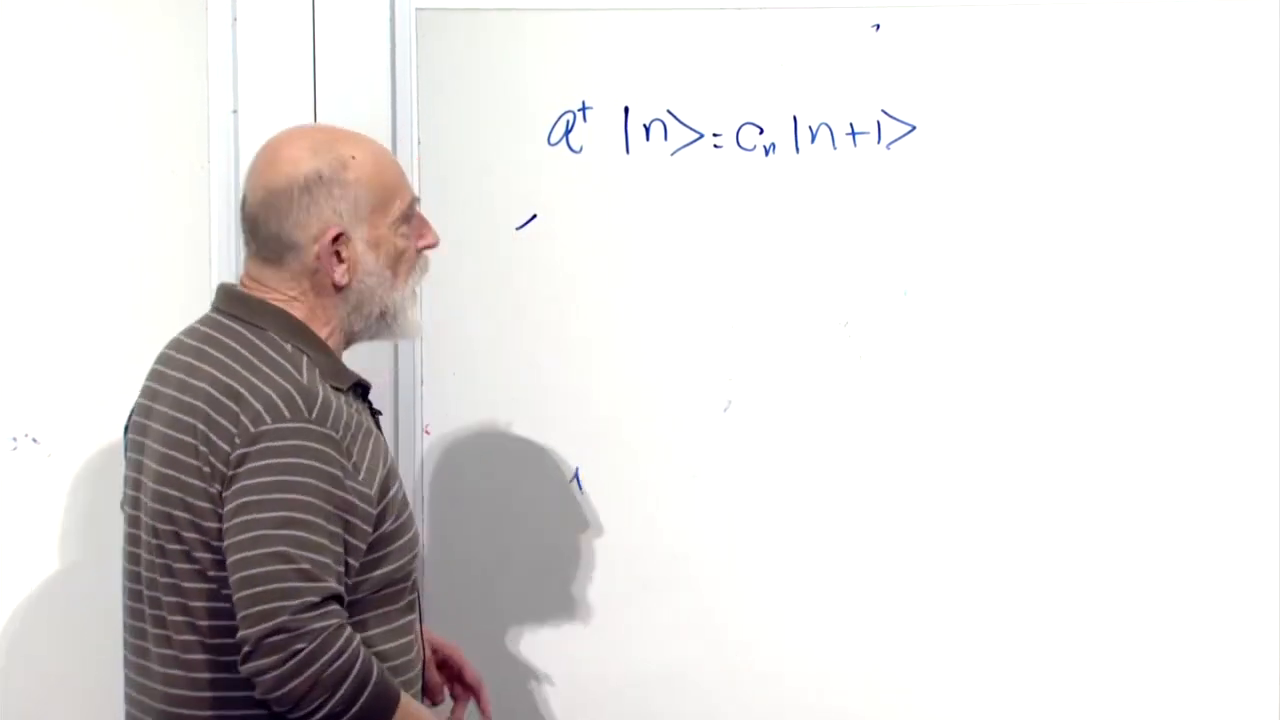
\includegraphics[width=0.9\linewidth]{lecture_06_frame_01.png}
\caption{Der Leiterkoeffizient wird eingeführt, bevor seine Normierung hergeleitet wird. Die Tafelgleichung ist in Gleichung~\eqref{eq:l06-unknown-coefficient} wiedergegeben.}
\lectureframe{00:19:38}
\end{figure}

Wir wählen die Phasenkonvention, in der \(c_n\) reell ist. Hermitesche Konjugation ergibt
\begin{equation}
\langle n|a=c_n\langle n+1|.
\end{equation}
Multipliziert man die beiden Beziehungen und verwendet normierte Basiszustände, so folgt
\begin{align}
c_n^2
&=\langle n|aa^\dagger|n\rangle \\
&=\langle n|(a^\dagger a+1)|n\rangle \\
&=\langle n|(N+1)|n\rangle \\
&=n+1.
\end{align}
Folglich gilt
\begin{equation}
a^\dagger|n\rangle=\sqrt{n+1}\,|n+1\rangle.
\label{eq:l06-raising-rule}
\end{equation}

\begin{classroomqa}
\lecturetimestamp{00:22:35}
\audiencequestion{Warum darf man \(\langle n+1|n+1\rangle=1\) setzen, bevor man \(c_n\) bestimmt?}
\lecturerresponse{Die Eigenvektoren werden von Anfang an als normierte Basis gewählt. Ihre Normierung legt die Normierung von \(a^\dagger|n\rangle\) nicht fest; genau diese noch offene Information steckt im Koeffizienten \(c_n\).}
\end{classroomqa}

Die Regel für den Vernichtungsoperator folgt auf dieselbe Weise:
\begin{equation}
a|n\rangle=\sqrt n\,|n-1\rangle.
\label{eq:l06-lowering-rule}
\end{equation}
Für \(n=0\) verschwindet der Koeffizient automatisch, sodass die Regel auch \(a|0\rangle=0\) einschließt. Bei mehreren Moden verändert der Operator nur die Besetzungszahl in seinem eigenen Eintrag:
\begin{align}
a_i^\dagger|n_1,\ldots,n_i,\ldots\rangle
&=\sqrt{n_i+1}\,|n_1,\ldots,n_i+1,\ldots\rangle, \\
a_i|n_1,\ldots,n_i,\ldots\rangle
&=\sqrt{n_i}\,|n_1,\ldots,n_i-1,\ldots\rangle.
\label{eq:l06-multimode-ladders}
\end{align}
Die übrigen Einträge bleiben unverändert.

\section{Eine Wellenfunktion ist kein Quantenfeld}

Bevor wir ein Feld definieren, müssen wir es von der vertrauten Wellenfunktion unterscheiden. Drei Gegenüberstellungen ordnen den Übergang.

Erstens ist eine Einteilchen-Wellenfunktion
\begin{equation}
\psi(x)=\langle x|\psi\rangle
\end{equation}
eine Darstellung eines Zustandsvektors. Sie ist selbst keine Observable. Wir messen Ort, Impuls, Drehimpuls und weitere Operatoren; die Wellenfunktion liefert die Amplituden, aus denen sich die Wahrscheinlichkeiten dieser Messergebnisse berechnen lassen.

Zweitens hängt eine Vielteilchen-Wellenfunktion von den Orten aller Teilchen ab. Für zwei Teilchen, deren Ortsvektoren vorläufig mit \(x\) und \(y\) bezeichnet seien, gilt
\begin{equation}
\psi(x,y)=\langle x,y|\psi\rangle.
\end{equation}
Hier kennzeichnen \(x\) und \(y\) zwei verschiedene Teilchen; sie sind nicht die kartesischen \(x\)- und \(y\)-Komponenten eines einzigen Ortsvektors. Bei \(N\) Teilchen wird der Zustand dargestellt durch
\begin{equation}
\psi(x_1,x_2,\ldots,x_N).
\end{equation}

Drittens beschreibt diese Wellenfunktion eine feste Teilchenzahl. Eine Wellenfunktion für fünfzehn Teilchen hat fünfzehn Ortsargumente und gehört zu einem Hilbertraum für fünfzehn Teilchen. Für sich allein beschreibt sie keinen Prozess, bei dem sich die Teilchenzahl von fünfzehn auf vierzehn oder sechzehn ändert.

Ein Quantenfeld kehrt diese Merkmale um. Es ist ein Operator statt eines Zustands, hängt von einem räumlichen Punkt \(x\) ab und wirkt auf einen Zustandsraum, der alle Teilchenzahlsektoren enthält. Die Wendung ``ein Punkt'' meint einen frei variierbaren Ortsvektor. Sie bedeutet nicht, dass \(x\) ein einzelner Zahlenwert zugewiesen wurde.

Eine Einschränkung wird später wichtig sein. Das weiter unten eingeführte Feld \(\Psi(x)\) ist nicht hermitesch und daher im strengen Sinn selbst keine Observable. Seine hermiteschen Kombinationen sind Observablen. Die vorläufige Aussage, ein Feld sei messbar, wird also präzisiert und nicht verworfen: Felder sind operatorwertige Funktionen, und ihre hermiteschen Kombinationen stellen messbare Größen dar.

\begin{classroomqa}
\lecturetimestamp{00:36:52}
\audiencequestion{Wenn das Feld eine Funktion des Ortes ist, darf dieser Ort dann variieren? Und was ist aus dem \(y\) in der Zweiteilchen-Wellenfunktion geworden?}
\lecturerresponse{Der Punkt \(x\) durchläuft den gesamten Raum. ``Ein Ort'' bedeutet, dass der Operator ein räumliches Argument hat, nicht dass dieses Argument festliegt. In \(\psi(x,y)\) bezeichnen die Symbole \(x\) und \(y\) die Orte zweier Teilchen; gleichwertig kann man sie als \(x_1\) und \(x_2\) schreiben. Sie sind nicht zwei kartesische Komponenten des Feldarguments.}
\end{classroomqa}

\begin{classroomqa}
\lecturetimestamp{00:38:15}
\audiencequestion{Wie hängen die Beschreibungen durch die Wellenfunktion für feste Teilchenzahl und durch Felder zusammen, und beschreiben sie unterschiedliche Teilchenarten?}
\lecturerresponse{Der Zusammenhang ist die zentrale Konstruktion, die noch aussteht. Es handelt sich um Teilchen derselben Art. In dieser Vorlesung betrachten wir Bosonen; für Fermionen ist eine andere Algebra erforderlich.}
\end{classroomqa}

\section{Ein Teilchen in einem Kasten}

Kehren wir vorübergehend zur gewöhnlichen Einteilchen-Quantenmechanik zurück. Wir bringen ein Teilchen in einem eindimensionalen Kasten unter. Bei nur einem Teilchen ist die Unterscheidung zwischen Boson und Fermion unerheblich: Es gibt kein zweites identisches Teilchen, mit dem man Austausch oder Ausschluss prüfen könnte.

Seien
\begin{equation}
\psi_1(x),\ \psi_2(x),\ \psi_3(x),\ldots
\end{equation}
die Energieeigenfunktionen. Die niedrigste Mode ist die glatteste Welle, die an den Wänden verschwindet. Die nächste Mode hat einen inneren Knoten, und höherenergetische Moden schwingen schneller. Für den idealen unendlich tiefen Potentialkasten der Breite \(L\) ist eine praktische normierte Basis
\begin{equation}
\psi_i(x)=\sqrt{\frac{2}{L}}\sin\!\left(\frac{i\pi x}{L}\right),
\qquad 0<x<L.
\label{eq:l06-box-basis}
\end{equation}
Die explizite Sinusformel ist eine Standardrealisierung der qualitativen Skizze an der Tafel; das folgende Argument erfordert lediglich eine vollständige Orthonormalbasis von Einteilchenzuständen.

\begin{figure}[htbp]
\centering
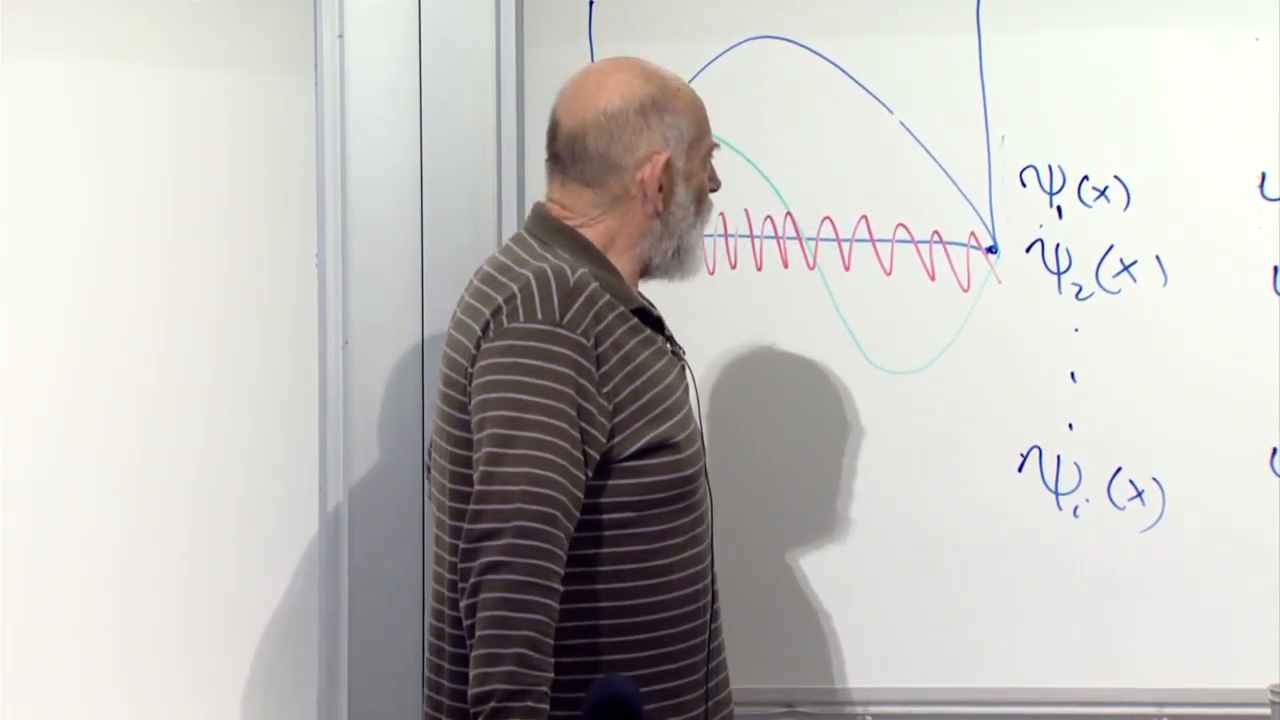
\includegraphics[width=0.9\linewidth]{lecture_06_frame_03.png}
\caption{Einteilchenmoden des Kastens, nach steigender Energie geordnet. Die erste Mode hat keinen inneren Knoten, die zweite einen, und die nicht gezeigten höheren Moden schwingen zunehmend schneller.}
\lectureframe{00:43:10}
\end{figure}

Dieselbe Struktur lässt sich ohne die Verdeckung durch die Live-Tafel neu zeichnen:
\begin{figure}[htbp]
\centering
\begin{tikzpicture}[x=1cm,y=1cm]
  \draw[thick] (0,0) -- (0,3.8);
  \draw[thick] (7,0) -- (7,3.8);
  \draw[gray!55] (0,2.75) -- (7,2.75);
  \draw[gray!55] (0,1.35) -- (7,1.35);
  \draw[blue!75!black,thick,domain=0:7,samples=120]
    plot (\x,{2.75+0.62*sin(180*\x/7)});
  \draw[teal!70!black,thick,domain=0:7,samples=120]
    plot (\x,{1.35+0.55*sin(360*\x/7)});
  \node[right] at (7.15,3.15) {$\psi_1(x)$};
  \node[right] at (7.15,1.70) {$\psi_2(x)$};
  \node at (3.5,0.45) {$\vdots\quad \psi_i(x)$};
\end{tikzpicture}
\caption{Eine saubere Rekonstruktion der qualitativen Skizze der Kastenmoden. Die vertikale Verschiebung trennt die Eigenfunktionen zur besseren Lesbarkeit; sie ist keine zusätzliche physikalische Koordinate.}
\end{figure}

Der Index \(i\) kennzeichnet einen Einteilchenzustand, nicht ein Teilchen und auch nicht die Zahl der Knoten. Bei der Kastenbasis ist \(i\) zufällig um eins größer als die Zahl der inneren Knoten. Jeder Zustand hat eine Energie \(\varepsilon_i\). In der Notation der Vorlesung können wir diese Energie als \(\hbar\omega_i\) schreiben oder, nach Setzen von \(\hbar=1\), einfach als \(\omega_i\).

\begin{classroomqa}
\lecturetimestamp{00:39:01}
\audiencequestion{War die frühere Annahme der Unabhängigkeit exakt, und könnte der Index \(i\) die möglichen Zustände eines Elektrons in einem Atom kennzeichnen?}
\lecturerresponse{Für die Konstruktion mit unabhängigen Moden ist die Kommutativität verschiedener Moden exakt. Der Index kann Einteilchenzustände eines Atoms kennzeichnen. Wenn die Teilchen jedoch miteinander wechselwirken, ist der einfache Hamiltonoperator unabhängiger Moden nicht mehr die ganze Beschreibung.}
\end{classroomqa}

\begin{classroomqa}
\lecturetimestamp{00:40:34}
\audiencequestion{Ist das Teilchen im Kasten ein Boson?}
\lecturerresponse{Das kann sein, doch bei einem Teilchen spielt die Statistik keine Rolle. Ausschluss und Austausch werden erst bei mehr als einem identischen Teilchen relevant.}
\end{classroomqa}

\section{Von Kastenmoden zum Fock-Raum}

Lassen wir nun eine beliebige Anzahl identischer Bosonen im Kasten zu. Eine Anzahl \(n_1\) kann \(\psi_1\) besetzen, eine Anzahl \(n_2\) kann \(\psi_2\) besetzen und so weiter. Ein Basiszustand ist daher
\begin{equation}
|n_1,n_2,n_3,\ldots\rangle.
\end{equation}
Dies ist genau die Notation, die bereits für viele Oszillatoren verwendet wurde. Die Übereinstimmung ist strukturell: Jedem Einteilchenzustand wird ein Oszillator zugeordnet, und die Anregungszahl des Oszillators wird mit der Zahl der Teilchen identifiziert, die diesen Zustand besetzen.

Bosonen sind hier wesentlich, denn jedes \(n_i\) kann eine beliebige nichtnegative ganze Zahl sein. Bei Fermionen kann jeder Einteilchenzustand leer oder einfach besetzt sein, niemals doppelt; daher lässt sich die gewöhnliche Oszillatoralgebra nicht unverändert verwenden.

Die Operatoren lassen sich nun durch ihre Wirkung auf die Besetzungszahlbasis definieren. Der Operator \(a_i^\dagger\) erzeugt ein Teilchen im Einteilchenzustand \(i\); \(a_i\) vernichtet eines:
\begin{align}
a_i^\dagger|n_1,\ldots,n_i,\ldots\rangle
&=\sqrt{n_i+1}\,|n_1,\ldots,n_i+1,\ldots\rangle, \\
a_i|n_1,\ldots,n_i,\ldots\rangle
&=\sqrt{n_i}\,|n_1,\ldots,n_i-1,\ldots\rangle.
\end{align}
Das ist keine nachträglich eingeführte Analogie. So sind die bosonischen Erzeugungs- und Vernichtungsoperatoren auf dieser Basis definiert. Da die Basis den Raum aufspannt, legt die Definition durch Linearität ihre Wirkung auf jeden Zustand fest.

\begin{classroomqa}
\lecturetimestamp{00:47:11}
\audiencequestion{Sind \(n_1,n_2,n_3\) die Quantenzustände?}
\lecturerresponse{Die Bezeichnungen \(1,2,3,\ldots\) kennzeichnen die Einteilchenzustände. Die Symbole \(n_1,n_2,n_3,\ldots\) geben die Anzahl der Teilchen an, die diese Zustände besetzen. Die Unterscheidung zwischen Zustandsbezeichnung und zugehöriger Besetzungszahl im Blick zu behalten, ist die wichtigste Notationsaufgabe.}
\end{classroomqa}

\subsection{Was die Quadratwurzel bewirkt}

Der Faktor \(\sqrt{n_i+1}\) steht weder für ein zusätzliches Teilchen noch für einen eigenen physikalischen Prozess. Er sorgt für die richtige Normierung und Algebra des Operators. Für eine Mode gilt
\begin{align}
a a^\dagger|n\rangle
&=a\bigl(\sqrt{n+1}\,|n+1\rangle\bigr) \\
&=(n+1)|n\rangle,
\end{align}
während
\begin{equation}
a^\dagger a|n\rangle=n|n\rangle.
\end{equation}
Ihre Differenz ist daher \(|n\rangle\), wie es \([a,a^\dagger]=1\) verlangt. Die beiden Leiteroperatoren sind grob gesprochen jeweils von der Größenordnung \(\sqrt n\), denn ihr Produkt ergibt den Zahloperator, der von der Größenordnung \(n\) ist.

\begin{classroomqa}
\lecturetimestamp{00:47:52}
\audiencequestion{Welche konkrete physikalische Bedeutung hat der Quadratwurzelfaktor?}
\lecturerresponse{Er dient in erster Linie der mathematischen Normierung. Er stellt sicher, dass die Besetzungszustände normiert sind, dass \(a^\dagger a\) den Eigenwert \(n\) hat und dass die Leiteroperatoren den Oszillatorkommutator erfüllen. Manchmal ist die Mathematik selbst die Bedeutung, die man braucht.}
\end{classroomqa}

\begin{classroomqa}
\lecturetimestamp{00:52:25}
\audiencequestion{Sind die Erzeugungs- und Vernichtungsoperatoren allein durch ihre Eigenschaften und ihre Wirkung auf die Basis definiert worden?}
\lecturerresponse{Ja. Definitionen müssen nicht aus einem grundlegenderen Bild hervorgehen. Ihr Wert zeigt sich an ihren Konsequenzen. Definiert man die Wirkung auf einer vollständigen Basis, sind die Operatoren überall festgelegt, und diese Definitionen reproduzieren die gewünschten Kommutationsrelationen.}
\end{classroomqa}

\begin{classroomqa}
\lecturetimestamp{00:53:22}
\audiencequestion{Warum lässt \(a_i\) ein Teilchen verschwinden, statt es lediglich in einen anderen Zustand zu versetzen?}
\lecturerresponse{Denn \(a_i\) ist so definiert, dass es die Besetzung des Zustands \(i\) erniedrigt. Die nützlichere Frage ist nicht, warum eine Definition gilt, sondern warum sie nützlich ist. Sie ist nützlich, weil Emission und Absorption Operatoren erfordern, die die Teilchenzahl ändern: Bei der Emission von Strahlung wird ein Photon erzeugt, bei seiner Absorption wird es vernichtet.}
\end{classroomqa}

Der von allen Besetzungszahlzuständen aufgespannte Raum heißt \emph{Fock-Raum}. Er enthält das Vakuum, jeden Einteilchenzustand, jeden Zweiteilchenzustand und so weiter, ohne feste obere Grenze:
\begin{equation}
\mathcal F=\mathcal H_0\oplus\mathcal H_1\oplus\mathcal H_2\oplus\cdots.
\label{eq:l06-fock-space}
\end{equation}
Die Direktsummenschreibweise macht explizit, was die gewöhnliche Wellenfunktion für \(N\) Teilchen nicht ausdrückte: Alle Teilchenzahlsektoren gehören zu einem einzigen Zustandsraum.

\begin{classroomqa}
\lecturetimestamp{00:54:56}
\audiencequestion{Legen Definitionen der Operatoren auf den Besetzungszahl-Eigenvektoren ihre Wirkung auf beliebigen Vektoren fest, und folgen daraus die Oszillatorkommutatoren?}
\lecturerresponse{Genau. Die Besetzungsvektoren bilden eine Basis, sodass die Linearität die Definition auf den gesamten Fock-Raum erweitert. Die bosonischen Kommutationsrelationen lassen sich durch Anwendung auf diese Basis überprüfen. Jeder Einteilchenzustand entspricht einem Oszillator, dessen Besetzungszahl der Teilchenzahl in diesem Zustand entspricht.}
\end{classroomqa}

\subsection{Das Vakuum und der freie Hamiltonoperator}

Das Fock-Vakuum ist der Zustand, in dem kein Einteilchenzustand besetzt ist:
\begin{equation}
|0\rangle=|0,0,0,\ldots\rangle,
\qquad a_i|0\rangle=0.
\end{equation}
Der Ausdruck \emph{Grundzustand} kann hier irreführend sein. Der niedrigste \emph{Einteilchen}zustand ist die Mode \(i=1\); im Fock-Vakuum befindet sich jedoch nicht einmal in dieser Mode ein Teilchen. Besetzt ein Teilchen die niedrigste Mode, kann \(a_1\) es entfernen und das System ins Vakuum zurückführen.

\begin{classroomqa}
\lecturetimestamp{00:56:19}
\audiencequestion{Was ist das Vakuum in der Besetzungszahldarstellung? Ist der niedrigste Einteilchenzustand besetzt?}
\lecturerresponse{Im Vakuum sind alle Besetzungszahlen null, und jeder Operator \(a_i\) vernichtet es. Die niedrigste Einteilchenmode ist im Vakuum unbesetzt. Wäre sie besetzt, könnte ihr Vernichtungsoperator das Teilchen entfernen.}
\end{classroomqa}

Für nicht wechselwirkende Teilchen ist die Gesamtenergie additiv. Hat ein Teilchen im Zustand \(i\) die Energie \(\hbar\omega_i\), dann gilt
\begin{align}
H
&=\sum_i \hbar\omega_i N_i \\
&=\sum_i \hbar\omega_i a_i^\dagger a_i.
\label{eq:l06-free-fock-hamiltonian}
\end{align}
Es gibt zwei gleichwertige Lesarten. Der Ausdruck ist die Summe der Oszillatorenergien, mit einem Oszillator pro Einteilchenzustand. Zugleich ist er die Summe der Einteilchenenergien, jeweils multipliziert mit der Zahl der Teilchen, die diese Energie haben.

In der Feldtheorie-Notation heißt \(a_i^\dagger\) üblicherweise Erzeugungsoperator und \(a_i\) Vernichtungsoperator. Die ältere Notation \(a_+\) und \(a_-\) bezeichnet dasselbe.

\section{Klarstellungen vor der Einführung des Feldes}

Mehrere Fragen nach der Pause grenzen die neue Oszillator-Buchhaltung von einem gewöhnlichen Teilchen ab, das sich in einem Oszillatorpotential bewegt.

\begin{classroomqa}
\lecturetimestamp{01:06:09}
\audiencequestion{Die Energieniveaus eines Teilchens im Kasten sind nicht äquidistant. Wo kommt also der harmonische Oszillator ins Spiel?}
\lecturerresponse{Die Einteilchenenergien \(\omega_i\) müssen nicht äquidistant sein. Für jede feste Mode \(i\) sind die Energien von null, einem, zwei und drei nicht wechselwirkenden Teilchen in dieser Mode jedoch \(0,\omega_i,2\omega_i,3\omega_i\). Diese Besetzungsleiter ist der Oszillator. Sie ist davon zu unterscheiden, ein einzelnes Teilchen in ein harmonisches Oszillatorpotential zu setzen.}
\end{classroomqa}

\begin{classroomqa}
\lecturetimestamp{01:08:38}
\audiencequestion{Hängt diese Konstruktion mit der Fourierzerlegung zusammen?}
\lecturerresponse{Auf grundlegende Weise. Besteht die Einteilchenbasis aus Impulsmoden, sind die Modenfunktionen Sinus- und Kosinusfunktionen oder komplexe Exponentialfunktionen, und die \(a_i\) sind quantenmechanische Analoga der Fourierkoeffizienten. Eine allgemeine Basis muss nicht trigonometrisch sein, doch die Logik der Entwicklung ist dieselbe.}
\end{classroomqa}

\begin{classroomqa}
\lecturetimestamp{01:09:07}
\audiencequestion{Wird allen Teilchen dieselbe Energie zugewiesen, und sind Wechselwirkungen eingeschlossen?}
\lecturerresponse{Teilchen im selben Einteilchenzustand haben dieselbe Energie, während Teilchen in verschiedenen Zuständen im Allgemeinen unterschiedliche Energien haben. Vorerst sind die Teilchen frei, sie wechselwirken also nicht. Wechselwirkungen würden zusätzliche potenzielle Energieterme hinzufügen, sodass der Hamiltonoperator nicht mehr nur die additive Summe aus Gleichung~\eqref{eq:l06-free-fock-hamiltonian} wäre.}
\end{classroomqa}

\begin{classroomqa}
\lecturetimestamp{01:10:26}
\audiencequestion{Was ist aus dem halben Quant der Nullpunktsenergie in jedem Oszillator geworden?}
\lecturerresponse{Es ist eine additive Konstante im Hamiltonoperator. Eine Konstante kommutiert mit jedem Operator und verändert daher nicht die Heisenberg-Bewegungsgleichungen; gewöhnliche nichtgravitative Messungen hängen von Energiedifferenzen ab. Für besondere Zwecke kann sie eine Rolle spielen, doch die hier entwickelte Konstruktion wird von ihr nicht beeinflusst.}
\end{classroomqa}

Die freie Theorie ist bereits ein Buchhaltungsinstrument von ungewöhnlicher Leistungsfähigkeit. Sie erfasst nicht nur viele Teilchen, sondern auch Teilchen, die ihren Zustand ändern, entstehen, verschwinden oder in Superpositionen mit unterschiedlicher Gesamtteilchenzahl vorliegen. Die Operatoren sind mehr als bloße Buchhaltungssymbole, denn geeignete hermitesche Kombinationen können gemessen werden; die Buchhaltung ist jedoch eine nützliche erste Anschauung.

\begin{classroomqa}
\lecturetimestamp{01:14:03}
\audiencequestion{Wie sind Feldtheorie und Quantenfeldtheorie historisch entstanden?}
\lecturerresponse{Ein kurzer historischer Abriss beginnt mit Faradays physikalischem Bild elektrischer und magnetischer Felder und Maxwells Gleichungen für klassische Felder. Planck führte bei der Untersuchung der Wärmestrahlung Energiequanten ein; Einstein setzte die Quantisierung mit dem elektromagnetischen Feld selbst und mit Lichtquanten in Verbindung. Heisenberg, Pauli und insbesondere Dirac trugen dann gegen Ende der 1920er-Jahre dazu bei, den modernen Operatorformalismus zusammenzufügen. Die Ultraviolettkatastrophe und die quantenmechanische Beschreibung der Strahlung gehörten zu den entscheidenden frühen Problemen. Dies ist ein schematischer Abriss und keine vollständige Zuweisung von Prioritäten.}
\end{classroomqa}

Der historische Zusammenhang erklärt auch, warum Oszillatoren immer wieder auftreten. Klassische Strahlung in einem Hohlraum lässt sich in Normalmoden zerlegen. Quantisiert man diese Moden, werden ihre Anregungszahlen zu Photonenzahlen. Die mathematischen Quanten, die die Moden besetzen, werden zu physikalischen Teilchen.

\section{Der bosonische Feldoperator}

Sei \(\{\psi_i(x)\}\) eine vollständige Orthonormalbasis von Einteilchen-Wellenfunktionen. Wir definieren
\begin{equation}
\boxed{\Psi(x)=\sum_i a_i\,\psi_i(x)}
\label{eq:l06-field-annihilation}
\end{equation}
und ihren hermitesch konjugierten Operator
\begin{equation}
\boxed{\Psi^\dagger(x)=\sum_i a_i^\dagger\,\psi_i^*(x)}.
\label{eq:l06-field-creation}
\end{equation}

\begin{figure}[htbp]
\centering
\includegraphics[width=0.9\linewidth]{lecture_06_frame_04.png}
\caption{Die vollständigen Modenentwicklungen des Vernichtungsfeldes und seines hermitesch konjugierten Feldes. Die Gleichungen~\eqref{eq:l06-field-annihilation} und \eqref{eq:l06-field-creation} bewahren in gesetzter Form dieselbe Operator- und Komplexkonjugationsstruktur.}
\lectureframe{01:25:15}
\end{figure}

Für einen festen Ort \(x\) ist jedes \(\psi_i(x)\) eine gewöhnliche komplexe Zahl. Der gesamte Operatorgehalt steckt in \(a_i\) und \(a_i^\dagger\). Wenn \(x\) variiert, erhalten wir an jedem Raumpunkt einen anderen Operator. Genau das bedeutet es, dass \(\Psi\) eine operatorwertige Funktion ist.

Sind die Basisfunktionen ebene Wellen, dann sind Gleichungen~\eqref{eq:l06-field-annihilation} und \eqref{eq:l06-field-creation} quantenmechanische Fourierentwicklungen: Die klassischen Fourierkoeffizienten sind zu Operatoren geworden. In einem Kasten kann die Basis stattdessen aus den Sinusfunktionen in Gleichung~\eqref{eq:l06-box-basis} bestehen. Jede vollständige Orthonormalbasis von Einteilchenzuständen ist geeignet.

Weder \(\Psi\) noch \(\Psi^\dagger\) ist hermitesch. Observable Felder lassen sich aus hermiteschen Kombinationen wie
\begin{equation}
\Psi(x)+\Psi^\dagger(x),
\qquad
i\bigl(\Psi^\dagger(x)-\Psi(x)\bigr),
\end{equation}
bilden; observable Dichten werden später aus Produkten wie \(\Psi^\dagger(x)\Psi(x)\) konstruiert. Zunächst geht es darum zu verstehen, was die beiden grundlegenden Felder bewirken.

\begin{classroomqa}
\lecturetimestamp{01:23:14}
\audiencequestion{Wie kann die linke Seite ein Operator sein, wenn die Modenfunktionen rechts gewöhnliche Wellenfunktionen sind?}
\lecturerresponse{Bei festem \(x\) sind die Funktionen \(\psi_i(x)\) Zahlen. Die Faktoren \(a_i\) sind Operatoren. Eine Zahl mal einem Operator ergibt einen Operator, also ist auch die Summe ein Operator. Wenn \(x\) variiert, erhalten wir die ganze Operatorfamilie.}
\end{classroomqa}

\section{Was das Feld bewirkt}

Das Vernichtungsfeld vernichtet das Vakuum unmittelbar:
\begin{equation}
\Psi(x)|0\rangle
=\sum_i\psi_i(x)a_i|0\rangle
=0.
\label{eq:l06-field-kills-vacuum}
\end{equation}
Das Erzeugungsfeld ist aufschlussreicher.

Sei \(|i\rangle\) der Einteilchenzustand mit der Wellenfunktion
\begin{equation}
\langle x|i\rangle=\psi_i(x).
\end{equation}
Die Vollständigkeit der Einteilchenbasis liefert
\begin{equation}
\sum_i|i\rangle\langle i|=1.
\label{eq:l06-completeness}
\end{equation}
Wenden wir diese Identität auf einen Ortseigenzustand an:
\begin{align}
|x\rangle
&=\sum_i|i\rangle\langle i|x\rangle \\
&=\sum_i\psi_i^*(x)|i\rangle.
\label{eq:l06-position-expansion}
\end{align}
In der Fock-Darstellung lautet ein Einteilchen-Modenzustand
\begin{equation}
|i\rangle=a_i^\dagger|0\rangle.
\end{equation}
Setzen wir dies in Gleichung~\eqref{eq:l06-position-expansion} ein, so erhalten wir
\begin{align}
|x\rangle
&=\sum_i\psi_i^*(x)a_i^\dagger|0\rangle \\
&=\Psi^\dagger(x)|0\rangle.
\label{eq:l06-local-creation}
\end{align}
Damit erzeugt \(\Psi^\dagger(x)\) ein bei \(x\) lokalisiertes Teilchen, während \(\Psi(x)\) dort eines vernichtet. Ein Ortseigenzustand ist deltaförmig lokalisiert und ein verallgemeinerter, nicht normierbarer Zustand; ein physikalisch lokalisiertes Teilchen erhält man, indem man das Feld mit einem normierbaren Wellenpaket verschmiert.\editorialnote{Die Vorlesung verwendet die idealisierte Sprache der Ortseigenzustände. Die Ergänzung zum Wellenpaket hält die mathematische Standardbedeutung fest, ohne das Argument zu verändern.}

\begin{classroomqa}
\lecturetimestamp{01:36:26}
\audiencequestion{Wo steckt die Information darüber, welche Teilchenart erzeugt wird? Ist der Zustand bei \(x\) deltaförmig lokalisiert?}
\lecturerresponse{Jeder Teilchensorte wird ein eigenes Feld zugeordnet; die Identität des Teilchens ergibt sich also daraus, welches Feld verwendet wird. Das Argument \(x\) legt fest, wo es erzeugt wird. In der idealisierten Ortsbasis ist der erzeugte Zustand deltaförmig lokalisiert.}
\end{classroomqa}

Beispiele für Bosonensorten sind Photonen, Gravitonen, Higgs-Bosonen und Gluonen, doch realistische Felder tragen auch innere Indizes. Selbst Photonen benötigen Polarisationsindizes. Die vereinfachte Notation für ein skalares Feld lässt diese zusätzlichen Indizes weg, damit das Erzeugungsprinzip sichtbar bleibt.

\subsection{Das Vakuum ist nicht der Nullvektor}

Die Gleichung
\begin{equation}
\Psi(x)|0\rangle=0
\end{equation}
enthält zwei sehr verschiedene Objekte, die mit null bezeichnet werden. Der Ket \(|0\rangle\) ist das Vakuum: ein normierter physikalischer Zustand mit
\begin{equation}
\langle0|0\rangle=1.
\end{equation}
Das Ergebnis auf der rechten Seite ist der Nullvektor. Seine Norm ist null; er kann nicht normiert werden und stellt keinen physikalischen Zustand dar.

Der Unterschied wird bei der Addition deutlich. Addiert man den Nullvektor zu einem Einteilchenzustand, ändert sich nichts. Addiert man das Vakuum zu einem Einteilchenzustand, erhält man eine echte Superposition verschiedener Teilchenzahlsektoren. Mit normierten Koeffizienten
\begin{equation}
|\chi\rangle=\frac{1}{\sqrt2}\bigl(|0\rangle+|1\rangle\bigr)
\end{equation}
hat die Superposition gleiche Wahrscheinlichkeiten für null und ein Teilchen. Sie ist nicht dasselbe wie \(|1\rangle\).

\begin{classroomqa}
\lecturetimestamp{01:37:23}
\audiencequestion{Wenn bei \(x\) kein Teilchen vorhanden ist, bewirkt \(\Psi(x)\) dann einfach nichts? Was bedeutet es, dass das Ergebnis null ist?}
\lecturerresponse{Sie gibt nicht den ursprünglichen Zustand zurück, sondern den Nullvektor. Das Vakuum ist ein normierter Zustand, der den leeren Raum beschreibt; der Nullvektor hat die Länge null und beschreibt keinen physikalischen Zustand. Jeder Operator, der auf den Nullvektor wirkt, gibt den Nullvektor zurück.}
\end{classroomqa}

\begin{classroomqa}
\lecturetimestamp{01:39:00}
\audiencequestion{Was geschieht, wenn man statt des Nullvektors das Vakuum zu einem Einteilchenzustand addiert?}
\lecturerresponse{Man erhält eine Superposition mit Amplituden für verschiedene Teilchenzahlen. Addiert man dagegen den Nullvektor, bleibt der Einteilchenzustand unverändert. Das Symbol \(|0\rangle\) steht für die Besetzungszahl null; es bedeutet nicht Nullvektor.}
\end{classroomqa}

\begin{classroomqa}
\lecturetimestamp{01:41:56}
\audiencequestion{Spielt es in der Feldentwicklung eine Rolle, in welcher Reihenfolge eine Modenfunktion und ihr Erzeugungs- oder Vernichtungsoperator stehen? Können die Modenfunktionen komplex sein?}
\lecturerresponse{Die Modenfunktion ist eine gewöhnliche Zahl und kommutiert daher mit jedem Operator; die Reihenfolge spielt also keine Rolle. Im Allgemeinen können die Modenfunktionen komplex sein. Ob eine gewählte Basis reell oder komplex ist, hängt vom jeweiligen Einteilchen-Schr\"odinger-Problem ab.}
\end{classroomqa}

\subsection{Zwei Teilchen und die Entstehung bosonischer Symmetrie}

Um ein Teilchen bei \(x\) und ein weiteres bei \(y\) zu erzeugen, wenden wir den Erzeugungsoperator zweimal an:
\begin{equation}
|x,y\rangle
=\Psi^\dagger(y)\Psi^\dagger(x)|0\rangle.
\label{eq:l06-two-particle-state}
\end{equation}
Die Punkte können zusammenfallen oder verschieden sein. Da die zugrunde liegenden Erzeugungsoperatoren kommutieren, gilt
\begin{align}
[\Psi^\dagger(x),\Psi^\dagger(y)]
&=\sum_{i,j}\psi_i^*(x)\psi_j^*(y)
[a_i^\dagger,a_j^\dagger] \\
&=0.
\end{align}
Daraus folgt
\begin{equation}
\Psi^\dagger(y)\Psi^\dagger(x)|0\rangle
=\Psi^\dagger(x)\Psi^\dagger(y)|0\rangle.
\label{eq:l06-boson-exchange}
\end{equation}
Die Reihenfolge der beiden Teilchen zu vertauschen, ändert nichts. Das ist genau die bosonische Austauschsymmetrie. Wir hätten daher auch von der Oszillatoralgebra ausgehen und \emph{ableiten} können, dass Teilchen, die mit kommutierenden Erzeugungsoperatoren konstruiert werden, Bosonen sind. Für Fermionen werden stattdessen antikommutierende Operatoren benötigt.

\begin{classroomqa}
\lecturetimestamp{01:42:37}
\audiencequestion{Wie fügt man dem Einteilchenzustand ein zweites Teilchen hinzu?}
\lecturerresponse{Man wendet ein weiteres Erzeugungsfeld an. Um ein Teilchen bei \(y\) hinzuzufügen, wirkt man mit \(\Psi^\dagger(y)\) von links auf \(\Psi^\dagger(x)\). Das Ergebnis ist der Zweiteilchenzustand aus Gleichung~\eqref{eq:l06-two-particle-state}.}
\end{classroomqa}

\begin{classroomqa}
\lecturetimestamp{01:46:04}
\audiencequestion{Ist die Kommutativität der beiden Erzeugungsfelder vollständig gleichbedeutend damit, den Zweiteilchenzustand zu symmetrisieren?}
\lecturerresponse{Ja. Dadurch ist der Zustand mit einem Teilchen bei \(x\) und einem bei \(y\) identisch mit dem Zustand, der durch Vertauschen der Bezeichnungen entsteht. Das ist die definierende Austauscheigenschaft identischer Bosonen.}
\end{classroomqa}

\begin{classroomqa}
\lecturetimestamp{01:46:32}
\audiencequestion{Bedeutet das, dass die Teilchen bei \(x\) und \(y\) von derselben Bosonenart sein müssen?}
\lecturerresponse{Ja. Die Argumente \(x\) und \(y\) bezeichnen Positionen, während ein Feld eine Teilchensorte beschreibt. Für verschiedene Sorten und zusätzliche Bezeichnungen wie die beiden Polarisationen des Photons sind unterschiedliche Feldkomponenten erforderlich.}
\end{classroomqa}

\section{Warum eine veränderliche Teilchenzahl wichtig ist}

Enthielte ein Problem für alle Zeiten genau 37 Teilchen, wäre die Feldsprache eine optionale Buchführung. Ihre eigentliche Stärke zeigt sich, wenn Teilchen emittiert und absorbiert werden können, insbesondere aber dann, wenn die Teilchenzahl selbst eine quantenmechanische Variable ist. Der Fock-Raum erlaubt Zustände der Form
\begin{equation}
|\Phi\rangle
=c_0|0\rangle+c_1|1\rangle+c_2|2\rangle+\cdots,
\qquad
\sum_{n=0}^{\infty}|c_n|^2=1.
\end{equation}
Ein Laserfeld ist ein wichtiges Beispiel: Im Allgemeinen ist es kein Zustand mit einer exakt festgelegten Photonenzahl, sondern eine Superposition aus vielen Teilchenzahlsektoren.

Die Verbindung zwischen Teilchen und Feldern ist nun explizit. Die Modenoperatoren zählen Teilchen in Energieeigenzuständen und verändern ihre Zahl; das Feld kombiniert diese Operatoren mit einem vollständigen Satz von Wellenfunktionen, sodass Teilchen an bestimmten Positionen erzeugt oder vernichtet werden können. Die Algebra harmonischer Oszillatoren ist zur elementaren Sprache eines bosonischen Quantenfeldes geworden.
\chapter{Von Teilchen zu einem einfachen Quantenfeld}

Bauen wir das einfache Quantenfeld noch einmal auf, diesmal jedoch aus einem etwas anderen Blickwinkel. Es gibt zwei Wege zur Quantenfeldtheorie. Wir können von Teilchen ausgehen und herausfinden, warum ein Feld ihre natürliche Beschreibungssprache ist, oder mit einem Wellenfeld beginnen und untersuchen, warum seine Anregungen in Quanten auftreten. Beide Wege sind nützlich. Hier folgen wir dem ersten.

Die gewöhnliche Quantenmechanik kann ein Teilchen, zwei Teilchen oder eine andere festgelegte Teilchenzahl beschreiben. Die Natur hält sich nicht an diese Einschränkung. Die Zahl der Photonen in einem Raum ändert sich, wenn die Lampen Strahlung aussenden oder absorbieren. Instabile Teilchen zerfallen. Beim Betazerfall beispielsweise gilt
\begin{equation}
n\longrightarrow p+e^-+\bar{\nu}_e,
\end{equation}
sodass sich die Besetzungszahlen mehrerer Teilchensorten zugleich ändern. Wir benötigen daher eine Quantenmechanik, die groß genug ist, um alle möglichen Besetzungszahlen und schließlich auch Prozesse zu umfassen, die zwischen ihnen wechseln.

Vorerst vereinfachen wir das Problem stark. Es gibt nur eine Sorte nichtrelativistischer Teilchen. Zunächst erweitern wir den Zustandsraum so, dass er jede Teilchenzahl aufnehmen kann; erst danach behandeln wir mehrere Sorten, Relativität, Streuung und Zerfall. Die Mathematik ist nicht besonders schwierig, doch der Perspektivwechsel ist abstrakt. Es lohnt sich, die Schritte langsam genug zu gehen, damit die Notation die Idee nicht verdeckt.

\section{Der Ausgangspunkt: ein Teilchen}

Wir beginnen mit einem einzelnen Teilchen im Zustand \(|\psi\rangle\). Seine Ortsraum-Wellenfunktion lautet
\begin{equation}
\psi(x)=\langle x|\psi\rangle.
\label{eq:l07-wavefunction}
\end{equation}
Dieses kleingeschriebene \(\psi\) ist eine gewöhnliche komplexwertige Funktion. Es ist noch kein Quantenfeld und auch kein Operator auf einem Vielteilchen-Zustandsraum.

Die Bornsche Regel besagt, dass
\begin{equation}
\rho_\psi(x)=|\psi(x)|^2=\psi^*(x)\psi(x)
\label{eq:l07-born-density}
\end{equation}
die Wahrscheinlichkeitsdichte dafür ist, das Teilchen bei \(x\) zu finden. Für einen normierten Zustand gilt
\begin{equation}
\int dx\,\psi^*(x)\psi(x)=1.
\label{eq:l07-one-particle-normalization}
\end{equation}
Die rechte Seite ist die Gesamtwahrscheinlichkeit. Da dieses Problem genau ein Teilchen enthält, entspricht sie zugleich der Teilchenzahl. Dieser Gleichklang wird sich als nützlicher Hinweis erweisen, ist hier jedoch trivial.

\begin{classroomqa}
\lecturetimestamp{00:09:13}
\audiencequestion{Warum muss die Wahrscheinlichkeitsdichte die Form \(\psi^*(x)\psi(x)\) haben?}
\lecturerresponse{Das ist die Bornsche Regel, eines der Postulate der Quantenmechanik. Die Amplitude für das Messergebnis „Ort“ \(x\) ist \(\langle x|\psi\rangle\); die Wahrscheinlichkeitsdichte ist ihr Betragsquadrat. Sie wird nicht aus der später verwendeten Feldkonstruktion hergeleitet.}
\end{classroomqa}

\enlargethispage{1pt}
\section{Moden, Orthogonalität und Vollständigkeit}

Für den Einteilchen-Hilbertraum gibt es viele nützliche Basen. Die Orts-Eigenzustände bilden eine Basis. Auch die Eigenzustände eines beliebigen hermiteschen Operators bilden eine, unter den üblichen Vorbehalten bei Entartungen und kontinuierlichen Spektren. Da die Energie bald wichtig wird, wählen wir ein vollständiges Orthonormalsystem von Energie-Eigenzuständen eines Teilchens:
\begin{equation}
|1\rangle,\ |2\rangle,\ldots,
\qquad
\psi_i(x)=\langle x|i\rangle.
\end{equation}

Beim Teilchen im Kasten wird der Index \(i\) anschaulich. Die Wellenfunktion des Grundzustands hat keinen inneren Knoten, die des nächsten Zustands einen, und die höheren Zustände schwingen immer schneller. In einem idealen unendlich tiefen Potentialtopf sind es im Wesentlichen Sinuswellen.

\begin{figure}[htbp]
\centering
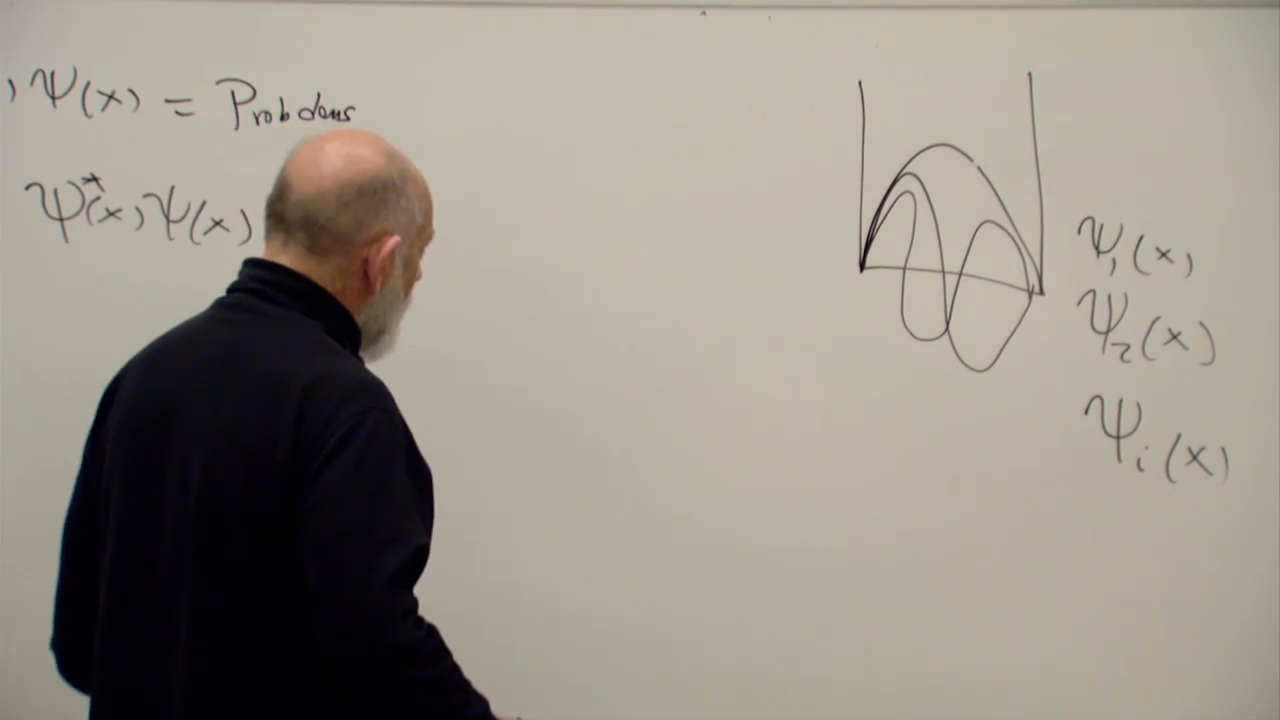
\includegraphics[width=0.94\linewidth]{lecture_07_frame_01.png}
\caption{Die Kastenmoden an der Vorlesungstafel. Links sind noch die Bornsche Einteilchen-Wahrscheinlichkeitsdichte und die Normierung zu sehen; der Potentialtopf rechts zeigt \(\psi_1(x)\), \(\psi_2(x)\) und die allgemeine Bezeichnung \(\psi_i(x)\).}
\lectureframe{00:08:25}
\end{figure}

Dieselbe Modenstruktur lässt sich auch unabhängig von der Überdeckung durch die Live-Tafel darstellen:
\begin{figure}[htbp]
\centering
\begin{tikzpicture}[x=1cm,y=1cm]
  \draw[thick] (0,0) -- (0,4.0);
  \draw[thick] (7,0) -- (7,4.0);
  \draw[gray!55] (0,2.85) -- (7,2.85);
  \draw[gray!55] (0,1.35) -- (7,1.35);
  \draw[blue!75!black,thick,domain=0:7,samples=120]
    plot (\x,{2.85+0.62*sin(180*\x/7)});
  \draw[teal!70!black,thick,domain=0:7,samples=120]
    plot (\x,{1.35+0.55*sin(360*\x/7)});
  \node[right] at (7.15,3.20) {$\psi_1(x)$};
  \node[right] at (7.15,1.70) {$\psi_2(x)$};
  \node at (3.5,0.38) {$\vdots\quad\psi_i(x)$};
\end{tikzpicture}
\caption{Eine saubere Rekonstruktion der qualitativen Kastenskizze. Die vertikalen Verschiebungen dienen lediglich dazu, die beiden Wellenfunktionen in der Darstellung voneinander zu trennen.}
\end{figure}

Die Orthonormalitätsbedingung lautet
\begin{equation}
\int dx\,\psi_i^*(x)\psi_j(x)=\delta_{ij}.
\label{eq:l07-orthonormality}
\end{equation}
Für \(i=j\) ist der Zustand normiert und das Integral gleich eins. Für \(i\ne j\) sind die beiden Zustände orthogonal und das Integral verschwindet.

Vollständigkeit ist die ebenso wichtige Aussage
\begin{equation}
\sum_i |i\rangle\langle i|=\mathbf 1.
\label{eq:l07-resolution}
\end{equation}
Jedes \(|i\rangle\langle i|\) projiziert auf eine Basisrichtung; die Summe über die vollständige Basis ist die Einheitsabbildung. Auf einen beliebigen Vektor angewandt, zerlegt sie ihn lediglich in seine Komponenten und setzt ihn wieder zusammen.

Nun schieben wir Gleichung~\eqref{eq:l07-resolution} zwischen zwei Ortszustände:
\begin{align}
\langle y|x\rangle
&=\sum_i\langle y|i\rangle\langle i|x\rangle \\
&=\sum_i\psi_i(y)\psi_i^*(x) \\
&=\delta(y-x).
\label{eq:l07-position-completeness}
\end{align}
Der Stern gehört an den Faktor, dessen Bra-Ket-Reihenfolge \(\langle i|x\rangle\) lautet. Vertauscht man \(x\) und \(y\), erhält man die komplex konjugierte, aber gleichwertige Form. Jede vollständige Orthonormalbasis liefert somit eine Darstellung der Deltafunktion. Sinus- und Kosinusfunktionen, Oszillator-Wellenfunktionen und Energie-Eigenfunktionen erfüllen alle dieselbe Aufgabe.

\begin{classroomqa}
\lecturetimestamp{00:13:43}
\audiencequestion{Muss die zweite Wellenfunktion in der Vollständigkeitssumme komplex konjugiert werden?}
\lecturerresponse{Ja. Bei der Reihenfolge \(\langle y|i\rangle\langle i|x\rangle\) lauten die Faktoren \(\psi_i(y)\psi_i^*(x)\). Wenn man die Bra-Ket-Reihenfolge sichtbar lässt, muss man nicht raten, wo der Stern hingehört.}
\end{classroomqa}

Das ist die Einteilchen-Mathematik, die wir benötigen. Nun wechseln wir den Zustandsraum.

\section{Der Fockraum als erweiterter Zustandsraum}

Für viele identische Teilchen ist eine Basis praktisch, die angibt, wie viele Teilchen jede Einteilchenmode besetzen:
\begin{equation}
|n_1,n_2,n_3,\ldots\rangle.
\label{eq:l07-fock-basis}
\end{equation}
Die ganze Zahl \(n_i\) ist die Besetzungszahl der Mode \(i\). Dieser Ket ist kein Einteilchenzustand in ausgefallener Schreibweise. Er gehört zu einem größeren Hilbertraum, der den Nullteilchensektor, sämtliche Einteilchenzustände, sämtliche Zweiteilchenzustände und so weiter enthält. Dieser größere Raum heißt Fockraum.

Um Besetzungen zu ändern, führen wir für jede Mode einen Erzeugungsoperator und einen Vernichtungsoperator ein:
\begin{equation}
a_i^\dagger,\qquad a_i.
\end{equation}
Der erste fügt der Mode \(i\) ein Teilchen hinzu, der zweite entfernt eines. Die Sprache des harmonischen Oszillators dient hier zunächst als Buchführungshilfe: Es muss keine tatsächliche Feder schwingen. Die Oszillatoralgebra liefert genau die Werkzeuge, die wir benötigen, um Besetzungszahlen zu erhöhen und zu verringern.

Der Besetzungszahloperator der Mode ist
\begin{equation}
\begin{aligned}
N_i&=a_i^\dagger a_i,\\
N_i|n_1,\ldots,n_i,\ldots\rangle
&=n_i|n_1,\ldots,n_i,\ldots\rangle.
\end{aligned}
\end{equation}
Das Vakuum ist
\begin{equation}
|0\rangle\equiv|0,0,0,\ldots\rangle,
\qquad
a_i|0\rangle=0
\quad\text{for every }i.
\label{eq:l07-vacuum}
\end{equation}
Ein Einteilchenzustand in der Mode \(i\) ist daher
\begin{equation}
|i\rangle=a_i^\dagger|0\rangle.
\label{eq:l07-mode-created}
\end{equation}
Dasselbe Symbol \(|i\rangle\) kann nun entweder als Einteilchenbasisvektor oder als dieser Vektor aufgefasst werden, eingebettet in den Einteilchensektor des Fockraums. Die Einbettung ist Gleichung~\eqref{eq:l07-mode-created}; aus dem jeweiligen Kontext geht hervor, welcher Raum gemeint ist.

\section{Die Moden zu einem Feld zusammenfassen}

Wir definieren das Vernichtungsfeld und das Erzeugungsfeld durch
\begin{equation}
\Psi(x)=\sum_i \psi_i(x)a_i,
\qquad
\Psi^\dagger(x)=\sum_i \psi_i^*(x)a_i^\dagger.
\label{eq:l07-field-expansion}
\end{equation}
Die Großschreibung ist wichtig. Die kleingeschriebenen Funktionen \(\psi_i(x)\) sind komplexe Zahlen; das großgeschriebene \(\Psi(x)\) ist ein Operator auf dem Fockraum. Für jeden Raumpunkt \(x\) ergibt Gleichung~\eqref{eq:l07-field-expansion} eine andere Linearkombination der Modenoperatoren. Das bedeutet es, wenn man von einer operatorwertigen Funktion des Ortes spricht.

Bei freien Teilchen können die Modenfunktionen ebene Wellen \(e^{ikx}\) sein. Dann ist Gleichung~\eqref{eq:l07-field-expansion} eine Fourierentwicklung, nur dass ihre Fourierkoeffizienten Operatoren statt Zahlen sind. In der älteren Terminologie heißen gewöhnliche komplexe Zahlen \(c\)-Zahlen und Quantenoperatoren \(q\)-Zahlen. Die Modenfunktionen sind \(c\)-Zahlen und kommutieren mit allem; \(a_i\) und \(a_i^\dagger\) tragen den Operatorcharakter.

Weder \(\Psi\) noch \(\Psi^\dagger\) ist hermitesch. Ihre adjungierten Operatoren sind jeweils der andere. Die beiden Kombinationen
\begin{equation}
\Psi+\Psi^\dagger,
\qquad
i(\Psi^\dagger-\Psi)
\label{eq:l07-hermitian-combinations}
\end{equation}
sind hermitesch und können Observablen darstellen. Vorerst sind die Felder jedoch vor allem nützlich, um Teilchen lokal zu erzeugen, zu vernichten und zu zählen.

\begin{classroomqa}
\lecturetimestamp{00:21:05}
\audiencequestion{Was bedeutet es, dass ein Operator von \(x\) abhängt?}
\lecturerresponse{Das bedeutet, dass jeder Wert von \(x\) einen anderen Operator auswählt. Die Ortsabhängigkeit steckt in den gewöhnlichen Modenfunktionen, während jede daraus entstehende Linearkombination auf denselben Fockraum wirkt.}
\end{classroomqa}

\section{Was das Erzeugungsfeld bewirkt}

Eine Definition wird nützlich, wenn wir fragen, was sie bewirkt. Wir beginnen mit einem Orts-Eigenzustand im Einteilchensektor und setzen die Vollständigkeitsrelation ein:
\begin{align}
|x\rangle
&=\sum_i |i\rangle\langle i|x\rangle \\
&=\sum_i a_i^\dagger|0\rangle\,\psi_i^*(x) \\
&=\Psi^\dagger(x)|0\rangle.
\label{eq:l07-local-creation}
\end{align}
Damit erzeugt \(a_i^\dagger\) ein Teilchen in der genau festgelegten Mode \(i\), während \(\Psi^\dagger(x)\) ein bei \(x\) lokalisiertes Teilchen erzeugt. In der idealisierten Ortsbasis ist diese Lokalisierung distributionell; bei einer physikalischen Präparation würde man ein schmales Wellenpaket verwenden, doch die algebraische Bedeutung ist dieselbe.

\begin{classroomqa}
\lecturetimestamp{00:24:48}
\audiencequestion{Ist \(\sum_i|i\rangle\langle i|\) eine Projektion?}
\lecturerresponse{Jeder Summand ist eine Projektion auf einen Basiszustand. Die vollständige Summe ist die Einheitsabbildung selbst und heißt Vollständigkeitsrelation. Ihr Einsetzen ändert den Zustand nicht, macht aber seine Komponenten bezüglich der gewählten Basis sichtbar.}
\end{classroomqa}

Gleichung~\eqref{eq:l07-local-creation} liefert die erste direkte Teilcheninterpretation des Feldes. Wir haben einem abstrakten Operator nicht bloß eine Ortsangabe hinzugefügt. Wir haben die Operation konstruiert, die ein Teilchen an diesem Ort erzeugt.

\begin{classroomqa}
\lecturetimestamp{00:28:20}
\audiencequestion{Sollte das Erzeugungsfeld im Ortsraum mit einem Stern oder einem Dolch gekennzeichnet werden?}
\lecturerresponse{Für das Adjungieren eines Operators verwendet man einen Dolch. Sterne bezeichnen die komplexe Konjugation der gewöhnlichen Wellenfunktionen \(\psi_i(x)\); Dolche gehören an \(a_i^\dagger\) und \(\Psi^\dagger(x)\).}
\end{classroomqa}

\begin{classroomqa}
\lecturetimestamp{00:28:36}
\audiencequestion{Darf man die Erzeugungsoperatoren in der Modenentwicklung an den Wellenfunktionen vorbeiziehen?}
\lecturerresponse{Ja. Die \(\psi_i(x)\) sind \(c\)-Zahlen und kommutieren daher mit jedem Operator. Vorsicht ist nur geboten, wenn man die Reihenfolge nicht kommutierender Operatoren wie \(a_i\) und \(a_j^\dagger\) ändert.}
\end{classroomqa}

\section{Von der Wahrscheinlichkeitsdichte zur Teilchendichte}

Spielen wir nun ein wenig mit dem Feld. Der naheliegendste erste Ausdruck ist
\begin{equation}
\int dx\,\Psi^\dagger(x)\Psi(x).
\end{equation}
Er sieht aus wie das Normierungsintegral für ein Teilchen, doch seine Faktoren sind jetzt Operatoren. Setzen wir die Modenentwicklungen ein, ohne ihre Reihenfolge zu ändern:
\begin{align}
\int dx\,\Psi^\dagger(x)\Psi(x)
&=\int dx
\left(\sum_i a_i^\dagger\psi_i^*(x)\right)\\
&\qquad\times\left(\sum_j a_j\psi_j(x)\right) \\
&=\sum_{i,j}a_i^\dagger a_j
\int dx\,\psi_i^*(x)\psi_j(x) \\
&=\sum_{i,j}a_i^\dagger a_j\,\delta_{ij} \\
&=\sum_i a_i^\dagger a_i.
\label{eq:l07-number-derivation}
\end{align}
Damit lautet der Gesamtteilchenzahloperator
\begin{equation}
N=\sum_i N_i
=\int dx\,\Psi^\dagger(x)\Psi(x).
\label{eq:l07-total-number}
\end{equation}
Bei den hier betrachteten Zuständen nehmen die Besetzungszahlen von Anregungen endlicher Energie bei hinreichend hoher Modenenergie ab. Daher ist diese Gesamtzahl gewöhnlich endlich, obwohl es unendlich viele mögliche Moden gibt.

Der Integrand ist der lokale Teilchendichteoperator:
\begin{equation}
n(x)=\Psi^\dagger(x)\Psi(x).
\label{eq:l07-density}
\end{equation}
Genau genommen misst man die Dichte nicht an einem mathematischen Punkt. Für ein kleines Gebiet \(R\) misst man
\begin{equation}
N_R=\int_R dx\,n(x),
\label{eq:l07-regional-number}
\end{equation}
die Zahl der Teilchen in diesem Gebiet. Wie jede Quantenobservable muss \(N_R\) in einem beliebigen Zustand keinen bestimmten Wert haben. Bei wiederholten Präparationen können unterschiedliche Messergebnisse auftreten.

\begin{classroomqa}
\lecturetimestamp{00:36:27}
\audiencequestion{Ist \(\Psi^\dagger(x)\Psi(x)\) die Wahrscheinlichkeitsdichte für mehrere Teilchen?}
\lecturerresponse{Ihre unmittelbare Bedeutung ist die Teilchendichte. Eine Vielteilchen-Wahrscheinlichkeitsamplitude hängt im Allgemeinen von allen Teilchenkoordinaten ab. Die lokale bilineare Größe zählt dagegen Teilchen in einem kleinen Gebiet, wenn man sie über dieses Gebiet integriert.}
\end{classroomqa}

\begin{classroomqa}
\lecturetimestamp{00:38:28}
\audiencequestion{Wirken die Operatoren \(a_i\) und \(a_i^\dagger\) nur auf Zustandsvektoren und nicht auf die Einteilchen-Wellenfunktionen?}
\lecturerresponse{Ja. Sie wirken auf Zustände im Fockraum, etwa \(|n_1,n_2,\ldots\rangle\). Die Einteilchen-Modenfunktionen, die sie multiplizieren, sind gewöhnliche Zahlen und nicht die Objekte, auf die diese Leiteroperatoren wirken.}
\end{classroomqa}

Die Besetzungskets bilden eine Basis, sind aber nicht der allgemeinste Zustand. Man kann sie überlagern, auch so, dass dieselbe Gesamtteilchenzahl auf unterschiedliche Weise auf die Moden verteilt ist. Bei neutralen Teilchensorten wie Photonen kann man außerdem Zustände mit unterschiedlicher Gesamtteilchenzahl überlagern. Der Operator in Gleichung~\eqref{eq:l07-regional-number} hat in allen solchen Zuständen dieselbe operationale Bedeutung.

\begin{classroomqa}
\lecturetimestamp{00:40:01}
\audiencequestion{Wird die Teilchendichte, wenn man sie durch die Gesamtteilchenzahl teilt, zur Wahrscheinlichkeitsdichte, ein Teilchen bei \(x\) zu finden?}
\lecturerresponse{Bei festem \(N\) und großer Teilchenzahl ist \(N_R/N\) eine relative Häufigkeit und entspricht meist sehr gut einer Einteilchen-Wahrscheinlichkeit. Es handelt sich jedoch nicht um eine Operatoridentität, die ein einzelnes Messergebnis mit einer Wahrscheinlichkeit gleichsetzt. Die gemessene Teilchenzahl schwankt; in einem Bild unabhängiger Teilchen typischerweise um einen Betrag der Größenordnung \(\sqrt N\). Ein außergewöhnlicher Messlauf kann stark von der Wahrscheinlichkeit abweichen, auch wenn ein solcher Lauf unwahrscheinlich ist.}
\end{classroomqa}

\begin{classroomqa}
\lecturetimestamp{00:42:25}
\audiencequestion{Was geschieht mit der Ladungserhaltung bei einer Überlagerung eines Ein-Elektron-Zustands mit einem Zustand ohne Elektronen?}
\lecturerresponse{Das ist nicht die Art von Überlagerung, die man in einem abgeschlossenen Sektor mit fester elektrischer Ladung verwendet. Überlagern kann man verschiedene Verteilungen mit derselben Gesamtladung. Photonen tragen keine elektrische Ladung, daher entsteht bei verschiedenen Photonenzahlsektoren kein solches Problem. Auch die Elektronen- und Positronenzahl kann sich gemeinsam ändern, während die Nettoladung erhalten bleibt.}
\end{classroomqa}

\section{Die Energie unabhängiger Teilchen}

Die nächste Observable ist die Energie. Betrachten wir zunächst Teilchen, die nicht miteinander wechselwirken. Für ein verdünntes System ist das oft eine gute Näherung. Auch Photonen wechselwirken prinzipiell über Prozesse höherer Ordnung, doch gewöhnliche Laborstrahlung ist hinreichend verdünnt, sodass die Beschreibung durch unabhängige Teilchen ausgezeichnet funktioniert.

Sei \(\omega_i\) die Energie eines Teilchens in der Mode \(i\), wobei \(\hbar=1\) gilt. Eine Mode bezeichnet einen Einteilchenzustand. Der Gesamt-Hamiltonoperator lautet dann
\begin{equation}
H=\sum_i\omega_i N_i
=\sum_i\omega_i a_i^\dagger a_i.
\label{eq:l07-mode-hamiltonian}
\end{equation}
Jede besetzte Mode trägt für jedes Teilchen einmal ihre Einteilchenenergie bei.

\begin{classroomqa}
\lecturetimestamp{00:48:16}
\audiencequestion{Ist \(\omega_i\) eine Funktion des Ortes?}
\lecturerresponse{Nein. Es ist der Energie-Eigenwert der Mode \(i\). Die Funktion \(\psi_i(x)\) hängt vom Ort ab; \(\omega_i\) hängt davon ab, welches Energieniveau ausgewählt wurde.}
\end{classroomqa}

Die Werte \(\omega_i\) sind durch die zeitunabhängige Einteilchen-Schrödinger-Gleichung bestimmt. Wir definieren
\begin{equation}
h=-\frac{\nabla^2}{2m}+V(x).
\label{eq:l07-one-particle-h}
\end{equation}
Dann gilt
\begin{equation}
h\psi_i(x)=\omega_i\psi_i(x).
\label{eq:l07-schrodinger-eigenvalue}
\end{equation}
In einer Dimension ist der Impulsoperator \(p=-i\partial_x\), und \(p^2/(2m)\) wird zu \(-\partial_x^2/(2m)\). In drei Dimensionen fassen sich die drei zweiten Ableitungen zu \(-\nabla^2/(2m)\) zusammen.

\begin{figure}[htbp]
\centering
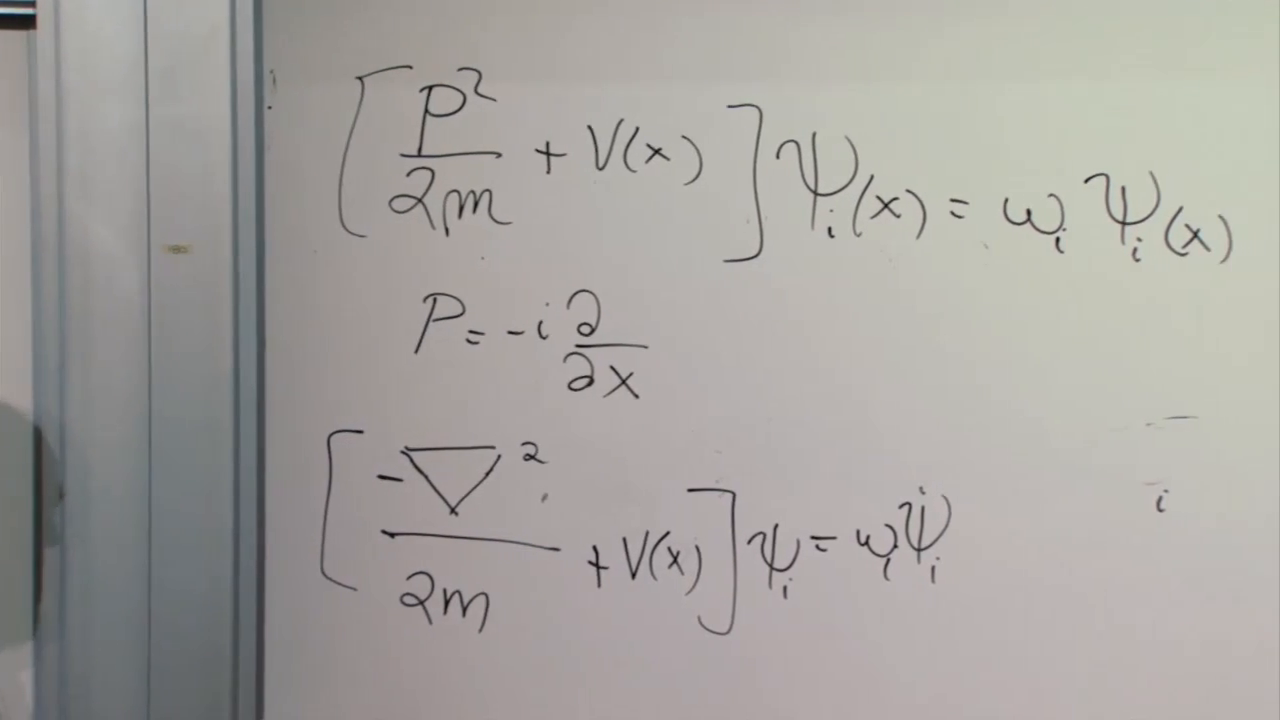
\includegraphics[width=0.94\linewidth]{lecture_07_frame_02.png}
\caption{Der Tafelabschnitt vom Ausdruck \(p^2/(2m)+V(x)\) bis zur Differentialform der Einteilchen-Schrödinger-Eigenwertgleichung. Gleichung~\eqref{eq:l07-schrodinger-eigenvalue} ist ihre bereinigte Rekonstruktion.}
\lectureframe{00:54:10}
\end{figure}

Für eine beliebige normierte Einteilchen-Wellenfunktion lautet der bekannte Erwartungswert
\begin{equation}
\langle h\rangle_\psi
=\int dx\,\psi^*(x)h\psi(x).
\label{eq:l07-one-particle-energy-expectation}
\end{equation}
Die Vielteilchenformel liegt nahe, wenn man die kleingeschriebene Wellenfunktion durch das operatorwertige Feld ersetzt. Das ist noch kein Beweis, sondern die Vermutung, deren Richtigkeit wir jetzt prüfen:
\begin{equation}
H=\int dx\,\Psi^\dagger(x)h\Psi(x).
\label{eq:l07-field-hamiltonian}
\end{equation}

\section{Zuerst die Antwort hinschreiben, dann beweisen}

Setzen wir Gleichung~\eqref{eq:l07-field-expansion} in den vorgeschlagenen Hamiltonoperator ein:
\begin{align}
\int dx\,\Psi^\dagger h\Psi
&=\int dx
\left(\sum_i a_i^\dagger\psi_i^*(x)\right)
h\left(\sum_j a_j\psi_j(x)\right) \\
&=\sum_{i,j}a_i^\dagger a_j
\int dx\,\psi_i^*(x)h\psi_j(x).
\label{eq:l07-h-expanded}
\end{align}
Der Differentialoperator \(h\) wirkt auf die von \(x\) abhängige Wellenfunktion \(\psi_j(x)\), nicht auf den Modenoperator \(a_j\). Nach der Schrödinger-Gleichung gilt
\begin{equation}
h\psi_j(x)=\omega_j\psi_j(x).
\end{equation}
Folglich
\begin{align}
\int dx\,\Psi^\dagger h\Psi
&=\sum_{i,j}a_i^\dagger a_j\omega_j
\int dx\,\psi_i^*(x)\psi_j(x) \\
&=\sum_{i,j}a_i^\dagger a_j\omega_j\delta_{ij} \\
&=\sum_j\omega_j a_j^\dagger a_j.
\label{eq:l07-h-proof}
\end{align}
Das ist genau Gleichung~\eqref{eq:l07-mode-hamiltonian}. Der lokale Feldausdruck und die Summe aller Teilchenenergien sind derselbe Operator.

\begin{figure}[htbp]
\centering
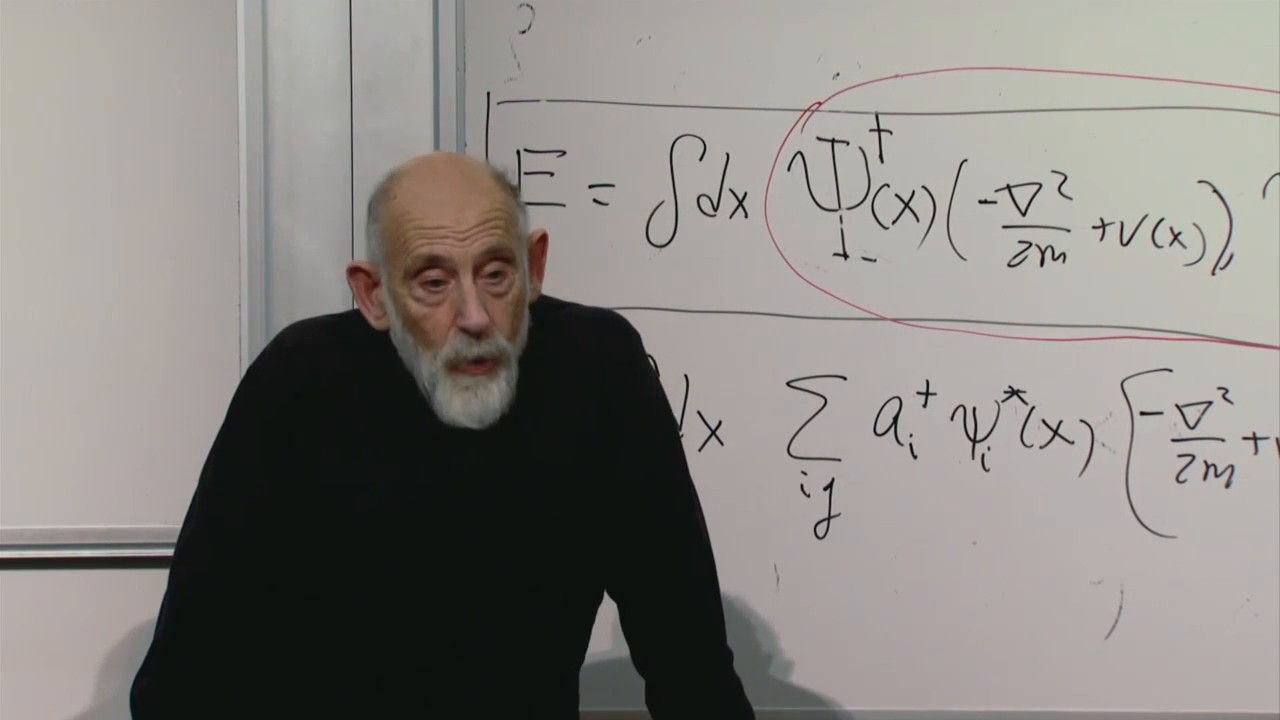
\includegraphics[width=0.94\linewidth]{lecture_07_frame_03.png}
\caption{Der an der Tafel hervorgehobene Feld-Hamiltonoperator; darunter beginnt der Beweis mit der Modenentwicklung. Der Live-Ausschnitt bleibt als Beleg erhalten; Gleichungen~\eqref{eq:l07-field-hamiltonian}--\eqref{eq:l07-h-proof} stellen die vollständige Rechnung wieder her.}
\lectureframe{01:05:34}
\end{figure}

Bei dieser Herleitung wurde kein Erzeugungsoperator an einem Vernichtungsoperator vorbeikommutiert. Die Reihenfolge \(a_i^\dagger a_j\) bleibt vom Anfang bis zum Ende erhalten. Nur die Wellenfunktionen und Eigenwerte, also \(c\)-Zahlen, werden frei verschoben.

\section{Warum ist das ein Feld?}

Warum nennen wir \(\Psi(x)\) ein Feld? Weil es eine operatorwertige Größe ist, die an jedem Raumpunkt definiert ist, und weil daraus gebildete hermitesche Kombinationen oder bilineare Ausdrücke lokale Observablen sind. Die Dichte \(n(x)\) und der weiter unten angegebene lokale Energieausdruck sind zwei Beispiele. Hinter dem Wort verbirgt sich kein zusätzliches mathematisches Kriterium.

Dieses Feld ist nicht das elektromagnetische Feld. Es beschreibt die nichtrelativistische Teilchensorte, deren Einteilchenmoden und Hamiltonoperator \(p^2/(2m)+V\) zugrunde gelegt wurden: beispielsweise langsam bewegte Atome, Neutronen, Protonen oder Elektronen. Diese Teilchen sind die Quanten des jeweils zugehörigen Feldes, in demselben strukturellen Sinn, in dem Photonen die Quanten des elektromagnetischen Feldes sind.

\begin{classroomqa}
\lecturetimestamp{01:02:45}
\audiencequestion{Wo ist beim Übergang vom Vielteilchensystem zur obigen Formel ein Feld ins Spiel gekommen?}
\lecturerresponse{In Gleichung~\eqref{eq:l07-field-expansion}: \(\Psi(x)\) ist ein Operator an jedem Raumpunkt. Die anschließenden Herleitungen zeigen, dass seine lokalen Produkte Teilchen- und Energiedichten messen. Ortsabhängigkeit zusammen mit Operatorcharakter ist genau die Feldstruktur, die wir konstruieren.}
\end{classroomqa}

\section{Lokale Energiedichte}

Gleichung~\eqref{eq:l07-field-hamiltonian} schreibt die Gesamtenergie als Integral über den Raum:
\begin{equation}
\begin{aligned}
H&=\int dx\,\mathcal H(x),\\
\mathcal H(x)
&=-\frac{1}{2m}\Psi^\dagger(x)\nabla^2\Psi(x)\\
&\quad+V(x)\Psi^\dagger(x)\Psi(x).
\end{aligned}
\label{eq:l07-hamiltonian-density}
\end{equation}
Der Integrand ist eine naheliegende lokale Energiedichte für diesen Hamiltonoperator. Ihre lokale Form ist nicht eindeutig. So ersetzt die partielle Integration den kinetischen Term durch
\begin{equation}
\mathcal H_{\rm kin}(x)
=\frac{1}{2m}\nabla\Psi^\dagger(x)\mathbin{\cdot}\nabla\Psi(x)
\label{eq:l07-kinetic-density}
\end{equation}
bis auf einen Randterm. Unter den üblichen Randbedingungen ergeben beide Ausdrücke denselben Gesamt-Hamiltonoperator. Das ist die kleine Mehrdeutigkeit, die in der Vorlesung erwähnt wurde.

\begin{classroomqa}
\lecturetimestamp{01:05:57}
\audiencequestion{Muss man die Energiedichte über den gesamten Raum integrieren?}
\lecturerresponse{Die Integration über den gesamten Raum ergibt die Gesamtenergie. Die Integration über ein kleineres Gebiet ergibt die diesem Gebiet zugeordnete Energie, wobei die gewöhnliche Mehrdeutigkeit bei der Wahl einer lokalen Dichte zu berücksichtigen ist, deren Integral über den ganzen Raum denselben Hamiltonoperator ergibt.}
\end{classroomqa}

\begin{classroomqa}
\lecturetimestamp{01:06:25}
\audiencequestion{Wie unterscheidet sich das großgeschriebene \(N_i\) in der Energieformel vom kleingeschriebenen \(n_i\)?}
\lecturerresponse{\(N_i=a_i^\dagger a_i\) ist ein Operator. Die ganze Zahl \(n_i\) ist einer seiner Eigenwerte auf einem Besetzungszahlzustand. Operatoren wirken auf Zustände; ihre Eigenwerte sind gewöhnliche Zahlen.}
\end{classroomqa}

\begin{classroomqa}
\lecturetimestamp{01:06:46}
\audiencequestion{Kann man den Feld-Hamiltonoperator selbst in Dirac-Notation als Bra oder Ket schreiben?}
\lecturerresponse{Nein. Bras und Kets bezeichnen Zustandsvektoren und ihre Dualvektoren. Das Feld und der Hamiltonoperator sind Operatoren, die auf diese Zustände wirken. Ein Erwartungswert wie \(\langle\Phi|H|\Phi\rangle\) verwendet beide Arten von Objekten; man darf sie nicht gleichsetzen.}
\end{classroomqa}

\section{Ein Teilchen zurückgewinnen und sich einem klassischen Feld nähern}

Der erweiterte Formalismus enthält die gewöhnliche Einteilchen-Quantenmechanik. Beschränken wir den Fockraum auf Zustände, für die
\begin{equation}
N|\Phi\rangle=|\Phi\rangle.
\end{equation}
gilt. Innerhalb dieses Sektors reproduziert die Feldkonstruktion jeden Einteilchenzustand und jede Einteilchenvorhersage. Wir haben die alte Theorie nicht ersetzt, sondern sie in einen Raum eingebettet, der auch null, zwei oder beliebig viele Teilchen beschreiben kann.

Am anderen Ende kann sich eine Mode, die von sehr vielen Bosonen besetzt ist, näherungsweise wie eine klassische Welle verhalten. In geeigneten kohärenten oder semiklassischen Zuständen erfüllt der Erwartungswert
\begin{equation}
\Phi_{\rm cl}(x,t)=\langle\Psi(x,t)\rangle
\end{equation}
die klassisch anmutende Gleichung
\begin{equation}
i\partial_t\Phi_{\rm cl}(x,t)
=\left(-\frac{\nabla^2}{2m}+V(x)\right)\Phi_{\rm cl}(x,t)
\label{eq:l07-classical-schrodinger}
\end{equation}
für die freie nichtrelativistische Theorie. Die Vorlesung stellt diesen Zusammenhang dar, ohne ihn herzuleiten. Er bildet die Brücke zwischen einer Ansammlung von Quanten und einem Wellenfeld: Bei großer Besetzung werden die relativen Fluktuationen klein, sodass sich geeignete Erwartungswerte klassisch verhalten.

Der Formalismus ist also zugleich Buchführung und Physik. Er ordnet alle Teilchenzahlsektoren, erfasst aber auch Interferenz, Verschränkung und das Entstehen klassischer Wellen aus Quantenteilchen.

\begin{classroomqa}
\lecturetimestamp{01:10:43}
\audiencequestion{Warum lassen sich die Erzeugungs- und Vernichtungsoperatoren im Integral beinahe wie gewöhnliche Zahlen behandeln?}
\lecturerresponse{Sie wurden nie miteinander vertauscht. Die gewöhnlichen Modenfunktionen kommutieren mit ihnen, und die Ableitungen wirken nur auf diese Funktionen. Einen Vernichtungsoperator an einem Erzeugungsoperator vorbeizuziehen, würde den Kommutator erfordern und könnte einen zusätzlichen Term ergeben; in der Herleitung wird dieser Schritt nicht ausgeführt.}
\end{classroomqa}

\section{Ein Einschub zur Dirac-Notation}

Ein Teil der Verwirrung ist historisch bedingt. Eine Einteilchen-Wellenfunktion erfüllt eine Wellengleichung und sieht oberflächlich wie ein klassisches Feld aus, ist zugleich aber eine Wahrscheinlichkeitsamplitude. Die frühe Quantentheorie musste diese Rollen auseinanderhalten und anschließend erklären, wie echte messbare Wellenfelder wie das elektromagnetische Feld aus Quanten aufgebaut sind. Fockraum und operatorwertige Felder lösen den scheinbaren Widerspruch auf.

Die Dirac-Notation fasst diese Unterscheidung besonders knapp. Ein Ket gehört zu einem Vektorraum, ein Bra zu seinem Dualraum, und ihre Nebeneinanderschreibung bildet ein Skalarprodukt. Die Vollständigkeitsrelation
\begin{equation}
\sum_i|i\rangle\langle i|=\mathbf 1
\end{equation}
wird damit beinahe selbsterklärend. Die Vorlesung veranschaulicht dies anhand einer Anekdote aus dem Quantenmechanikunterricht für Mathematiker: Der mathematische Inhalt war bereits vertraut, doch die Notation machte routinemäßige Umformungen so durchsichtig, dass die Struktur neu erschien. Es geht nicht darum, dass einer Fachrichtung der Begriff fehlte. Eine gut gewählte Notation kann vielmehr dafür sorgen, dass die zulässigen Operationen kaum zu verwechseln sind.

Das ist hier wichtig. Es gibt nun mehrere verschiedene Operatoren:
\begin{itemize}
\item \(h\) wirkt als Differentialoperator auf Einteilchen-Wellenfunktionen;
\item \(a_i\) und \(a_i^\dagger\) wirken auf Besetzungszahlzustände im Fockraum;
\item \(\Psi(x)\), \(\Psi^\dagger(x)\), \(N\) und \(H\) wirken ebenfalls auf den Fockraum.
\end{itemize}
Die Entwicklung in Gleichung~\eqref{eq:l07-field-expansion} verknüpft die ersten beiden Bereiche, ohne sie miteinander zu verschmelzen.

\begin{classroomqa}
\lecturetimestamp{01:18:16}
\audiencequestion{Sind Felder nur ein Formalismus zur Beschreibung von Teilchensammlungen?}
\lecturerresponse{Sie sind ein Formalismus, aber kein inhaltsleerer. Ihre lokalen Observablen lassen sich messen, und die Teilchen sind Quantenobjekte mit Interferenz und Verschränkung, keine klassischen Kügelchen. Die Feldoperatoren kodieren genau diese messbaren kollektiven Eigenschaften.}
\end{classroomqa}

\section{Relativistische Vorsicht und ein Exkurs zum Elektromagnetismus}

Die bisherige Konstruktion ist nichtrelativistisch. Der Impuls bleibt in der relativistischen Physik eine gute Teilchenbezeichnung, doch die scharfe Lokalisierung eines Teilchens am Ort ist wesentlich problematischer. Daher ist eine lokale Photonenzahldichte im Allgemeinen kein so klar definierter Gegenstand wie die nichtrelativistische Dichte \(n(x)\). Die Energiedichte bleibt wohldefiniert und ist die sicherere lokale Observable.

Die Vorlesung führt eine nützliche, ausdrücklich heuristische Analogie zum Elektromagnetismus an. Man fasse das elektrische und das magnetische Feld zum komplexen Vektor
\begin{equation}
\mathbf F=\mathbf E+i\mathbf B,
\qquad
\mathbf F^*=\mathbf E-i\mathbf B.
\label{eq:l07-riemann-silberstein}
\end{equation}
zusammen. Dann gilt
\begin{equation}
\mathbf F^*\mathbin{\cdot}\mathbf F
=\mathbf E^2+\mathbf B^2,
\label{eq:l07-em-density}
\end{equation}
was in konventionellen Einheiten proportional zur elektromagnetischen Energiedichte ist. Das ist nicht wörtlich eine Photon-Wahrscheinlichkeitsdichte. Treffender ist es, diese Größe als kompakte Feldvariable zu verstehen, deren Betragsquadrat die Energiedichte misst, oder informell als Photonendichte, gewichtet mit der Photonenenergie.

\begin{classroomqa}
\lecturetimestamp{01:19:10}
\audiencequestion{Kann man die Photonendichte mit der Stärke des elektrischen Feldes gleichsetzen?}
\lecturerresponse{Nur qualitativ und mit Vorsicht. Für relativistische Photonen ist die lokale Teilchenzahl nicht der bevorzugte Begriff. Die belastbare Aussage ist, dass \(E^2+B^2\) proportional zur Energiedichte ist und dass die komplexe Kombination \(\mathbf E+i\mathbf B\) die Maxwell-Gleichungen in einer Schrödinger-ähnlichen Form zusammenfasst.}
\end{classroomqa}

\begin{classroomqa}
\lecturetimestamp{01:20:09}
\audiencequestion{Warum kann ein relativistisches Teilchen einen bestimmten Impuls haben, während sein Ort problematisch ist?}
\lecturerresponse{Der Impuls kennzeichnet relativistische Einteilchen-Darstellungen eindeutig, wohingegen eine strikte Lokalisierung mit der Teilchenerzeugung und der relativistischen Feldbeschreibung in Konflikt gerät. Diese Vorlesung entwickelt jene Theorie nicht; der Hinweis markiert die Grenze der hier behandelten nichtrelativistischen Deutung der Dichte.}
\end{classroomqa}

\section{Operatorordnung und die Grundzustandskonstante}

Die Operatorreihenfolge darf nicht leichtfertig geändert werden. Für bosonische Moden gilt
\begin{equation}
a_i a_i^\dagger=a_i^\dagger a_i+1.
\end{equation}
Ersetzt man daher die Normalordnung \(\Psi^\dagger h\Psi\) durch die umgekehrte Reihenfolge \((h\Psi)\Psi^\dagger\) oder die entsprechende integrierte Form, kommt der Kommutatorbeitrag hinzu. In einer Modenbasis ist dies eine additive Summe von einer Energiequant pro Mode. Es handelt sich um die Grundzustands- oder Nullpunktskonstante, die im Kontinuum regularisiert werden muss. Die Vorlesung geht diesem Problem hier nicht weiter nach; sie weist lediglich darauf hin, dass die beiden Anordnungen nicht gleich sind.

\begin{classroomqa}
\lecturetimestamp{01:22:04}
\audiencequestion{Was geschieht, wenn \(\Psi\) und \(\Psi^\dagger\) im Hamiltonoperator vertauscht werden?}
\lecturerresponse{Ihr Kommutator muss berücksichtigt werden. Beim Umkehren der Reihenfolge kommt daher ein zustandsunabhängiger Grundzustandsbeitrag hinzu, statt dass derselbe Ausdruck entsteht. Der angegebene Hamiltonoperator steht in Normalordnung, \(\Psi^\dagger h\Psi\).}
\end{classroomqa}

\section{Der Impuls als letzter Test}

In den letzten Minuten wird dieselbe Ersetzung noch einmal vorgenommen. Für ein Teilchen gilt
\begin{equation}
\langle p\rangle_\psi
=\int dx\,\psi^*(x)\left(-i\partial_x\right)\psi(x).
\label{eq:l07-one-particle-momentum}
\end{equation}
Ersetzt man die Wellenfunktion durch das Feld, erhält man den Operator des Gesamtimpulses
\begin{equation}
P=\int dx\,\Psi^\dagger(x)\left(-i\partial_x\right)\Psi(x),
\label{eq:l07-field-momentum}
\end{equation}
oder in drei Dimensionen
\begin{equation}
\mathbf P=\int d^3x\,\Psi^\dagger(\mathbf x)
\left(-i\boldsymbol\nabla\right)\Psi(\mathbf x).
\end{equation}
Felder tragen Impuls. Ein hinreichend leistungsstarker Laser überträgt Impuls auf eine Wand und übt eine Kraft auf sie aus; in der quantenmechanischen Beschreibung ist dieser Feldimpuls die Summe der Impulse der Photonen.

Gleichung~\eqref{eq:l07-field-momentum} gibt einen Operator an, keinen Erwartungswert. Für einen Fock-Raum-Zustand \(|\Phi\rangle\) kann man dann berechnen
\begin{equation}
\langle P\rangle_\Phi=\langle\Phi|P|\Phi\rangle.
\end{equation}
Für die Bildung eines Erwartungswerts sind sowohl ein Operator als auch ein Zustand erforderlich. Wer die Observable mit ihrem Mittelwert verwechselt, verwischt genau den Unterschied, den diese Vorlesung herausgearbeitet hat.

\begin{classroomqa}
\lecturetimestamp{01:26:02}
\audiencequestion{Ist der angegebene Feldimpuls bereits der mittlere Impuls?}
\lecturerresponse{Nein. Er ist der hermitesche Operator, der die Observable darstellt. Gibt man einen Zustand vor, erhält man den Erwartungswert, indem man den Operator zwischen dessen Bra und Ket einfasst; bei einer Messung kann der Messwert weiterhin um diesen Mittelwert schwanken.}
\end{classroomqa}

Dies ist ein natürlicher Schlusspunkt. Ausgehend von Teilchen haben wir lokale Erzeugungs- und Vernichtungsfelder konstruiert, sie zum Zählen von Teilchen verwendet und die Summe der Einteilchenenergien und -impulse als Feldoperatoren umgeschrieben. Der nächste Schritt ist keine weitere Änderung der Schreibweise. Nun sollen Feldoperatoren physikalische Prozesse darstellen: Teilchen zerfallen, Teilchen streuen und Teilchensorten ineinander umgewandelt werden.
\chapter{Mischung, Oszillation, elektrische Dipolmomente und Feldoperatoren}

Wir beginnen etwas abseits des angekündigten Themas mit einer Frage zu Neutrinos. Es gibt Hinweise darauf, dass Neutrinos Masse haben und dass sich die Neutrinotypen mischen. Wenn die Massen nicht alle gleich sind, wie kann dann ein Typ in einen anderen übergehen, ohne die Energieerhaltung zu verletzen?

Die Frage führt zu einem Muster, das in der gesamten Quantenmechanik auftritt: Die Zustände, in denen ein System präpariert oder nachgewiesen wird, müssen nicht die Zustände sein, die seinen Hamiltonoperator diagonalisieren. Ein Zustand mit bestimmter Energie nimmt lediglich eine Phase auf. Ein präparierter Zustand, der eine Überlagerung mehrerer Energien ist, ändert sich, weil seine Komponenten unterschiedliche Phasen aufnehmen. Diese Unterscheidung führt uns vom Doppelmuldenpotential über Neutrinooszillationen bis zur Spinpräzession. Nach einem Exkurs zum elektrischen Dipolmoment des Elektrons kehren wir zur zweiten Quantisierung zurück und sehen dieselbe Orts--Impuls-Fourierstruktur auf der Ebene der Operatoren.

\section{Mischung als eigentliches Problem}

Neutrinos müssen nicht alle dieselbe Masse haben. Die Energieeigenzustände mischen sich nicht miteinander; jeder entwickelt sich unabhängig. Was wir den \emph{Typ} oder Flavor eines Neutrinos nennen, hängt damit zusammen, wie es erzeugt und nachgewiesen wird; ein Flavorzustand kann eine Linearkombination von Masse-Energie-Eigenzuständen sein. Schematisch gilt
\begin{equation}
|\text{type}\rangle = \sum_n c_n |E_n\rangle .
\end{equation}
Die richtige Aussage lautet also nicht, dass Energieeigenzustände ineinander übergehen, sondern dass die als ``Elektron-Neutrino'' oder ``Myon-Neutrino'' bezeichneten Zustände nicht selbst Energieeigenzustände sein müssen.

\begin{classroomqa}
\lecturetimestamp{00:00:09}
\audiencequestion{Wenn Neutrinos unterschiedliche Massen haben, wie können sie sich mischen, während die Energie erhalten bleibt?}
\lecturerresponse{Die Masse-Energie-Eigenzustände gehen nicht ineinander über. Elektron-, Myon- und Tau-Flavorzustände sind unterschiedliche Linearkombinationen dieser Eigenzustände. Jede Massenkomponente entwickelt sich mit ihrer eigenen Phase, und die Interferenz verändert die Flavorwahrscheinlichkeiten, ohne die Energieerhaltung zu verletzen.}
\end{classroomqa}

Für diese Struktur gibt es viele Beispiele. Das anschaulichste beginnt mit einem Teilchen in einem symmetrischen Doppelmuldenpotential.

\section{Symmetrisches Doppelmuldenpotential und näherungsweise lokalisierte Zustände}

Betrachten wir ein Teilchen in einem symmetrischen Doppelmuldenpotential mit einer hohen Barriere zwischen den beiden Minima. Wäre die Barriere unendlich hoch, wären die linke und die rechte Mulde vollständig voneinander entkoppelt. Man könnte die linke Mulde so lösen, als gäbe es die rechte nicht, und ebenso die rechte Mulde für sich betrachten. Die näherungsweisen Grundzustandswellenfunktionen wären dann ein links lokalisierter Zustand \(\psi_L\) und ein rechts lokalisierter Zustand \(\psi_R\), beide mit derselben Energie \(E\).

In jeder isolierten Mulde hat der Grundzustand die vertrauten qualitativen Eigenschaften: Er ist glatt, hat keine Knoten und besitzt die niedrigste mit der Einschließung vereinbare Energie. Man kann sich die hohe zentrale Barriere als Ziegelmauer vorstellen. Sie als unendlich zu behandeln ist nur eine Näherung, liefert uns aber ein nützliches Paar lokalisierter Zustände, von dem wir ausgehen können.

\begin{figure}
\centering
\begin{adjustbox}{max width=\linewidth}
\begin{tikzpicture}[x=0.8cm,y=0.8cm]
\begin{scope}[shift={(-5.8,0)}]
\draw (-4,2.7) .. controls (-3.35,1.2) and (-2.55,-0.45) .. (-2.0,-0.72)
      .. controls (-1.35,-0.95) and (-0.7,0.65) .. (0,2.05)
      .. controls (0.7,0.65) and (1.35,-0.95) .. (2.0,-0.72)
      .. controls (2.55,-0.45) and (3.35,1.2) .. (4,2.7);
\draw[dashed] (-4,-0.10) -- (4,-0.10);
\node at (-3.55,-0.48) {$E$};
\draw[line width=0.9pt] (-4,-0.02) .. controls (-3.2,-0.02) and (-2.7,0.30) .. (-2.15,0.95)
      .. controls (-1.55,1.30) and (-1.15,0.35) .. (-0.55,-0.06)
      .. controls (0.15,-0.14) and (0.9,-0.15) .. (4,-0.15);
\node at (-2.15,1.35) {$\psi_L$};
\end{scope}
\begin{scope}[shift={(5.8,0)}]
\draw (-4,2.7) .. controls (-3.35,1.2) and (-2.55,-0.45) .. (-2.0,-0.72)
      .. controls (-1.35,-0.95) and (-0.7,0.65) .. (0,2.05)
      .. controls (0.7,0.65) and (1.35,-0.95) .. (2.0,-0.72)
      .. controls (2.55,-0.45) and (3.35,1.2) .. (4,2.7);
\draw[dashed] (-4,-0.10) -- (4,-0.10);
\node at (-3.55,-0.48) {$E$};
\draw[line width=0.9pt] (-4,-0.02) .. controls (-3.2,-0.01) and (-2.7,0.30) .. (-2.15,0.95)
      .. controls (-1.6,1.28) and (-1.1,0.25) .. (-0.30,-0.08)
      .. controls (0.35,-0.12) and (0.85,-0.12) .. (1.35,0.35)
      .. controls (1.9,0.88) and (2.35,1.15) .. (2.85,0.55)
      .. controls (3.2,0.05) and (3.55,-0.12) .. (4,-0.15);
\end{scope}
\end{tikzpicture}
\end{adjustbox}
\caption{Eine saubere Neuzeichnung der ersten Skizzen an der Tafel. Links ist der einseitige Probezustand \(\psi_L\) zu sehen, bei dem man so tut, als sei die Barriere effektiv unendlich hoch. Rechts wurde dieselbe Wellenfunktion symmetrisch durch die Barriere hindurch fortgesetzt. Das veranschaulicht das geringe, aber von null verschiedene Eindringen, aus dem schließlich der echte gerade Grundzustand hervorgeht.}
\end{figure}

Quantenmechanisch ist die Barriere jedoch nicht wirklich unendlich hoch. Die Wellenfunktion im Barrierenbereich ist nicht exakt null, sondern nur sehr klein. Dieses winzige Eindringen ist entscheidend. Es macht aus der Näherung mit linker und rechter Mulde ein echtes Mischungsproblem.

\section{Paritätseigenzustände und exponentielle Aufspaltung der Energieniveaus}

Die Vorstellung lokalisierter Zustände wird nun durch einen Satz unterbrochen: Ist das Potential symmetrisch, dann lassen sich die exakten Energieeigenfunktionen so wählen, dass sie bei Spiegelung entweder symmetrisch oder antisymmetrisch sind.

\begin{theorem}
Gilt \(V(x)=V(-x)\) in einer Dimension, so können die Eigenfunktionen des Hamiltonoperators so gewählt werden, dass sie entweder
\[
\psi(x)=\psi(-x)
\qquad \text{or} \qquad
\psi(x)=-\psi(-x).
\]
\end{theorem}

Nun folgt die Korrektur. Die einseitigen Zustände \(\psi_L\) und \(\psi_R\) sind weder symmetrisch noch antisymmetrisch und können daher keine exakten Eigenzustände des vollständigen Hamiltonoperators sein. Bei hoher Barriere sind sie lediglich gute Näherungszustände. Die wahren Eigenzustände sind die symmetrischen und antisymmetrischen Linearkombinationen:
\begin{align}
\psi_+ &= \frac{\psi_L+\psi_R}{\sqrt{2}},\\
\psi_- &= \frac{\psi_L-\psi_R}{\sqrt{2}}.
\end{align}
Mit der Notation, die an der Tafel stehen bleibt, bezeichnen wir ihre Energien als
\begin{align}
H\psi_+ &= (E_1-\epsilon)\psi_+,\\
H\psi_- &= (E_1+\epsilon)\psi_-.
\end{align}
Die gesamte Aufspaltung beträgt somit
\begin{equation}
\Delta E = (E_1+\epsilon)-(E_1-\epsilon)=2\epsilon .
\end{equation}

\begin{figure}[htbp]
\centering
\includegraphics[width=0.92\linewidth]{lecture_08_frame_02.png}
\caption{Die symmetrisch durch das Doppelmuldenpotential fortgesetzte Wellenfunktion. Unter der Barriere ist ihre Amplitude klein, aber von null verschieden; darin liegt der Ursprung der Aufspaltung der Energieniveaus.}
\lectureframe{00:06:19}
\end{figure}

\begin{figure}
\centering
\begin{tikzpicture}[x=1cm,y=1cm]
\draw[->] (0,0) -- (0,3);
\node[left] at (0,2.8) {energy};
\draw (-0.35,1.60) -- (0.35,1.60);
\node[left] at (-0.45,1.60) {$\psi_L,\psi_R$};
\node at (1.7,1.60) {$\Longrightarrow$};
\draw (3.0,1.32) -- (3.75,1.32);
\draw (3.0,1.88) -- (3.75,1.88);
\draw[dashed] (2.8,1.60) -- (3.95,1.60);
\node[right] at (3.9,1.32) {$\psi_+,\ E_1-\epsilon$};
\node[right] at (3.9,1.88) {$\psi_-,\ E_1+\epsilon$};
\node[below] at (3.37,1.60) {$E_1$};
\end{tikzpicture}
\caption{Die Herleitung der Tunnelaufspaltung an der Tafel. Die näherungsweisen Zustände links und rechts sind nahezu entartet, doch die exakten symmetrischen und antisymmetrischen Eigenzustände sind um einen kleinen Betrag \(2\epsilon\) aufgespalten.}
\end{figure}

Die Reihenfolge der Energieniveaus macht die physikalische Aussage deutlich. Der symmetrische Zustand hat eine geringfügig niedrigere Energie, weil seine Wellenfunktion im Barrierenbereich glatter verläuft. Wenn sie in die Barriere eindringt und sich symmetrisch fortsetzt, sinkt die Energie um einen winzigen Betrag. Der antisymmetrische Zustand hat eine geringfügig höhere Energie, weil der erste angeregte Zustand in einer Dimension einen Knoten besitzt und dieser in diesem symmetrischen Problem in der Mitte liegt. Zusätzliche Krümmung kostet kinetische Energie.

Der Effekt ist sehr klein, exponentiell klein mit zunehmender Breite und Höhe der Barriere. Eine explizite WKB-Formel brauchen wir hier nicht; entscheidend ist, dass die Aufspaltung real, aber winzig ist. Außerdem gilt: Das globale Vorzeichen einer Wellenfunktion hat keine physikalische Bedeutung. Ersetzt man \(\psi_-\) durch \(-\psi_-\), ändert sich der Zustand nicht.

\section{Zeitentwicklung und Oszillation zwischen links und rechts}

Stellen wir nun die dynamische Frage: Was geschieht, wenn wir ein Teilchen in die linke Mulde setzen? Das ist der entscheidende Schritt, denn die Oszillation ist die zeitabhängige Erscheinungsform desselben Mischungsphänomens.

Die inversen Beziehungen lauten
\begin{align}
\psi_L &= \frac{\psi_+ + \psi_-}{\sqrt{2}},\\
\psi_R &= \frac{\psi_+ - \psi_-}{\sqrt{2}}.
\end{align}
Ein anfangs links lokalisierter Zustand ist also
\begin{equation}
\psi(0)=\psi_L=\frac{\psi_+ + \psi_-}{\sqrt{2}}.
\end{equation}
Er ist kein Energieeigenzustand und muss sich daher nichttrivial entwickeln.

Wir verwenden die übliche Schr\"odingerKonvention\(e^{-iEt}\). Eine gemeinsame Phase hat keine beobachtbaren Auswirkungen; nur die relative Phase zwischen den beiden Energiekomponenten kann die Wahrscheinlichkeit von einer Mulde in die andere verlagern.

Mit dieser Konvention gilt
\begin{equation}
\psi(t)=\frac{1}{\sqrt{2}}\left(e^{-i(E_1-\epsilon)t}\psi_+ + e^{-i(E_1+\epsilon)t}\psi_-\right).
\end{equation}
Dies ist die bereinigte Fassung der Formel von der Tafel. Wir klammern nun die gemeinsame Phase aus:
\begin{equation}
\psi(t)=\frac{e^{-iE_1 t}}{\sqrt{2}}\left(e^{i\epsilon t}\psi_+ + e^{-i\epsilon t}\psi_-\right).
\end{equation}
Eine Phase läuft nun in der einen Richtung um den Einheitskreis, die andere in der entgegengesetzten. Der Zustand ändert sich nur, weil diese beiden Phasen auseinanderlaufen.

Um die Oszillation zwischen links und rechts explizit zu sehen, setzen wir die Definitionen von \(\psi_\pm\) ein:
\begin{align}
\psi(t)
&= \frac{e^{-iE_1 t}}{2}
\left[e^{i\epsilon t}(\psi_L+\psi_R)+e^{-i\epsilon t}(\psi_L-\psi_R)\right] \\
&= \frac{e^{-iE_1 t}}{2}
\left[(e^{i\epsilon t}+e^{-i\epsilon t})\psi_L+(e^{i\epsilon t}-e^{-i\epsilon t})\psi_R\right] \\
&= e^{-iE_1 t}\left[\psi_L\cos(\epsilon t)+i\,\psi_R\sin(\epsilon t)\right].
\end{align}
Dies ist die zentrale Herleitung des Kapitels. In der Zweizustandsnäherung, wobei \(\psi_L\) und \(\psi_R\) orthonormal sind, lauten die Wahrscheinlichkeiten
\begin{equation}
P_L(t)=\cos^2(\epsilon t),
\qquad
P_R(t)=\sin^2(\epsilon t).
\end{equation}
Das System oszilliert also. Zu Zwischenzeiten befindet es sich tatsächlich in einer Überlagerung; zum Beispiel sind die Wahrscheinlichkeiten auf beiden Seiten gleich, wenn \(\epsilon t=\pi/4\). Die Phasen entwickeln sich kontinuierlich, und mit ihnen ändert sich die Lokalisierung kontinuierlich.

Die Herleitung an der Tafel bestimmt den ersten Zeitpunkt, zu dem sich das relative Vorzeichen umkehrt. Gesucht ist der Zeitpunkt, für den
\begin{equation}
e^{-i\epsilon t}=-\,e^{i\epsilon t},
\end{equation}
gilt. Dies ist der an der Tafel sichtbare entscheidende Schritt. Multiplikation beider Seiten ergibt
\begin{equation}
e^{2i\epsilon t}=-1.
\end{equation}
Für das erste Auftreten gilt
\begin{equation}
2\epsilon t=\pi,
\qquad\text{so}\qquad
t_{L\to R}=\frac{\pi}{2\epsilon}.
\end{equation}

\begin{figure}[htbp]
\centering
\includegraphics[width=0.94\linewidth]{lecture_08_frame_05.png}
\caption{Die Berechnung der relativen Phase an der Tafel. Bei \(e^{2i\epsilon t}=-1\) werden die beiden Energiekomponenten gegenphasig; damit ergibt sich die erste Übergangszeit \(2\epsilon t=\pi\). In der gesetzten Herleitung wird eine einheitliche Schr\"odinger-Phasenkonvention verwendet.}
\lectureframe{00:17:52}
\end{figure}
Zu diesem Zeitpunkt gilt
\begin{equation}
\psi(t_{L\to R}) \propto \frac{\psi_+-\psi_-}{\sqrt{2}}=\psi_R.
\end{equation}
Die globale Phase ist unerheblich. Entscheidend ist, dass sich das anfangs links platzierte Teilchen zum rechts lokalisierten Zustand entwickelt hat. Nach einem weiteren gleich langen Zeitintervall schwingt es wieder zurück. Mischung und Oszillation gehören zusammen.

Die Gleichung ist eindeutig: Ein kleines \(\epsilon\) bedeutet langsame Oszillation und eine lange Übergangszeit. Keiner der lokalisierten Zustände hat eine bestimmte Energie, aber die beiden exakten Energiekomponenten erhalten die Energie und entwickeln sich genau so, wie es sein soll.

\section{Analogien zu Neutrinos, Ammoniak und Spin}

Das Doppelmuldenpotential liefert ein Muster für unsere ursprüngliche Frage zu Neutrinos. Ein Neutrino, das zusammen mit einem Elektron erzeugt wird, heißt Elektron-Neutrino; eines, das zusammen mit einem Myon erzeugt wird, heißt Myon-Neutrino. Diese Flavorbezeichnungen beschreiben die Erzeugungs- und Nachweiskanäle. Die Zustände mit bestimmten Massen und damit bestimmten Energien freier Teilchen bei festem Impuls bilden eine andere Basis.

In der einfachsten, maximal gemischten Zweizustandsnäherung gilt
\begin{equation}
|\nu_e\rangle \sim \frac{|m_1\rangle+|m_2\rangle}{\sqrt{2}},
\qquad
|\nu_\mu\rangle \sim \frac{|m_1\rangle-|m_2\rangle}{\sqrt{2}},
\end{equation}
wobei die Masseneigenzustände die Rolle von \(\psi_+\) und \(\psi_-\) und die Flavorzustände die Rolle von \(\psi_L\) und \(\psi_R\) spielen. Bei realen Neutrinomischungen steht anstelle dieser gleichen Koeffizienten eine nichttriviale Mischungsmatrix; der Mechanismus wird hier aber bereits sichtbar.

Ein Elektron-Neutrino wird in einem Prozess mit Beteiligung eines Elektrons erzeugt, so wie man ein Teilchen in die linke Mulde setzen kann. Während eines kurzen Fluges haben seine beiden Massenkomponenten nahezu dieselbe Phase angesammelt, sodass eine Wechselwirkung es weiterhin als Elektron-Flavor identifiziert. Über eine große Flugstrecke laufen ihre Phasen auseinander. Eine spätere geladene Stromwechselwirkung kann dann ein Myon statt eines Elektrons erzeugen: Der Zustand hat einen Myon-Flavoranteil erhalten. Wiederholt man das Experiment bei unterschiedlichen Entfernungen oder Energien, zeigt sich die Oszillation.

Es gibt keinen Widerspruch zur Energieerhaltung. Die Masse-Energie-Eigenzustände verhalten sich genau so, wie es Eigenzustände tun sollen. Es ist die Flavorüberlagerung, die sich entwickelt. Im relativistischen Grenzfall wird die beobachtbare relative Phase durch Massendifferenzen zum Quadrat bestimmt, schematisch
\begin{equation}
\Delta\phi_{ij}\simeq \frac{\Delta m_{ij}^{,2}L}{2E}.
\end{equation}
Die Oszillation zeigt daher, dass nicht alle Neutrinomassen identisch sein können; mindestens zwei Masseneigenzustände unterscheiden sich in ihrer Masse.

\begin{classroomqa}
\lecturetimestamp{00:24:06}
\audiencequestion{Wodurch wird die kleine Aufspaltung \(\epsilon\) im Doppelmuldenbeispiel bestimmt?}
\lecturerresponse{Sie hängt von der Teilchenmasse sowie von Höhe und Breite der Barriere ab. Tunneln reagiert exponentiell empfindlich auf diese Größen, sodass eine mäßige Änderung der Barriere eine große relative Änderung von \(\epsilon\) bewirken kann.}
\end{classroomqa}

\begin{classroomqa}
\lecturetimestamp{00:24:26}
\audiencequestion{Wurde dieses Oszillationsphänomen tatsächlich beobachtet?}
\lecturerresponse{Ja. Tunnelaufspaltungen werden in gewöhnlichen Quantensystemen beobachtet, und Flavoroszillationen werden bei Neutrinos beobachtet. Die Mechanismen unterscheiden sich im mikroskopischen Detail, doch beide verwirklichen dieselbe Phasenentwicklung in einem Zweizustandssystem.}
\end{classroomqa}

\begin{classroomqa}
\lecturetimestamp{00:24:34}
\audiencequestion{Wie hängt die Neutrinooszillation mit der Neutrinomasse zusammen?}
\lecturerresponse{Die propagierenden Eigenzustände haben unterschiedliche Massen und sammeln daher unterschiedliche Phasen an. Ihre Interferenz verändert die Flavorzusammensetzung. In einer realistischen relativistischen Beschreibung bestimmen die Massendifferenzen zum Quadrat die Oszillation, nicht eine wörtlich zeitabhängige Masse eines einzelnen Teilchens.}
\end{classroomqa}

\begin{classroomqa}
\lecturetimestamp{00:25:02}
\audiencequestion{Ist die Neutrinomasse lediglich vorherrschende Theorie oder eine experimentelle Tatsache?}
\lecturerresponse{Die Oszillation ist eine experimentelle Tatsache und erfordert von null verschiedene Massendifferenzen. Die absolute Massenskala ist eine separate und schwierigere Messgröße, doch das Minimalbild, in dem alle Neutrinos masselos sind, ist experimentell ausgeschlossen.}
\end{classroomqa}

\subsection{Ammoniakinversion: eine echte Barriere}

Ein Ammoniakmolekül \(\mathrm{NH}_3\) hat eine trigonal-pyramidale Struktur: Die drei Wasserstoffatome liegen in einer Ebene, und das Stickstoffatom befindet sich auf einer Seite dieser Ebene. Es gibt eine gleichwertige Konfiguration, bei der das Stickstoffatom auf der anderen Seite liegt. Die beiden lokalisierten Konfigurationen sind keine exakten stationären Zustände. Das Stickstoffatom kann durch die Wasserstoffebene tunneln, wodurch symmetrische und antisymmetrische Energieeigenzustände sowie eine kleine Inversionsaufspaltung entstehen. Dies ist der physikalische Ursprung derselben Mathematik im Ammoniakmaser.

\begin{classroomqa}
\lecturetimestamp{00:25:11}
\audiencequestion{Ist in Ammoniak die Konfiguration, in der das Stickstoffatom durch die Wasserstoffebene tritt, die Barriere?}
\lecturerresponse{Ja. Die Molekülenergie ist in beiden pyramidenförmigen Konfigurationen minimal, während die ebene Konfiguration eine höhere Energie hat. Das Tunneln durch diese Konfiguration koppelt die beiden Seiten.}
\end{classroomqa}

\begin{classroomqa}
\lecturetimestamp{00:27:10}
\audiencequestion{Was entspricht der physikalischen Barriere zwischen Elektron- und Myon-Neutrinos?}
\lecturerresponse{Es gibt keine echte räumliche Barriere. Die Analogie ist algebraischer Art: Eine außerdiagonale Kopplung im Neutrino-Hamiltonoperator mischt die Flavorbasis. Bei Ammoniak entsteht diese Kopplung durch Tunneln; bei Neutrinos ist sie Teil der Masse- und Mischungsstruktur.}
\end{classroomqa}

\subsection{Spinpräzession: Mischung ohne Tunneln}

Dieselbe Algebra ist uns bereits beim Spin begegnet. Betrachten wir die beiden Zustände \(|\uparrow_z\rangle\) und \(|\downarrow_z\rangle\). Ohne Magnetfeld sind sie entartet. Nun schalten wir ein Magnetfeld in \(x\)-Richtung ein. Die Energieeigenzustände sind dann nicht mehr die \(z\)-Eigenzustände, sondern die \(x\)-polarisierten Zustände. Mit den vorläufigen Bezeichnungen links--rechts von der Tafel gilt
\begin{align}
|L_x\rangle &= \frac{|\uparrow_z\rangle+|\downarrow_z\rangle}{\sqrt{2}},\\
|R_x\rangle &= \frac{|\uparrow_z\rangle-|\downarrow_z\rangle}{\sqrt{2}}.
\end{align}
Diese Zustände sind direkte Analogien zu \(\psi_+\) und \(\psi_-\). Das am Feld ausgerichtete beziehungsweise entgegengesetzt ausgerichtete magnetische Moment hat eine geringfügig andere Energie. Sind diese Energien \(E\mp\epsilon\), so entwickelt sich ein anfangs nach oben gerichteter Spin wie folgt:
\begin{equation}
|\uparrow_z,t\rangle
= e^{-iEt}\left[\cos(\epsilon t)\,|\uparrow_z\rangle
+ i\sin(\epsilon t)\,|\downarrow_z\rangle\right].
\end{equation}
Dies ist dieselbe Formel wie beim Doppelmuldenpotential; hier handelt es sich jedoch um eine kontinuierliche Spinpräzession um die \(x\)-Achse. Ausgehend von \(+z\) durchläuft der Spin transversale Richtungen, erreicht nach einer halben Präzessionsperiode \(-z\) und kehrt nach einer weiteren halben Periode zurück. Eine Messung von \(S_z\) ergibt weiterhin nur oben oder unten; der sich kontinuierlich ändernde Spin-Zustand bestimmt die Wahrscheinlichkeiten dafür. Der Mechanismus erfordert kein Tunneln. Er erfordert lediglich, dass der Hamiltonoperator in einer anderen Basis diagonal ist als in der Präparationsbasis.

\begin{classroomqa}
\lecturetimestamp{00:32:25}
\audiencequestion{Was geschieht in diesem Bild mit dem Tau-Neutrino?}
\lecturerresponse{Es mischt sich ebenfalls. Das reale Problem umfasst drei Flavorzustände und drei Massenzustände, sodass eine dreidimensionale Mischungsmatrix die Zweizustandsrotation ersetzt. Das Prinzip der Phaseninterferenz bleibt unverändert.}
\end{classroomqa}

\begin{classroomqa}
\lecturetimestamp{00:32:57}
\audiencequestion{Zeigt der Spin unmittelbar nach Anlegen des transversalen Feldes noch nach oben, und kann er auf uns zu oder von uns weg zeigen?}
\lecturerresponse{Nach sehr kurzer Zeit zeigt er mit hoher Wahrscheinlichkeit noch nach oben; die Wahrscheinlichkeit für einen Spin nach unten ist klein. Der Zustand präzediert kontinuierlich um die Feldachse und durchläuft die transversalen Richtungen \(\pm y\). Wenn er anfangs senkrecht zum Feld stand, bleibt er senkrecht zum in \(x\)-Richtung weisenden Feld. Eine Messung entlang einer beliebigen gewählten Achse ergibt weiterhin einen der diskreten Eigenwerte dieser Achse.}
\end{classroomqa}

\begin{classroomqa}
\lecturetimestamp{00:34:30}
\audiencequestion{Wird ein schwaches Feld gewählt, damit der Spin nie in Richtung des Feldes zeigt?}
\lecturerresponse{Nein. Die Geometrie ergibt sich aus der Präzession um die Feldachse, nicht aus der Schwäche des Feldes. Ein schwaches Feld macht lediglich die Energieaufspaltung und die Präzessionsfrequenz klein, sodass eine langsame Oszillation entsteht, ähnlich wie beim Neutrinobeispiel.}
\end{classroomqa}

Die Stärke der Neutrinomischung und die kleinen Neutrinomassen sind Parameter, deren tieferen Ursprung das ursprüngliche minimale Standardmodell nicht erklärt. Die Neutrinomasse weist daher über dieses Minimalmodell hinaus, auch wenn die beobachtete Skala sehr klein ist und möglicherweise auf Physik bei einer weit entfernten Energieskala zurückgeht.

\begin{classroomqa}
\lecturetimestamp{00:36:27}
\audiencequestion{Ist die Oszillation der Grund dafür, dass wir wissen, dass Neutrinos Masse haben?}
\lecturerresponse{Sie ist der entscheidende direkte Beleg dafür, dass die propagierenden Komponenten unterschiedliche Massen haben. Wären alle relevanten Komponenten exakt masselos und entartet, würden sie keine massenabhängige relative Phase ansammeln, und eine Vakuum-Flavoroszillation dieser Art träte nicht auf.}
\end{classroomqa}

\begin{classroomqa}
\lecturetimestamp{00:37:57}
\audiencequestion{Sollte sich ein Neutrino nach einer halben Periode halb wie ein Elektron-Flavor und halb wie ein Myon-Flavor verhalten?}
\lecturerresponse{Im idealen symmetrischen Zweizustandsmodell treten gleiche Wahrscheinlichkeiten bei einem Viertel der vollständigen Wahrscheinlichkeitsperiode auf, während die vollständige Umwandlung beim ersten Maximum eintritt. Bei realen Drei-Flavor-Oszillationen sind die Mischungswinkel verschieden, es gibt mehrere Frequenzen sowie Einschränkungen durch den Spin-Helizitätszustand und Materieeffekte; eine vollständige symmetrische Umwandlung ist daher nicht allgemein zu erwarten.}
\end{classroomqa}

\begin{classroomqa}
\lecturetimestamp{00:38:36}
\audiencequestion{Muss sich die Geschwindigkeit eines solaren Neutrinos ändern, um den Impuls zu erhalten, wenn sich die Massenkomponenten unterscheiden?}
\lecturerresponse{Ein Flavorzustand ist eine kohärente Überlagerung von Komponenten mit festen Massen; seine Masse ist keine klassische, mit der Zeit oszillierende Größe. In der üblichen Beschreibung mit gleichem Impuls haben die Komponenten geringfügig unterschiedliche Energien und Gruppengeschwindigkeiten, während sie in einer Beschreibung mit gleicher Energie geringfügig unterschiedliche Impulse haben. Bei konsistenter Behandlung liefern beide Konventionen dieselbe beobachtbare Oszillationsphase.}
\end{classroomqa}

Diese Phasenentwicklung löste das alte Defizit der solaren Neutrinos. Frühe Detektoren waren vorwiegend für Elektron-Neutrinos empfindlich. Neutrinos, die die Sonne als Elektron-Flavor verließen, konnten daher teilweise als Myon- oder Tau-Flavor ankommen und dem betreffenden Nachweiskanal entgehen. Die detaillierte Berechnung für die Sonne berücksichtigt Drei-Flavor-Mischungen und Materieeffekte; die grundlegende Einsicht zeigt sich jedoch bereits im Doppelmuldenpotential: Präparation und Ausbreitung verwenden unterschiedliche Basen.

\section{Exkurs: elektrisches Dipolmoment, Symmetrie und die Behauptung einer ``kugelförmigen'' Elektron}

Da wir ohnehin schon über Teilchenphänomenologie sprechen, machen wir eine Pause von der formalen Mathematik. Ein populärwissenschaftlicher Artikel beschrieb eine neue Schranke für das elektrische Dipolmoment des Elektrons mit der Behauptung, das Elektron sei als Kugel nachgewiesen worden. Diese zugespitzte Aussage vermengt drei verschiedene Fragen: Was misst ein elektrisches Dipolmoment? Was bedeutet Rotationssymmetrie für einen Quantenzustand? Und welche Größe hat das Experiment tatsächlich eingeschränkt?

\subsection{Was wurde gemessen?}

Gemessen beziehungsweise eingeschränkt wurde das elektrische Dipolmoment des Elektrons. Für räumlich getrennte Ladungen \(\pm q\) ist das Dipolmoment
\begin{equation}
\mathbf d = q\,\boldsymbol{\ell},
\end{equation}
wobei \(\boldsymbol{\ell}\) der Abstandsvektor ist. Ein von null verschiedenes Dipolmoment bedeutet, dass die Ladungsverteilung gegenüber einem Bezugspunkt verschoben ist.

Beim Elektron lautet die entscheidende Frage jedoch nicht bloß, ob die Ladung in irgendeiner beliebigen Richtung außermittig liegt. Das Elektron besitzt Spin und damit eine Achse. Es hat außerdem ein magnetisches Moment. Die physikalisch sinnvolle Frage ist, ob die Ladungsverschiebung mit dieser Achse zusammenhängt:
\begin{equation}
\mathbf d_e \parallel \boldsymbol{\mu}_e
\qquad \text{or equivalently} \qquad
\mathbf d_e \parallel \mathbf S .
\end{equation}
Dieser Zusammenhang ist es, der mit dem elektrischen Dipolmoment des Elektrons gemeint ist. Begrifflich fragt man, ob ein elektrisches Feld die beiden Spinorientierungen eines spinpolarisierten Elektrons energetisch aufspaltet:
\begin{equation}
H_{\mathrm{EDM}}=-\mathbf d_e\cdot \mathbf E,
\qquad
\mathbf d_e=d_e\frac{\mathbf S}{|\mathbf S|}.
\end{equation}
Das tatsächliche Tischversuchsexperiment ist deutlich subtiler als ein freies Elektron zwischen Kondensatorplatten, doch es nutzt genau diese Idee von Symmetrie und Energieverschiebung.

\subsection{Warum ein verschwindendes elektrisches Dipolmoment keine Kugelform bedeutet}

Die erste Korrektur ist einfach: Ein Körper kann kein Dipolmoment besitzen und trotzdem keine Kugel sein. Ein zentriertes Ellipsoid hat auf beiden Seiten gleich viel Ladung und somit kein Dipolmoment, kann aber ein Quadrupolmoment haben. Eine noch komplexere Verteilung kann weder ein Dipol- noch ein Quadrupolmoment aufweisen und trotzdem ein höheres Multipolmoment besitzen. Die Messung eines Multipolkoeffizienten bestimmt nicht die gesamte Form.

In der Quantenmechanik ist das Wort ``Form'' schwieriger zu fassen. Stellen wir uns ein hantelförmiges Molekül aus zwei Atomen mit annähernd fester Bindungslänge vor. Vernachlässigen wir radiale Schwingungen und betrachten nur Rotationen. Die Rotationszustände werden durch den Drehimpuls bezeichnet. Ist das Molekül bosonisch, so gilt für den niedrigsten Rotationszustand \(J=0\). Da der Drehimpuls Rotationen erzeugt,
\begin{equation}
\begin{gathered}
J=0 \quad\Longrightarrow\\
\text{rotationally invariant ground state.}
\end{gathered}
\end{equation}
ist der Quantenzustand rotationsinvariant, obwohl jedes Bild mit bestimmter Orientierung wie eine Hantel aussieht. Man kann ihn als kohärente Überlagerung aller Orientierungen beschreiben. Den Zustand als ``kugelförmig'' zu bezeichnen, ist für manche Messungen nützlich und für andere irreführend.

Machen wir eine Momentaufnahme. Eine Momentaufnahme entspricht einer Messung der Orientierung; eine hinreichend präzise Orientierungsbestimmung versetzt das System in einen im Winkel lokalisierten Zustand. Ein solcher Zustand kann nicht zugleich einen bestimmten Drehimpuls haben. Dies ist die Rotationsversion der Orts--Impuls-Unschärferelation: Eine Lokalisierung des Winkels führt notwendigerweise zu einer Streuung der Drehimpulse und damit zu Rotationsanregungen.

Für einen starren Rotator gilt
\begin{equation}
E_J=\frac{J(J+1)}{2I},
\end{equation}
sodass die zur Auflösung nötige Energie durch das Trägheitsmoment \(I\) bestimmt wird. Eine Hantel in einer Sporthalle hat ein sehr großes \(I\) und extrem dicht benachbarte Rotationsniveaus; gewöhnliches Licht kann sie leicht so stark stören, dass eine Orientierung erkennbar wird. Bei einem Molekül ist der Niveauabstand größer. Bei einem kompakten Hadron ist er noch viel größer. Reicht die Energie der Sonde nicht aus, um die erste auflösbare Rotationsstruktur anzuregen, zeigen wiederholte Messungen nur den rotationsgemittelten Grundzustand.

Ein Meson lässt sich grob als Zweiteilchensystem aus Quark--Antiquark auffassen. Seine ersten orbitalen Anregungen kosten Hunderte Millionen Elektronenvolt oder mehr und liegen damit weit oberhalb der Energie optischer Photonen. Eine Sonde niedriger Energie kann daher keine Momentaufnahme der zugrunde liegenden Orientierung machen. Ob etwas ``kugelförmig oder nicht'' ist, hängt teilweise davon ab, welcher Zustand präpariert wird, und teilweise von der Auflösung des Messgeräts.

Am Elektron wird die Frage noch präziser. Es ist ein Teilchen mit Spin \(\tfrac12\) und kein Rotationsskalar. Ein spinpolarisierter Zustand besitzt eine Achse und ein magnetisches Moment. Das vertraute Bild umlaufender Ladung um diese Achse ist lediglich ein anschauliches Hilfsbild---ein punktförmiges Dirac-Teilchen ist keine buchstäblich rotierende kleine Kugel---; es erinnert uns jedoch richtigerweise daran, dass sich das magnetische Moment mit dem Spin umkehrt. Die Frage nach dem elektrischen Dipolmoment lautet, ob die elektrische Ladungsverschiebung mit derselben Achse zusammenhängt. Ein Nullbefund macht das Elektron nicht zu einer klassischen Kugel.

\begin{classroomqa}
\lecturetimestamp{00:57:30}
\audiencequestion{Würde eine Verschiebung eines Teils der Elektronenladung die Ladungsquantisierung verletzen?}
\lecturerresponse{Nein. Die Ladungsquantisierung legt die Gesamtladung fest. Ein Dipolmoment betrifft das erste räumliche Moment der Ladungsverteilung oder gleichbedeutend eine zulässige Kopplung eines Punktteilchens an das elektrische Feld; es erfordert keine Änderung der Gesamtladung um einen Bruchteil.}
\end{classroomqa}

\begin{classroomqa}
\lecturetimestamp{00:58:00}
\audiencequestion{Sind elektrische Dipolmomente durch die Quantenfeldtheorie verboten?}
\lecturerresponse{Nicht durch die Quantenfeldtheorie an sich. Sie sind verboten, wenn bestimmte diskrete Symmetrien exakt gelten. Werden diese Symmetrien verletzt, ist ein Operator für das elektrische Dipolmoment zulässig, auch wenn sein Koeffizient äußerst klein sein kann.}
\end{classroomqa}

\subsection{Parität und Zeitumkehr}

Der eigentliche Inhalt der Diskussion um das elektrische Dipolmoment ist die Symmetrie. Unter Parität verhält sich ein elektrisches Dipolmoment wie ein gewöhnlicher polarer Vektor, während sich ein magnetisches Moment wie ein axialer Vektor verhält:
\begin{align}
P:\qquad &\mathbf d_e \to -\mathbf d_e,
&\boldsymbol{\mu}_e \to \boldsymbol{\mu}_e .
\end{align}
Unter Zeitumkehr kehrt sich der Kreisstrom, der das magnetische Moment definiert, um; eine statische elektrische Ladungsverschiebung dagegen nicht:
\begin{align}
T:\qquad &\mathbf d_e \to \mathbf d_e,
&\boldsymbol{\mu}_e \to -\boldsymbol{\mu}_e .
\end{align}
Daher ist ein von null verschiedenes, an der Spinachse des Elektrons ausgerichtetes elektrisches Dipolmoment sowohl bei exakter Paritätssymmetrie als auch bei exakter Zeitumkehrsymmetrie verboten:
\begin{equation}
(P\ \text{exact}) \Rightarrow \mathbf d_e=0,
\qquad
(T\ \text{exact}) \Rightarrow \mathbf d_e=0.
\end{equation}

Die Geometrie lohnt es sich, genauer zu betrachten. Ein magnetisches Moment entsteht durch einen stromartigen Kreisstrom. Eine Spiegelung kehrt gewöhnliche polare Vektoren um, lässt aber den axialen Vektor normal zu dieser Schleife unverändert. Eine Ladungsverschiebung entlang der Achse kehrt sich dagegen um. Ein Elektron, bei dem \(\mathbf d_e\) parallel zu \(\boldsymbol\mu_e\) ist, würde durch Spiegelung daher in eines mit gleicher magnetischer Orientierung, aber umgekehrter Beziehung zwischen elektrischem und magnetischem Moment überführt. Wäre die Parität exakt erhalten und gäbe es nur eine Elektronensorte, müssten die beiden Beschreibungen dasselbe Teilchen darstellen; nur \(d_e=0\) ist damit vereinbar.

Die Zeitumkehr führt auf andere Weise zum selben Schluss. Beim Rückwärtslaufen des Films kehrt sich der Strom und damit \(\boldsymbol\mu_e\) um, eine statische Ladungsverschiebung wird jedoch nicht umgekehrt. Ein Zustand mit parallelen Momenten geht in einen mit antiparallelen Momenten über. Exakte Zeitumkehrsymmetrie würde wiederum \(d_e=0\) erfordern.

\begin{figure}[htbp]\centering
\begin{tikzpicture}[>=Stealth,scale=0.95]
  \node[font=\bfseries] at (1.0,2.25) {original};
  \draw[->,very thick,blue!70!black] (0.65,0) -- (0.65,1.65);
  \draw[->,very thick,red!75!black] (1.35,0) -- (1.35,1.65);
  \node[blue!70!black,below] at (0.65,0) {$\boldsymbol\mu$};
  \node[red!75!black,below] at (1.35,0) {$\mathbf d$};

  \node[font=\bfseries] at (4.5,2.25) {parity};
  \draw[->,very thick,blue!70!black] (4.15,0) -- (4.15,1.65);
  \draw[->,very thick,red!75!black] (4.85,1.65) -- (4.85,0);
  \node[blue!70!black,below] at (4.15,0) {$\boldsymbol\mu$};
  \node[red!75!black,below] at (4.85,0) {$-\mathbf d$};

  \node[font=\bfseries] at (8.0,2.25) {time reversal};
  \draw[->,very thick,blue!70!black] (7.65,1.65) -- (7.65,0);
  \draw[->,very thick,red!75!black] (8.35,0) -- (8.35,1.65);
  \node[blue!70!black,below] at (7.65,0) {$-\boldsymbol\mu$};
  \node[red!75!black,below] at (8.35,0) {$\mathbf d$};
\end{tikzpicture}\caption{Der aus der Tafelargumentation rekonstruierte Symmetrietest. Die Parität kehrt das elektrische Dipolmoment um, nicht aber das axiale magnetische Moment; die Zeitumkehr kehrt das magnetische Moment um, nicht aber die statische elektrische Ladungsverschiebung. Jede der beiden exakten Symmetrien verbietet ein permanentes elektrisches Dipolmoment parallel zum Spin.}\end{figure}

\begin{figure}[htbp]\centering
\includegraphics[width=0.94\linewidth]{lecture_08_frame_06.png}\caption{Die Skizzen der magnetischen Achse und der Ladungsverschiebung während der Argumentation zur Zeitumkehr. Das kompakte TikZ-Diagramm oben hebt den Transformationsinhalt von der teilweise weggewischten Tafelzeichnung aus der Vorlesung ab.}\lectureframe{01:06:10}\end{figure}

\begin{classroomqa}\lecturetimestamp{01:06:38}\audiencequestion{Kehren sich bei der Zeitumkehr sowohl Ströme als auch Ladungen um?}\lecturerresponse{Ströme kehren sich um, weil sich die Geschwindigkeiten umkehren; die elektrische Ladung selbst tut das nicht. Die Ladungskonjugation \(C\), nicht die Zeitumkehr \(T\), kehrt das Vorzeichen der Ladung um.}\end{classroomqa}

\begin{classroomqa}\lecturetimestamp{01:07:01}\audiencequestion{Bedeutet der antiunitäre Charakter der Zeitumkehr, dass die nichtrelativistische Quantenmechanik nicht zeitumkehrinvariant ist?}\lecturerresponse{Nein. Gerade durch Antiunitarität lässt sich die Zeitumkehr in der Quantenmechanik konsistent darstellen: Sie komplex konjugiert Amplituden und kehrt Impulse und Spins um. Ob ein bestimmter Hamiltonoperator invariant ist, ist eine davon getrennte Frage.}\end{classroomqa}

\begin{classroomqa}\lecturetimestamp{01:07:19}\audiencequestion{Muss man für die Diskussion eines elektrischen Dipolmoments annehmen, dass das Elektron ein endliches Volumen hat und nicht punktförmig ist?}\lecturerresponse{Nein. Ein effektiver Hamiltonoperator für ein Punktteilchen kann \(-d_e\,\widehat{\mathbf S}\!\cdot\!\mathbf E\) enthalten. Im Experiment wird untersucht, ob entgegengesetzte Spinorientierungen in einem elektrischen Feld unterschiedliche Energien haben; eine buchstäblich ausgedehnte Ladungswolke muss dabei nicht aufgelöst werden.}\end{classroomqa}

Die schwache Wechselwirkung ist nicht paritätssymmetrisch; die Parität ist in ihren chiralen Kopplungen maximal verletzt. Auch die Zeitumkehr ist keine exakte Symmetrie, doch die bekannte Verletzung im Standardmodell trägt nur auf außerordentlich niedrigem Niveau zum elektrischen Dipolmoment des Elektrons bei. Man kann einen von null verschiedenen Beitrag des Standardmodells berechnen, doch er liegt weit unterhalb der hier erörterten Empfindlichkeit. Ein Nullresultat ist daher mit dem Standardmodell vereinbar, schränkt aber Erweiterungen---etwa die Supersymmetrie und andere neue Wechselwirkungen---ein, die eine deutlich stärkere Zeitumkehrverletzung hervorrufen können.

Der grundlegende Gedanke des Experiments ist einfach. Ein Magnetfeld weist ein magnetisches Dipolmoment nach, indem es die Spinorientierungen energetisch aufspaltet. Ein elektrisches Feld würde ein elektrisches Dipolmoment durch eine zusätzliche, mit dem Spin korrelierte Energieverschiebung nachweisen. Tatsächliche Präzisionsexperimente verwenden Atome oder Moleküle, lange Kohärenzzeiten der Präzession, Umkehrungen der angelegten Felder und eine sorgfältige Kontrolle systematischer Effekte, statt ein isoliertes Elektron in einem naiven Versuchsaufbau zu untersuchen.

\begin{classroomqa}\lecturetimestamp{01:11:02}\audiencequestion{War die Suche nach dem elektrischen Dipolmoment ein Hochenergiekollisionsexperiment oder ein Experiment mit materiellen Objekten?}\lecturerresponse{Es handelte sich um ein Präzisionsexperiment im Labormaßstab: Elektronen waren in einer kontrollierten atomaren oder molekularen Umgebung gebunden und elektrischen sowie magnetischen Feldern ausgesetzt. Die Energie ist niedrig, doch die Empfindlichkeit für winzige symmetrieverletzende Verschiebungen erlaubt es, indirekt neue Physik bei hohen Energien zu untersuchen.}\end{classroomqa}

\begin{classroomqa}\lecturetimestamp{01:12:21}\audiencequestion{Schränkt das Nullresultat ein, welche Änderungen des Standardmodells noch möglich sind?}\lecturerresponse{Ja, grundsätzlich: Jedes Modell sagt einen Koeffizienten voraus und belegt damit einen bestimmten Parameterbereich. Für die detaillierte numerische Ausschlussgrenze ist eine spezialisierte Berechnung erforderlich, aber die allgemeine Logik ist eindeutig---Eine präzisere Übereinstimmung mit dem Standardmodell lässt weniger Spielraum für Alternativen, die ein großes elektrisches Dipolmoment vorhersagen.}\end{classroomqa}

\begin{classroomqa}\lecturetimestamp{01:13:09}\audiencequestion{Ist Zeitumkehrsymmetrie eine Voraussetzung für die Erhaltung von Quanteninformation?}\lecturerresponse{Nein. Eine unitäre Zeitentwicklung erhält die Information auch dann, wenn ein Hamiltonoperator unter \(T\) nicht invariant ist. Ein Teilchen in einem fest vorgegebenen Magnetfeld ist ein vertrautes Beispiel: In zeitumgekehrt betrachteten Filmen wählt das Feld eine Orientierung aus, sofern man nicht auch das Feld umkehrt; dennoch bleibt die Quantenentwicklung unitär. Unter den üblichen Annahmen einer lokalen Lorentz-invarianten Quantenfeldtheorie ist die kombinierte Transformation \(CPT\) eine Symmetrie; die Unitarität wird dadurch jedoch nicht gewährleistet.}\end{classroomqa}

Die Pause kann nun enden. Die Nullmessung besagt, dass beim Elektron bis zur angegebenen Empfindlichkeitsgrenze kein elektrisches Dipolmoment nachgewiesen wurde. Sie besagt weder, dass das Elektron eine Kugel ist, noch stellt sie das Standardmodell infrage; sie erschwert es, manche vorgeschlagenen Abweichungen von diesem Modell aufrechtzuerhalten.

\section{Rückkehr zur zweiten Quantisierung: Fouriertransformationen, Impulsmoden und Lokalität}

Wir hatten uns mit der zweiten Quantisierung beschäftigt. Beginnen wir noch einmal in Ruhe mit einer vertrauten Tatsache über gewöhnliche Wellenfunktionen eines einzelnen Teilchens und übertragen sie dann auf Operatoren. Der Zusammenhang mit Fouriertransformationen ist exakt und einfach.

\subsection{Vom Ortsraum zum Impulsraum}

Das kleine \(\psi\), nicht das große \(\Psi\), ist die Wellenfunktion eines einzelnen Teilchens. Im Ortsraum ist
\begin{equation}
P(x)=|\psi(x)|^2
\end{equation}
die Wahrscheinlichkeitsdichte, das Teilchen am Ort \(x\) zu finden. Die Wellenfunktion im Impulsraum ist ihre Fouriertransformierte:
\begin{equation}
\tilde{\psi}(p)=\int dx\,\psi(x)\,\frac{e^{-ipx}}{\sqrt{2\pi}},
\end{equation}
Die inverse Beziehung lautet
\begin{equation}
\psi(x)=\int dp\,\tilde{\psi}(p)\,\frac{e^{ipx}}{\sqrt{2\pi}}.
\end{equation}
Damit ist
\begin{equation}
P(p)=|\tilde{\psi}(p)|^2
\end{equation}
die Wahrscheinlichkeitsdichte für den Impuls \(p\).

Wir verwenden \(\hbar=1\). Die beiden Transformationen sind invers zueinander: Kennt man eine der Wellenfunktionen, lässt sich die andere bestimmen; ihre Betragsquadrate beantworten jedoch unterschiedliche Messfragen.

Für ein freies Teilchen gilt
\begin{equation}
H=\frac{p^2}{2m},
\end{equation}
Impuls-Eigenzustände sind also zugleich Energie-Eigenzustände, und ihre Wellenfunktionen im Ortsraum sind ebene Wellen:
\begin{equation}
\psi_p(x)\propto e^{ipx}.
\end{equation}
Davon geht die Formulierung in zweiter Quantisierung aus.

\begin{figure}[htbp]\centering
\includegraphics[width=0.94\linewidth]{lecture_08_frame_07.png}\caption{Das Fourierpaar aus Orts--- und Impulsraum für die Wellenfunktion eines einzelnen Teilchens. Die Unterscheidung zwischen dem kleinen \(\psi\) und dem im Folgenden eingeführten Feldoperator mit großem griechischem Buchstaben ist wesentlich.}\lectureframe{01:20:00}\end{figure}

\subsection{Feldoperatoren im Orts- und Impulsraum}

Kehren wir nun zum Feldoperator zurück. An der Tafel werden seine Vernichtungs- und Erzeugungsanteile als \(\Psi_-(x)\) und \(\Psi_+(x)\) geschrieben. Behalten wir diese Schreibweise zunächst bei:
\begin{align}
\Psi_-(x) &= \sum_i a_i\,\psi_i(x),\\
\Psi_+(x) &= \sum_i a_i^\dagger\,\psi_i^*(x).
\end{align}
Dabei ist \(\psi_i(x)\) die gewöhnliche Einteilchen-Wellenfunktion der \(i\)-ten Mode, während \(a_i\) und \(a_i^\dagger\) Teilchen in dieser Mode vernichten beziehungsweise erzeugen. Von hier an ist es zweckmäßig, die Bezeichnungen umzubenennen:
\[
\Psi(x)\equiv \Psi_-(x),
\qquad
\Psi^\dagger(x)\equiv \Psi_+(x).
\]

Für ein freies Teilchen wird das diskrete Modenlabel \(i\) durch das kontinuierliche Impulslabel \(p\) ersetzt. Mit den ebenen Wellen \(e^{ipx}\) erhält man die bekannten rekonstruierten Formeln:
\begin{align}
\Psi(x) &= \int \frac{dp}{\sqrt{2\pi}}\,a(p)\,e^{ipx},\\
\Psi^\dagger(x) &= \int \frac{dp}{\sqrt{2\pi}}\,a^\dagger(p)\,e^{-ipx}.
\end{align}
Sie sind die Analoga der gewöhnlichen Fouriertransformation für Feldoperatoren. Wie zuvor lassen sie sich exakt invertieren:
\begin{align}
a(p) &= \int \frac{dx}{\sqrt{2\pi}}\,\Psi(x)\,e^{-ipx},\\
a^\dagger(p) &= \int \frac{dx}{\sqrt{2\pi}}\,\Psi^\dagger(x)\,e^{ipx}.
\end{align}
Die Faktoren \(1/\sqrt{2\pi}\) sind eine Konvention, durch die Vorwärts- und Rücktransformation dieselbe Normierung erhalten.

Der begriffliche Gehalt ist einfach. \(\Psi^\dagger(x)\) erzeugt ein Teilchen am Ort \(x\), während \(a^\dagger(p)\) ein Teilchen mit Impuls \(p\) erzeugt. Die Erzeugungsoperatoren im Orts- und Impulsraum sind Fourier-konjugiert, ebenso wie \(\psi(x)\) und \(\tilde{\psi}(p)\) in der gewöhnlichen Quantenmechanik Fourier-konjugiert sind.

Ist kein Teilchen mit Impuls \(p\) vorhanden, vernichtet \(a(p)\) den Zustand. Sind Teilchen mit diesem Impuls vorhanden, entfernt der Operator eines davon mit dem üblichen Besetzungszahlkoeffizienten. Entsprechend entfernt \(\Psi(x)\) ein Teilchen am Ort \(x\), wobei dies im distributionellen Sinn oder nach Verschmierung zu einem Wellenpaket zu verstehen ist. Für jede Teilchensorte braucht man einen eigenen Feldoperator; ein Feld kann nicht jede Art von Teilchen erzeugen.

\subsection{Bosonische Kommutatoren und die Unabhängigkeit räumlich getrennter Messungen}

Die nächste Tatsache lässt sich direkt aus den Definitionen herleiten. Für Bosonen gilt
\begin{equation}
[a_i,a_j^\dagger]=\delta_{ij},
\qquad
[a_i,a_j]=0,
\qquad
[a_i^\dagger,a_j^\dagger]=0.
\end{equation}
Im Kontinuum lautet die entsprechende Beziehung
\begin{equation}
[a(p),a^\dagger(p')]=\delta(p-p').
\end{equation}
Berechnen wir nun den Feldkommutator bei gleichen Zeiten mithilfe der diskreten Entwicklung:
\begin{align}
[\Psi(x),\Psi^\dagger(y)]
&= \sum_{i,j}\psi_i(x)\psi_j^*(y)\,[a_i,a_j^\dagger] \\
&= \sum_i \psi_i(x)\psi_i^*(y) \\
&= \delta(x-y),
\end{align}
wobei im letzten Schritt die Vollständigkeit der Einteilchenbasis verwendet wird. Entsprechend gilt
\begin{equation}
[\Psi(x),\Psi(y)]=0,
\qquad
[\Psi^\dagger(x),\Psi^\dagger(y)]=0.
\end{equation}

\begin{figure}[htbp]\centering
\includegraphics[width=0.94\linewidth]{lecture_08_frame_08.png}\caption{Der Modenkommutator und sein Gegenstück im Ortsraum an der Tafel. Aus der Vollständigkeit folgt, dass \(\delta_{ij}\) zur räumlichen Delta-Distribution \(\delta(x-y)\) wird.}\lectureframe{01:31:00}\end{figure}

Entscheidend ist nicht bloß, dass \(\Psi\) nicht hermitesch ist. Definieren wir hermitesche Quadraturen:
\begin{equation}
Q(x)=\frac{\Psi(x)+\Psi^\dagger(x)}{\sqrt{2}},
\qquad
P(x)=\frac{\Psi(x)-\Psi^\dagger(x)}{i\sqrt{2}}.
\end{equation}
Ihr Kommutator am selben Ort enthält ebenfalls die Delta-Distribution. Die beiden lokalen Quadraturen sind daher in demselben Sinn konjugiert wie Ort und Impuls. Eine präzisere Bestimmung der einen vergrößert die Unbestimmtheit der anderen.

\begin{classroomqa}\lecturetimestamp{01:32:03}\audiencequestion{Was bedeutet die Deltafunktion für \(x=y\)}? Ist der Kommutator überall groß?\lecturerresponse{Die Deltafunktion ist eine Distribution und keine gewöhnliche Funktion mit einem endlichen Funktionswert an einem Punkt. Für getrennte Argumente verschwindet sie und liefert nur dann ein endliches Ergebnis, wenn man sie gegen eine Testfunktion integriert. Verschmiert man die Felder über einen Detektorbereich endlicher Ausdehnung, wird die formale Singularität am selben Ort zum üblichen endlichen kanonischen Kommutator zweier Moden.}\end{classroomqa}

Für \(x\neq y\) verschwindet dagegen der Kommutator bei gleichen Zeiten. Operationen, die in zwei disjunkten Bereichen lokalisiert sind, können unabhängig voneinander ausgeführt werden: Eine Messung des Feldes hier versetzt das Feld dort nicht in einen quantenmechanischen Stoß. Dies ist die nichtrelativistische Vorstufe der relativistischen Mikrokausalität bei gleichen Zeiten. In einer relativistischen Theorie kommutieren physikalische lokale Observablen bei raumartig getrennten Ereignissen, zwischen denen kein Lichtsignal vermitteln kann.

Der Gegensatz zu nichtkommutierenden Observablen ist vertraut. Wegen \([x,p]=i\) stört eine präzise Ortsmessung den Impuls, und ein präziser Impulszustand ist räumlich ausgedehnt. Da verschiedene Spin-Komponenten nicht miteinander kommutieren, macht eine scharfe Präparation einer Komponente eine andere unbestimmt. Ein von null verschiedener Kommutator zwischen räumlich getrennten lokalen Observablen würde entsprechend bedeuten, dass eine Operation in einem Bereich den anderen beeinflusst, im Widerspruch zur geforderten kausalen Unabhängigkeit.

\begin{classroomqa}\lecturetimestamp{01:37:51}\audiencequestion{Zeigen EPR- und Verschränkungsexperimente, dass eine Messung hier eine entfernte Messung beeinflusst?}\lecturerresponse{Sie zeigen Korrelationen, keinen kontrollierbaren kausalen Einfluss. Verschränkte Messergebnisse verletzen die klassische Faktorisierung, doch die lokalen Statistiken am entfernten Detektor lassen sich nicht dadurch ändern, dass man hier eine Messung auswählt oder durchführt. Die Kommutativität raumartig getrennter Observablen ist die operatorielle Aussage, die dieser Unabhängigkeit ohne Signalübertragung zugrunde liegt.}\end{classroomqa}

Beim nächsten Mal ändert sich die Algebra. Erzeugungs- und Vernichtungsoperatoren für Fermionen erfüllen Antikommutationsrelationen. Bei naiver Betrachtung kommutieren Fermionenfelder an getrennten Punkten nicht; die Felder selbst lassen sich daher nicht als unmittelbar messbare bosonische Observablen deuten. Physikalische fermionische Observablen sind gerade Kombinationen---Dichten, Ströme, Spannungstensoren---, und für diese lokalen Observablen gilt wieder die erforderliche Kommutativität bei raumartiger Trennung. Damit beginnt die Behandlung der zweiten Quantisierung für Fermionen.

\chapter{Lokale Quantenfelder und die eindimensionale Dirac-Gleichung}

Quantenfelder haben wir bereits anhand ihrer Quanten, ihrer Erzeugungs- und Vernichtungsoperatoren und des einfachsten Hamiltonoperators für nichtrelativistische Teilchen kennengelernt. Nun wollen wir mit diesem Apparat etwas anfangen. Zunächst werden wir nicht nur behaupten, sondern auch zeigen, wie ein räumlich lokaler Hamiltonoperator den Impuls erhält. Dann lassen wir Produkte von Feldern Streuung und Zerfall beschreiben und verfolgen, wie wiederholtes Wirken des Hamiltonoperators die Anfänge der diagrammatischen Störungstheorie hervorbringt. Erst danach wenden wir uns dem angekündigten Fermionenproblem zu. Der einfachste Einstieg führt noch nicht über ein Fermionenfeld, sondern über die eindimensionale Dirac-Gleichung.

\section{Noch einmal der Feld-Hamiltonoperator}

Der Hamiltonoperator für eine Sorte nichtrelativistischer Teilchen lautet
\begin{equation}
H_0=\int dx\,
\psi^\dagger(x)
\left[-\frac{\partial_x^2}{2m}+V(x)\right]
\psi(x).
\label{eq:l9-nonrel-hamiltonian}
\end{equation}
Die Schreibweise wirkt eindimensional, doch nichts im einleitenden Argument hängt von dieser Einschränkung ab: In drei Dimensionen kann \(x\) für den Vektor \(\mathbf{x}\) stehen, \(dx\) für \(d^3x\) und \(-\partial_x^2\) für \(-\nabla^2\).

Der Operator \(\psi^\dagger(x)\) erzeugt bei \(x\) ein Teilchen, während \(\psi(x)\) dort eines vernichtet. Ihr normalgeordnetes Produkt
\begin{equation}
n(x)=\psi^\dagger(x)\psi(x)
\end{equation}
ist die lokale Teilchenzahldichte. Der Potentialterm lautet daher
\begin{equation}
H_V=\int dx\,V(x)n(x).
\end{equation}
Genau so würden wir es für ein klassisches Gas schreiben: Wir zählen die Teilchen in der Nähe von \(x\), weisen jedem die potentielle Energie \(V(x)\) zu und summieren über den Raum. Zu diesem Zeitpunkt wechselwirken die Teilchen nicht miteinander. Sie können auf ein von außen angelegtes Potential reagieren, aber im Übrigen ist der Hamiltonoperator eine Summe unabhängiger Einteilchenenergien.

Es ist hilfreich, den Ausdruck zunächst zu vereinfachen und dann zum Ausgangspunkt zurückzukehren. Setzen wir das Potential gleich einer Konstanten, \(V(x)=V_0\). Ein konstantes Potential übt keine Kraft aus, doch seine Bedeutung als Operator ist unmittelbar einsichtig:
\begin{equation}
\begin{aligned}
H_V&=V_0\int dx\,\psi^\dagger(x)\psi(x)=V_0N,\\
N&=\int dx\,n(x).
\end{aligned}
\end{equation}
Es verleiht jedem Teilchen dieselbe additive Energie. Um die Ruheenergie in einer nichtrelativistischen Beschreibung beizubehalten, wählen wir \(V_0=mc^2\). Der Term zählt dann für jedes Teilchen eine Ruheenergie. Diese ansonsten belanglose Konstante behalten wir bei, weil sie die Translationsinvarianz erhält und den Zählvorgang sichtbar macht.

\section{Der Hamiltonoperator als Aktualisierungsvorschrift}

Was bedeutet die Aussage, dass der Impuls erhalten ist? Die Antwort sollten wir damit formulieren, was der Hamiltonoperator bewirkt. Um \(\psi\) nicht gleichzeitig für einen Feldoperator, eine Einteilchenwellenfunktion und einen Vielteilchenzustand zu verwenden, bezeichnen wir den Vielteilchenzustand mit \(\lvert\Phi(t)\rangle\). Während eines kurzen Zeitintervalls \(\epsilon\) gilt
\begin{equation}
\lvert\Phi(t+\epsilon)\rangle
=\left(1-i\epsilon H+O(\epsilon^2)\right)
\lvert\Phi(t)\rangle,
\label{eq:l9-short-update}
\end{equation}
wobei \(\hbar=1\). Der erste Term ist der unveränderte Zustand; die erste Korrektur wird durch \(H\) erzeugt. Wiederholtes Anwenden dieser Aktualisierung führt zur Schr\"odinger-Gleichung.

Die Impulserhaltung hat nun eine konkrete Bedeutung. Hat der Anfangszustand einen bestimmten Gesamtimpuls \(P\), so muss \(H\lvert\Phi\rangle\) denselben Gesamtimpuls haben. Andere Eigenschaften können sich ändern und einzelne Teilchen können Impuls austauschen, aber der Hamiltonoperator darf den Zustand nicht in einen Sektor mit anderem Gesamt\(P\) überführen. Wir können dies direkt überprüfen, indem wir den Hamiltonoperator in der Impulsbasis umschreiben.

\section{Das räumliche Integral als Impuls-Deltafunktion}

Wir wählen die Fourier-Konvention
\begin{align}
\psi(x)&=\int\frac{dp}{\sqrt{2\pi}}\,a(p)e^{ipx},\\
\psi^\dagger(x)&=\int\frac{dq}{\sqrt{2\pi}}\,a^\dagger(q)e^{-iqx}.
\label{eq:l9-field-fourier}
\end{align}
Der Operator \(a(p)\) vernichtet ein Teilchen mit Impuls \(p\). Der Operator \(a^\dagger(q)\) erzeugt ein Teilchen mit Impuls \(q\). Die verschiedenen Buchstaben sind wichtig: Die beiden Impulse werden unabhängig voneinander integriert, bis das räumliche Integral sie miteinander in Beziehung setzt.

Wir beginnen mit dem Zahlterm:
\begin{align}
N
&=\int dx\,\psi^\dagger(x)\psi(x)\\
&=\int\frac{dp\,dq}{2\pi}\,
a^\dagger(q)a(p)
\int dx\,e^{i(p-q)x}.
\end{align}
Das verbleibende Integral ist
\begin{equation}
\int dx\,e^{i(p-q)x}=2\pi\delta(p-q).
\end{equation}
Für \(p\ne q\) oszilliert die Phase, sodass sich die positiven und negativen Beiträge aufheben. Für \(p=q\) oszilliert sie überhaupt nicht. Die Dirac-Delta-Distribution ist das präzise mathematische Objekt, das diese beiden Sachverhalte zusammenfasst. Folglich gilt
\begin{align}
N
&=\int dp\,dq\,a^\dagger(q)a(p)\delta(p-q)\\
&=\int dp\,a^\dagger(p)a(p).
\label{eq:l9-number-momentum}
\end{align}
Der Operator entfernt ein Teilchen mit Impuls \(p\) und erzeugt wieder eines mit genau demselben Impuls. Entscheidend war das Integral über \(x\): Es lieferte die Deltafunktion, die gleiche Impulse vor und nach dem Vorgang erzwingt.

\begin{classroomqa}\lecturetimestamp{00:17:02}\audiencequestion{Was geschieht mit der Unendlichkeit, die auftritt, wenn \(p=q\)?}\lecturerresponse{Eine Deltafunktion wird nicht ausgewertet, indem man ihre Höhe bestimmt. Sie ist eine durch Integration definierte Distribution: \(\int dk\,\delta(k)f(k)=f(0)\). Die Formulierung ``unendlich hoch und unendlich schmal'' erinnert lediglich daran, dass ihr Integral den Wert eins hat. Hier bedeutet sie, dass wir \(p-q=0\) setzen, und es bleibt kein unendliches Ergebnis zurück.}\end{classroomqa}

Derselbe Mechanismus wirkt auch bei einem viel allgemeineren lokalen Monom. Angenommen, ein Term enthält mehrere Vernichtungsfelder und mehrere Erzeugungsfelder, möglicherweise von verschiedenen Teilchensorten, die jedoch alle am selben Punkt ausgewertet und über diesen Punkt integriert werden:
\begin{equation}
\int dx\,
\prod_{r=1}^{n} \psi_{i_r}^\dagger(x)
\prod_{s=1}^{m} \psi_{j_s}(x).
\end{equation}
Die vernichteten Teilchen sollen die Impulse \(p_s\) tragen und die erzeugten die Impulse \(q_r\). Die Fourier-Entwicklung ergibt
\begin{equation}
\int dx\,
e^{i(\sum_s p_s-\sum_r q_r)x}
=2\pi\,
\delta\!\left(\sum_s p_s-\sum_r q_r\right).
\label{eq:l9-total-momentum-delta}
\end{equation}
Das Ergebnis ordnet nicht \(p_1\) \(q_1\), \(p_2\) \(q_2\) und so weiter zu. Es erzwingt lediglich
\begin{equation}
\sum_{\mathrm{annihilated}}p
=
\sum_{\mathrm{created}}q.
\end{equation}
Genau das ist die für eine Wechselwirkung erforderliche Regel: Einzelne Impulse dürfen sich ändern, der Gesamtimpuls jedoch nicht. Die tieferliegende Aussage ist die Translationsinvarianz. Eine lokale Dichte, die überall mit demselben Gewicht integriert wird, zeichnet keinen Ursprung aus, und ihre Fourier-Transformation enthält die entsprechende impuls­erhaltende Deltafunktion.

\begin{classroomqa}\lecturetimestamp{00:23:04}\audiencequestion{Ist der vorgeschlagene Hamiltonoperator-Term wirklich ein Produkt all dieser Feldoperatoren? Warum schreibt man ein solches Produkt?}\lecturerresponse{Ja. Das Produkt legt fest, welche Teilchen an einem Ort entfernt und welche dort erzeugt werden. Seine physikalische Motivation ergibt sich aus beobachteten Streuungs- oder Zerfallsprozessen; zunächst wird das Impulsargument hergeleitet, damit sich diese Wechselwirkungen sofort deuten lassen.}\end{classroomqa}

\section{Kinetische Energie im Impuls- und Ortsraum}

Wenden wir nun denselben Formalismus auf den Ableitungsterm an. Die Ableitung wirkt auf die ebene Welle:
\begin{equation}
-\partial_x^2 e^{ipx}=p^2e^{ipx}.
\end{equation}
Daher gilt
\begin{align}
H_{\mathrm{kin}}
&=\int dx\,\psi^\dagger(x)
\left(-\frac{\partial_x^2}{2m}\right)\psi(x)\\
&=\int dp\,\frac{p^2}{2m}\,a^\dagger(p)a(p).
\label{eq:l9-kinetic-momentum}
\end{align}
Auch hier erzwingt das räumliche Integral gleiche Impulse ein- und auslaufender Teilchen. Der neue Faktor \(p^2/2m\) gewichtet die Teilchenzahl in jedem Impulsmodus einfach mit der kinetischen Energie dieses Modus.

\begin{classroomqa}\lecturetimestamp{00:24:46}\audiencequestion{Müsste beim zweimaligen Ableiten der ebenen Welle nicht ein Minuszeichen auftreten?}\lecturerresponse{Ja, \(\partial_x^2e^{ipx}=-p^2e^{ipx}\). Der Hamiltonoperator enthält bereits das kompensierende Minuszeichen, sodass \(-\partial_x^2\) den positiven Eigenwert \(p^2\) hat.}\end{classroomqa}

\begin{classroomqa}\lecturetimestamp{00:27:20}\audiencequestion{Ist die kinetische Energie nur dann erhalten, wenn das Potential konstant ist?}\lecturerresponse{Ja. Ohne ortsabhängiges Potential gibt es keine Kraft, und die kinetische Energie ist für sich genommen erhalten. In einem nichtkonstanten äußeren Potential können kinetische und potentielle Energie ineinander übergehen, während der gesamte Hamiltonoperator erhalten bleibt, sofern er nicht explizit zeitabhängig ist.}\end{classroomqa}

\begin{classroomqa}\lecturetimestamp{00:27:42}\audiencequestion{Welche Rolle spielt \(\psi^\dagger\psi\) im kinetischen Hamiltonoperator im Impulsraum?}\lecturerresponse{Es ist der Zähloperator. Das Modenprodukt \(a^\dagger(p)a(p)\) zählt Teilchen mit Impuls \(p\), und der Faktor \(p^2/2m\) weist jedem von ihnen die passende kinetische Energie zu.}\end{classroomqa}

Die Positivität lässt sich noch auf eine zweite Weise erkennen. Einmalige partielle Integration und Vernachlässigung des Randterms ergeben
\begin{align}
\int dx\,\psi^\dagger(-\partial_x^2)\psi
&=\int dx\,(\partial_x\psi^\dagger)(\partial_x\psi).
\label{eq:l9-positive-kinetic}
\end{align}
Für Felder, die im Unendlichen hinreichend schnell verschwinden, oder bei periodischen Randbedingungen, ist der Randbeitrag null. Das Ergebnis hat die Form eines Betragsquadrats und ist nichtnegativ. Zugleich zeigt sich ein für die Feldtheorie typisches Muster: Die Energie enthält Quadrate räumlicher Ableitungen der Felder.

\section{Eine lokale Kontaktwechselwirkung}

Geben wir den Feldprodukten nun eine physikalische Aufgabe. Betrachten wir zwei Teilchensorten, die wir der Anschaulichkeit halber Elektron und Proton nennen. Vorerst sind sie ausdrücklich fiktiv: Beide werden mit bosonischen Operatoren beschrieben, und ihre tatsächliche Coulomb-Wechselwirkung bleibt unberücksichtigt. Ihr freier Hamiltonoperator lautet
\begin{equation}
H_0=\int dx\left[
\psi_e^\dagger\left(-\frac{\partial_x^2}{2m_e}\right)\psi_e
+
\psi_p^\dagger\left(-\frac{\partial_x^2}{2m_p}\right)\psi_p
\right].
\end{equation}
Wir fügen die Modellwechselwirkung hinzu:
\begin{equation}
H_{\mathrm{contact}}
=g\int dx\,
\psi_e^\dagger(x)\psi_p^\dagger(x)
\psi_e(x)\psi_p(x).
\label{eq:l9-contact}
\end{equation}
Lies den Ausdruck von rechts nach links. Er erfasst ein Elektron und ein Proton am selben Ort \(x\), vernichtet sie und erzeugt beide dort wieder. Sind die beiden Teilchen nicht am selben Ort, liefert dieser lokale Term null. Treffen ihre Weltlinien aufeinander, kann sich ihr jeweiliger Impuls ändern, während der Gesamtimpuls erhalten bleibt. Der Term wirkt also wie ein idealisiertes Streupotential mit Reichweite null.

\begin{figure}[htbp]\centering
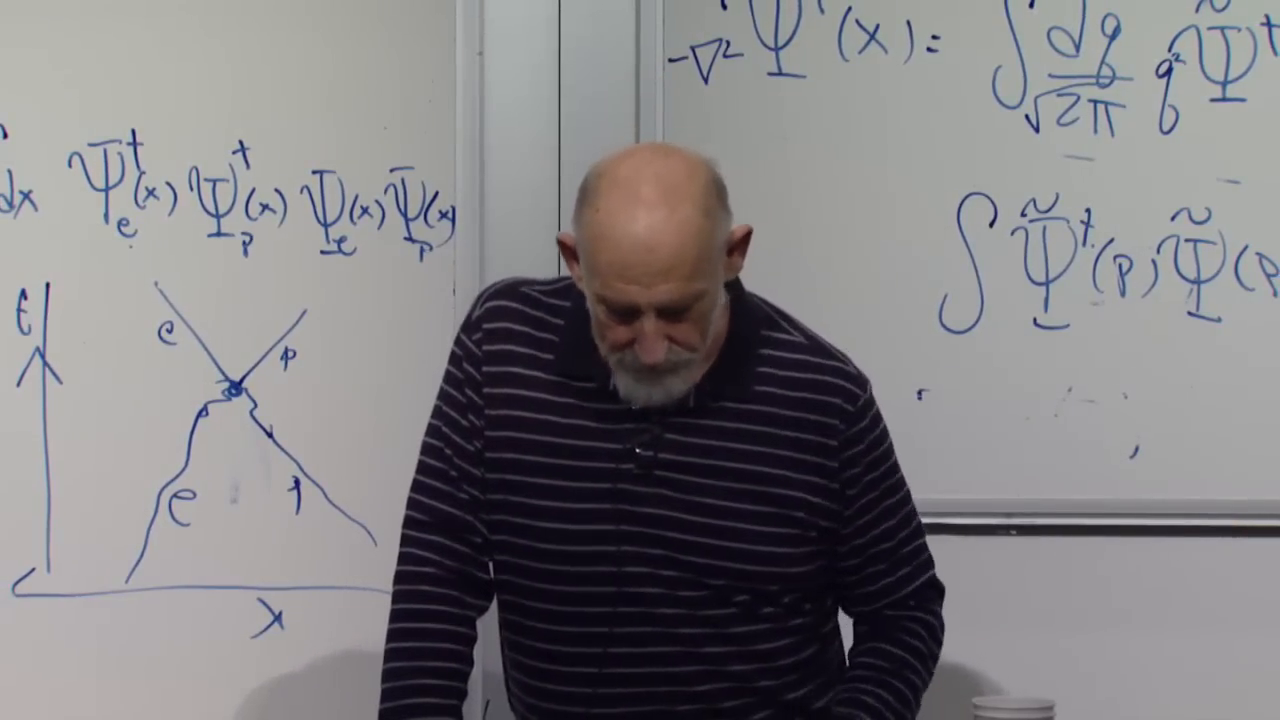
\includegraphics[width=0.94\linewidth]{lecture_09_frame_02.png}\caption{Die Kontaktwechselwirkung an der Tafel. Oberhalb der Raumzeit-Skizze stehen die vier lokalen Feldoperatoren; der Treffpunkt ist der einzige Ort, an dem die idealisierte Wechselwirkung wirkt.}\lectureframe{00:35:36}\end{figure}

\begin{figure}[htbp]\centering
\begin{tikzpicture}[x=1.2cm,y=1.0cm,>=Latex]
\draw[->] (-3.0,0) -- (3.0,0) node[right] {$x$};
\draw[->] (0,-0.2) -- (0,4.2) node[above] {$t$};
\coordinate (v) at (0,2.0);
\fill (v) circle (1.8pt);
\draw[thick,->] (-2.2,0.4) -- (v);
\draw[thick,->] (2.0,0.4) -- (v);
\draw[thick,->] (v) -- (-1.6,3.7);
\draw[thick,->] (v) -- (2.2,3.7);
\node[left] at (-1.65,0.7) {$e$};
\node[right] at (1.55,0.7) {$p$};
\node[left] at (-1.15,3.3) {$e$};
\node[right] at (1.65,3.3) {$p$};
\node[right] at (0.12,2.05) {$g$};
\end{tikzpicture}\caption{Eine klare Rekonstruktion des lokalen Streubildes. Der Vertex ist eine Kurzschreibweise für den Operator in Gl.~\eqref{eq:l9-contact}, kein klassisches Stoßgesetz.}\end{figure}

Reale Elektronen und Protonen wechselwirken über das Coulomb-Potential über eine gewisse Entfernung hinweg. Das Kontaktmodell ist lediglich ein erster, kleiner Schritt: Würde das Experiment zeigen, dass zwei Teilchensorten nur dann streuen, wenn sie sich überlappen, wäre Gl.~\eqref{eq:l9-contact} ein typischer Term, den wir in den Hamiltonoperator aufnehmen würden.

\begin{classroomqa}\lecturetimestamp{00:35:40}\audiencequestion{Warum gehört dieser Streuoperator zum Hamiltonoperator, wenn sich die Energie nicht ändert?}\lecturerresponse{Der Hamiltonoperator ist sowohl der Energieoperator als auch der Erzeuger der Zustandsänderung. Eine potentielle Energie zwischen den beiden Teilchen bewirkt Streuung während der zeitlichen Entwicklung. Die Erhaltung der Gesamtenergie bedeutet nicht, dass der Zustand oder die einzelnen Impulse der Teilchen unverändert bleiben.}\end{classroomqa}

Daraus ergibt sich eine praktische Regel. Zuerst ermitteln wir experimentell, welche lokalen Prozesse Teilchen durchlaufen können. Dann kodieren wir diese Prozesse in dem Operator, der den Zustand aktualisiert. Feldprodukte sind keine bloße algebraische Zierde: Ihre adjungierten und nicht adjungierten Faktoren legen fest, welche Teilchensorten auftreten und verschwinden.

\section{Zerfall, Umkehrprozess und Hermitizität}

Angenommen, in einer Blasenkammer endet die Spur einer Teilchensorte \(A\) an einem Punkt, von dem die Spuren \(B\) und \(C\) ausgehen. Der lokale Prozess lautet
\begin{equation}
A\longrightarrow B+C.
\end{equation}
Der Operator, der ihn bewirkt, ist
\begin{equation}
V=g\int dx\,
\psi_B^\dagger(x)\psi_C^\dagger(x)\psi_A(x).
\label{eq:l9-decay-half}
\end{equation}
Das Vernichtungsfeld entfernt \(A\); die beiden Erzeugungsfelder erzeugen \(B\) und \(C\) am selben Ort. Die Integration mit gleichem Gewicht über jedes \(x\) drückt räumliche Translationsinvarianz aus und liefert unmittelbar
\begin{equation}
p_A=p_B+p_C.
\end{equation}

Ein Hamiltonoperator muss hermitesch sein. Dadurch ist \(e^{-itH}\) unitär und die Gesamtwahrscheinlichkeit bleibt erhalten. Gleichung~\eqref{eq:l9-decay-half} ist für sich genommen nicht hermitesch, daher müssen wir ihren adjungierten Term hinzufügen:
\begin{equation}
H_{\mathrm{int}}
=\int dx\left[
g\,\psi_B^\dagger\psi_C^\dagger\psi_A
+g^*\,\psi_A^\dagger\psi_C\psi_B
\right](x).
\label{eq:l9-hermitian-vertex}
\end{equation}
Für eine reelle Kopplung \(g\) sind die beiden Koeffizienten gleich. Beim hermiteschen Konjugieren wird neben dem Austausch von adjungierten und nicht adjungierten Feldern auch die Operatorreihenfolge umgekehrt. In diesem bosonischen Spielzeugmodell kommutieren Felder verschiedener Teilchensorten, sodass diese Umordnung keine weitere Schwierigkeit mit sich bringt.

Der zweite Term beschreibt den umgekehrten Prozess,
\begin{equation}
B+C\longrightarrow A.
\end{equation}
Ein geschlossener, unitärer Hamiltonoperator, der den Zerfall zulässt, enthält also auch die Amplitude für die Rekombination. Das bedeutet nicht, dass beide Richtungen bei jeder Wahl der äußeren Impulse auftreten; Energieerhaltung und andere Erhaltungssätze können eine Richtung kinematisch unmöglich machen. Es bedeutet, dass sowohl der Operator als auch sein Adjungierter zur Dynamik gehören.

\begin{classroomqa}\lecturetimestamp{00:42:48}\audiencequestion{Kann es eine Ausnahme von der Regel geben, dass auch der umgekehrte Prozess möglich ist?}\lecturerresponse{Nicht bei einem hermiteschen Hamiltonoperator eines geschlossenen Systems: Die adjungierte Wechselwirkung ist erforderlich. Eine bestimmte Rückreaktion kann durch die Kinematik oder eine andere erhaltene Quantenzahl dennoch blockiert sein, aber das konjugierte Matrixelement ist vorhanden.}\end{classroomqa}

Die Zahl \(g\) ist die Kopplungskonstante. Ist \(g\) klein, wechselwirken Teilchen, die aufeinandertreffen, nur schwach; ist sie groß, ist die Übergangsamplitude größer. Kopplungskonstanten sind in der Regel experimentell bestimmte Parameter, obwohl Symmetrien mehrere scheinbar verschiedene Kopplungen miteinander verknüpfen können.

Dieselbe Grammatik lässt sich auf kompliziertere Reaktionen anwenden. Beim Betazerfall
\begin{equation}
n\longrightarrow p+e^-+\bar\nu_e,
\end{equation}
enthält ein schematischer lokaler Term vier Felder: Eines vernichtet das Neutron, drei erzeugen Proton, Elektron und Elektron-Antineutrino; hinzu kommt der hermitesch konjugierte Prozess. Schon daran ist zu erkennen, wie eine kleine Menge von Operator-Monomeren allmählich eine Quantenfeldtheorie definiert.

\section{Warum das Quadrat des Hamiltonoperators wichtig ist}

Die Kurzzeitformel \eqref{eq:l9-short-update} berücksichtigte nur die erste Ordnung in \(\epsilon\). Die vollständige Entwicklung lautet
\begin{equation}
e^{-i\epsilon H}
=1-i\epsilon H-\frac{\epsilon^2}{2}H^2
+\frac{i\epsilon^3}{3!}H^3+\cdots.
\label{eq:l9-exponential}
\end{equation}
In zweiter Ordnung wirkt der Hamiltonoperator zweimal. Das ist der algebraische Ursprung der ersten zusammengesetzten Prozessbilder.

Beim Vertex \(A\leftrightarrow B+C\) kann eine Wirkung \(B+C\) zu \(A\) verbinden und eine zweite dieses \(A\) wieder in \(B+C\) zerlegen:
\begin{equation}
B+C\longrightarrow A\longrightarrow B+C.
\label{eq:l9-bc-scattering}
\end{equation}
Der Gesamtbeitrag ist eine Streuamplitude \(B+C\to B+C\). Das Zwischenzustands-\(A\) ist kein zusätzliches beobachtetes Ereignis; es bezeichnet den Zustand, über den zwischen den beiden Wirkungen der Wechselwirkung summiert wird.

\begin{classroomqa}\lecturetimestamp{00:49:54}\audiencequestion{Muss das \(C\)-Feld im hingeschriebenen Produkt zweiter Ordnung adjungiert sein?}\lecturerresponse{Ja, die Operatorreihenfolge muss der angegebenen Abfolge entsprechen. Der erste Vertex vernichtet \(B\) und \(C\) und erzeugt \(A\); der zweite vernichtet \(A\) und erzeugt erneut \(B\) und \(C\). Mit den entsprechenden Adjungierten ist diese Deutung wiederhergestellt.}\end{classroomqa}

\begin{figure}[htbp]\centering
\includegraphics[width=0.94\linewidth]{lecture_09_frame_05.png}\caption{Die beiden Orientierungen des elementaren \(A\leftrightarrow B+C\)-Vertex an der Tafel. Ihre Kombination ist die bildliche Kurzschreibweise für den Prozess zweiter Ordnung in Gl.~\eqref{eq:l9-bc-scattering}.}\lectureframe{00:48:56}\end{figure}

Nun kommt ein Zuschauer-\(B\) hinzu. Eine Wirkung lässt \(A\) \(C\) emittieren und zu \(B\) werden; eine spätere Wirkung lässt dieses \(C\) sich mit dem ursprünglichen \(B\) verbinden, sodass \(A\) entsteht. Die äußeren Teilchen sind wieder \(A+B\), doch ihre Impulse können sich ändern. Wir beschreiben dies als Streuung von \(A\) und \(B\) durch den Austausch von \(C\).

\begin{figure}[htbp]\centering
\includegraphics[width=0.94\linewidth]{lecture_09_frame_06.png}\caption{Die Austausch-Konstruktion an der Tafel. Im Diagramm rechts verbinden eine interne \(C\)-Linie und zwei elementare Vertices die Streuung der äußeren \(A\)- und \(B\)-Teilchen.}\lectureframe{00:51:22}\end{figure}

\begin{figure}[htbp]\centering
\begin{tikzpicture}[x=1.1cm,y=1cm,>=Latex]
\draw[->] (-3.7,-0.2) -- (-3.7,4.2) node[above] {$t$};
\coordinate (v1) at (-0.9,1.25);
\coordinate (v2) at (0.9,2.95);
\fill (v1) circle (1.7pt);
\fill (v2) circle (1.7pt);
\draw[thick,->] (-2.6,0.2) -- (v1) node[midway,below left] {$A$};
\draw[thick,->] (2.6,0.2) -- (v2) node[midway,below right] {$B$};
\draw[thick,->] (v1) -- (-2.4,4.0) node[midway,left] {$B$};
\draw[thick,->] (v2) -- (2.5,4.0) node[midway,right] {$A$};
\draw[thick,->,dashed] (v1) -- (v2) node[midway,above left] {$C$};
\node[below] at (0,-0.05) {$A+B\rightarrow A+B$};
\end{tikzpicture}\caption{Eine klare Rekonstruktion des \(C\)-Austauschs. Jeder Punkt liefert einen Faktor \(g\), daher ist dieser Beitrag zweiter Ordnung proportional zu \(g^2\).}\end{figure}

Jeder lokale Wechselwirkungspunkt heißt Vertex. Jeder Vertex trägt einen Faktor seiner Kopplung bei. Ein Beitrag mit zwei Vertices enthält also \(g^2\), einer mit drei Vertices \(g^3\) und so weiter. Ein einziger Term im Hamiltonoperator korreliert somit eine große Familie von Reaktionen. Diese Ökonomie ist ein Grund für die große Leistungsfähigkeit der Quantenfeldtheorie: Eine kleine Zahl lokaler Wechselwirkungen ordnet eine enorme Menge von Streudaten.

\begin{classroomqa}\lecturetimestamp{00:53:14}\audiencequestion{Wie nennt man den Prozess \(A\to B+C\to A\)?}\lecturerresponse{Es handelt sich um einen Selbstenergiebeitrag. Ein beobachtetes \(A\) ist nicht einfach der ungestörte Einteilchen-Basiszustand; der Wechselwirkungszustand enthält auch Amplituden für nahegelegene \(B+C\)-Komponenten. Streuung daran kann diese bekleidete Struktur sichtbar machen.}\end{classroomqa}

Die Quantenelektrodynamik liefert das vertraute Beispiel. Ein lokaler Elektron--Photon-Vertex kann ein Elektron vernichten, ein Elektron neu erzeugen und ein Photon erzeugen. In zweiter Ordnung kann das Elektron ein Photon emittieren und wieder absorbieren. Es liegt nahe, dies als winzigen Film zu erzählen, doch seine präzise Bedeutung ist ein Term in der Störungsentwicklung. Das physikalische Elektron ist ein bekleideter Zustand mit Komponenten, die Photonen enthalten.

Die Abschätzung aus der Vorlesung, diese Komponente betrage ``etwa ein Prozent'', vermittelt die Größenordnung, die durch die Feinstrukturkonstante \(\alpha_{\mathrm{em}}\simeq 1/137\) festgelegt wird. Eine präzise Wahrscheinlichkeit für eine Photon-Fock-Komponente hängt von der Energieauflösung und davon ab, wie der Wechselwirkungszustand definiert wird; sie ist keine universelle Ein-Prozent-Eigenschaft eines isolierten Elektrons. Die belastbare Aussage ist, dass die Wechselwirkung die messbare Struktur des Elektrons verändert.

\section{Was ein Diagramm aussagt und was nicht}

Die Diagramme sind eine rechnerische Kurzschreibweise für Potenzen des Wechselwirkungs-Hamiltonoperators. Sie sind keine verlässlichen klassischen Abläufe, in denen ein Teilchen eindeutig erst ein Ereignis und dann ein anderes durchläuft. Wenn man hineinschaut, um zu entscheiden, was ``wirklich geschehen'' ist, verändert man das Experiment und zerstört die kohärente Summe, wie bei gewöhnlicher Quanteninterferenz.

\begin{classroomqa}\lecturetimestamp{00:56:52}\audiencequestion{Sind an jedem Vertex sowohl Energie als auch Impuls erhalten?}\lecturerresponse{Bei der hier durchgeführten Hamilton-Konstruktion zu gleichen Zeiten ergibt das räumliche Integral unmittelbar eine Impuls-Deltafunktion. Für diese einzelne Einfügung hat noch kein Zeitintegral eine Energie-Deltafunktion geliefert. Die vollständige, translationsinvariante Streuamplitude erhält die Gesamtenergie, während interne Linien nicht der On-Shell-Beziehung beobachteter Teilchen entsprechen müssen. In der kovarianten Diagrammsprache ist der Viererimpuls an jedem Vertex erhalten, interne Teilchen können jedoch off shell sein.}\end{classroomqa}

Die scheinbar fehlende Energie in einem naiven Vertexbild ist ein weiterer Grund, die Wechselwirkungsenergie nicht zu vernachlässigen. Der gesamte Hamiltonoperator ist mehr als die Summe der Energien freier Teilchen. Falls Verwirrung entsteht, kehren wir zu Gl.~\eqref{eq:l9-exponential} zurück: Das Bild steht für einen Term in der Entwicklung der unitären zeitlichen Entwicklung. Die vollständige Feynman-Diagrammtechnik liefert systematische Zeitordnung, Propagatoren, Integrationen und Symmetriefaktoren, doch die grundlegende Physik beginnt bereits hier.

Eine weiterführende Frage nimmt das Diagramm zu wörtlich und vergleicht das emittierte Photon mit dem elektrischen Feld, das ein langsam bewegtes Elektron umgibt.

\begin{classroomqa}\lecturetimestamp{00:58:26}\audiencequestion{Wird das elektrische Feld des Elektrons in einiger Entfernung tatsächlich von ausgestrahlten Photonen erzeugt? Wie passt das zu Interferenz und zum Aharon---Bohm-Effekt?}\lecturerresponse{Ein statisches Feld oder ein Induktionsfeld ist kein Strom realer ausgestrahlter Photonen. Die Quantenelektrodynamik beschreibt sowohl Strahlung als auch die elektromagnetische Bekleidung des Elektrons mit demselben Feld, doch die zugehörigen Quantenzustände und die Kinematik unterscheiden sich. Bei einem ultrarelativistischen Elektron lassen sich manche Feldkomponenten sinnvoll als Strom nahezu reeller Photonen auffassen; bei einem langsamen Elektron ist eine wörtliche Photonentrajektorie das falsche Modell. Der Doppelspaltversuch und der Aharon---Bohm-Effekt sind ebenfalls nichtklassische Feldphänomene, machen dieses Selbstenergie-Diagramm aber nicht zu einem mechanischen Film.}\end{classroomqa}

\begin{classroomqa}\lecturetimestamp{01:01:28}\audiencequestion{Warum scheitert ein klassisches Modell des Diagramms genau?}\lecturerresponse{Weil die Rechnung die Amplituden aller zulässigen Zwischenalternativen kohärent addiert. Die Erfahrung macht die Bilder anschaulich, doch ihr wörtlicher Gehalt geht nie über die Operatorentwicklung hinaus, durch die sie definiert sind. Sie sind eine kompakte Methode, \(H^2,H^3,\ldots\) zu berechnen, keine Aufzeichnung beobachteter Zwischenereignisse.}\end{classroomqa}

\begin{classroomqa}\lecturetimestamp{01:03:04}\audiencequestion{Kann die gewöhnliche Coulomb-Wechselwirkung als klassischer Grenzfall des Photonenaustauschs entstehen?}\lecturerresponse{Ja. Wertet man die entsprechende photonvermittelte Amplitude aus und nimmt den nichtrelativistischen statischen Grenzfall, erhält man das Coulomb-Potential. Die Herleitung ist technischer als die vorliegende Operator-Skizze und sollte dennoch nicht so verstanden werden, als spränge ein Photon buchstäblich zwischen zwei klassischen Teilchen hin und her.}\end{classroomqa}

\begin{classroomqa}\lecturetimestamp{01:03:44}\audiencequestion{Werden Kopplungskonstanten aus den Feldprodukten berechnet?}\lecturerresponse{Ihre Zahlenwerte sind gewöhnlich experimentelle Eingangsgrößen. Symmetrien können sie einschränken oder Kopplungen miteinander verknüpfen, die andernfalls unabhängig wären. Wenn eine solche Beziehung die relativen Stärken verschiedener Reaktionen vorhersagt und das Experiment sie bestätigt, ist diese Übereinstimmung besonders aufschlussreich.}\end{classroomqa}

\begin{classroomqa}\lecturetimestamp{01:04:48}\audiencequestion{Welche Rolle spielt eine zufällige Symmetrie im Vergleich zu einer Eichsymmetrie?}\lecturerresponse{Eine Eichsymmetrie schränkt unmittelbar die zulässige Struktur und die Beziehungen zwischen Kopplungen ein. Eine zufällige Symmetrie wird nicht auf fundamentaler Ebene auferlegt, sondern entsteht, weil zufällig alle zulässigen Wechselwirkungen niedriger Ordnung sie respektieren. Sie kann dennoch wichtige Folgen haben, auch wenn ihr Ursprung und ihre Robustheit sich von denen einer Eichsymmetrie unterscheiden.}\end{classroomqa}

Damit lassen wir die nichtrelativistische Feldtheorie vorerst hinter uns. Wir haben Fermionen angekündigt. Statt sie sofort zweitzuquantisieren, wollen wir zunächst die relativistische Einteilchengleichung verstehen, der ihre Feldoperatoren genügen müssen.

\section{Warum das Elektron eine relativistische Beschreibung erfordert}

Wir beginnen mit einer räumlichen Dimension. Das ist keine realistische Einschränkung, beseitigt aber die geometrische Komplexität des dreidimensionalen Spins, während die wesentliche Algebra erhalten bleibt. Das Elektron ist leicht genug, dass relativistische Effekte bereits in Atomen eine Rolle spielen. In Wasserstoff beträgt seine charakteristische Geschwindigkeit etwa
\begin{equation}
v\sim\alpha_{\mathrm{em}}c\approx 0.007c,
\end{equation}
also ungefähr ein Prozent der Lichtgeschwindigkeit. Bei inneren Elektronen eines schweren Atoms liegt die grobe Größenordnung bei \(v\sim Z\alpha_{\mathrm{em}}c\), sodass relativistische Korrekturen erheblich sein können. Ob historische Neugier oder die für die Atomphysik erforderliche Genauigkeit den entscheidenden Anstoß gab: Eine relativistische Gleichung vom Schr\"odinger-Typ ist physikalisch notwendig.

Das übliche Quantisierungsrezept geht von der klassischen Beziehung zwischen Energie und Impuls aus. Nichtrelativistisch gilt
\begin{equation}
E=\frac{p^2}{2m},
\end{equation}
und die Ersetzungen
\begin{equation}
E\mapsto i\partial_t,
\qquad
p\mapsto-i\partial_x
\end{equation}
ergeben
\begin{equation}
i\partial_t\varphi(x,t)
=-\frac{1}{2m}\partial_x^2\varphi(x,t).
\end{equation}

Die Relativitätstheorie liefert dagegen mit \(c=1\)
\begin{equation}
E^2=p^2+m^2.
\label{eq:l9-rel-dispersion}
\end{equation}

\begin{figure}[htbp]\centering
\includegraphics[width=0.94\linewidth]{lecture_09_frame_07.png}\caption{Der Übergang an der Tafel von \(E=p^2/2m\) zur relativistischen Beziehung \(E^2=p^2+m^2\), mit \(c=1\).}\lectureframe{01:10:30}\end{figure}

Wenden wir die Ersetzungen auf die quadrierte Beziehung an, erhalten wir
\begin{equation}
-\partial_t^2\varphi
=\left(-\partial_x^2+m^2\right)\varphi,
\label{eq:l9-klein-gordon}
\end{equation}
oder äquivalent
\begin{equation}
\left(\partial_t^2-\partial_x^2+m^2\right)\varphi=0.
\end{equation}
Dies ist die Klein---Gordon-Gleichung. Sie ist eine durchaus sinnvolle relativistische Feldgleichung, insbesondere für Felder mit Spin null. Die gesuchte Elektronengleichung soll jedoch erster Ordnung in der Zeit sein,
\begin{equation}
i\partial_t\Psi=H\Psi,
\end{equation}
sodass \(H\) selbst die zeitliche Entwicklung erzeugt und nicht nur \(H^2\).

Formal könnte man
\begin{equation}
H=\sqrt{-\partial_x^2+m^2}.
\end{equation}
wählen. Die Wurzel lässt sich im Impulsraum eindeutig definieren, wo sie mit \(\sqrt{p^2+m^2}\) multipliziert, doch im Ortsraum ist sie ein nichtlokaler pseudodifferentieller Operator. Mathematisch ist das sinnvoll, für die lokale Gleichung, die wir suchen, aber ästhetisch unbefriedigend. Deshalb beginnen wir noch einmal von vorn.

\section{Eine masselose Welle, die sich nach rechts bewegt}

Betrachten wir zunächst ein masseloses Teilchen, das sich nach rechts bewegt. Für seine positive Energie und seinen Impuls gilt
\begin{equation}
E=p
\qquad (c=1).
\end{equation}
Die Quantisierung ergibt
\begin{equation}
i\partial_t\psi=-i\partial_x\psi,
\end{equation}
oder
\begin{equation}
(\partial_t+\partial_x)\psi=0.
\label{eq:l9-right-mover}
\end{equation}
Jede Lösung hat die Form
\begin{equation}
\psi(x,t)=f(x-t).
\end{equation}
Das Profil bleibt unverändert und bewegt sich mit Lichtgeschwindigkeit nach rechts.

Dabei treten sofort zwei Schwierigkeiten auf. Erstens hat ein negativer Impuls, wenn Gl.~\eqref{eq:l9-right-mover} auf beliebige Fourier-Moden wirken darf, die Energie \(E=p<0\); der Hamiltonoperator ist dann nach unten nicht beschränkt. Eine willkürliche Beschränkung auf \(p>0\) würde nur rechtslaufende Moden beibehalten und ergäbe noch nicht die gesuchte Elektronentheorie. Zweitens ist die Gleichung eine Einbahnstraße: Sie enthält kein gewöhnliches linkslaufendes Elektron. Zunächst lösen wir das Links-rechts-Problem und lassen die negativen Energien außer Betracht.

\section{Zwei Komponenten und die Alpha-Matrix}

Wir führen zwei Amplituden ein,
\begin{equation}
\Psi(x,t)=
\begin{pmatrix}
\psi_1(x,t)\\[3pt]
\psi_2(x,t)
\end{pmatrix},
\end{equation}
wobei \(\psi_1\) im masselosen Grenzfall nach rechts und \(\psi_2\) nach links läuft:
\begin{align}
(\partial_t+\partial_x)\psi_1&=0,
&
(\partial_t-\partial_x)\psi_2&=0.
\end{align}
Die Quantenmechanik erlaubt zudem beliebige Überlagerungen der beiden. Ein Teilchen kann daher Amplituden für beide Richtungen haben, statt ein für alle Mal ein klassisches Etikett zu tragen.

Dieser zusätzliche zweifachwertige Freiheitsgrad ähnelt algebraisch dem Spin, ist aber in einer Dimension kein gewöhnlicher Drehimpuls. Definieren wir
\begin{equation}
\alpha=
\begin{pmatrix}
1&0\\
0&-1
\end{pmatrix}
=\sigma_3.
\label{eq:l9-alpha}
\end{equation}
Der Eigenvektor zum Eigenwert \(+1\) wählt die rechts laufende Komponente aus, der zum Eigenwert \(-1\) die links laufende. In der masselosen Theorie lautet der Hamiltonoperator einfach
\begin{equation}
H=\alpha p,
\end{equation}
und die beiden Gleichungen lassen sich zu einer einzigen zusammenfassen:
\begin{equation}
i\partial_t\Psi=-i\alpha\partial_x\Psi.
\label{eq:l9-massless-dirac}
\end{equation}

\begin{classroomqa}
\lecturetimestamp{01:22:44}
\audiencequestion{Wie heißt die Diagonalmatrix, die die beiden Komponenten unterscheidet?}
\lecturerresponse{Als Pauli-Matrix ist sie \(\sigma_3\), nicht \(\sigma_1\). In der Dirac-Notation für die vorliegende Konstruktion nennen wir sie \(\alpha\). Ihre Algebra ist die bekannte Pauli-Algebra, obwohl sie hier die Richtung und nicht den Drehimpuls bezeichnet.}
\end{classroomqa}

\begin{classroomqa}
\lecturetimestamp{01:23:32}
\audiencequestion{Erhält die Konstruktion in drei Dimensionen, wo die Richtung ein Vektor ist, eine stärker geometrische Bedeutung?}
\lecturerresponse{Ja. Das dreidimensionale Problem erfordert eine Matrix für jede Raumrichtung und führt zu einer reichhaltigeren Spinorstruktur. Das eindimensionale Modell ist in seinem eigenen Rahmen dennoch exakt und isoliert die wesentliche Links-rechts-Algebra, ohne diese zusätzliche Komplexität.}
\end{classroomqa}

\begin{figure}[htbp]
\centering
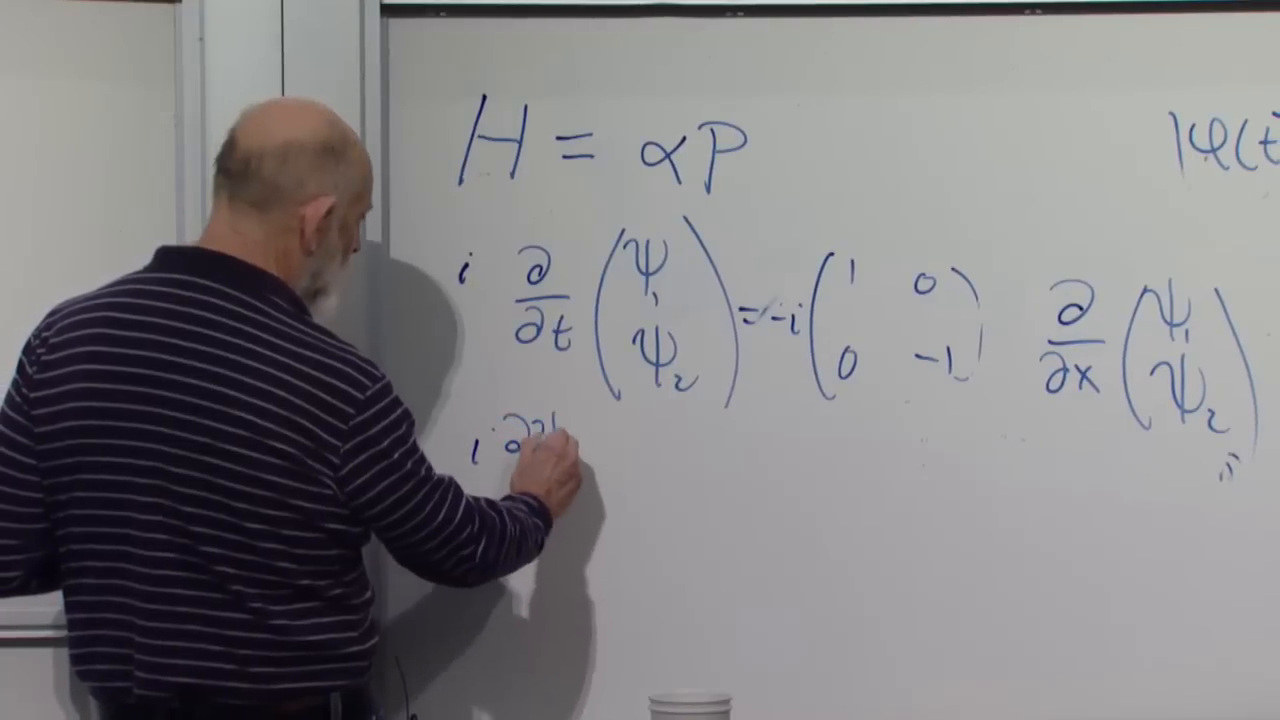
\includegraphics[width=0.94\linewidth]{lecture_09_frame_03.png}
\caption{Die masselose Zweikomponentengleichung an der Tafel: \(H=\alpha P\); die Diagonalmatrix ordnet \(\psi_1\) und \(\psi_2\) entgegengesetzte Ausbreitungsrichtungen zu.}
\lectureframe{01:26:00}
\end{figure}

Das Problem der Bewegung nur in eine Richtung ist behoben. Das Spektrum negativer Energien bleibt bestehen, und wir haben einen dritten Mangel entdeckt: Die beiden Komponenten sind weiterhin masselos und breiten sich mit Lichtgeschwindigkeit aus. Im nächsten Schritt müssen eine Ruheenergie eingeführt und die Richtungen gekoppelt werden.

\section{Masse hinzufügen und die Dirac-Algebra entdecken}

Fügen wir den allgemeinsten einfachen, zur Masse proportionalen Term hinzu:
\begin{equation}
H=\alpha p+\beta m,
\label{eq:l9-dirac-hamiltonian}
\end{equation}
wobei \(\beta\) nur auf den zweikomponentigen Index wirkt. Es hätte die Einheitsmatrix oder eine andere Matrix sein können; wir lassen die relativistische Dispersionsrelation entscheiden.

Da \(H^2\) gleich \(p^2+m^2\) sein muss, quadrieren wir Gl.~\eqref{eq:l9-dirac-hamiltonian}:
\begin{align}
H^2
&=(\alpha p+\beta m)^2\\
&=\alpha^2p^2+\beta^2m^2
+(\alpha\beta+\beta\alpha)pm.
\label{eq:l9-square-dirac}
\end{align}
Die Matrizen kommutieren mit \(p\), weil sie auf den internen zweikomponentigen Raum wirken, während \(p\) auf die räumliche Wellenfunktion wirkt. Damit Gl.~\eqref{eq:l9-rel-dispersion} erfüllt ist, muss gelten:
\begin{equation}
\alpha^2=\mathbb{1},
\qquad
\beta^2=\mathbb{1},
\qquad
\{\alpha,\beta\}
=\alpha\beta+\beta\alpha=0.
\label{eq:l9-dirac-algebra}
\end{equation}
Die erste Bedingung ist für \(\alpha=\sigma_3\) bereits erfüllt. Jede andere Pauli-Matrix antikommutiert mit ihr und hat das Quadrat der Einheitsmatrix. Wir wählen
\begin{equation}
\beta=
\begin{pmatrix}
0&1\\
1&0
\end{pmatrix}
=\sigma_1.
\label{eq:l9-beta}
\end{equation}
Die Wahl von \(\sigma_1\) statt \(\sigma_2\) ist eine Konvention für die Basis; nach einer unitären Basisänderung realisieren beide dieselbe Algebra.

\begin{classroomqa}
\lecturetimestamp{01:33:00}
\audiencequestion{Hat Dirac einfach erkannt, dass Pauli-Matrizen diese algebraischen Bedingungen erfüllen?}
\lecturerresponse{Die historische Herleitung wurde direkt in drei Dimensionen durchgeführt und führte Matrizen ein, die die erforderlichen Relationen erfüllen. Sobald die Bedingungen formuliert sind, ergibt sich die eindimensionale Lösung unmittelbar aus der Pauli-Algebra: Man wählt zwei verschiedene Pauli-Matrizen.}
\end{classroomqa}

\begin{classroomqa}
\lecturetimestamp{01:34:24}
\audiencequestion{Ist dieses \(\beta\) der relativistische Geschwindigkeitsparameter \(v/c\)?}
\lecturerresponse{Nein. Es ist eine Matrix, die auf die Spinorkomponenten wirkt. Der wiederverwendete Buchstabe ist lediglich Diracs Notation; mit der kinematischen Größe \(v/c\) hat er nichts zu tun.}
\end{classroomqa}

In drei Raumdimensionen reichen \(2\times2\)-Matrizen für den vollständigen Satz der erforderlichen antikommutierenden Matrizen nicht aus. Diese Erweiterung wird auf später verschoben. In einer Dimension genügen die Gleichungen ~\eqref{eq:l9-alpha} und \eqref{eq:l9-beta}.

\section{Die gekoppelte eindimensionale Dirac-Gleichung}

Setzen wir \(p=-i\partial_x\) ein, erhalten wir die eindimensionale Dirac-Gleichung in Hamilton-Form:
\begin{equation}
i\partial_t\Psi
=\left(-i\alpha\partial_x+\beta m\right)\Psi.
\label{eq:l9-one-dimensional-dirac}
\end{equation}
Da \(\alpha\) diagonal ist, lässt ihr Ableitungsterm die beiden Komponenten getrennt. Da \(\beta\) nicht diagonal ist, vertauscht der Massenterm sie. In Komponenten geschrieben:
\begin{align}
i\partial_t\psi_1
&=-i\partial_x\psi_1+m\psi_2,
\label{eq:l9-dirac-component-one}\\
i\partial_t\psi_2
&=+i\partial_x\psi_2+m\psi_1.
\label{eq:l9-dirac-component-two}
\end{align}

\begin{figure}[htbp]
\centering
\includegraphics[width=0.94\linewidth]{lecture_09_frame_08.png}
\caption{Die gekoppelten Komponentengleichungen an der Tafel. Die entgegengesetzten Vorzeichen der Ableitungen kodieren die Rechts- und Linksbewegung; der nichtdiagonale Massenterm vertauscht \(\psi_1\) und \(\psi_2\).}
\lectureframe{01:37:44}
\end{figure}

Sobald \(m\ne0\), entwickeln sich die Komponenten nicht mehr unabhängig voneinander. Durch Quadrieren der Gleichung erster Ordnung erhält man für jede Komponente den Klein--Gordon-Operator:
\begin{equation}
\left(\partial_t^2-\partial_x^2+m^2\right)\psi_a=0,
\qquad a=1,2,
\end{equation}
Für ebene Wellen gilt \(E^2=p^2+m^2\). Ihre Gruppengeschwindigkeit ist
\begin{equation}
v_g=\frac{dE}{dp}=\frac{p}{E},
\end{equation}
und ihr Betrag ist bei von null verschiedener Masse kleiner als eins.

Der Zusammenhang zwischen Masse und Mischung der Links- und Rechtskomponenten ist kein Zufall. Ein masseloser Rechtshänder bleibt unter jeder eigentlichen Lorentz-Boost-Transformation ein Rechtshänder; kein Beobachter mit unterlichtschneller Geschwindigkeit kann das Licht überholen und seine Richtung umkehren. Ein massives Teilchen lässt sich in sein Ruhesystem überführen. Betrachtet man es dann aus einem schnelleren Bezugssystem, das sich in derselben Richtung bewegt, erscheint seine Geschwindigkeit umgekehrt. Eine relativistische Theorie mit Masse kann die rechts und links laufenden Sektoren daher nicht dauerhaft getrennt halten. Der nichtdiagonale Massenterm liefert genau die erforderliche Kopplung.

\begin{classroomqa}
\lecturetimestamp{01:40:01}
\audiencequestion{Ist der Austausch der beiden Komponenten eine chirale Oszillation?}
\lecturerresponse{In dieser eindimensionalen Basis unterscheidet \(\alpha\) die beiden masselosen chiralen Richtungen. Der Massenterm ist nichtdiagonal und mischt sie, sodass die Chiralität nicht mehr erhalten ist. In diesem Sinne ist der Massenterm die Ursache der chiralen Oszillation.}
\end{classroomqa}

\begin{classroomqa}
\lecturetimestamp{01:40:46}
\audiencequestion{Warum sollte eine Fermionengleichung die Quadratwurzel einer Bosonengleichung sein?}
\lecturerresponse{Das sollte man nicht so verstehen. Die Dispersionsrelation \(E^2=p^2+m^2\) gilt für jedes freie relativistische Teilchen, unabhängig von seiner Statistik. Der Dirac-Operator liefert zufällig eine Matrixfaktorisierung des Klein--Gordon-Operators, aber aus dieser algebraischen Beziehung werden keine Fermionen aus Bosonen hergeleitet.}
\end{classroomqa}

\begin{classroomqa}
\lecturetimestamp{01:41:31}
\audiencequestion{Lässt sich die Gleichung in eine einfache skalare Faktorisierung in getrennte links und rechts laufende Faktoren zerlegen?}
\lecturerresponse{Nur im masselosen Grenzfall entkoppeln sich die beiden chiralen Gleichungen zu unabhängigen skalaren Faktoren. Für \(m\ne0\) ist die nützliche Faktorisierung matrixwertig: Die antikommutierenden Matrizen \(\alpha\) und \(\beta\) beseitigen den unerwünschten Mischterm.}
\end{classroomqa}

\begin{classroomqa}
\lecturetimestamp{01:42:04}
\audiencequestion{Bilden diese beiden gekoppelten Gleichungen bereits die Dirac-Gleichung?}
\lecturerresponse{Ja. Zusammen bilden sie die Dirac-Gleichung in einer Raumdimension, äquivalent zur kompakten Form in Gl.~\eqref{eq:l9-one-dimensional-dirac}. Eine symmetrischere kovariante Notation erhält man durch Multiplikation mit \(\beta\); diese Form behandeln wir jedoch später.}
\end{classroomqa}

Zwei Aufgaben bleiben bewusst ungelöst. Die Konstruktion hat die negativen Energien nicht beseitigt; sie hat negative Energielösungen in beiden Richtungssektoren geliefert, sodass dieses Problem nun deutlicher hervortritt. Außerdem lebt die Theorie weiterhin in einer Raumdimension. Die Interpretation der negativen Energielösungen und die Erweiterung der Matrixalgebra auf \(3+1\) Dimensionen sind die nächsten Schritte.

\chapter{Fermionen, Dirac-Matrizen und das Dirac-Meer}

Das Dirac-Meer ist unser Ziel, doch auch der Weg dorthin ist wichtig. Bevor wir uns der negativen Energie in der relativistischen Elektronentheorie zuwenden, benötigen wir zwei mathematische Werkzeuge. Zunächst betrachten wir die Operatoralgebra, die Fermionen von Bosonen unterscheidet. Danach wiederholen wir die eindimensionale Dirac-Gleichung, in der sich jede Erweiterung der Wellenfunktion erkennen lässt, ohne dass die Geometrie dreier Raumdimensionen hinzukommt. Sind diese Grundlagen geschaffen, erzwingt die dreidimensionale Gleichung ihre eigene Matrixstruktur. Die einleitende Betrachtung besetzter und leerer Fermionenzustände wird dann als Schlüssel zum Verständnis der Positronen wieder aufgegriffen.

Wir verwenden \(c=\hbar=1\). Das große \(P\) bezeichnet einen Impulsoperator, das kleine \(p\) einen Impulseigenwert und die fettgedruckten Symbole deren dreidimensionale Versionen.

\section{Austausch wird zur Operatoralgebra}

Betrachten wir zwei identische Teilchen, eines bei \(x\) und eines bei \(y\). Die Bezeichnungen \(x\) und \(y\) stehen für vollständige Ortsangaben; sie sind nicht zwei kartesische Koordinaten eines einzelnen Teilchens. Die Wirkung zweier Erzeugungsoperatoren auf das Vakuum ergibt
\begin{equation}
\lvert x,y\rangle
=
\psi^\dagger(x)\psi^\dagger(y)\lvert0\rangle.
\label{eq:l10-two-particle-state}
\end{equation}

Bei Bosonen bleibt der Zustand beim Vertauschen der beiden Plätze unverändert:
\begin{equation}
\lvert x,y\rangle=\lvert y,x\rangle.
\end{equation}
Die Operatorgleichung, die diese Symmetrie sicherstellt, lautet
\begin{equation}
\psi^\dagger(x)\psi^\dagger(y)
=
\psi^\dagger(y)\psi^\dagger(x).
\label{eq:l10-boson-exchange}
\end{equation}
Zwei bosonische Erzeugungsoperatoren kommutieren. Daher können wir ihre Reihenfolge umkehren, ohne den von ihnen erzeugten Zustand zu ändern.

Bei Fermionen ändert der Austausch das Vorzeichen:
\begin{equation}
\lvert x,y\rangle=-\lvert y,x\rangle.
\label{eq:l10-fermion-state-exchange}
\end{equation}
Das Gesamtvorzeichen eines einzelnen Zustandsvektors ist nicht beobachtbar, relative Vorzeichen zwischen Alternativen hingegen schon. Deshalb muss dieses Minuszeichen durchgehend beibehalten werden. Gleichung~\eqref{eq:l10-fermion-state-exchange} verlangt
\begin{equation}
\psi^\dagger(x)\psi^\dagger(y)
=
-\,\psi^\dagger(y)\psi^\dagger(x).
\label{eq:l10-fermion-operator-exchange}
\end{equation}

\begin{figure}[htbp]
\centering
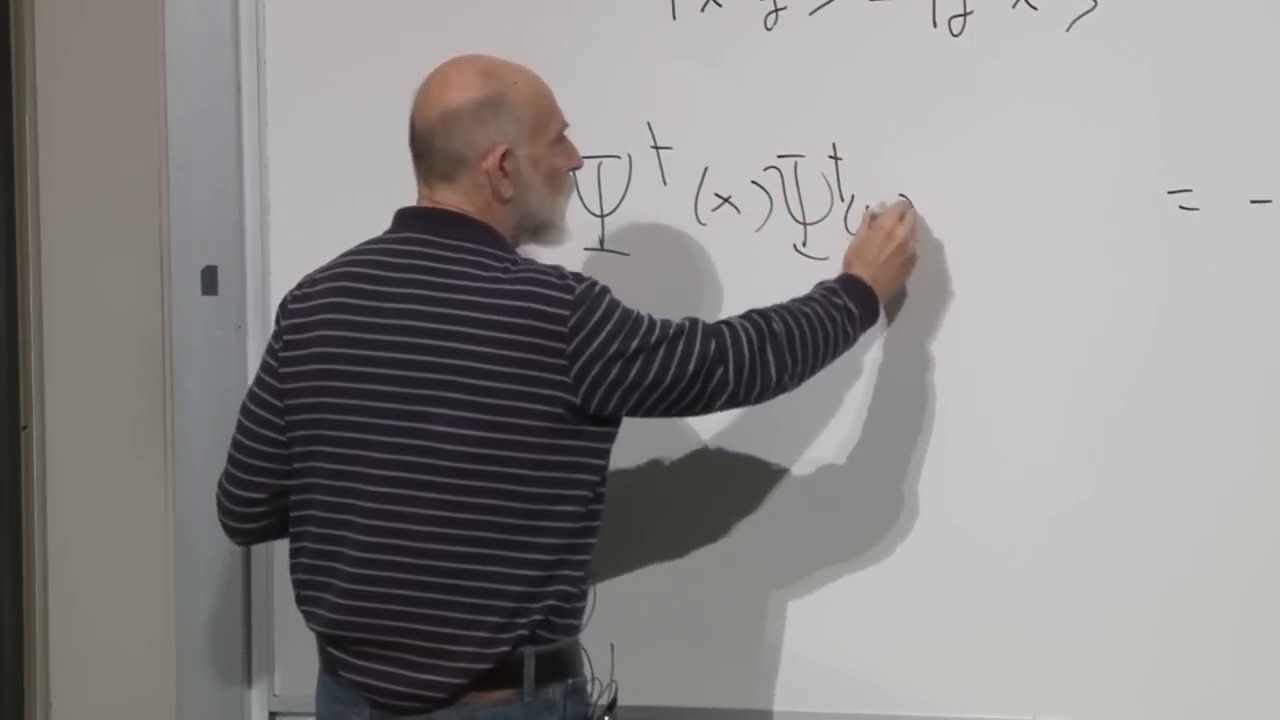
\includegraphics[width=0.94\linewidth]{lecture_10_figure_02.png}
\caption{Die Tafelgleichung, die den Austausch von Fermionen beschreibt. Beim Vertauschen der Erzeugungsoperatoren ändert der Zweiteilchenzustand sein Vorzeichen.}
\lectureframe{00:05:50}
\end{figure}

Für zwei beliebige Operatoren \(A\) und \(B\) definieren wir den Antikommutator durch
\begin{equation}
\{A,B\}:=AB+BA.
\end{equation}
Die Austauscherelation lautet folglich
\begin{equation}
\{\psi^\dagger(x),\psi^\dagger(y)\}=0.
\label{eq:l10-creation-anticommutator}
\end{equation}
In der entsprechenden Fermionenfeldalgebra treten an die Stelle der bosonischen Kommutatoren Antikommutatoren. Die beiden Verwendungen des Wortes „antikommutieren“ müssen auseinandergehalten werden: Feldoperatoren antikommutieren aufgrund der Fermi-Statistik, während Matrizen später antikommutieren, damit sich die Kreuzterme in einer relativistischen Dispersionsrelation aufheben.

Setzen wir nun \(y=x\) in Gleichung~\eqref{eq:l10-creation-anticommutator} ein. Beide Produkte sind dann gleich:
\begin{align}
0
&=\{\psi^\dagger(x),\psi^\dagger(x)\}\\
&=2\,\psi^\dagger(x)\psi^\dagger(x).
\end{align}
Also gilt
\begin{equation}
\bigl(\psi^\dagger(x)\bigr)^2=0.
\label{eq:l10-exclusion}
\end{equation}
Versucht man, zwei identische Fermionen im selben Einteilchenzustand zu erzeugen, erhält man den Nullvektor. Das ist das Pauli-Ausschlussprinzip in Operatorform.

\begin{figure}[htbp]
\centering
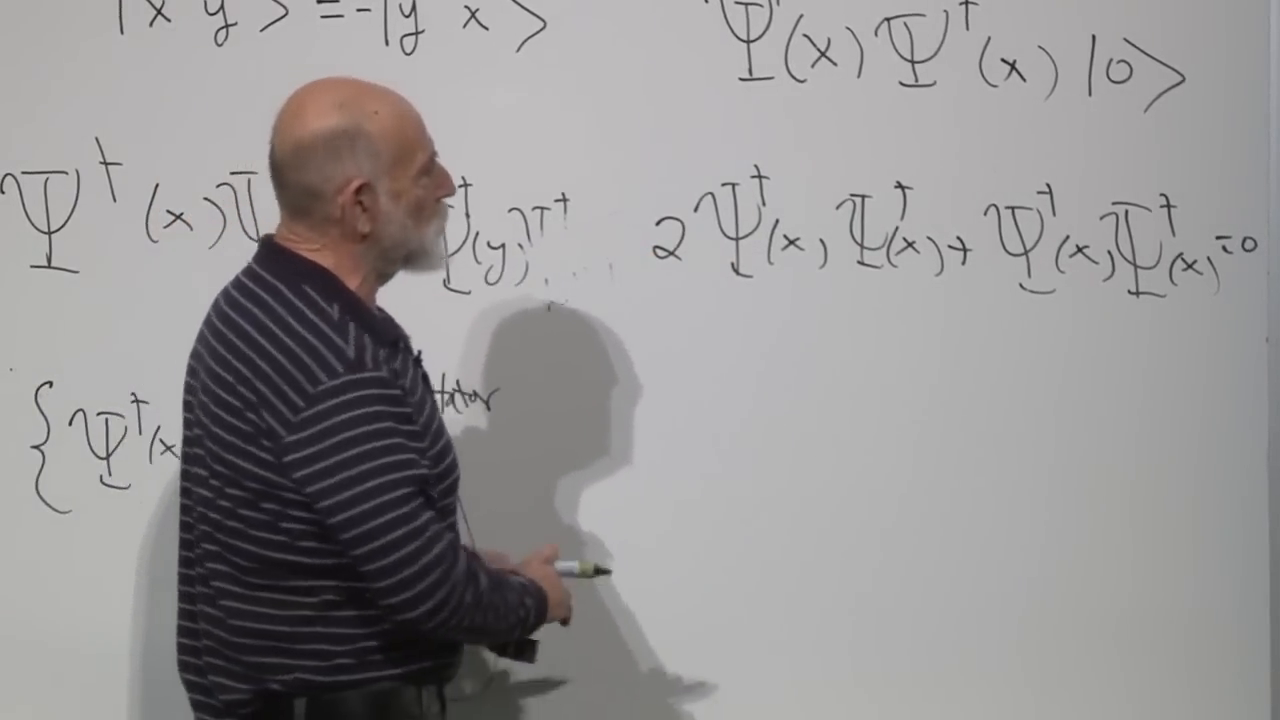
\includegraphics[width=0.94\linewidth]{lecture_10_figure_03.png}
\caption{Der Spezialfall gleicher Zustände an der Tafel. Das wiederholte Produkt der Erzeugungsoperatoren tritt zweimal auf und muss daher verschwinden.}
\lectureframe{00:08:04}
\end{figure}

\begin{figure}[htbp]
\centering
\begin{adjustbox}{max width=\linewidth}
\begin{tikzpicture}[node distance=1.25cm,>=Latex]
\node[draw,rounded corners,align=center,inner sep=7pt] (a)
  {$\{\psi^\dagger(x),\psi^\dagger(x)\}=0$};
\node[draw,rounded corners,align=center,inner sep=7pt,right=of a] (b)
  {$2(\psi^\dagger(x))^2=0$};
\node[draw,rounded corners,align=center,inner sep=7pt,right=of b] (c)
  {$(\psi^\dagger(x))^2=0$};
\draw[->,thick] (a) -- (b);
\draw[->,thick] (b) -- (c);
\end{tikzpicture}
\end{adjustbox}
\caption{Das Ausschlussargument, rekonstruiert ohne die teilweise ausgewischten Zwischenschritte an der Tafel.}
\end{figure}

\section{Warum bei Fermionen besetzt und leer symmetrisch sind}

Zwischen bosonischen und fermionischen Operatoren gibt es einen zweiten Unterschied, der subtiler ist als das Ausschlussprinzip und später wesentlich wird. Für einen einzelnen bosonischen Modus gilt
\begin{equation}
[a,a^\dagger]=1,
\qquad
n=0,1,2,\ldots.
\end{equation}
Beim Vertauschen von \(a\) und \(a^\dagger\) ändert sich das Vorzeichen des Kommutators. Selbst wenn die Operatoren lediglich \(A\) und \(B\) hießen, würde die Algebra verraten, welche Reihenfolge die Besetzungszahl erhöht und welche sie verringert.

Auch die bosonische Besetzungsleiter hat eine Orientierung. Der Vernichtungsoperator erreicht schließlich \(\lvert0\rangle\) und wirkt darauf mit null, während der Erzeugungsoperator unbegrenzt weiterwirken kann:
\begin{align}
a\lvert0\rangle&=0,\\
a^\dagger\lvert n\rangle&\propto\lvert n+1\rangle,
\qquad n=0,1,2,\ldots.
\end{align}
Kehrt man diese Leiter um, erhält man nicht dasselbe Spektrum. Es gibt eine untere Grenze, aber keine obere.

Für einen einzelnen fermionischen Modus gilt
\begin{equation}
\{a,a^\dagger\}=1,
\qquad
a^2=(a^\dagger)^2=0,
\qquad
n=0,1.
\label{eq:l10-fermion-mode}
\end{equation}
Der Erzeugungsoperator überführt den leeren Zustand in den besetzten Zustand und wirkt danach mit null:
\begin{equation}
a^\dagger\lvert0\rangle=\lvert1\rangle,
\qquad
a^\dagger\lvert1\rangle=0.
\end{equation}
Der Vernichtungsoperator bewirkt die Umkehrung:
\begin{equation}
a\lvert1\rangle=\lvert0\rangle,
\qquad
a\lvert0\rangle=0.
\end{equation}
Es gibt nur zwei Zustände. Daher ist das Diagramm unter dem Vertauschen von „besetzt“ und „leer“ sowie von \(a\) und \(a^\dagger\) symmetrisch. Die Operatoren haben weiterhin unterschiedliche physikalische Bedeutungen, doch ihre Algebra zeichnet den einen nicht mehr als Erzeugungsoperator und den anderen als Vernichtungsoperator aus. Diese formale Symmetrie bildet den Ausgangspunkt für die Teilchen-Loch-Umdeutung.

\begin{classroomqa}
\lecturetimestamp{00:13:54}
\audiencequestion{Wenn \((a^\dagger)^2=0\) gilt, ist das ein Widerspruch, oder folgt daraus, dass \(a^\dagger=0\)?}
\lecturerresponse{Weder noch. Ein von null verschiedener Operator kann ein verschwindendes Quadrat haben. Hier überführt \(a^\dagger\) den Zustand \(\lvert0\rangle\) in \(\lvert1\rangle\), doch oberhalb von \(\lvert1\rangle\) gibt es keinen erlaubten Zustand. Zweimalige Anwendung ergibt daher null. Dieselbe Überlegung liefert \(a^2=0\).}
\end{classroomqa}

Behalten wir diese Symmetrie zwischen besetzt und leer im Hinterkopf. Wenn später ein Elektron mit negativer Energie entfernt wird, wird der Vernichtungsoperator als Erzeugungsoperator eines Positrons umgedeutet. Das ist keine willkürliche Änderung der Bezeichnung; sie nutzt genau die hier hergeleitete Zweizustandsalgebra der Fermionen.

\section{Die eindimensionale Dirac-Konstruktion}

Kehren wir nun zu einem Teilchen in einer Raumdimension zurück. Die einfachste relativistische Wellengleichung erster Ordnung lautet
\begin{equation}
i\partial_t\psi=-\,i\partial_x\psi.
\label{eq:l10-right-mover}
\end{equation}
Mit \(P=-i\partial_x\) wird daraus
\begin{equation}
H=P.
\end{equation}
Für einen Impulseigenzustand gilt \(E=p\), und seine Gruppengeschwindigkeit ist
\begin{equation}
v_g=\frac{dE}{dp}=1.
\end{equation}
Sowohl bei positivem als auch bei negativem Impuls und damit bei positiver wie negativer Energie bewegt sich die Welle weiterhin starr nach rechts. Das Vorzeichen von \(p\) ändert das Phasenmuster, nicht die Ausbreitungsrichtung.

Ein massives Teilchen muss sich in beide Richtungen bewegen können. Wir führen eine zweite Komponente ein, die folgende Gleichung erfüllt:
\begin{equation}
H\psi_1=P\psi_1,
\qquad
H\psi_2=-P\psi_2.
\label{eq:l10-two-directions}
\end{equation}
Die erste Komponente bewegt sich nach rechts, die zweite nach links. Wir fassen sie zu einem Spaltenvektor zusammen,
\begin{equation}
\Psi=
\begin{pmatrix}
\psi_1\\
\psi_2
\end{pmatrix},
\end{equation}
und definieren
\begin{equation}
\alpha=
\begin{pmatrix}
1&0\\
0&-1
\end{pmatrix}.
\end{equation}
Damit lassen sich beide Gleichungen schreiben als
\begin{equation}
H\Psi=\alpha P\Psi.
\label{eq:l10-massless-one-d}
\end{equation}
Für die Berücksichtigung beider Richtungen kommt ein neuer zweifachwertiger innerer Freiheitsgrad hinzu.

Die Richtung allein führt noch nicht zur Masse. Wir führen eine zweite Matrix ein,
\begin{equation}
\beta=
\begin{pmatrix}
0&1\\
1&0
\end{pmatrix},
\end{equation}
und setzen an:
\begin{equation}
H=\alpha P+\beta m.
\label{eq:l10-massive-one-d}
\end{equation}
Die Matrizen erfüllen
\begin{equation}
\alpha^2=\beta^2=\mathbb{1},
\qquad
\{\alpha,\beta\}=0.
\label{eq:l10-one-d-algebra}
\end{equation}
Durch Quadrieren des Hamiltonoperators erhalten wir
\begin{align}
H^2
&=(\alpha P+\beta m)^2\\
&=\alpha^2P^2+\beta^2m^2
  +(\alpha\beta+\beta\alpha)Pm\\
&=P^2+m^2.
\label{eq:l10-one-d-dispersion}
\end{align}
Der Antikommutator in Gleichung~\eqref{eq:l10-one-d-algebra} beseitigt den unerwünschten Term, der sowohl von \(P\) als auch von \(m\) linear abhängt.

Die Nebendiagonalmatrix \(\beta\) koppelt die beiden Richtungskomponenten. Man kann sich vorstellen, dass der Massenterm rechts- und linkslaufende Amplituden fortwährend miteinander mischt. Dieses Bild sollte nicht wörtlich als ein Teilchen verstanden werden, das auf einer mikroskopischen Bahn hin und her springt. Es macht jedoch anschaulich, warum ein massives Wellenpaket eine mittlere Geschwindigkeit unterhalb der Lichtgeschwindigkeit haben und ein Ruhesystem besitzen kann, während dies für eine isolierte masselose chirale Komponente nicht möglich ist.

\begin{classroomqa}
\lecturetimestamp{00:23:37}
\audiencequestion{Gibt es eine tiefergehende physikalische Deutung dafür, dass beide Richtungskomponenten eingeführt werden?}
\lecturerresponse{Ja, doch in drei Dimensionen wird sie deutlicher. Hier sind sie zunächst einfach die beiden Komponenten, die nötig sind, um entgegengesetzte Ausbreitungsrichtungen zu beschreiben und eine Massenkopplung über die Nebendiagonale zu ermöglichen. Ihre spätere Deutung lautet Händigkeit oder Chiralität.}
\end{classroomqa}

\section{Drei Dimensionen erzwingen die Pauli-Matrizen}

In drei Raumdimensionen ist der Impuls ein Vektor. Ein in ihm linearer Hamiltonoperator, der ein Rotationsskalar ist, legt daher einen weiteren Vektor nahe, dessen Komponenten nun Matrizen sind:
\begin{equation}
H=\boldsymbol{\alpha}\cdot\mathbf P
=\alpha_xP_x+\alpha_yP_y+\alpha_zP_z.
\label{eq:l10-three-d-ansatz}
\end{equation}

\begin{figure}[htbp]
\centering
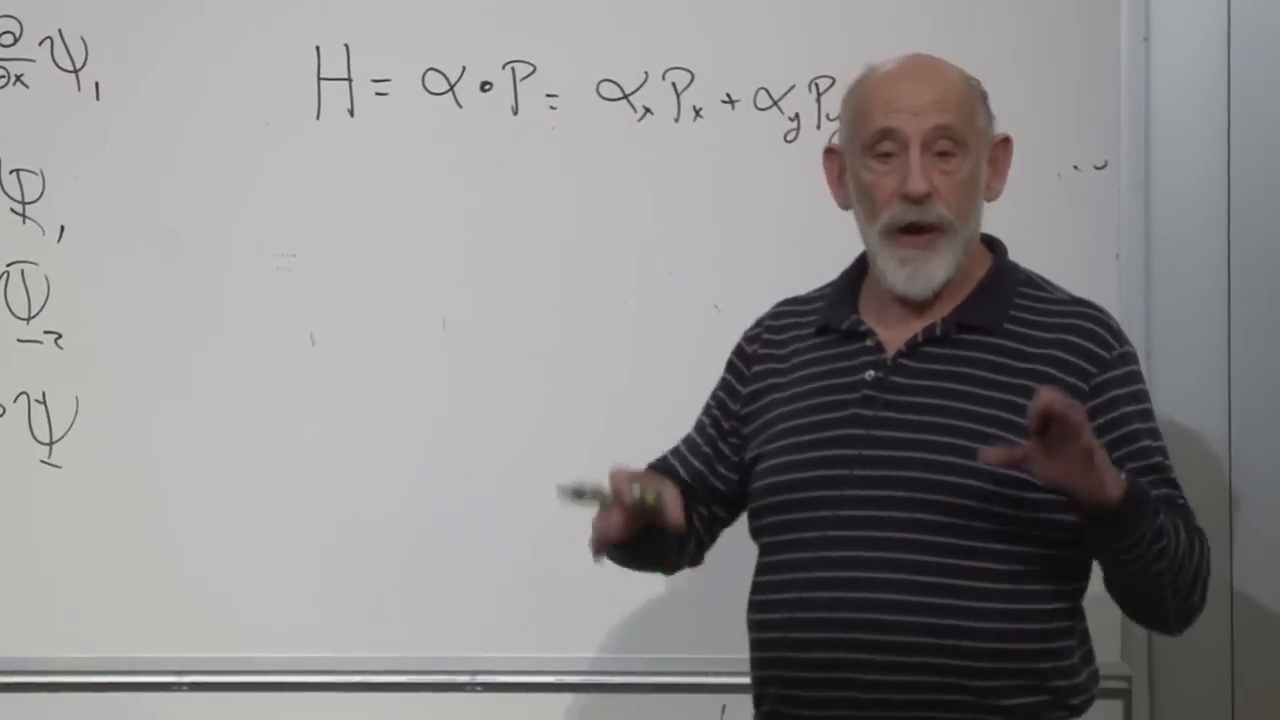
\includegraphics[width=0.94\linewidth]{lecture_10_figure_04.png}
\caption{Der dreidimensionale masselose Ansatz \(H=\boldsymbol{\alpha}\cdot\mathbf P\) an dem Punkt, an dem eine Matrix durch einen Vektor aus drei Matrizen ersetzt wird.}
\lectureframe{00:26:00}
\end{figure}

Beginnen wir erneut mit dem masselosen Fall. Wir verlangen
\begin{equation}
H^2=\mathbf P^2=P_x^2+P_y^2+P_z^2.
\end{equation}
Quadrieren wir Gleichung~\eqref{eq:l10-three-d-ansatz} und entwickeln das Ergebnis,
\begin{align}
H^2
&=\alpha_x^2P_x^2+\alpha_y^2P_y^2\\
&\quad+\alpha_z^2P_z^2\\
&\quad+\{\alpha_x,\alpha_y\}P_xP_y\\
&\quad+\{\alpha_x,\alpha_z\}P_xP_z\\
&\quad+\{\alpha_y,\alpha_z\}P_yP_z.
\end{align}
so stimmen die Diagonalterme, wenn
\begin{equation}
\alpha_x^2=\alpha_y^2=\alpha_z^2=\mathbb{1},
\end{equation}
gilt, und sämtliche Kreuzterme verschwinden, wenn
\begin{equation}
\{\alpha_i,\alpha_j\}=0,
\qquad i\ne j.
\label{eq:l10-alpha-anticommutation}
\end{equation} gilt.

Drei bekannte \(2\times2\)-Matrizen erfüllen genau diese Bedingungen:
\begin{equation}
\sigma_x=
\begin{pmatrix}
0&1\\
1&0
\end{pmatrix},
\quad
\sigma_y=
\begin{pmatrix}
0&-i\\
i&0
\end{pmatrix},
\quad
\sigma_z=
\begin{pmatrix}
1&0\\
0&-1
\end{pmatrix}.
\label{eq:l10-pauli-matrices}
\end{equation}
Eine Lösung lautet also
\begin{equation}
\alpha_i=\sigma_i,
\qquad
H=\boldsymbol{\sigma}\cdot\mathbf P.
\label{eq:l10-weyl-hamiltonian}
\end{equation}

\begin{figure}[htbp]
\centering
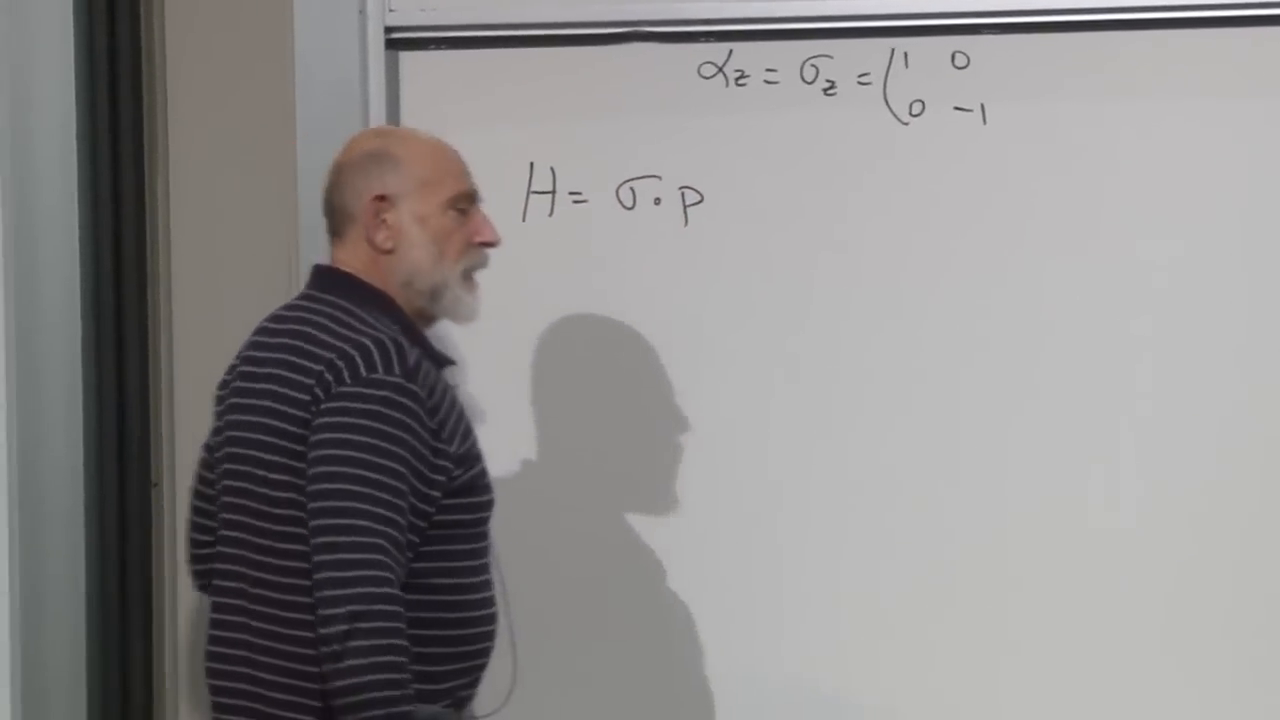
\includegraphics[width=0.94\linewidth]{lecture_10_figure_05.png}
\caption{Der kompakte masselose Hamiltonoperator \(H=\boldsymbol{\sigma}\cdot\mathbf P\), mit dem darüber weiterhin sichtbaren \(\alpha_z=\sigma_z\).}
\lectureframe{00:28:16}
\end{figure}

Für einen Impulseigenzustand gilt
\begin{equation}
\boldsymbol{\sigma}\cdot\mathbf p
=
|\mathbf p|\,\boldsymbol{\sigma}\cdot\widehat{\mathbf p}.
\end{equation}
Der Operator \(\boldsymbol{\sigma}\cdot\widehat{\mathbf p}\) hat die Eigenwerte \(+1\) und \(-1\). Daher gilt
\begin{equation}
E=\pm|\mathbf p|.
\end{equation}
In dieser Zweikomponententheorie ist bei positiver Energie der Pauli-Freiheitsgrad am Impuls ausgerichtet, bei negativer Energie dagegen entgegengesetzt zu ihm. Diese Ausrichtung ist festgelegt; bei gegebenem Vorzeichen der Energie lässt sich die Spinrichtung nicht unabhängig davon wählen.

\begin{classroomqa}
\lecturetimestamp{00:30:10}
\audiencequestion{Ergibt sich der Spin aus der Dirac-Gleichung, oder wurde er eingeführt, weil bereits bekannt war, dass das Elektron ein magnetisches Moment hat?}
\lecturerresponse{Hier bedeutet „sich ergeben“: „als Folge hervorgehen“, nicht „verschwinden“. Ausgangspunkt war die Forderung nach einem in den Impulskomponenten linearen Hamiltonoperator, dessen Quadrat \(\mathbf P^2\) ist. Gewöhnliche Zahlen können die verlangte Algebra nicht erfüllen, die Pauli-Matrizen hingegen schon. Ihre Zweikomponentenstruktur ergibt sich daher bereits aus der Linearisierung selbst. Das beweist nicht, dass jedes Teilchen Spin haben muss; es besagt, dass Teilchen, die durch diese Dirac-artige Gleichung beschrieben werden, den entsprechenden Spinor-Freiheitsgrad besitzen.}
\end{classroomqa}

Dies ist eine der zentralen Lehren dieser Konstruktion. Die Matrizen sind keine dekorativen Bezeichnungen, die nachträglich zur relativistischen Gleichung hinzugefügt werden. Sie entstehen beim Versuch, eine lokale Quadratwurzel der relativistischen Dispersionsrelation zu bilden.

\section{Warum die Masse vier Komponenten erfordert}

Versuchen wir, die eindimensionale Massenkonstruktion zu wiederholen, ohne die \(2\times2\)-Theorie zu erweitern:
\begin{equation}
H=\boldsymbol{\sigma}\cdot\mathbf P+\beta m.
\label{eq:l10-failed-mass}
\end{equation}
Wir nehmen \(\beta^2=\mathbb{1}\) an. Das Quadrat enthält zwar die gewünschten Terme \(\mathbf P^2+m^2\), aber auch
\begin{equation}
m\sum_i\{\sigma_i,\beta\}P_i.
\end{equation}
Um diesen Term zu beseitigen, müsste eine Matrix \(\beta\) die Bedingung
\begin{equation}
\{\sigma_x,\beta\}
=
\{\sigma_y,\beta\}
=
\{\sigma_z,\beta\}
=0.
\label{eq:l10-impossible-beta}
\end{equation}
erfüllen. Es gibt keine Matrix der Größe \(2\times2\) mit dieser Eigenschaft. Die Einheitsmatrix kommutiert mit allen drei Pauli-Matrizen, und jede spurlose Matrix der Größe \(2\times2\) ist eine Linearkombination der Pauli-Matrizen. Jede solche Kombination antikommutiert nicht mit der Komponente, die parallel zu ihr ist. In der \(2\times2\)-Algebra gibt es keine vierte unabhängige Matrix der benötigten Art.

Abhilfe schafft eine Erweiterung des Spinors. Vier Matrizen, die paarweise antikommutieren und deren Quadrate die Einheitsmatrix sind, treten erstmals in einer komplexen Darstellung der Größe \(4\times4\) auf. Diese Matrixgröße wurde nicht deshalb gewählt, weil die Raumzeit vier Dimensionen hat; sie ist der kleinste Matrizenraum, in dem sich die geforderte Algebra realisieren lässt.

Es gibt viele äquivalente Darstellungen. Eine unitäre Änderung der Spinorbasis verändert die Einträge sämtlicher Matrizen, ohne eine physikalische Vorhersage zu ändern. Entscheidend ist die abstrakte Menge der Relationen
\begin{equation}
\{\alpha_i,\alpha_j\}=2\delta_{ij}\mathbb{1},
\qquad
\{\alpha_i,\beta\}=0,
\qquad
\beta^2=\mathbb{1}.
\label{eq:l10-dirac-algebra}
\end{equation}

\begin{classroomqa}
\lecturetimestamp{00:37:38}
\audiencequestion{Kann man \(\beta\) als Zeitkomponente \(\alpha_t\) auffassen?}
\lecturerresponse{Nicht unmittelbar. Die drei \(\alpha_i\) bilden mit \(\beta\) nicht die vier Komponenten eines einzigen Lorentz-Vektors. In kovarianter Notation definiert man stattdessen \(\beta=\gamma^0\) und \(\alpha_i=\gamma^0\gamma^i\); die vier Matrizen \(\gamma^\mu\) erfüllen die Raumzeit-Clifford-Algebra.}
\end{classroomqa}

Eine praktische Blockdarstellung ist
\begin{equation}
\alpha_i=
\begin{pmatrix}
\sigma_i&0\\
0&-\sigma_i
\end{pmatrix},
\qquad
\beta=
\begin{pmatrix}
0&I_2\\
I_2&0
\end{pmatrix}.
\label{eq:l10-block-representation}
\end{equation}
Die Pauli-Matrizen in den Diagonalblöcken gewährleisten, dass verschiedene \(\alpha_i\) antikommutieren. Die Einheitsmatrizen in den Nebendiagonalblöcken von \(\beta\) gewährleisten, dass \(\beta\) mit jedem \(\alpha_i\) antikommutiert.

\begin{figure}[htbp]
\centering
\includegraphics[width=0.94\linewidth]{lecture_10_figure_06.png}
\caption{Die Blockdarstellung der Größe \(4\times4\) an der Tafel. Die oberen Gleichungen geben die geforderten Antikommutatoren an; die vollständigen Matrizen sind in Gleichung~\eqref{eq:l10-block-representation} gesetzt.}
\lectureframe{00:41:10}
\end{figure}

Der massive Hamiltonoperator lautet nun
\begin{equation}
H=\boldsymbol{\alpha}\cdot\mathbf P+\beta m
=
\begin{pmatrix}
\boldsymbol{\sigma}\cdot\mathbf P&mI_2\\
mI_2&-\boldsymbol{\sigma}\cdot\mathbf P
\end{pmatrix}.
\label{eq:l10-massive-dirac}
\end{equation}
Unter Verwendung von Gleichung~\eqref{eq:l10-dirac-algebra} erhalten wir
\begin{equation}
H^2=\mathbf P^2+m^2.
\end{equation}
Die Vierkomponentenstruktur ist also keine optionale Ergänzung. Sie ist die kleinste Struktur, die sowohl einen dreidimensionalen Impuls als auch einen Massenterm zulässt und zugleich die Gleichung erster Ordnung erhält.

\section{Chiralität und die Bedeutung der zusätzlichen Komponenten}

Welche physikalische Unterscheidung kommt durch die Erweiterung hinzu? Betrachten wir zunächst den masselosen oberen Block,
\begin{equation}
H_R=\boldsymbol{\sigma}\cdot\mathbf P,
\end{equation}
und den masselosen unteren Block,
\begin{equation}
H_L=-\boldsymbol{\sigma}\cdot\mathbf P.
\end{equation}
Bei Zuständen mit positiver Energie ist im ersten Block der Spin am Impuls ausgerichtet, im zweiten dagegen entgegengesetzt. Es handelt sich um entgegengesetzte Helizitäten. In einer masselosen Theorie bleibt die Helizität unter eigentlichen Lorentz-Transformationen invariant, denn kein Beobachter kann ein lichtartiges Teilchen überholen und dessen Impuls umkehren, während sein Spin unverändert bleibt. Die beiden Blöcke beschreiben daher entgegengesetzte chirale Sektoren.

\begin{classroomqa}
\lecturetimestamp{00:41:28}
\audiencequestion{In einer Dimension war ein zusätzlicher binärer Freiheitsgrad nötig, um Masse einzuführen. Welche physikalische Unterscheidung entspricht ihm in drei Dimensionen?}
\lecturerresponse{Es ist die Händigkeit des Spinors. Die beiden Blöcke der Größe \(2\times2\) beschreiben entgegengesetzte Beziehungen zwischen Spin und Impuls. Der eine ist rechtshändig, der andere linkshändig. Die Theorie mit Matrizen der Größe \(4\times4\) umfasst beide.}
\end{classroomqa}

Der Massenterm in Gleichung~\eqref{eq:l10-massive-dirac} steht außerhalb der Diagonale. Er überführt eine Amplitude des oberen Blocks in den unteren Block und umgekehrt:
\begin{equation}
\beta m
\begin{pmatrix}
\Psi_R\\
\Psi_L
\end{pmatrix}
=
m
\begin{pmatrix}
\Psi_L\\
\Psi_R
\end{pmatrix}.
\end{equation}
Masse koppelt also entgegengesetzte Chiralitäten miteinander.

\begin{classroomqa}
\lecturetimestamp{00:43:58}
\audiencequestion{Kann ein masseloses Teilchen seine Chiralität ändern?}
\lecturerresponse{Nicht unter dem hier gezeigten freien masselosen Hamiltonoperator. Die beiden Blöcke sind entkoppelt, sodass ein anfangs rechts- oder linkshändiger Zustand dies auch bleibt. Genau der Nebendiagonalterm für die Masse mischt die beiden, wenn \(m\ne0\) gilt.}
\end{classroomqa}

Diese Aussage ist für die Blockdarstellung exakt. Das Bild eines Teilchens, das mechanisch zwischen zwei Pfeilen hin- und herwechselt, sollte man jedoch nicht überstrapazieren. Die physikalische Aussage ist die Matrixkopplung in der Wellengleichung.

\begin{classroomqa}
\lecturetimestamp{00:44:50}
\audiencequestion{Sind diese Matrizen in den Quaternionen angelegt?}
\lecturerresponse{Die Pauli-Matrizen stehen in engem Zusammenhang mit den Quaternioneneinheiten: Die Matrizen \(-i\sigma_i\) haben das Quadrat \(-\mathbb{1}\) und multiplizieren sich bis auf Konventionen für die Orientierung nach dem quaternionischen Muster. Die vollständigen Dirac-Matrizen erfordern die größere Clifford-Algebra. Für das folgende Argument wird der Zusammenhang mit den Quaternionen nicht benötigt.}
\end{classroomqa}

\begin{classroomqa}
\lecturetimestamp{00:46:34}
\audiencequestion{Wenn Spin Drehimpuls ist, gibt es hier dann einen eigenen Energiebeitrag, der ihm zugeordnet ist?}
\lecturerresponse{Es wird kein unabhängiger Term für ein freies Teilchen hinzugefügt. Die Spinorstruktur geht bereits über die Matrizen in den kinetischen Hamiltonoperator ein. Die Kopplung des Spins an ein äußeres Magnetfeld würde zusätzliche Wechselwirkungsterme einführen, doch das ist ein anderes Problem.}
\end{classroomqa}

\section{Die Alpha-Matrizen stehen für die Geschwindigkeit, nicht für den Spin}

Jede \(\alpha_i\) hat je zwei Eigenwerte \(+1\) und \(-1\). Verschiedene Komponenten kommutieren nicht miteinander, sodass sie nicht alle gleichzeitig scharf gemessen werden können. Um die Bedeutung einer einzelnen Komponente zu bestimmen, verwenden wir die Heisenberg-Gleichung. Für einen Operator \(L\) ohne explizite Zeitabhängigkeit gilt
\begin{equation}
\dot L=i[H,L].
\label{eq:l10-heisenberg}
\end{equation}
Die Vorzeichenkonvention ist hier durch die Schr\"odinger-Entwicklung \(e^{-iHt}\) festgelegt.

Wenden wir Gleichung~\eqref{eq:l10-heisenberg} auf den Ortsoperator \(x\) an. Die Matrizen wirken auf Spinorindizes und kommutieren mit dem Ort. Nur \(P_x\) kommutiert nicht mit \(x\):
\begin{align}
\dot x
&=i[\boldsymbol{\alpha}\cdot\mathbf P+\beta m,x]\\
&=i\alpha_x[P_x,x]\\
&=\alpha_x,
\label{eq:l10-velocity}
\end{align}
da \([P_x,x]=-i\) gilt. Somit ist \(\alpha_x\) die \(x\)-Komponente des Geschwindigkeitsoperators; entsprechend gilt
\begin{equation}
\dot{\mathbf x}=\boldsymbol{\alpha}.
\end{equation}

\begin{classroomqa}
\lecturetimestamp{00:51:50}
\audiencequestion{Ergibt eine Messung einer Geschwindigkeitskomponente tatsächlich nur \(+1\) oder \(-1\)?}
\lecturerresponse{Ja, für den momentanen Operator \(\alpha_i\) in Einheiten mit \(c=1\). Ein allgemeiner Zustand muss kein Eigenzustand sein, daher kann sein Erwartungswert jeden Wert zwischen diesen beiden annehmen. Das gleichmäßig fortbewegte Wellenpaket hat bei einem massiven Teilchen eine mittlere Geschwindigkeit unterhalb der Lichtgeschwindigkeit.}
\end{classroomqa}

Die Geschwindigkeit ist keine Erhaltungsgröße:
\begin{equation}
\dot\alpha_x=i[H,\alpha_x]\ne0.
\end{equation}
Die Terme mit \(\alpha_y\), \(\alpha_z\) und \(\beta\) kommutieren nicht mit \(\alpha_x\). Ein Zustand mit positiven und negativen Energiekomponenten weist daher einen rasch oszillierenden Beitrag zu seinem Ort auf. Das ist \emph{Zitterbewegung}, wörtlich eine zitternde Bewegung.

Mittelt man über Zeiträume, die lang gegenüber der raschen Oszillation sind, ergibt sich für die relativistische Geschwindigkeit
\begin{equation}
\overline{\mathbf v}=\frac{\mathbf p}{E},
\end{equation}
Für ein langsames Elektron geht dies in \(\mathbf p/m\) über.

\begin{classroomqa}
\lecturetimestamp{00:54:40}
\audiencequestion{Verletzt ein freies Elektron, das ohne äußere Kraft zittert, Newtons Gesetz?}
\lecturerresponse{Nein. Aufgrund der Translationsinvarianz bleibt der Impuls erhalten, also gilt \(\dot{\mathbf P}=0\). Der Dirac-Geschwindigkeitsoperator ist nicht einfach \(\mathbf P/m\), und sein rasch oszillierender Anteil kann sich ändern, während der Impuls konstant bleibt. Die zeitlich gemittelte Bewegung folgt der erwarteten Beziehung für ein freies Teilchen.}
\end{classroomqa}

\begin{classroomqa}
\lecturetimestamp{00:55:22}
\audiencequestion{Ist die Geschwindigkeit immer \(c\)?}
\lecturerresponse{Eine momentane Messung einer Komponente \(\alpha_i\) hat die Eigenwerte \(\pm c\). Ein massives Wellenpaket ist jedoch im Allgemeinen eine Überlagerung und hat einen Erwartungswert unterhalb der Lichtgeschwindigkeit. Seine mittlere Gruppengeschwindigkeit ist \(\mathbf p/E\).}
\end{classroomqa}

\begin{classroomqa}
\lecturetimestamp{00:55:30}
\audiencequestion{Kann man sich die Oszillation so vorstellen, dass die Masse die Geschwindigkeit verändert?}
\lecturerresponse{Nein. Die Masse ist ein fester Parameter. Die Oszillation entsteht durch nichtkommutierende Geschwindigkeits- und Hamiltonoperatoren oder, gleichbedeutend, durch Interferenz zwischen Energiesektoren, nicht durch eine schwankende Masse.}
\end{classroomqa}

\begin{classroomqa}
\lecturetimestamp{00:56:22}
\audiencequestion{Kann eine momentane Messung eine Geschwindigkeit in eine Richtung ergeben, obwohl die mittlere Bewegung in eine andere Richtung weist?}
\lecturerresponse{Ja. Die Komponentenoperatoren haben die beiden scharfen Eigenwerte, während wiederholte oder zeitlich gemittelte Messungen die gleichmäßigere Drift ergeben.}
\end{classroomqa}

Auch der Begriff Spin muss mit Bedacht verwendet werden. Die \(\alpha_i\) transformieren sich wie die Komponenten der Geschwindigkeit, also wie ein gewöhnlicher Vektor. Der eigentliche Spinoperator in dieser Darstellung ist
\begin{equation}
\mathbf S=\frac12\boldsymbol{\Sigma},
\qquad
\Sigma_i=
\begin{pmatrix}
\sigma_i&0\\
0&\sigma_i
\end{pmatrix}.
\label{eq:l10-spin-operator}
\end{equation}
Er unterscheidet sich von \(\alpha_i\) durch das Vorzeichen des unteren Blocks. Die Matrizen hängen zwar eng zusammen, doch Geschwindigkeit und Spin sind nicht dieselbe Observable.

\section{Negative Energie und das Vakuum niedrigster Energie}

Das Problem der negativen Energie besteht bereits, bevor wir diese gesamte Matrixtechnik einführen. Kehren wir zum eindimensionalen Rechtspfeil zurück:
\begin{equation}
H=P.
\end{equation}
Da \(p\) die gesamte reelle Achse durchläuft, ist \(E=p\) nach unten unbeschränkt.

Das Vakuum kann nicht einfach ein Zustand ohne Teilchen sein. Es muss ein Zustand sein, dem sich keine weitere Energie entziehen lässt. Wenn wir aus einem leeren Zustand ein Teilchen mit negativer Energie hinzufügen, dadurch die Energie verringern, ein weiteres hinzufügen und unbegrenzt so fortfahren können, ist dieser leere Zustand kein stabiles Vakuum.

Die Fermi-Statistik bietet einen historisch bedeutsamen Ausweg. Wir setzen ein Elektron in jeden Zustand negativer Energie. Jedes hinzugefügte Elektron senkt die Gesamtenergie, doch aufgrund des Ausschlussprinzips kann jeder Einteilchenzustand nur ein Elektron besetzen. Sobald alle Zustände negativer Energie gefüllt sind, kann kein weiteres Elektron in diesen Sektor fallen. Dirac identifizierte diese vollständig besetzte Konfiguration als das Vakuum.

Bei Bosonen würde dieselbe Konstruktion scheitern. Beliebig viele Bosonen können denselben Zustand besetzen. Ein bosonischer Modus negativer Energie könnte daher unbegrenzt Teilchen aufnehmen. Die fermionische Schranke \(n=0,1\), die zu Beginn der Vorlesung eingeführt wurde, verhindert genau diesen Energieabstieg.

\begin{figure}[htbp]
\centering
\includegraphics[width=0.94\linewidth]{lecture_10_figure_07.png}
\caption{Das historische Bild des Dirac-Meers an der Tafel: eine Leiter negativer Energieniveaus, die bis zur Trennlinie besetzt sind, mit Zuständen positiver Energie darüber.}
\lectureframe{01:02:45}
\end{figure}

\begin{figure}[htbp]
\centering
\begin{adjustbox}{max width=\linewidth}
\begin{tikzpicture}[x=1.05cm,y=0.72cm,>=Latex]
\draw[->] (0,-4.8) -- (0,4.8) node[above] {$E$};
\draw[thick] (-2.9,0) -- (3.2,0) node[right] {$E=0$};
\foreach \y in {-4,-3.3,...,-0.5} {
  \draw (-2.3,\y) -- (2.3,\y);
  \foreach \x in {-1.8,-1.2,...,1.8} {
    \fill[blue!65!black] (\x,\y) circle (1.6pt);
  }
}
\foreach \y in {0.8,1.6,...,4.0} {
  \draw (-2.3,\y) -- (2.3,\y);
}
\draw[red,very thick] (0.6,-2.6) circle (5pt);
\draw[red,->,very thick] (0.6,-2.35) .. controls (1.4,-0.4) and (1.2,1.6) .. (1.5,2.4);
\fill[red] (1.5,2.4) circle (2.5pt);
\node[right,red] at (0.85,-2.6) {hole};
\node[right,red] at (1.7,2.4) {$e^-$};
\node[left] at (-2.5,-2.2) {filled negative-energy states};
\end{tikzpicture}
\end{adjustbox}
\caption{Eine saubere Rekonstruktion einer Anregung über dem gefüllten Meer: Hebt man ein Elektron negativer Energie an, bleibt ein Loch positiver Energie zurück.}
\end{figure}

Das Bild vom Meer ist eine historische Ausdrucksweise für eine korrekte Umordnung der Operatoren. Seine wörtlich verstandene unendliche Ladung und Energie dürfen nicht mit unmittelbar beobachtbaren Größen verwechselt werden; die moderne Neuformulierung macht es überflüssig, sich materielle Elektronen vorzustellen, die den Raum ausfüllen.

\section{Ein Loch ist ein Positron}

Sind alle Zustände negativer Energie besetzt, sind zwei Arten von Anregungen möglich. Wir können ein Elektron positiver Energie oberhalb des Meers hinzufügen. Oder wir können ein Elektron negativer Energie entfernen und ein Loch zurücklassen.

Ein Loch hat die entgegengesetzte Ladung des fehlenden Elektrons. Entfernt man die Ladung \(-e\), ändert sich die Ladung um \(+e\). Das Loch hat außerdem eine positive Anregungsenergie. Hatte das entfernte Elektron die Energie \(E_-<0\), so ändert sich die Energie, gemessen relativ zum gefüllten Vakuum, um
\begin{equation}
E_{\mathrm{hole}}=-E_->0.
\end{equation}
Das Loch ist eine positiv geladene Anregung mit positiver Energie: das Positron.

Ein Photon kann ein Elektron aus dem Meer in einen Zustand positiver Energie anheben. Relativ zum Vakuum enthält der Endzustand dann ein Elektron und ein Positron. In einem zeitgeordneten Diagramm zeichnet man den Elektronenzahlfluss für das Elektron konventionell nach oben und die Positronenlinie mit dem entgegengesetzten Pfeil. Die Pfeile kennzeichnen den Fluss der Fermionenzahl oder der Ladung; sie sind keine kleinen klassischen Geschwindigkeitsvektoren.

\begin{classroomqa}
\lecturetimestamp{01:05:14}
\audiencequestion{Müssen in diesem Bild gleich viele Elektronen und Positronen vorkommen?}
\lecturerresponse{Nicht in einem beliebigen Zustand. Beginnt man beim Vakuum und erzeugt ein neutrales Paar, erhält man je ein Teilchen. Ein Zustand kann jedoch bereits einen Überschuss an Elektronen oder Positronen enthalten. Die Ladungserhaltung schränkt Reaktionen ein; sie verlangt nicht, dass jeder erlaubte Zustand gleich viele Teilchen beider Arten enthält.}
\end{classroomqa}

Dirac wusste zunächst nicht, dass das Loch ein Teilchen sein würde, das dieselbe Masse wie das Elektron und nur eine entgegengesetzte Ladung sowie andere additive Quantenzahlen hat. Die Gleichung und die Lochkonstruktion führten zu dieser Vorhersage, noch bevor das Positron in den vertrauten Teilchenkatalog aufgenommen wurde.

\section{Ein einziges Fermionenfeld enthält Elektronen und Positronen}

Der Feldoperator überführt das historische Bild in die moderne Algebra. Für den Moment lassen wir Spinorindizes, Normierungsfaktoren und die Zeitabhängigkeit weg. Ein eindimensionales Feld lässt sich schematisch entwickeln als
\begin{equation}
\psi(x)
\sim
\int_{-\infty}^{\infty}dp\,a(p)e^{ipx}.
\label{eq:l10-full-field-integral}
\end{equation}
Für die Dispersion eines Rechtspfeils \(E=p\) kennzeichnet positives \(p\) positive Energie und negatives \(p\) negative Energie. Wir teilen das Integral auf:
\begin{equation}
\psi(x)
\sim
\int_0^\infty dp\,a(p)e^{ipx}
+
\int_{-\infty}^0 dp\,a(p)e^{ipx}.
\end{equation}
Im zweiten Term setzen wir \(p=-q\) mit \(q>0\) und deuten die Vernichtung eines besetzten Elektrons negativer Energie als Erzeugung eines Positrons um:
\begin{equation}
b^\dagger(q):=a(-q).
\end{equation}
Dann gilt
\begin{equation}
\psi(x)
\sim
\int_0^\infty dp\,
\left[
a(p)e^{ipx}
+
b^\dagger(p)e^{-ipx}
\right].
\label{eq:l10-electron-positron-split}
\end{equation}
Die genauen Vorzeichen der ebenen Wellenphasen hängen von der Raumzeitkonvention ab; der invariante Inhalt ist, dass \(\psi\) einen Elektronenvernichtungsoperator und einen Positonenerzeugungsoperator enthält.

\begin{figure}[htbp]
\centering
\includegraphics[width=0.94\linewidth]{lecture_10_figure_08.png}
\caption{Das Feldintegral, aufgeteilt in Sektoren positiver und negativer Energie. In der unteren Zeile wird der Operator des Elektrons negativer Energie als Positonenerzeugungsoperator umgedeutet.}
\lectureframe{01:11:35}
\end{figure}

Hier zahlt sich die Symmetrie zwischen besetzt und leer aus Gleichung~\eqref{eq:l10-fermion-mode} aus. Bei Fermionen erlaubt die Operatoralgebra diese Umdeutung, ohne die Antikommutationsstruktur zu verändern.

Eine schematische elektromagnetische Wechselwirkung hat die Form
\begin{equation}
H_{\mathrm{int}}
\sim
\int dx\,\psi^\dagger(x)\psi(x)A(x),
\label{eq:l10-qed-schematic}
\end{equation}
Dabei bezeichnet \(A\) das Photonenfeld. Da jedes Fermionenfeld Anteile von Elektronen und Positronen enthält, umfasst ein einzelner lokaler Operator mehrere Reaktionskanäle:
\begin{align}
e^-&\longrightarrow e^-+\gamma,\\
e^-+e^+&\longrightarrow\gamma,\\
\gamma&\longrightarrow e^-+e^+,
\end{align}
sowie die dazu inversen und gekreuzten Prozesse. Die Energie-Impuls-Erhaltung entscheidet, welcher Kanal in einer bestimmten Umgebung kinematisch möglich ist. Ein isoliertes reales Photon im Vakuum kann beispielsweise kein Paar erzeugen, solange kein weiterer Beteiligter den Rückstoß aufnimmt, auch wenn der lokale Vertex in der Wechselwirkung vorhanden ist.

\begin{figure}[htbp]
\centering
\includegraphics[width=0.94\linewidth]{lecture_10_figure_09.png}
\caption{Die Tafel stellt die Elektronenemission, die Paarvernichtung und die schematische Wechselwirkung \(\psi^\dagger\psi A\) nebeneinander. Unterschiedliche Auswahlmöglichkeiten bei denselben Feldoperatoren erzeugen die verschiedenen Reaktionskanäle.}
\lectureframe{01:13:30}
\end{figure}

Ein einziges kompaktes Produkt von Feldern ordnet somit viele scheinbar unterschiedliche Reaktionen. Feynman entwickelte später die systematischen diagrammatischen Regeln zur Berechnung der Amplituden, doch ein großer Teil der Operatorstruktur ist bereits hier zu erkennen.

\section{Die moderne Sprache für das Vakuum und die Analogie zum Fermisee}

\begin{classroomqa}
\lecturetimestamp{01:14:20}
\audiencequestion{Wie beschreiben Physikerinnen und Physiker das heute, ohne das Vakuum als wörtliches Dirac-Meer aufzufassen?}
\lecturerresponse{Sie nehmen die Umdeutung direkt auf der Ebene der Operatoren vor. Die Vernichtung eines Elektrons negativer Energie wird in die Erzeugung eines Positrons positiver Energie umbenannt. Das Vakuum wird als der Zustand definiert, der von allen Vernichtungsoperatoren für Elektronen und Positronen vernichtet wird. Die resultierende Formulierung ist symmetrisch bezüglich Teilchen und Antiteilchen und benötigt kein materielles Meer.}
\end{classroomqa}

Die historische Dirac-See bleibt nützlich, weil ihre Logik eine enge Entsprechung in der Festkörperphysik hat. In einem Kristall besetzen eine feste Anzahl von Elektronen die niedrigsten verfügbaren Einteilchenzustände bis zur Fermi-Energie. Der gefüllte Grundzustand ist nicht leer. Wird ein Elektron über diese Energie gehoben, bleibt darunter ein unbesetzter Zustand zurück. Relativ zum gefüllten Hintergrund trägt das Loch eine positive Anregungsenergie und kann sich wie ein positiver Ladungsträger verhalten.

Es gibt wichtige Unterschiede. Ein Loch in einem Festkörper befindet sich in einem Medium; seine effektive Masse und seine Reaktion auf elektrische Ladung hängen von der Bandstruktur ab. Ein Positron ist ein elementares Antiteilchen im relativistischen Quantenfeld. Dennoch macht die gemeinsame Teilchen-Loch-Algebra die Analogie sehr leistungsfähig.

\begin{classroomqa}
\lecturetimestamp{01:17:14}
\audiencequestion{Leidet die Klein--Gordon-Theorie für Bosonen unter demselben Kaskadeneffekt hin zu Zuständen negativer Energie?}
\lecturerresponse{Nein. Ein korrekt quantisiertes komplexes Klein--Gordon-Feld ist in Teilchen und Antiteilchen positiver Energie gegliedert, ohne dass eine bosonische See gefüllt werden müsste. Seine Differentialgleichung zweiter Ordnung und seine kanonische Struktur unterscheiden sich von der Konstruktion des Dirac-Hamiltonoperators; deshalb lässt sich das historische Argument der fermionischen See nicht unverändert übertragen.}
\end{classroomqa}

\begin{classroomqa}
\lecturetimestamp{01:17:30}
\audiencequestion{Woher kommt der Spin eins bei Bosonen?}
\lecturerresponse{Nicht aus der hier verwendeten Linearisierung mit Pauli-Matrizen. Felder mit Spin eins haben ihr eigenes Lorentz-Transformationsgesetz und eigene Feldgleichungen. Die vorliegende Herleitung erklärt die Spinorstruktur der Dirac-Fermionen, nicht alle möglichen Teilchenspins.}
\end{classroomqa}

\begin{classroomqa}
\lecturetimestamp{01:17:46}
\audiencequestion{Warum war die Fermi-Statistik für die Lösung negativer Energie wesentlich?}
\lecturerresponse{Weil das Pauli-Prinzip die Besetzung jedes Zustands auf ein Elektron begrenzt. Sobald alle Zustände negativer Energie besetzt sind, kann kein weiteres Elektron in sie hinabfallen. Für bosonische Besetzungszahlen gibt es keine solche Obergrenze; eine wörtlich verstandene See negativer Energie für Bosonen hätte daher weiterhin keinen unteren Grenzzustand.}
\end{classroomqa}

\begin{classroomqa}
\lecturetimestamp{01:20:02}
\audiencequestion{Ist der Unterschied zwischen Elektron und Positron einfach ein weiterer binärer Freiheitsgrad, ähnlich der Ladung?}
\lecturerresponse{Für die Zustandszählung hat ein massives Dirac-Feld zwei Elektronenspinzustände und zwei Positronenspinzustände; daher sind zwei binäre Kennzeichnungen eine nützliche Merkhilfe. Teilchen und Antiteilchen sind jedoch keine unabhängig drehbaren inneren Qubits eines einzelnen Elektrons: Jedes Elektron trägt die Ladung \(-e\), jedes Positron die Ladung \(+e\), und die Unterscheidung ergibt sich nach der Quantisierung aus den Sektoren positiver und negativer Frequenzen.}
\end{classroomqa}

Die unendliche See wirft noch eine letzte Frage auf.

\begin{classroomqa}
\lecturetimestamp{01:20:54}
\audiencequestion{Würde die unendliche Dirac-See zu einer unendlichen kosmologischen Konstante führen?}
\lecturerresponse{Sie macht das Problem der Vakuumenergie sichtbar. Bosonische Nullpunktsmoden tragen \(+\tfrac12\hbar\omega\) bei, während fermionische Moden mit umgekehrtem Vorzeichen beitragen. Formale Auslöschungen sind möglich, wenn die Spektren übereinstimmen; die Spektren von Elektron und Photon stimmen jedoch nicht überein, sodass ein enormer Rest zu erwarten ist. Ohne Gravitation kann eine konstante Verschiebung des Hamiltonoperators abgezogen werden, weil nur Energiedifferenzen von Bedeutung sind. Mit Gravitation wirkt die absolute Vakuumenergie gravitativ; dadurch wird die Subtraktion zu einem physikalischen Problem und nicht zu einer bloßen Frage der Buchführung.}
\end{classroomqa}

Zum Schluss kehren wir zur Bedeutung der Masse zurück.

\begin{classroomqa}
\lecturetimestamp{01:22:56}
\audiencequestion{Können wir genauer sagen, wie die Masse linke und rechte Komponenten miteinander verknüpft?}
\lecturerresponse{Die genaue Aussage steht bereits im Hamiltonoperator: Der Nebendiagonalterm \(m\beta\) bildet einen chiralen Block auf den anderen ab. Ein anschaulicheres mechanisches Bild eines mikroskopischen Umschaltens ist fakultativ und zwangsläufig unvollständig.}
\end{classroomqa}

\end{document}